\documentclass{ucbthesis}
\usepackage[sorting=none]{biblatex}
\usepackage{graphicx}
\usepackage{float}
\usepackage{multirow}
\usepackage{hyperref}
\usepackage[usenames,dvipsnames]{xcolor}
\definecolor{goldenrod}{cmyk}{0,0.336,0.923,0.231}
\definecolor{coolblack}{cmyk}{1,0.489,0,0.615}
\hypersetup{
    linktocpage=true,
    colorlinks=true,
    citecolor=goldenrod,
    linkcolor=coolblack,
    urlcolor=coolblack
}
\setcounter{secnumdepth}{2}
\setcounter{tocdepth}{2}

\usepackage{amsmath}
\graphicspath{ {images/} }

\bibliography{references}

\begin{document}

% Declarations for Front Matter

\title{
\textnormal{A search for new physics in multijet
  final states of pp collisions at $\sqrt{s} = 13~TeV$ using the ATLAS
  detector at the Large Hadron Collider}
}

\author{Brian Thomas Amadio}
\degreesemester{Summer}
\degreeyear{2019}
\degree{Doctor of Philosophy}
\chair{Professor Marjorie Shapiro}
\othermembers{Professor Barbara Jacak \\
  Professor Karl A. van Bibber}
\numberofmembers{3}

\field{Physics}
\campus{Berkeley}

\maketitle
% Delete (or comment out) the \approvalpage line for the final version.
\copyrightpage

\begin{abstract}
    Supersymmetry, one of the of the most promising extensions to the Standard Model of Particle Physics,
    predicts a number of as-yet-undiscovered particles, evidence of which could be found in LHC collision events.
    This thesis presents a search for R-parity violating Supersymmetric signal events in ATLAS proton-proton collision data.
    The search uses $36.1~fb^{-1}$ of $\sqrt{s}=13~TeV$ collision data, taken by ATLAS in 2015 and 2016.
    As no excess of events above the background prediction was found, limits are set on the production cross sections
    of gluinos and neutralinos under two different decay scenarios.
    The resulting limits are a significant extension beyond the reach of the Run-1 search for the same process.
\end{abstract}


\begin{frontmatter}

\begin{dedication}
\null\vfil
\begin{center}

To all the teachers in my life
    \\\vspace{12pt}

\end{center}
\vfil\null
\end{dedication}

% You can delete the \clearpage lines if you don't want these to start on
% separate pages.

\tableofcontents
\clearpage
\listoffigures
\clearpage
\listoftables

\begin{acknowledgements}

First of all I have to thank Marjorie Shapiro for her invaluable advice and guidance, and Haichen Wang for leading by example with his tireless work ethic and for always taking the time to teach.
Thanks to Juerg Beringer and Carl Haber for their mentorship and support when I first joined the LBL ATLAS group.
Thanks to Ian Hinchliffe, Zach Marshall, Simone Pagan Griso, and the rest of the LBL ATLAS group for sharing their expertise.
Special thanks to Michael Barnett for getting me interested in ATLAS when I came to Berkeley for the first time in 2006.
Thanks to my family and friends for helping me get through this, and for always encouraging me, even when it seemed like it would never get done.

\end{acknowledgements}

\end{frontmatter}

\pagestyle{headings}

\chapter{Introduction} \label{ch:intro}

Experimental particle physics is the systematic probing of the fundamental constituents of matter,
in order to uncover new insights into laws of nature applicable at the smallest distance scales.
To date, the most successful and predictive theory explaining the interactions of elementary particles is the Standard Model.
The Standard Model accounts for all of the known elementary particles and their interactions, with the notable exception of gravitational interactions.

In July 2012, the final piece in Standard Model particle puzzle, the Higgs boson, was discovered by the CMS and ATLAS experiments at the
Large Hadron Collider.
This was the last particle predicted by the Standard Model that had yet to be discovered.
But there are still many questions left unanswered by the Standard Model.
Answering these questions will require a new theory.
This theory must be consistent with all the experimentally-confirmed predictions of the Standard Model,
but also go further to explain what the Standard Model can't.
Such theories are known as Beyond-the-Standard-Model (BSM) theories.

One of the most promising BSM theories is known as Supersymmetry, or SUSY, which posits a new symmetry of nature.
This new symmetry connects the two types of fundamental fields - fermions and bosons.
SUSY provides an elegant solution to many of the mysteries of the Standard Model.
However, it also predicts a slew of new fundamental particles, no evidence of which has yet to be observed.

The ATLAS detector at the Large Hadron Collider was built with a wide-ranging set of physics goals.
In addition to the discovery of the Higgs, the LHC and ATLAS were built to search for evidence of Supersymmetric particles.
SUSY has a large number free parameters, whose values can't be predicted from first principles, but would have to be measured experimentally.
A SUSY search that fails to discover a new particle nonetheless will often result in constraining the viable parameter space for the theory.

This thesis focuses on a search for a proposed SUSY particle called the gluino.
In a specific variant of SUSY, known as R-Parity-Violating or RPV SUSY, the gluinos produced in LHC collisions would
decay to large numbers of Standard Model quarks and gluons .
These events would leave a characteristic signature in the detector, consisting of a large number of high-mass jets.
If gluinos with a low enough mass exist, the rate of these events could be significantly higher than the rate of such events
generated by known Standard Model processes.
The aim of the first half of this thesis is to explain the context and motivation for the analysis.
The second half will consist of explaining the methods used in the analysis, and a discussion of the results.

Chapter~\ref{ch:sm} gives more detail about the Standard Model.
The mathematical formalism, in the form of Quantum Field Theory (QFT) will be described.
The representations of the fields and the Lagrangian governing their dynamics will also be explained.
After a discussion of the phenomenological predictions of the theory, section~\ref{sec:sm_limits} will detail several of the limitations of the Standard Model, which help motivate the need for a BSM theory like SUSY .
Chapter~\ref{ch:susy} details how SUSY can resolve several of the questions left unanswered by the Standard Model.
A brief description of the theory and the particles it predicts is given.
The chapter ends with a discussion of R-Parity violation, and the specific process that is the subject of this search.
Next, chapter~\ref{ch:atlas} provides technical descriptions of the Large Hadron Collider and the ATLAS detector.
The first section of the chapter explains how the LHC accelerates protons, including the magnet systems that guide the beams around the ring, as well as the ones used to focus the beams at the collision points.
The second section details the ATLAS detector, one of the two general-purpose detectors built at the LHC .
ATLAS is comprised of many sub-detectors, each with their own specific purposes, which will be described in detail.
Chapter~\ref{ch:jets} explains the phenomenon of jets in particle collision experiments.
The mechanisms that give rise to jets in proton-proton collisions are first explained, before detailing the experimental methods used to measure jets.
This includes a discussion of jet clustering algorithms that can be used in any particle detector, as well as the specifics of how jets are measured and calibrated in ATLAS in particular.
Chapter~\ref{ch:analysis_overview} introduces the strategy used this particular search.
A description of the signal and its signature in the detector is given, followed by details of the discriminating variables and how they can be used to distinguish signal from background.
Following this, chapter~\ref{ch:data_and_event_selection} describes the data and event selection used for the analysis, as well as the particular choice of jet reconstruction parameters and requirements.
Chapter~\ref{ch:monte_carlo} details the simulated events that were generated for use in the analysis.
Simulated signal events are generated for limit-setting, and simulated background events are generated for validating the data-driven background estimation method.
The data-driven background estimation method, involving jet mass templates, is described in detail in chapter~\ref{ch:background_method}.
A key part of the analysis is the estimation of systematic background uncertainties.
Additionally, the treatment of possible signal contamination is discussed.
The determination systematic and statistical uncertainties on the signal yields is given in~\ref{ch:signal_systematics}.
Finally, chapter~\ref{ch:results} shows the results of the search, including the observed and predicted yields in the signal region.
The statistical interpretation of these results is also given in this chapter.
Conclusions are presented in~\ref{ch:conclusion}.

\chapter{The Standard Model of Particle Physics}\label{ch:sm}

The Standard Model is a theory describing the interactions between elementary particles.
It explains three of the four known fundamental forces, namely the electromagnetic force,
the weak nuclear force, and the strong force.
It does not include  or account for gravitational interactions.
It can be fairly characterized as one of the most successful theories in science.

A huge number of predictions made by the theory have been confirmed experimentally, some to an astounding degree of accuracy.
Precision measurements of the magnetic moment of the electron have shown the experimental and theoretical values of the fine structure constant to agree better than one part in one billion~\cite{sm-fine-structure-2008}.
The ATLAS detector at the LHC has confirmed the predicted rate of particle production for a very wide range of production processes and final states.
A summary of Standard Model measurements made by ATLAS, and their comparisons to theoretical predictions can be seen in figure~\ref{fig:sm_xsec_summary}.
The Standard Model predicted the existence of the W boson, the top quark, and the Higgs boson, which were all later confirmed by experiment.

\begin{figure}[!ht]
    \centering
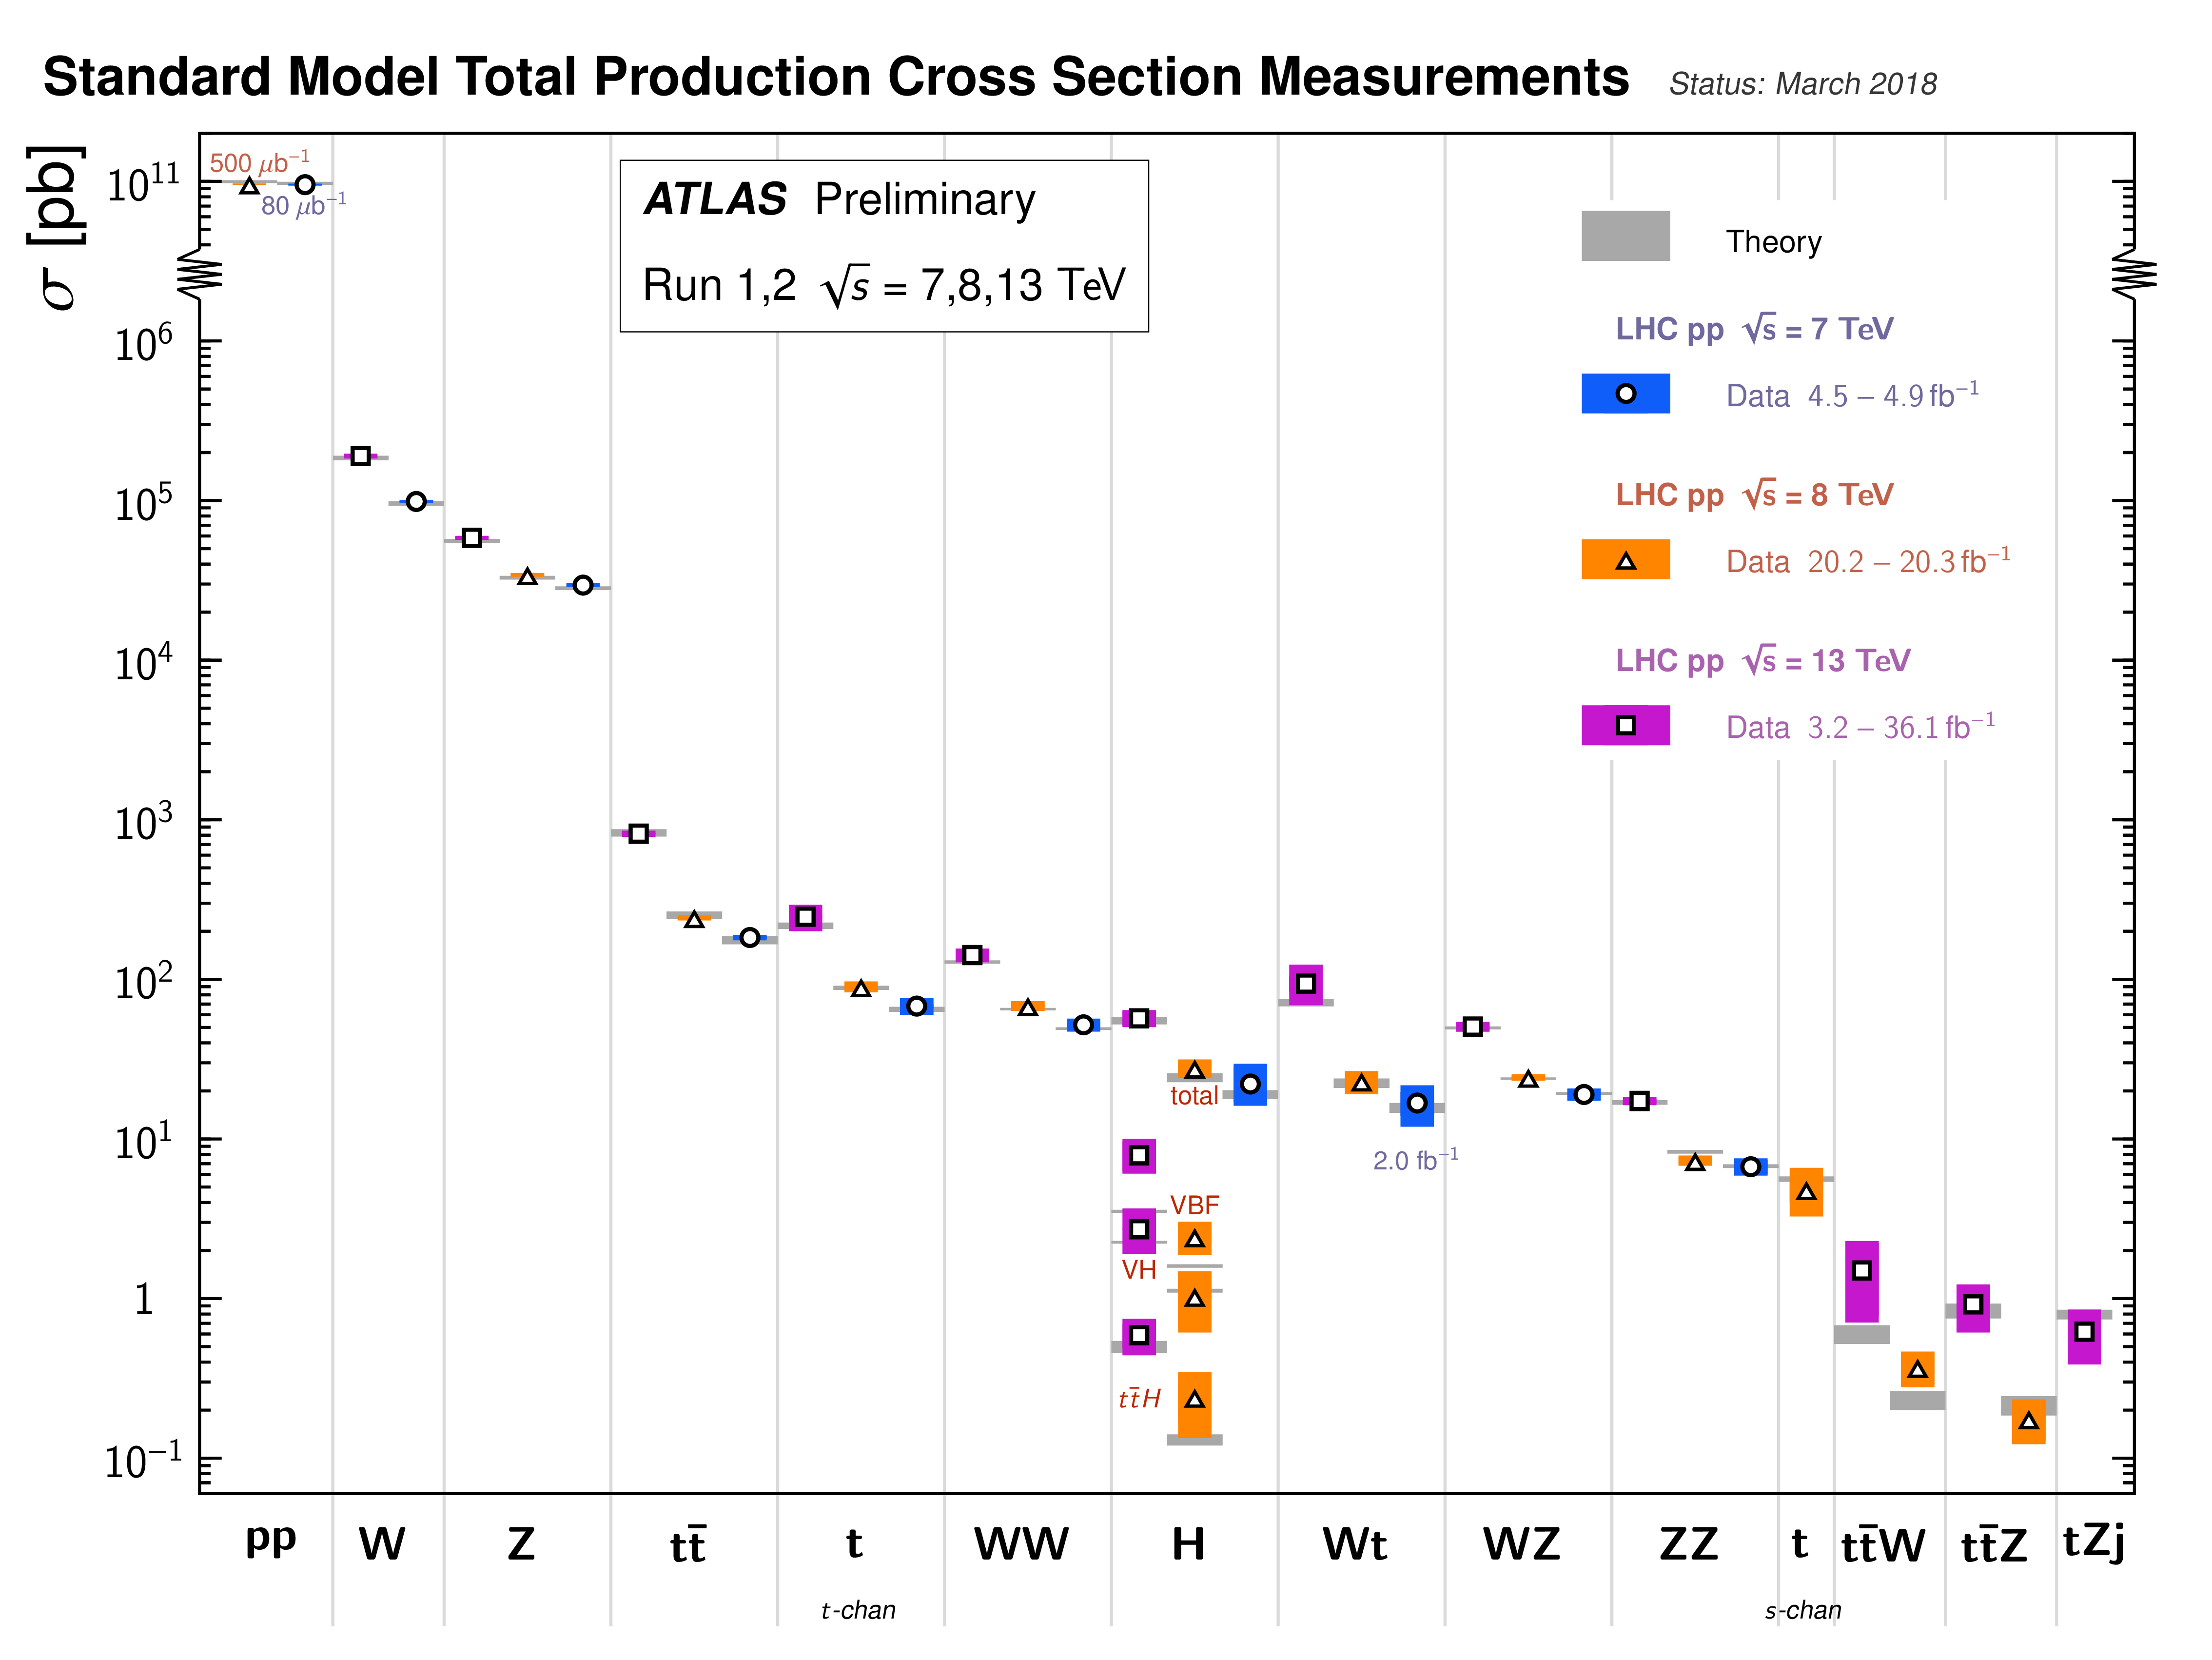
\includegraphics[width=0.6\linewidth]{sm_xsec_summary}
\caption{Summary of Standard Model production cross sections measured by ATLAS, compared to theoretical predictions~\cite{sm-summary-plots}.}
\label{fig:sm_xsec_summary}
\end{figure}

The Standard Model is expressed in the language of Quantum Field Theory.
The theory consists of three generations of matter fields, specified by their representation under the gauge group $SU(3)\times SU(2)\times U(1)$ and the Poincar\'e group, as well as a complex scalar field.
Poincar\'e symmetry consists of the Lorentz symmetry of special relativity, plus global translational symmetry.

The Standard Model is a complete theory in the sense that it is internally self-consistent,
and all particles predicted by the theory have been observed experimentally.
However, the Standard Model does not account for all known physical phenomena,
and so cannot be considered a complete theory of nature.

\section{Electroweak sector and the Higgs mechanism}\label{sec:sm_ew}

The symmetry constraining the electroweak sector of the Standard Model Lagrangian is $SU(2)_L \times U(1)_Y$.
The subscript $L$ for the $SU(2)$ group indicates that it only acts on the left-handed fields in the theory.
Right-handed fields appear as $SU(2)$ singlets.

\subsection{Matter fields}\label{subsec:ew_fields}

All left-handed matter fields are $SU(2)$ doublets, while their corresponding right-handed fields are $SU(2)$ singlets.
There are three generations of left-handed lepton fields:
\begin{equation}\label{eq:left_handed_leptons}
    \psi_L =
    \begin{pmatrix}
        \nu_e \\ l_e
    \end{pmatrix}_L,\;
    %
    \begin{pmatrix}
        \nu_{\mu} \\ l_{\mu}
    \end{pmatrix}_L,\;
    %
     \begin{pmatrix}
        \nu_{\tau} \\ l_{\tau}
    \end{pmatrix}_L
\end{equation}
and three generations of right-handed lepton fields:
\begin{equation}\label{eq:right_handed_leptons}
\psi_R = e_R,\; \mu_R,\; \tau_R
\end{equation}
Similarly, there are three generations each of the left-handed $SU(2)$-doublet quark fields,
each of which comes in three colors:
\begin{equation}\label{eq:left_handed_quarks}
   \psi_L =
    \begin{pmatrix}
        q_u \\ q_d
    \end{pmatrix}_L,\;
    %
    \begin{pmatrix}
        q_{c} \\ q_{s}
    \end{pmatrix}_L,\;
    %
     \begin{pmatrix}
        q_{t} \\ q_{b}
    \end{pmatrix}_L
\end{equation}
Quark color plays a role in QCD interactions, which will be described in the next section.
There are also the corresponding $SU(2)$-singlet right-handed fields:

\begin{equation}\label{eq:right_handed_quarks}
\psi_R = q_{uR},\; q_{dR},\; q_{cR},\; q_{sR},\; q_{tR},\; q_{bR}
\end{equation}

\subsection{Symmetries and Lagrangian}\label{subsec:ew_lagrangian}

The Lagrangian density satisfying the required symmetries, including all renormalizable terms, can be written as:
\begin{equation}\label{eq:ew_lagrangian}
    \mathcal{L}_{EW} = \mathcal{L}_{kin} + \mathcal{L}_{\text{interactions}}
\end{equation}
where the kinetic part of the electroweak Lagrangian is:
\begin{equation}\label{eq:ew_kin}
    \mathcal{L}_{kin} = -\frac{1}{4}W^{\mu \nu}_{a}W_{\mu \nu}^{a}-\frac{1}{4}B^{\mu \nu}B_{\mu \nu}
\end{equation}
$W_\mu^a$ are the three $SU(2)_L$ gauge bosons, $B_\mu$ is the $U(1)_Y$ (hypercharge) gauge boson, and $W_{\mu\nu} = \partial_{\mu} W_{\nu} - \partial_{\nu} W_{\mu}$.
The part of the electroweak Lagrangian describing electroweak interactions is:
\begin{equation}\label{eq:ew_int}
    \mathcal{L}_{\text{interactions}} = \sum_{\text{generations}}\left[\frac{g}{2}\bar{\psi}_{L}\gamma^\mu\sigma^i W_\mu^i \psi_L+
    g'B_\mu\left(Y_{\psi_L}\bar{\psi}_L\gamma^\mu\psi_L + Y_{\psi_R}\bar{\psi}_R\gamma^\mu \psi_R\right)\right]
\end{equation}
where $\gamma^\mu$ are the Dirac gamma matrices, and Y is the hypercharge associated with the relevant field.

Left-handed leptons and quarks have weak hypercharge $Y = -1$ and $Y = 1/3$, respectively.
Right-handed leptons have weak hypercharge $Y = -2$. Right-handed up-type quarks have weak hypercharge $Y = 4/3$,
and right-handed down-type quarks have weak hypercharge $Y = -2/3$.

This Lagrangian describes the charged-current and neutral-current weak interactions, as well as weak gauge boson self-interactions.
However, it is insufficient to describe nature because the gauge bosons are massless in this theory.
It would be impossible to include gauge boson mass terms in the electroweak Lagrangian without explicitly breaking the symmetry.
Similarly, it's impossible to introduce Lorentz-invariant fermion mass terms that keep the Lagrangian invariant under $SU(2)_L \times U(1)_Y$.
In order to reconcile this theory with the experimentally observed fact of massive weak gauge bosons and massive fermions, a scalar field will have to be introduced to the theory.

\subsection{Spontaneous symmetry breaking}\label{subsec:ew_higgs}

The original $SU(2)_{L}\times U(1)_Y$ symmetry will be spontaneously broken, via the nonzero Higgs vacuum expectation value, to $U(1)_{QED}$.
This process of spontaneous symmetry breaking (SSB) generates fermion masses, electroweak gauge boson masses,
and the Yukawa coupling terms between fermions.
It also generates a new massive real scalar field, known as the Higgs field.
We can introduce a new $SU(2)$-doublet complex scalar field, $\phi$, as well as a potential of the form:
\begin{equation}\label{eq:higgs_potential}
    V(\phi) = \mu^2 \phi^\dagger\phi + \lambda(\phi^\dagger\phi)^2
\end{equation}
with $\lambda > 0$ and $\mu^2 <0$.
The minimum energy state satisfies: $\phi^\dagger\phi = \frac{-\mu^2}{2\lambda}$.
We can then re-parameterize the scalar field as:
\begin{equation}\label{eq:higgs_param}
    \phi = \exp{\left(i\frac{\sigma_i}{2}\theta^i(x)\right)}\frac{1}{\sqrt{2}}\begin{pmatrix} 0 \\ v+H(x) \end{pmatrix}
\end{equation}
where $H(x)$ and $\theta^i(x)$ are real-valued fields, and $v = \sqrt{\frac{-\mu^2}{\lambda}}$ is the vacuum expectation value of the Higgs field.
Because of the $SU(2)_L$ symmetry of the theory, we are free to choose convenient values for $\theta^i(x)$,
without affecting the outcome of any observable predictions.
Selecting $\theta^i(x) = 0$, the additional kinetic term required in the Lagrangian is:
\begin{equation}\label{eq:higgs_kinetic}
    \Delta\mathcal{L}_{EW} = \left(D_{\mu}\phi\right)^{\dagger}\left(D_{\mu}\phi\right)
    =\frac{1}{2}\partial_{\mu}H \partial^{\mu}H + \frac{1}{2}(v+H)^{2}\left(\frac{g^2}{4}W_\mu^\dagger W^\mu
    + \frac{g^2}{4\cos^2 {\theta_W}}Z_\mu Z^\mu\right)
\end{equation}
where $W_\mu$ and $Z_\mu$ are mass eigenstates of the electroweak gauge fields.
Each mass eigenstate is a linear combination of the original $W_\mu^a$ and $B_\mu$.
This results in interaction terms between the Higgs field and the $W$ and $Z$ bosons, as well as quadratic terms for these same bosons.
A quadratic term in the Lagrangian is physically the same as having a mass term in the Lagrangian.
So we find that the $W$ and $Z$ boson masses are:
\begin{equation}\label{eq:wz_masses}
    M_w = \frac{1}{2}vg,\; M_Z = \frac{M_W}{\cos{\theta_W}}
\end{equation}
Thus, through spontaneous symmetry breaking, electroweak gauge boson masses are generated without explicit mass terms in the Lagrangian.
The introduction of this scalar field and its associated potential also generates fermionic mass terms, couplings between the fermions and the scalar field, and a mass term for the scalar field itself.
Like with the gauge bosons, adding an explicit fermionic mass term would have broken the $SU(2)_L \times U(1)_Y$ symmetry of the theory.
However, the introduction of the new scalar field allows for additional terms in the Lagrangian, which can be written, in unitary gauge, as:
\begin{equation}\label{ew:yukawa_lagrangian}
    L_Y = \frac{1}{\sqrt{2}}\left(v+H\right)\left(c_{1}\bar{d}d+c_2\bar{u}u+c_3\bar{e}e\right)
\end{equation}
Once again, after spontaneous symmetry breaking, there appear terms in the Lagrangian that are quadratic in the fields.
These are mass terms for the fermions.
As with the gauge bosons, fermion masses are proportional to the Higgs vacuum expectation value:
\begin{equation}\label{ew:fermion_masses}
    m_d = -c_1\frac{v}{\sqrt{2}},\; m_u = -c_2\frac{v}{\sqrt{2}},\; m_e = -c_3\frac{v}{\sqrt{2}}
\end{equation}
Unlike for the gauge bosons, we find no testable relationship between fermion masses, since the coefficients are independent free parameters of the theory.

The Higgs mechanism allows for the generation of masses for fermions and electroweak gauge bosons without explicitly breaking the original symmetry of the theory.
Additional consequences arising from the Higgs mechanism are the relationship between $Z$ and $W$ boson masses, the existence of a new massive scalar field, and interactions between this field and the fermions and gauge bosons.
The massive particle associated with this field, the Higgs boson, was discovered in 2012 by the ATLAS and CMS collaborations~\cite{sm-higgs-discovery-atlas,sm-higgs-discovery-cms}.

\section{Quantum Chromodynamics}\label{sec:sm_qcd}

Quantum Chromodynamics (QCD) is the part of the Standard Model concerned with strong interactions.
Because protons are bound states of quarks and gluons, QCD is needed for making any calculation of event rates at a proton-proton collider.
It's especially important for understanding the behavior of jets, which will be described in detail in chapter~\ref{ch:jets}.
The particular structure of the theory yields very different behavior at high energy and low energy.
At high energy, where the coupling strength is low, quarks and gluons are only weakly bound, so the theory behaves as an approximately free theory, a property known as asymptotic freedom.
At lower energies, the coupling strength grows, and quarks and gluons become strongly bound, a property known as confinement.

\subsection{Matter fields}\label{subsec:matter fields}

The fields involved are the quark fields, which also participate in electroweak interactions.
In the case of QCD, the quarks are in the fundamental $\boldsymbol{3}$ representation of $SU(3)$:
\begin{equation}\label{eq:qcd-fields}
    \psi = \begin{pmatrix}\psi_R \\ \psi_G \\ \psi_B \end{pmatrix}
\end{equation}
where $R,\;G,\;B$ stand for the red, green, and blue color charges.
The theory will be invariant under local transformations in this color space.

\subsection{Symmetries and Lagrangian}\label{subsec:qcd_lagrangian}
Like the electroweak theory, QCD is a non-Abelian gauge theory.
The Lagrangian is generated by positing the transformations under which the Lagrangian is invariant,
and including all terms that respect these symmetries.
For QCD, the symmetry group is $SU(3)$, yielding the following Lagrangian:
\begin{equation}\label{eq:qcd-lagrangian}
    \mathcal{L}_{QCD} = \sum_{generations}i\bar{\psi}D_\mu\gamma^\mu\psi-\frac{1}{4}G_{\mu\nu}^a G_a^{\mu\nu}
\end{equation}
where
\begin{equation}\label{eq:qcd-derivative}
D_\mu = \partial_\mu - i g_s G_\mu^a T^a
\end{equation}
is the gauge-covariant derivative, $g_s$ is the strong coupling constant, $G_\mu^a$ are the eight gluon fields,
and $T^a$ are the infinitesimal generators of $SU(3)$.
The gluon field strength tensor, $G_{\mu\nu}^a$, is defined as:
\begin{equation}\label{eq:qcd-field-strength}
    G_{\mu\nu}^a = \partial_\mu G_\nu^a - g_s f^{abc} G_\mu^b G_\nu ^c
\end{equation}
where $f^{abc}$ are the $SU(3)$ structure constants.
This Lagrangian describes the kinematics of massless quarks, their interactions with gluons, and gluon self-interactions.
Quarks are given mass through electroweak symmetry breaking, as described in~\ref{subsec:ew_higgs}.

\subsection{QCD coupling constant}\label{subsec:qcd_coupling}
The value of the strong coupling constant, $g_s$, depends on the energy scale of the process under consideration.
The rate of change of the coupling as energy increases is governed by the $\beta$ function,
\begin{equation}\label{eq:sm-qcd-beta}
    \beta\left(\alpha_s\right) = \frac{\alpha_s}{2\pi}\left(\frac{11}{3}n_{\text{colors}}-\frac{4}{3}n_{\text{flavors}}\right)
\end{equation}
where $\alpha_s = g_s^2 / 4\pi$.
In QCD, there are three colors and three flavors, the consequence of which is that the coupling constant decreases with energy.
This is known as the "running" of the coupling constant, and results in very different predictions for the theory at different energy scales.
Figure~\ref{fig:sm_qcd_coupling} shows the predicted value of $\alpha_s$ over a range of energies, along with values measured through a variety of physics processes.

\begin{figure}[!ht]
    \centering
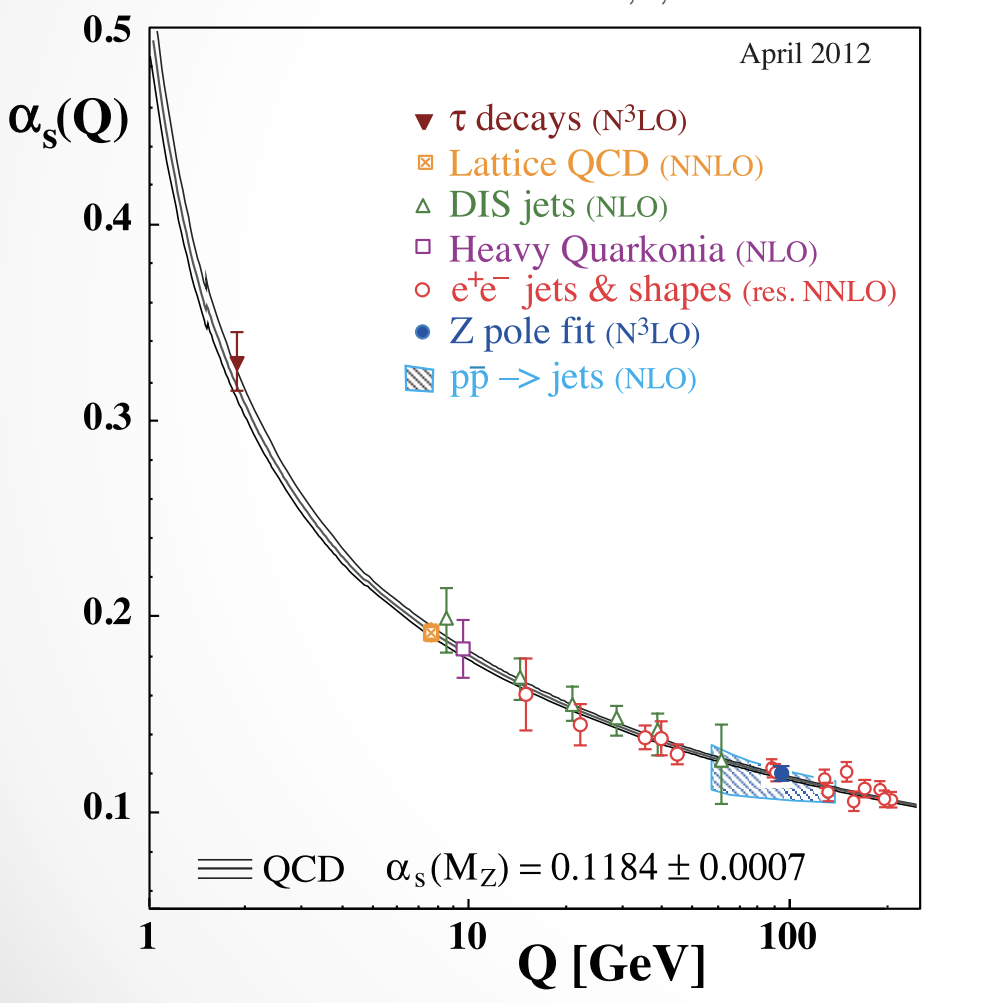
\includegraphics[width=0.6\linewidth]{sm_qcd_coupling}
\caption{Measured values of the strong coupling constant $\alpha_s$ and its predicted values across a range of energies~\cite{sm-review-2014}.}
\label{fig:sm_qcd_coupling}
\end{figure}

\subsubsection{Asymptotic freedom}

At high energies, at or above the $GeV$ scale, the strong coupling constant becomes small.
As a result, QCD calculations in this regime are \textit{perturbative}, meaning they can be approximated by a finite sum of terms expanded in powers of the coupling constant.
This is similar to the way calculations are done in quantum electrodynamics (QED).

Asymptotic freedom means that as energy grows infinite, quarks and gluons can be treated as completely un-coupled, free particles.
At very high energies, their interactions can be treated as small perturbations about the free theory.
At the LHC, the hard-scattering cross-section of a quark from one proton colliding with a quark from another proton can be calculated in this perturbative way.
However, the full proton-proton collision cross-section calculation requires a combination of both perturbative and non-perturbative calculations.

\subsubsection{Confinement and Hadronization}

At lower energies, the strong coupling constant grows larger, and the theory can no longer be treated as perturbative.
Because the coupling constant is large, a finite series expanded in powers of the coupling constant is no longer sufficient to estimate the full predictions.
Instead, higher-order terms grow larger and larger, which means an infinite number of such terms would be needed to make an accurate prediction.
As can be seen in figure~\ref{fig:sm_qcd_coupling}, perturbation theory begins to fail below $\approx1~GeV$.

Confinement is a consequence of the large coupling constant at low energies.
Since quarks and gluons are strongly coupled, they can no longer exist as free states.
Instead, they can only exist as color-neutral bound states, called hadrons.
In a collision event, when a quark is generated in the final state, the strong force between the quark and other quarks in the event remains constant as distance between them increases.
Equivalently, the potential energy between quarks increases with distance.
Eventually it becomes energetically favorable for new quarks to be created from the vacuum, with the correct color charge to neutralize the color charge of the escaping quark.
These new particles become bound together in color-neutral free states.
This process is known as hadronization.
Experimental evidence suggests that hadronization occurs at energies of a few hundred $MeV$.

Hadronization, along with parton showering, is responsible for the emergence of jets from LHC collisions.
Rather than observing the quarks and gluons produced in the collision,
the detector can only observe the spray of hadrons that result.
Jets will be discussed in detail in chapter~\ref{ch:jets}.
Confinement has not been rigorously proven from a theoretical standpoint.
However, the existence of color confinement is consistent with empirical evidence.

\subsection{Parton distribution functions}\label{subsec:qcd_pdfs}

The QCD Lagrangian describes how individual quarks and gluons behave.
But the LHC collides protons, not individual quarks.
Protons consist of three valence quarks: two up quarks and one down quark, and a "sea" of quarks, antiquarks, and gluons.
When calculating collision cross-sections for the LHC, the internal structure of the protons must be taken into account.

This internal structure is accounted for using parton distribution functions (PDFs).
PDFs are expressed as probability density functions $f_i(x, Q^2)$, where $i$ denotes the flavor of the parton, $x$ is the fraction of momentum carried by the parton, and $Q$ is the momentum transfer at which the proton structure is probed, or the energy scale of the hard-scatter process.
The values of these PDFs cannot be calculated from first principles, but thanks to the QCD factorization theorem, they can be measured experimentally.
The factorization theorem allows for the cross section to be factorized into a hard-scattering part and a normalization factor from the PDFs.
By comparing the experimental and theoretical cross sections for a given process, the PDFs can be inferred.
Since the PDFs are independent of the hard-scattering process, the data from a variety of processes can be combined.
Using the  Dokshitzer-Gribov-Lipatov-Altarelli-Parisi (DGLAP) equations~\cite{sm-dglap}, which describe how the PDFs depend $Q^2$, data from different processes at different momentum-transfer scales can all be combined into a global fit.
For PDFs used by ATLAS, the global fit includes data from deep inelastic scattering (DIS) $e-p$ collisions from the HERA-II experiment, jet and $t\bar{t}$ production from ATLAS and CMS, and observables from several other processes~\cite{sm-pdf-atlas-run2}.

Figure~\ref{fig:sm_pdfs} shows the proton PDFs evaluated at NLO for $Q^2 = 10~GeV^2$ and $Q^2 = 10^{4}~GeV^2$
\begin{figure}[!ht]
    \centering
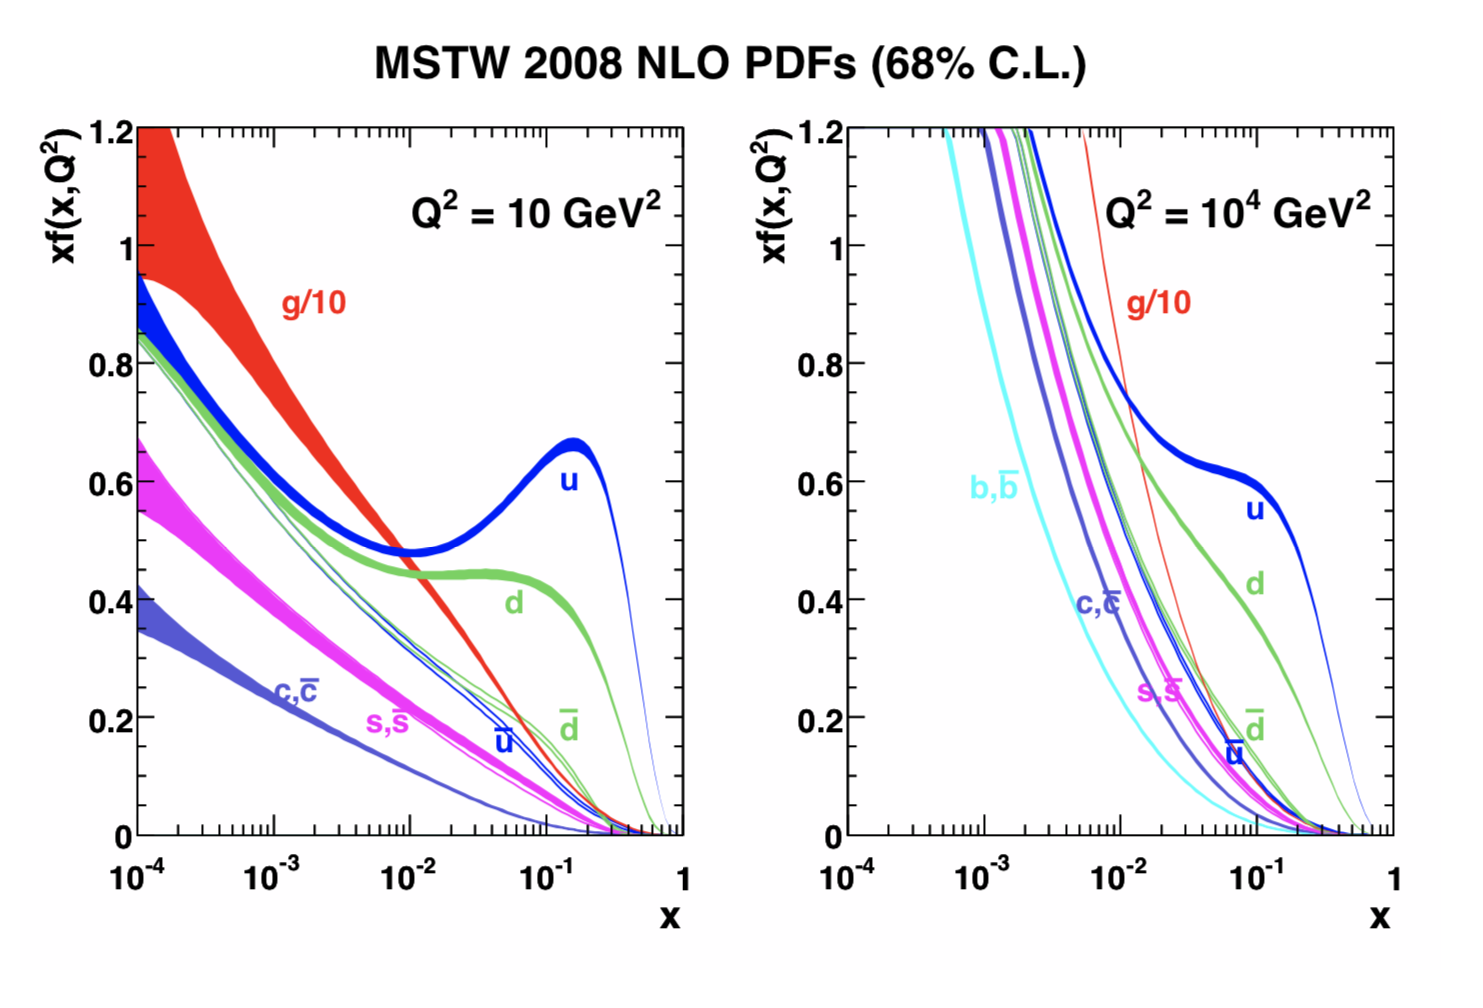
\includegraphics[width=0.6\linewidth]{sm_pdfs}
\caption{Parton distribution functions for the proton, evaluated at NLO for two different energy scales~\cite{sm-pdf-2009}.}
\label{fig:sm_pdfs}
\end{figure}

When calculating LHC cross-sections, the hard-scattering cross-section for different types of partons
must be convolved with the PDFs for each parton.
The proton-proton cross-sections are thus an average of partonic cross-sections, weighted by the PDFs for those partons.

\section{Limitations}\label{sec:sm_limits}

Experimental tests of the Standard Model to date have shown no significant deviations from its predictions,
across a very wide range of physical processes and energy scales~\cite{sm-summary-plots}.
However, it is quite clear that the Standard Model is not a complete theory of nature.
There are many problems and questions that it leaves unanswered.

\subsection{Fine tuning and the Higgs mass}\label{subsec:sm_hierarchy}

The Higgs field, which is responsible for the mass of all fundamental fermions and the massive electroweak gauge bosons, was confirmed by the discovery of $125~GeV$ Higgs boson by ATLAS and CMS in 2012~\cite{sm-higgs-discovery-atlas,sm-higgs-discovery-cms}.
The fact that the Higgs mass should be so small is an unsolved mystery of particle physics.
When performing QFT calculations, there often arise terms in the perturbation expansion that are formally infinite.
A procedure known as renormalization is used in order to tame these divergences.
One method of renormalization involves cutting off the divergent integrals at some scale, $\Lambda$, then canceling the infinities by redefining some of the free parameters of the theories.

When calculating the physical mass-squared of the Higgs, there are some terms in the series which are proportional to the square of the cutoff scale.
The cutoff scale is considered to be some very large energy scale, usually the Planck energy $10^{19}~GeV$.
As a result, an infinite sum of positive and negative terms with absolute values on the order of $10^{38}~GeV^2$ must cancel out to yield physical Higgs mass-squared, which is on the order of $10^4~GeV^2$.
This kind of cancellation is philosophically unsatisfying, because it seems to be an unreasonable amount of fine-tuning~\cite{sm-higgs-naturalness}.

The fine-tuning is closely related to the so-called "hierarchy problem".
Why is gravity so much weaker than the other fundamental forces?
That is, why do we observe $G_F \gg G_N$?
Since $G_F \propto 1/{M_W^2}$, and $G_N \propto 1/\Lambda_{Pl}^2$ and because $M_W$ is proportional to the Higgs vev, the Higgs-mass fine-tuning and the hierarchy problem are really the same thing.
A possible way to avoid fine tuning and the hierarchy problem comes from Supersymmetry, which will be covered in chapter~\ref{ch:susy}

\subsection{Grand unification}\label{subsec:sm_unification}

The symmetry groups and representations of the Standard Model have great explanatory power, but they are, at heart, axiomatic rather than derived.
And the Standard Model contains a large number of free parameters, the values of which are not explained by the model, but must be measured by experiment.
It's possible that a simpler model could be found, one which embeds the baroque structure of the Standard Model in a much simpler set of symmetry groups and representations.
Such an idea is known as \textit{Grand Unification}.
A Grand Unified Theory (GUT) would predict relationships between some of the free parameters of the Standard Model, resulting in a simpler and more elegant theory.
This would be analogous to electroweak unification, which explains the relationship between $W$ and $Z$ boson masses and their couplings, and results in a theory with only three free parameters.

A GUT would explain all particle interactions with a single symmetry group.
This symmetry would be broken below some energy scale to the $SU(3)_C \times SU(2)_L \times U(1)_Y$ symmetry of the Standard Model.
The details of the symmetry breaking process would yield relations between the strong and electroweak coupling constants~\cite{sm-gut}.
Going a step further, if gravitational interactions could also be incorporated into this single theory, it would be a so-called "Theory of Everything" (TOE).
A very popular TOE candidate, known as String Theory, requires the existence of Supersymmetry.

\subsection{Dark matter}\label{subsec:sm_dark_matter}

The type of matter explained by the Standard Model is known to account for approximately $20\%$ of the matter in the universe.
The remaining $80\%$ exists in the form of dark matter.
The exact explanation for dark matter is not yet known, those many of its properties can be inferred.
It is massive and invisible, and its primary interaction with visible matter is through gravity~\cite{sm-pdg-dark-matter}.
Dark matter is known to be massive, because it interacts gravitationally.
This can be seen in its effect on the rotation curves of galaxies, gravitational lensing of distant galaxies,
and on the anisotropy of the Cosmic Microwave Background Radiation~\cite{sm-kolb-cmb}.

Dark matter could possibly be explained by the Standard Model, if it exists in the form of Massive Compact Halo Objects (MACHOs).
MACHOs are primordial black holes, formed during the very early universe.
If these primordial black holes exist in large enough quantities to account for the majority of dark matter in the universe, they could in principle be detected in gravitational lensing surveys.
However, these surveys have so far failed to observe MACHOs in large enough quantities to account for the known quantity of dark matter.
In fact, dark matter in the form of MACHOs with masses greater than $10^{-7}$ solar masses has been ruled out entirely~\cite{sm-macho-dark-matter}.

Another likely explanation for dark matter is that it is composed of a new fundamental particle, one which is not explained by the Standard Model.
Many versions of Supersymmetry, described in~\ref{ch:susy}, provide a viable dark matter candidate.


\chapter{Supersymmetry} \label{ch:susy}

Supersymmetry (SUSY) is an extension to the Standard Model, which introduces a new spacetime symmetry relating fermionic and bosonic fields~\cite{sm-pdg-dark-matter}.
It is a remarkable theory, which has the potential to resolve many of the known problems of the Standard Model in one fell swoop.

\section{Motivation for New Physics}\label{sec:susy_motivation}

As described in~\ref{sec:sm_limits}, the Standard Model leaves open some very important questions.
These mysteries all point towards a more fundamental theory, one which is applicable at short distances scales, or equivalently, higher energies.
The most important task of this new theory is to explain why the Higgs mass is so small, without resorting to the extreme amount of fine-tuning required by the Standard Model.
But a more fundamental theory of particle physics could potentially simplify the symmetry structure of the model and provide an explanation for the seemingly arbitrary quantum numbers of the Standard Model particles.
This new theory should not be seen as a replacement for the Standard Model, but rather an extension of it.
Whatever the new theory is, it should be applicable at very short distance scales, and at low energies, it must reproduce the experimentally-confirmed predictions of the Standard Model.
We know this because all experimental evidence gathered so far indicates the Standard Model is a correct theory up to the energy scales at which it has been probed.
In this view, the Standard Model is considered an effective field theory (EFT), valid below the scale of new physics, $\Lambda_{NP}$.

\subsection{Naturalness}\label{subsec:susy_naturalness}

As explained in~\ref{subsec:sm_hierarchy}, the Standard Model suffers from a problem of extreme fine tuning.
Quadratic diverges in the quantum corrections to the Higgs mass-squared require the bare mass of the Higgs to be
specified to one part in $10^{19}$, which is phenomenally unlikely to happen by chance~\cite{susy-higgs-fine-tuning}.
The quadratic divergences occur in loop diagrams, the largest contribution coming from the top quark loop, shown in figure~\ref{fig:susy_top_loop}.
\begin{figure}[!ht]
    \centering
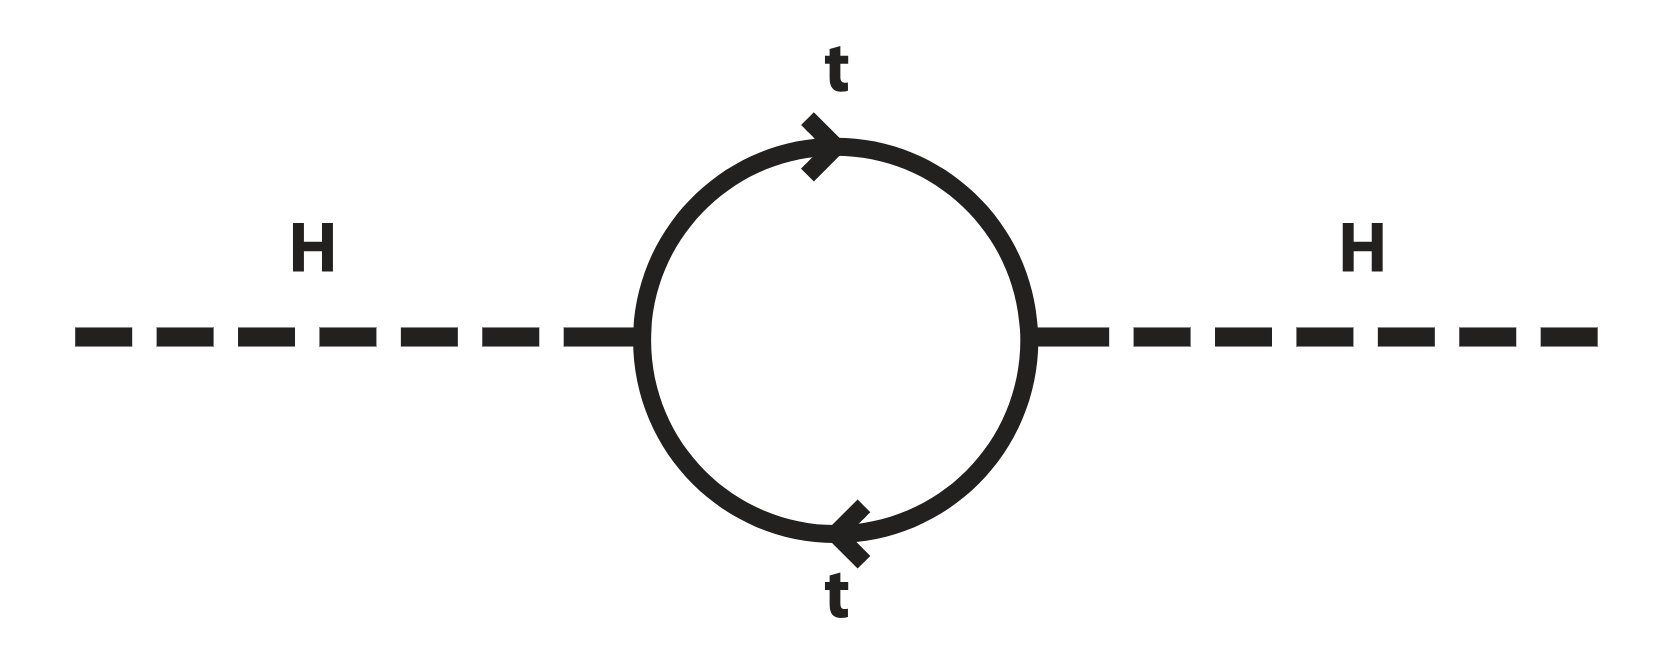
\includegraphics[width=0.6\linewidth]{susy_higgs_top_loop}
\caption{Top-quark loop diagram, the leading correction to the Higgs mass-squared. This contribution is quadratically divergent in the cutoff scale~\cite{susy-primer-1998}.}
\label{fig:susy_top_loop}
\end{figure}
The correction to the Higgs mass-squared coming from this diagram is~\cite{susy-primer-1998}:
\begin{equation}\label{eq:higgs_top_correction}
    \delta m_h^2 = \frac{3m_t^2}{2\pi^2 v^2}\Lambda_{UV}^2
\end{equation}
where $m_t$ is the top quark mass, $v$ is the Higgs vacuum expectation value, and $\Lambda_{UV}$ is the ultraviolet cutoff.

Supersymmetry introduces a so-called superpartner for each Standard Model particle.
Standard Model fermions have bosonic superpartners, and Standard Model bosons have fermionic superpartners.
Superpartners always have the same quantum numbers as their Standard Model partners, except for spin.
The details of how this comes about will be discussed in~\ref{sec:susy_theory}.
The superpartner of the top is called the stop.
It's a scalar particle with all the same quantum numbers as the top quark, except for spin.
The introduction of superpartners leads to new quantum corrections to the Higgs mass-squared.
One of those corrections can be seen in~\ref{fig:susy_stop_loop}.
\begin{figure}[!ht]
    \centering
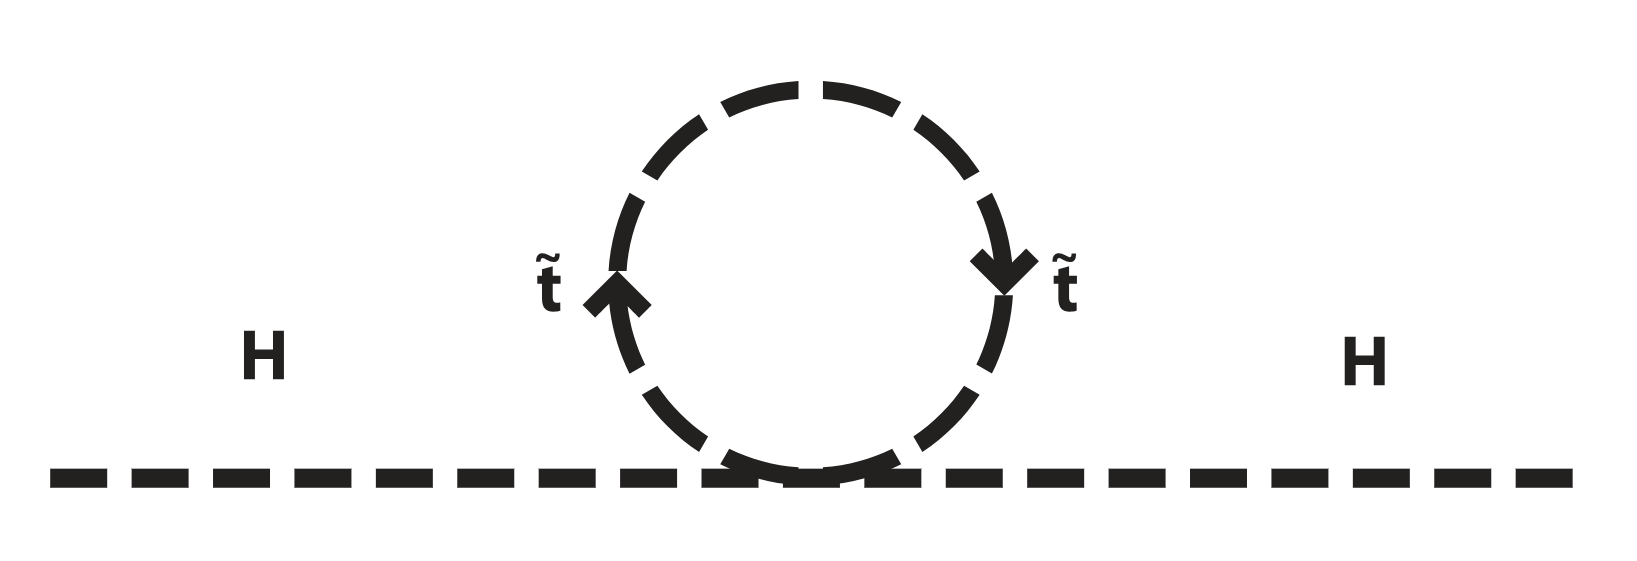
\includegraphics[width=0.6\linewidth]{susy_higgs_stop_loop}
\caption{Stop loop diagram, the leading SUSY correction to the Higgs mass-squared. This contribution is quadratically divergent in the cutoff scale~\cite{susy-primer-1998}.}
\label{fig:susy_stop_loop}
\end{figure}
The correction to the Higgs mass-squared coming from this diagram is~\cite{susy-primer-1998}:
\begin{equation}\label{eq:higgs_stop_correction}
    \delta m_h^2 = -\frac{3m_t^2}{2\pi^2 v^2}\Lambda_{UV}^2
\end{equation}
Thus, the quadratically-divergent top-loop correction is cancelled exactly.
A similar cancellation occurs for all other quadratic divergences in the calculation, leaving terms that are only logarithmically divergent in the cutoff.
In SUSY, the leading correction to the Higgs mass-squared is proportional to the log of the cutoff scale,
and the squared difference between the top and stop masses~\cite{susy-pheno-2000}:
\begin{equation}\label{eq:susy_higgs_correction}
    \delta m_h^2 \propto \left(m_{\tilde{t}}^2 - m_t^2\right)  \Lambda_{UV}
\end{equation}
The amount of fine-tuning required can be quantified by $m_h / \delta m_h $, so in order to preserve naturalness, the stop mass cannot be much heavier than the top quark mass.
If we allow for fine-tuning of only 1 part in 10, then the stop mass shouldn't be higher than the $1~TeV$ scale, which indicates that SUSY should be accessible by the LHC .
Lower bounds on the masses of various suppersymmetric particles from ATLAS range from a few hundred $GeV$ to $2.4~TeV$~\cite{susy-summary-public}.
Figure~\ref{fig:susy_limits_summary} shows a sample of the SUSY particles and decay channels that have been searched for with ATLAS, and the resulting lower bounds.
\begin{figure}[!ht]
    \centering
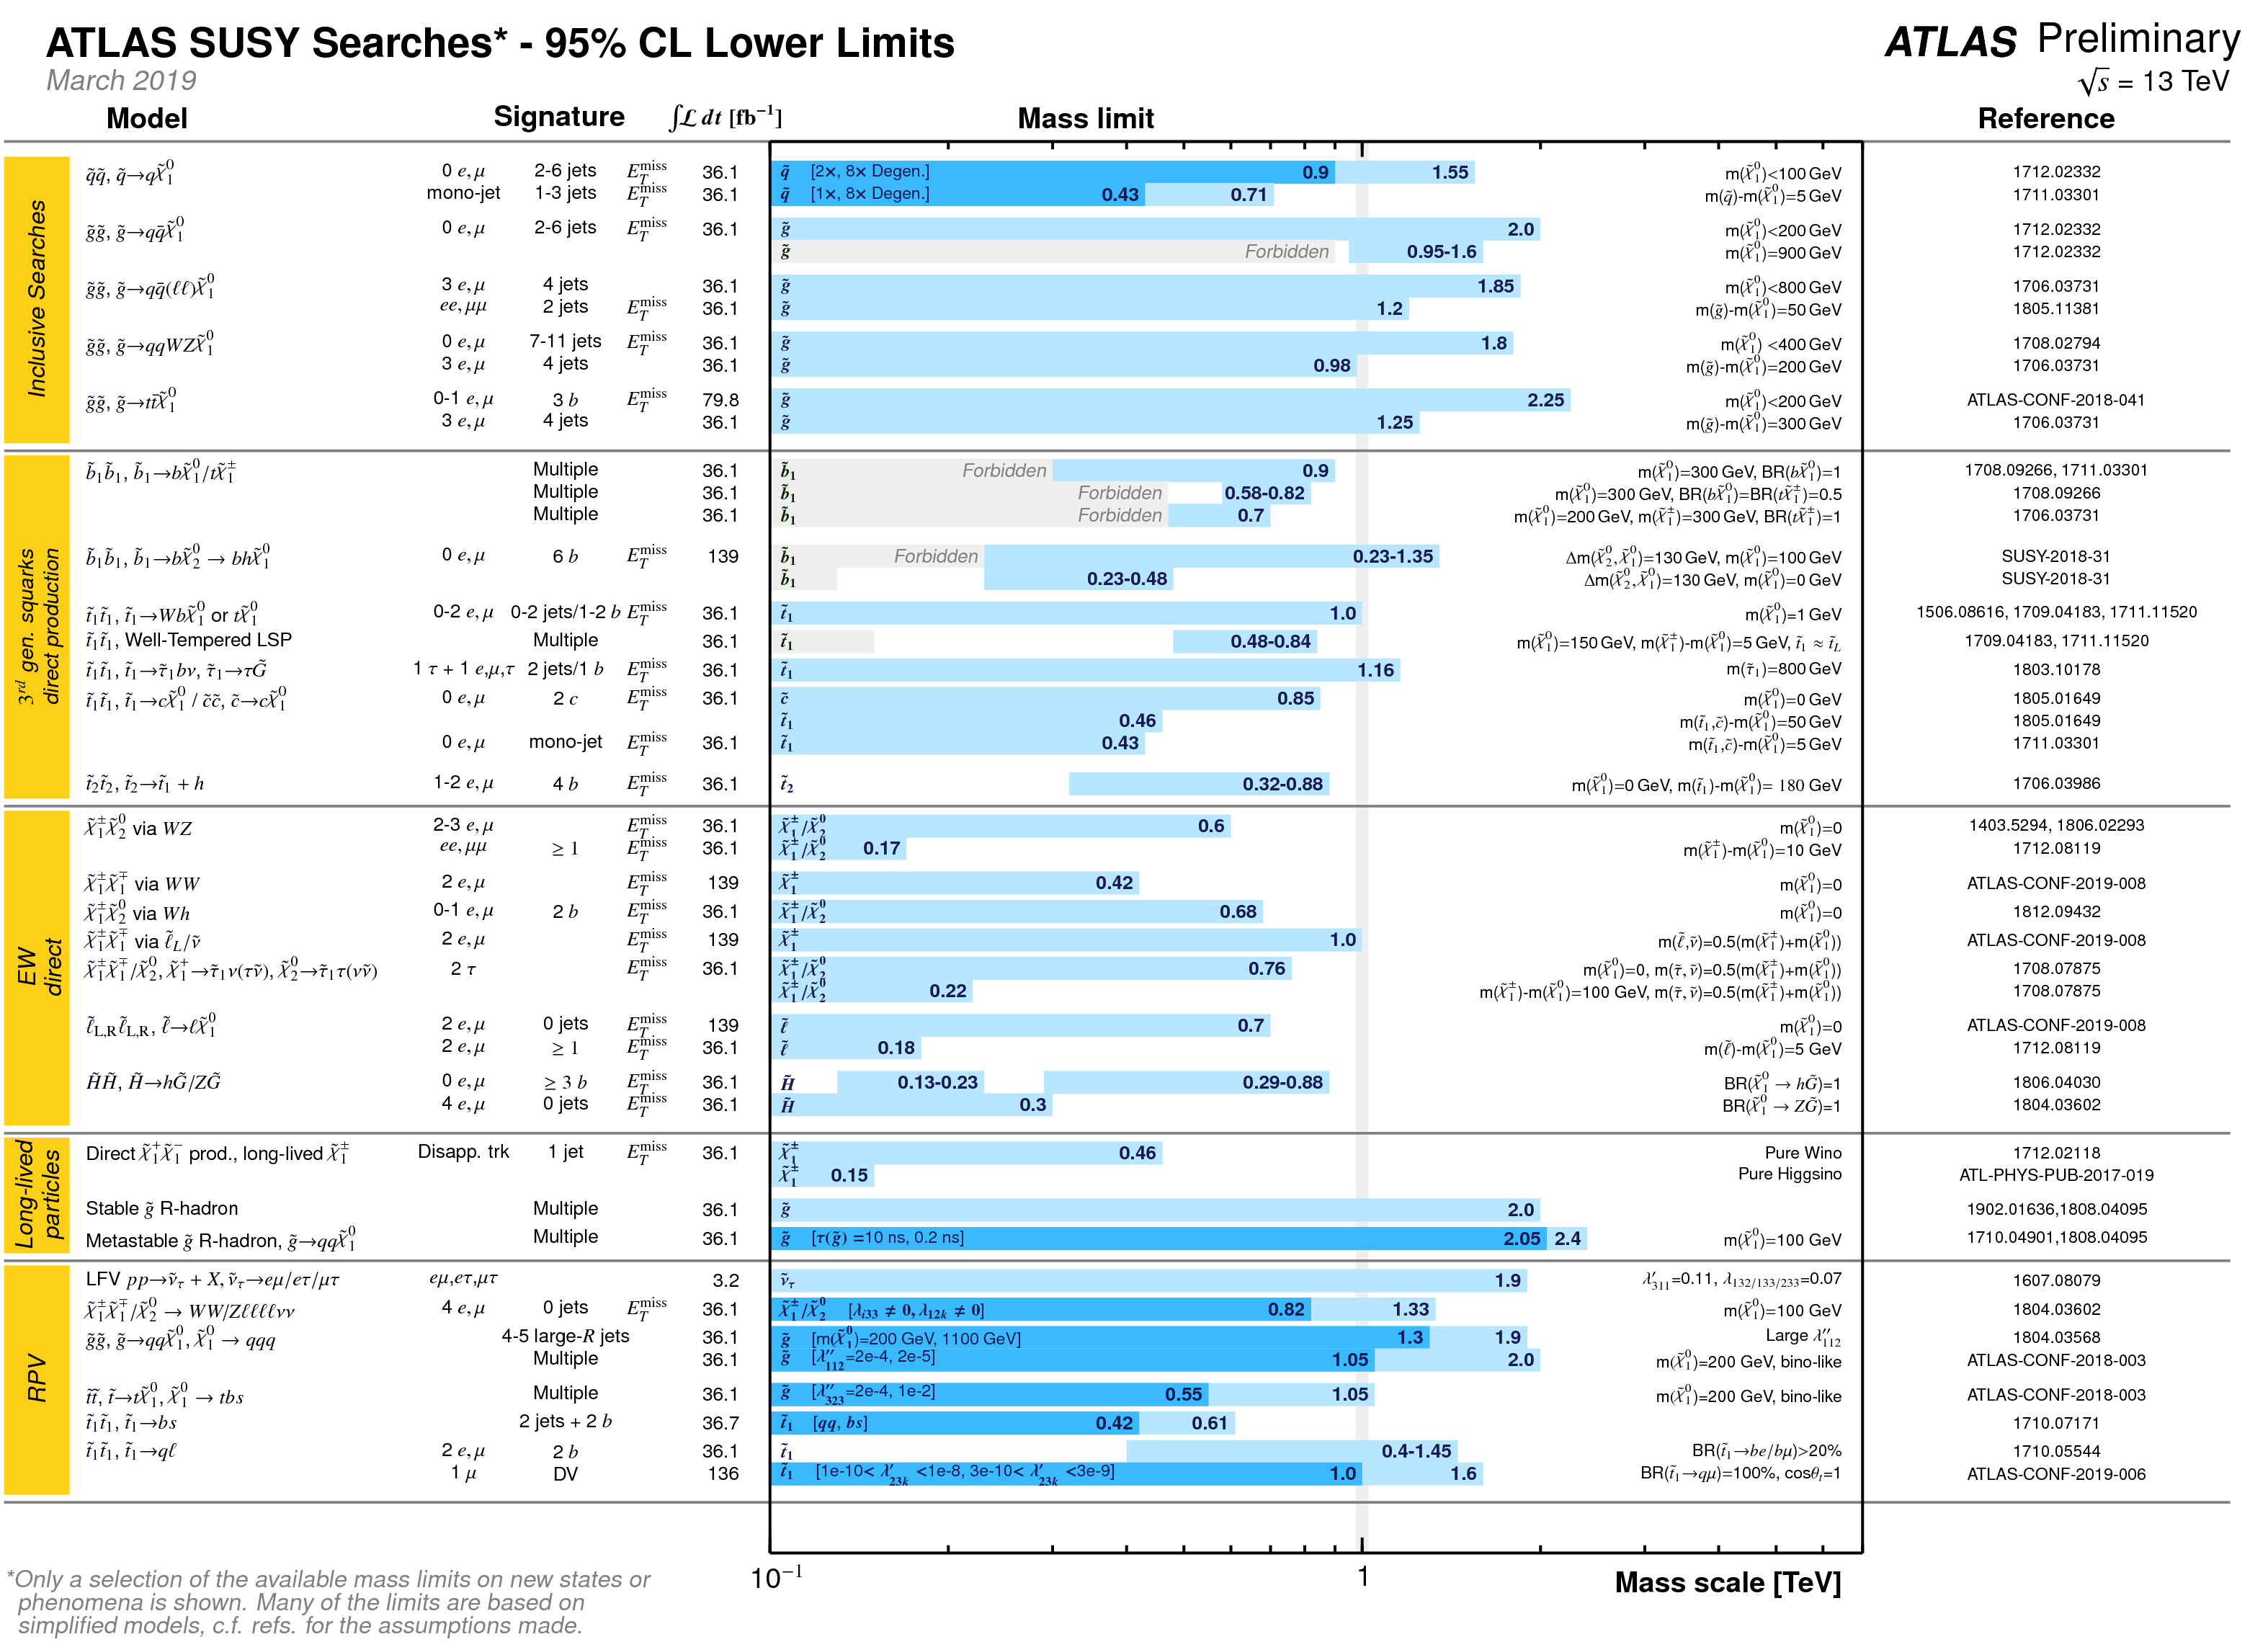
\includegraphics[width=\linewidth]{susy_summary_limits.png}
\caption{A representative sample of the various SUSY searches performed by ATLAS, and their resulting mass lower bounds~\cite{susy-summary-public}.}
\label{fig:susy_limits_summary}
\end{figure}

\subsection{Grand Unification}\label{subsec:susy_unification}

Grand Unification is the idea that the $SU(3)_C \times SU(2)_L \times U(1)_Y$ symmetry of the Standard Model can be embedded in a simpler symmetry group, which constrains the theory at energies above $\Lambda_{GUT}$.
In a Grand Unified Theory (GUT), there would be no distinction between quarks and leptons at energies above $\Lambda_{GUT}$, and the differences in interactions between these two types of matter fields would be explained by the details of the theory and the mechanism by which its symmetry is broken.
Furthermore, at energies above $\Lambda_{GUT}$, the three forces of the Standard Model would be replaced by a single, unified force.
Grand unification would be the logical next step after electroweak unification, in which the electromagnetic and weak forces are shown to be the same force at energies above $\Lambda_{EW}\approx 246~GeV$.
Similarly to how electroweak unification gives a relationship between electric charge and weak isospin, grand unification would give a relationship between color charge and the electroweak quantum numbers.
Several different symmetry groups have been proposed as GUTs.
Among these are $SU(5)$, $SO(10)$, $E_6$, and $SU(5)\times SU(5)$~\cite{susy-unification-1998}.

In order for unification to occur, the value of the three Standard Model coupling constants must converge at some energy scale.
The running of coupling constants is determined by the renormalization group equation (RGE):
\begin{equation}\label{eq:renorm_group}
    \frac{\partial g}{\partial \log \mu} = \beta(g)
\end{equation}
where $g$ is the coupling constant of interest, $\mu$ is the energy scale at which the coupling is being measured, and $\beta$ is a function that depends on the gauge structure and matter content of the theory.
Using the RGE, and measured values of the coupling constants at specific starting energies,
one can calculate the value of the three constants over a large range of energy scales.
For the Standard Model, there is no energy scale at which all three Standard Model constants converge, as would be required for a grand unified theory.
However, when the $\beta$ function is modified to include supersymmetric particles, it is possible for all three Standard Model forces to unify.
In one particular SUSY model, known as the Minimal Supersymmetric Standard Model (MSSM), unification of the forces occurs at $\mu \approx 2\times10^{16}~GeV$~\cite{susy-unification-1998}.
The running of the coupling constants under the Standard Model and MSSM can be seen in figure~\ref{fig:susy_unification}.

\begin{figure}[!ht]
    \centering
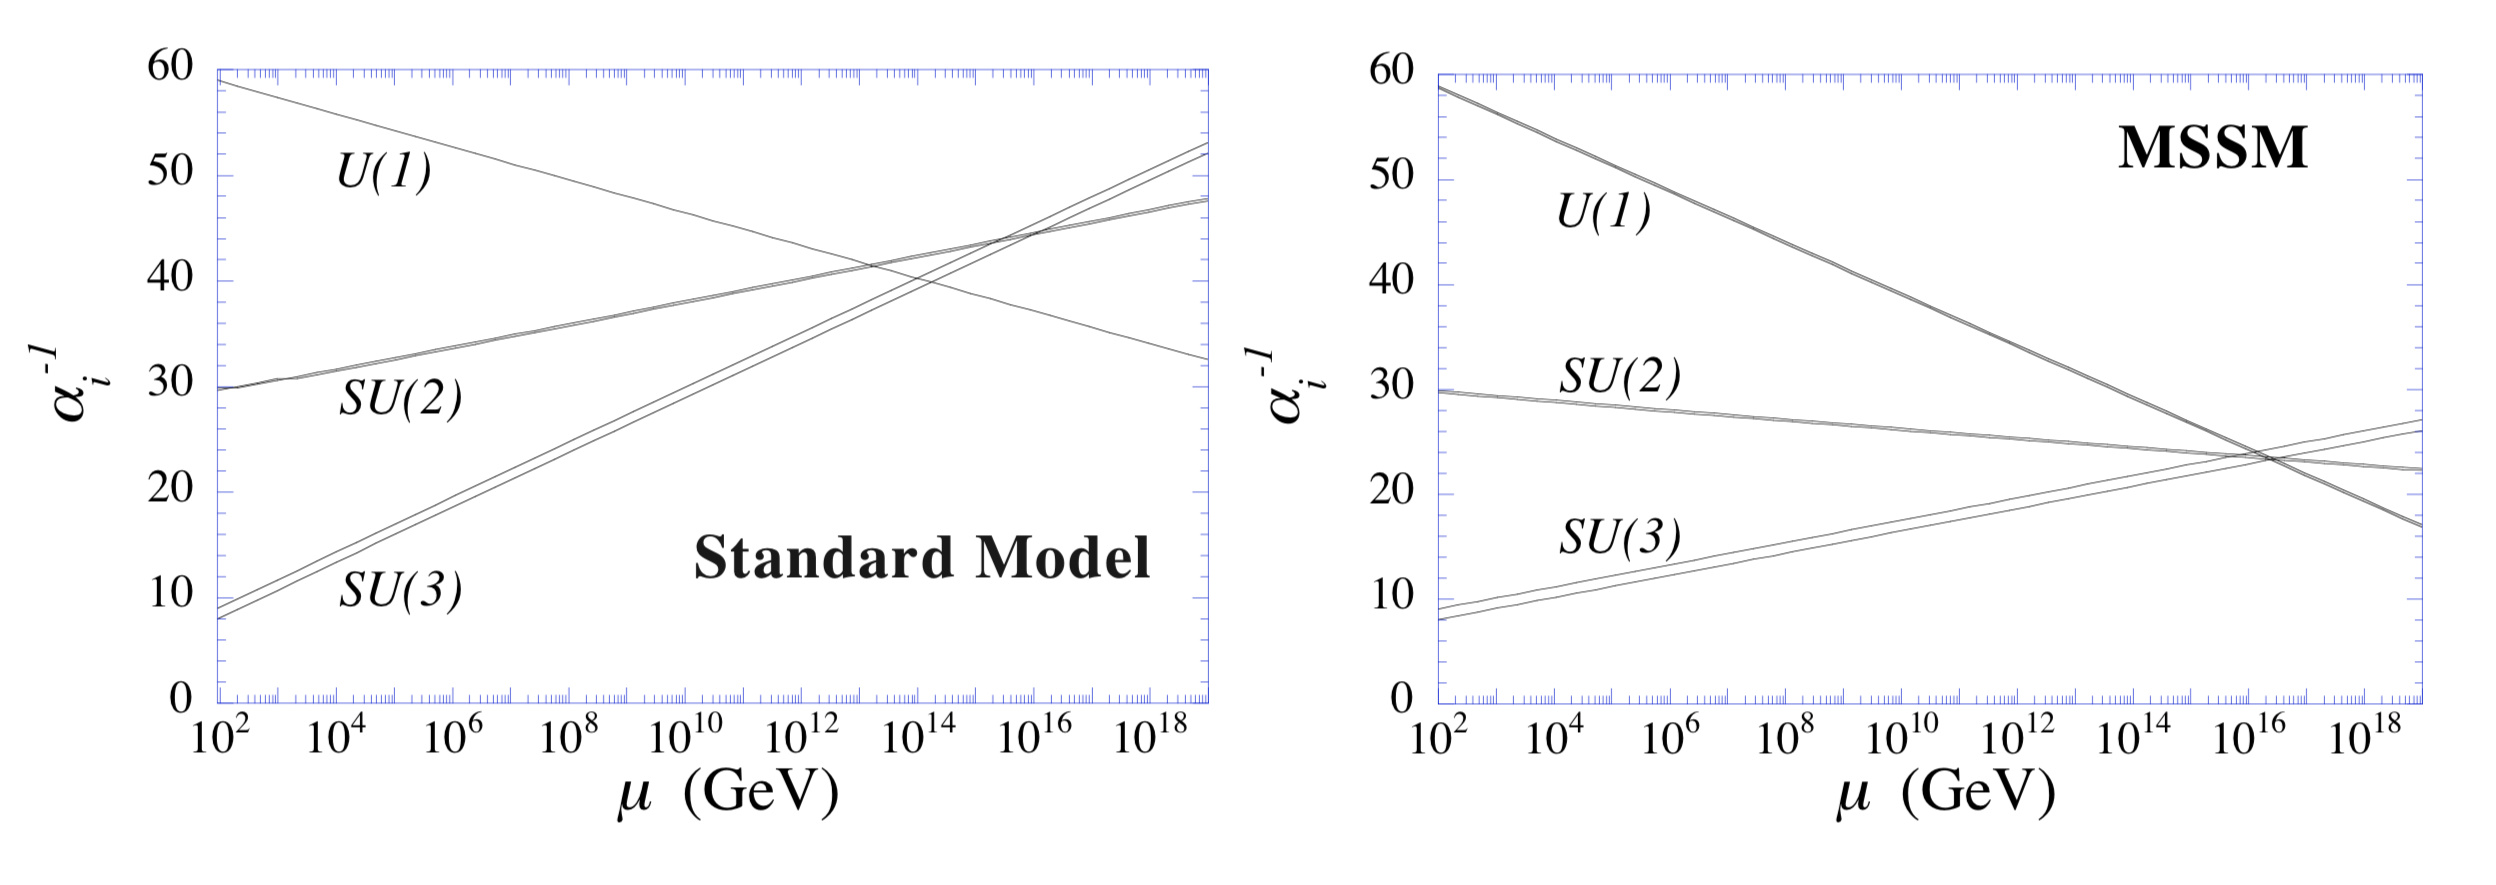
\includegraphics[width=0.95\linewidth]{susy_unification}
\caption{Running of the three Standard Model coupling constants under the Standard Model (left) and MSSM (right) RGEs.
For the MSSM, unification occurs at $\mu\approx 2\times 10^{16}~GeV$~\cite{susy-pheno-2000}.}
\label{fig:susy_unification}
\end{figure}

\subsection{Dark Matter}\label{subsec:susy_dark_matter}

As mentioned in~\ref{subsec:sm_dark_matter}, SUSY can provide an explanation for Dark Matter, which comprises approximately $80\%$ of matter in the universe, but cannot be explained by any known particle.
In SUSY models that conserve R-parity\footnote{See section~\ref{sec:susy_rpv} for a discuss of R-parity and R-parity violation}, the lightest supersymmetric particle (LSP) must be stable because R-parity prevents the LSP from decaying to a final state without SUSY particles, and conservation of energy prevents it from decaying to a final state with SUSY particles.
In so-called "natural" SUSY, the LSP is a neutralino, $\chi_0^{1}$.
The neutralino is a mixture of the electroweak gauge superpartners, the wino and bino, and the Higgs superpartner, the higgsino.
The neutralino in this theory would be stable, massive, electrically neutral, and it would interact via the weak force.
As such, it is a viable candidate for WIMP dark matter.

Intriguingly, if one assumes that dark matter was thermally produced in the early universe, and calculates the required production cross-section to match the dark matter abundance measured today, the result is $\left<\sigma v\right> \approx 3 \times 10^{-26}~cm^{3}/s$, which is very close to what would be expected for a weakly-interacting LSP~\cite{susy-dark-matter-1996}.

\section{Theory and Phenomenology}\label{sec:susy_theory}

Supersymmetry starts by positing a transformation that converts a boson field to a fermion field and vice versa, and a Lagrangian which is invariant under such transformations.
Fields are represented in supermultiplets, each of which always contains a Standard Model particle and its superpartner.
Standard Model bosons are always paired with fermionic superpartners, and Standard Model fermions are always paired with bosonic superpartners.
SUSY transformations commute with all symmetries of the Standard Model, except for the Lorentz transformations.
As a result, a Standard Model particle has all the same quantum numbers as its superpartner, except for spin.
Additionally, SUSY requires both members of the supermultiplet to have the same mass.
Experiments have ruled out the existence of same-mass superpartners for all Standard Model particles, so for SUSY to be compatible with experimental evidence, it must be broken.
The method by which SUSY is broken should have an impact on the phenomenology of the model, specifically on the differences in mass between the Standard Model particles and their superpartners.
A framework called soft SUSY breaking allows for the specifics of the SUSY breaking to be factored out, by adding effective terms to the SUSY Lagrangian which account for the consequences of SUSY breaking without specifying the mechanism.
These new terms break SUSY explicitly, and so this is an effective field theory, valid only at energies well below the SUSY-breaking scale~\cite{susy-soft-1981}.

\subsection{Superfields and superpotentials}\label{subsec:susy_superfields}
Superfields can be categorized into \textit{chiral} and \textit{gauge} superfields.
Standard model fermions and their superpartners will belong to chiral supermultiplets, while Standard Model gauge bosons and their superpartners will belong to gauge supermultiplets.
A generic chiral superfield can be represented as $\Phi(x, \theta)$, where $x$ represents spacetime, and $\theta$ denotes the additional two fermionic degrees of freedom needed for supersymmetry transformations.
It can alternatively be represented as $\Phi = \left(\phi, \psi \right)$, where $\phi$ is the complex scalar component, and $\psi$ is the fermion component.
A generic \textit{vector} superfield can be represented at $V(x, \theta, \bar{\theta})$, where $\bar{\theta}$ are the conjugate degrees of freedom to $\theta$.
In component form, vector supermultiplets can be represented as $V = \left(A^{\mu}, \lambda\right)$, where $A^{\mu}$ is the gauge boson and $\lambda$ is the fermionic superpartner.

The generic supersymmetric action can then be written as~\cite{susy-unification-1998}:
\begin{equation}\label{eq:susy_action}
    S = \int d^4 x \int d^2 \theta d^2 \bar{\theta} \Phi^{\dagger} e^V \Phi
        + \int d^4 x \int d^2 \theta \left(W(\Phi) + W_{\lambda}(V)W_{\lambda}(V)\right)+h.c.
\end{equation}
where the first integrand is the kinetic term for the matter fields, and the second integrand contains the generic superpotential, $W(\Phi)$ and the gauge kinetic term $W_{\lambda}(V)W_{\lambda}(V)$.
The function $W_{\lambda}(V)$ is defined as:
\begin{equation}\label{eq:susy_gauge_potential}
    W_{\lambda}(V) = \mathcal(D)^{2}\bar{\mathcal{D}}V
\end{equation}
where $\mathcal{D} \equiv \partial_{\theta}-i\sigma\dot \partial_x$~\cite{susy-unification-1998}.

\subsection{SUSY particles}\label{subsec:susy_mssm}
In the MSSM, the minimum number of new particles and free parameters are added to the already large assortment of Standard Model ones.
Each Standard Model fermion is paired with a spin-$0$ superpartner, and each Standard Model gauge boson is paired with a spin-$1/2$ superpartner.
For the Higgs boson, introducing a single superpartner is not enough.
There must be at least two Higgs chiral supermultiplets, with hypercharge values $1/2$ and $-1/2$.
This is needed in order to keep the electroweak theory anomaly-free, and for the Higgs mechanism to still give mass to all the fermions~\cite{susy-primer-1998}.

Superpartner states will be denoted with a tilde, and are also referred to as sparticles.
For example, the superpartner of the electron, called the selectron, will be denoted as $\tilde{e}$.
The MSSM chiral superfield content is summarized in table~\ref{tbl:susy_chiral_fields},
and gauge superfields are summarized in table~\ref{tbl:susy_gauge_fields}.
\begin{table}[!ht]
    \centering
  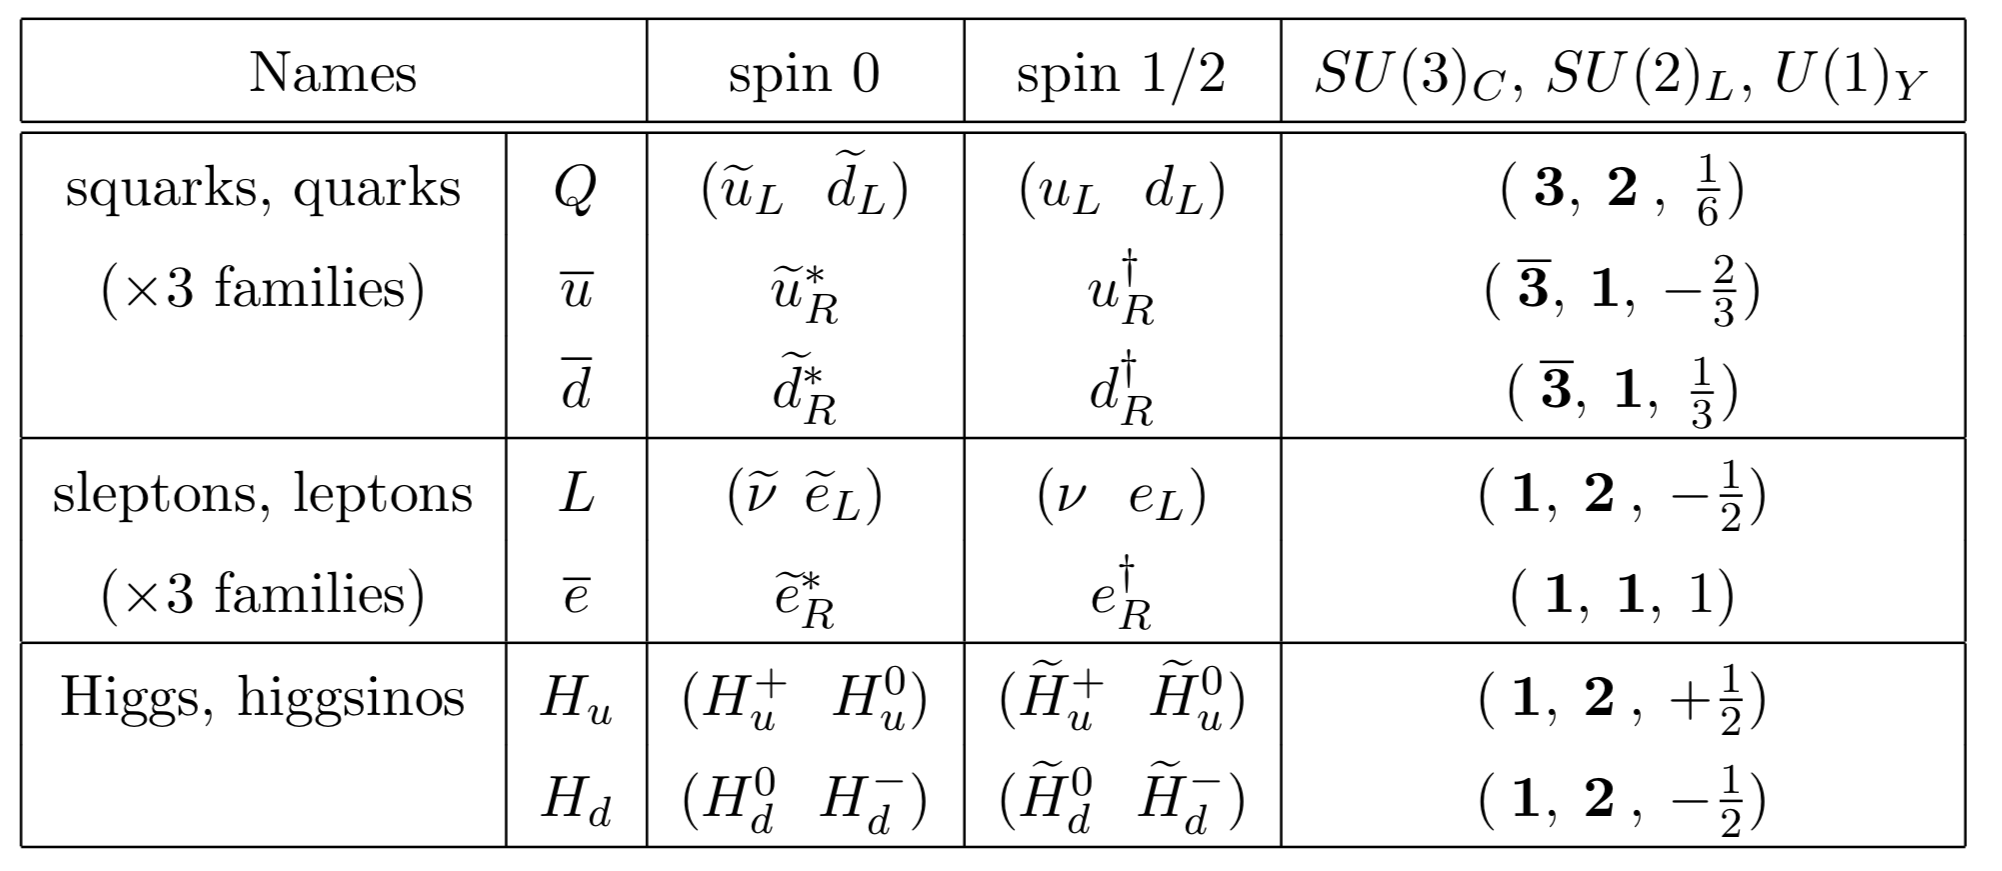
\includegraphics[width=\linewidth]{susy_chiral_superfields}
    \caption{The MSSM chiral superfields, including their names, symbols, and components.
  Quantum numbers for the Standard Model symmetry group transformations are also given~\cite{susy-primer-1998}.}
    \label{tbl:susy_chiral_fields}
\end{table}

\begin{table}[!ht]
    \centering

  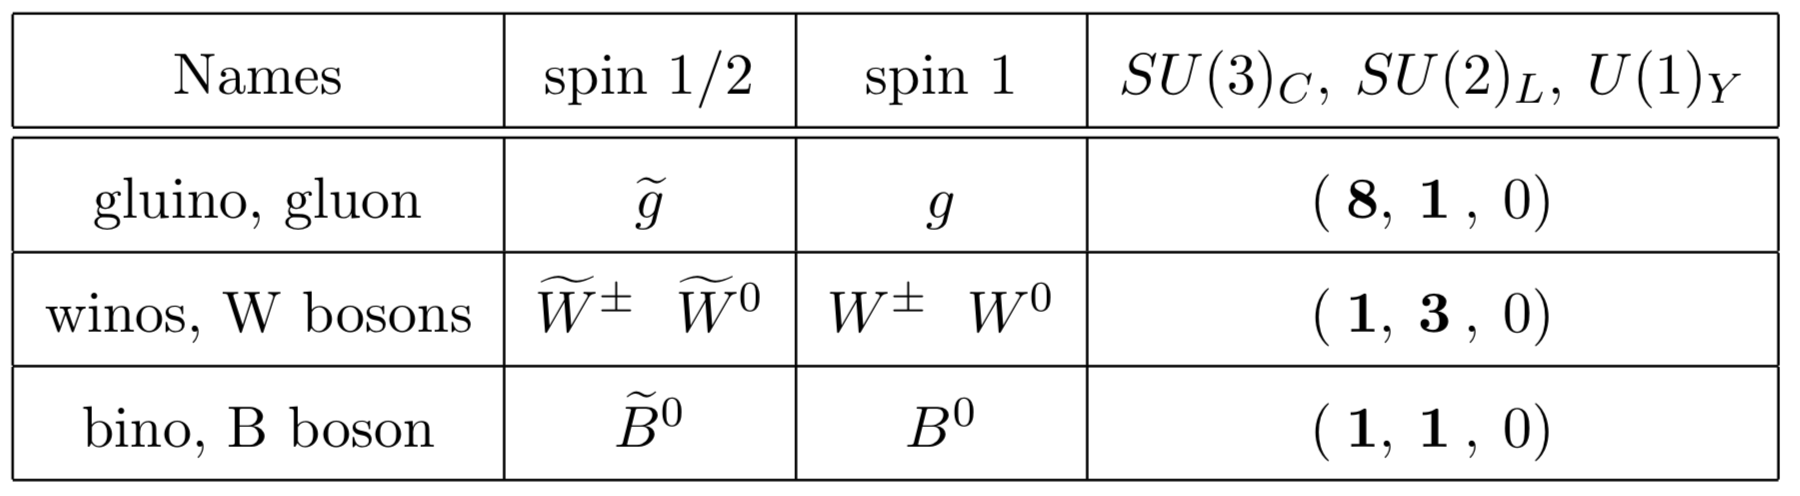
\includegraphics[width=\linewidth]{susy_gauge_superfields}
    \caption{The MSSM gauge superfields, including their names, symbols, and components.
  Quantum numbers for the Standard Model symmetry group transformations are also given~\cite{susy-primer-1998}.}\label{tbl:susy_gauge_fields}
\end{table}
The MSSM superpotential is:
\begin{equation}\label{eq:susy_mssm_superpotential}
    W = h_l^{ij} e_i^c L_j H_d + h_d^{ij} Q_i d_j^c H_d + h_u^{ij} Q_i u_j^c H_u + \mu H_u H_d
\end{equation}
where the indices $i, j, k$ are generation indices.
The superpotential includes all renormalizable terms that preserve the gauge symmetries and are holomorphic in the chiral superfields, except for terms that violate baryon or lepton number conservation.
The superpotential is expressed here only in terms of the left-handed superfields and components.
The hermitian conjugate terms are implied.

\section{R-Parity and R-parity Violation}\label{sec:susy_rpv}

In equation~\ref{eq:susy_mssm_superpotential}, certain terms were excluded from the superpotential because they
violate either baryon number or lepton number conservation.
But this requirement is in fact overly constraining.
While processes that violate baryon number or lepton number conservation have never been observed experimentally,
neither have they been ruled out.
Additionally, while there are no explicit B or L-violating terms in the Standard Model,
and no perturbative process in the Standard Model violates either,
there are in fact non-perturbative effects in the Standard Model which lead to violations of both~\cite{susy-bl-violation}.

\subsection{R-parity}\label{subsec:r_parity}

R-parity is a symmetry which is introduced in order to eliminate the explicit B and L-violating terms from the theory, without have to postulate that B and L are individually conserved.
Each particle has an R-Parity quantum number, defined as:

\begin{equation}\label{eq:r_parity_def}
    P_R = \left(-1\right)^{3\left(B-L\right)+2s}
\end{equation}
where $B$ is the particle's baryon number, $L$ is its lepton number, and $s$ is its spin.
Quarks and squarks carry baryon number $1/3$, leptons an sleptons carry lepton number $1$, and their corresponding antiparticles carry baryon number $-1/3$ and lepton number $-1$.
Every Standard Model particle has $P_R = +1$, and every sparticle has $P_R = -1$.

A necessary consequence of R-Parity conservation is the existence of a stable LSP .
In an R-parity-conserving (RPC) theory, interaction vertices that involve Standard Model particles cannot involve an odd number of sparticles.
As a result, when a sparticle decays, there must be at least one sparticle amongst the decay products, along with any Standard Model particles.
So the lightest sparticle cannot decay, since there is no lighter sparticle for it to decay to.
Furthermore, in RPC SUSY, sparticles can only be produced in pairs at collider experiments, since their production vertices necessarily include Standard Model particles.

\subsection{R-parity violating superpotential terms}\label{subsec:rpv}

If R-Parity conservation is not required, additional terms must be added to the MSSM superpotential.
Each term explicitly violates either baryon number or lepton number by one unit.
These R-Parity-violating (RPV) superpotential terms are:
\begin{equation}\label{eq:rpv_superpotential}
    W_{RPV} = \frac{1}{2} \lambda_{ijk} L_i L_j \bar{e}_k
    + \lambda'^{ijk} L_i Q_j \bar{d}_k + \mu'^i L_i H_u
    + \frac{1}{2} \lambda''^{ijk} \bar{u}_i \bar{d}_j \bar{d}_k
\end{equation}
where $\mu'$, $\lambda$, $\lambda'$, and $\lambda''$ are new coupling constants.
The first three terms result in interaction vertices with $\Delta L = 1$, and the last term has $\Delta B = 1$.

\subsection{Rapid proton decay}\label{subsec:proton_decay}

In general, RPV SUSY would result in proton decay rates far higher than experimental upper bounds.
The main process leading to rapid proton decay requires both the $\lambda'$ and $\lambda''$ terms from equation~\ref{eq:rpv_superpotential}.
In this process, the proton decays to a neutral pion and a positron, via an off-shell squark.
The tree-level diagram leading to such a decay is shown in figure~\ref{fig:susy_proton_decay}
\begin{figure}[!ht]
    \centering
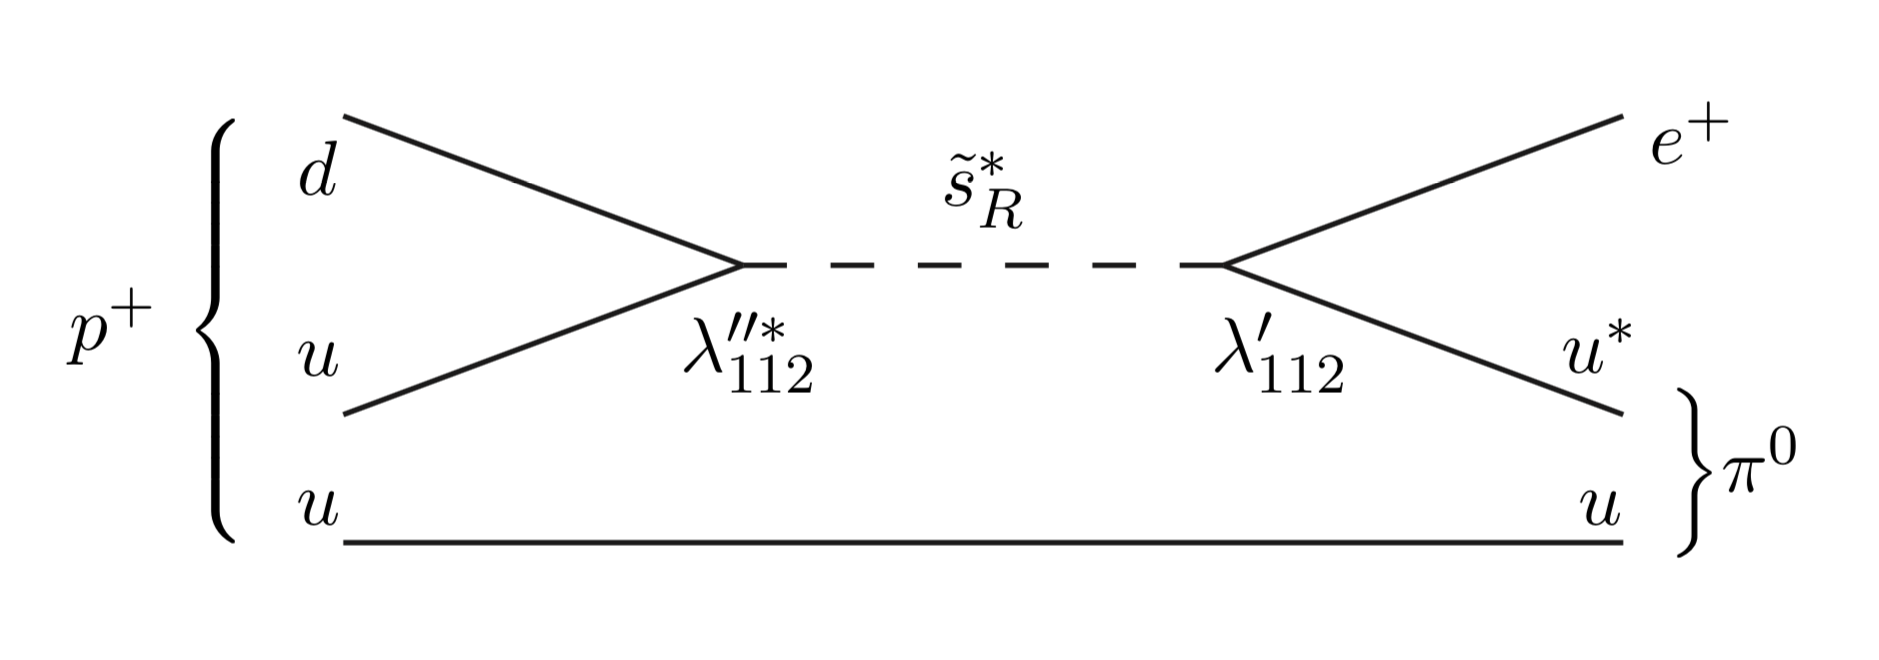
\includegraphics[width=0.95\linewidth]{susy_proton_decay}
\caption{Tree-level diagram for the decay $p^+ \rightarrow \pi^0 e^+$, with both L-violating and B-violating vertices~\cite{susy-primer-1998}.}
\label{fig:susy_proton_decay}
\end{figure}
The tree-level rate for this process is approximately~\cite{susy-primer-1998}:
\begin{equation}\label{eq:proton_decay_rate}
    \Gamma_{p^+ \rightarrow \pi^0 e^+} \sim \frac{m_p^5}{m_{\tilde{d}}^4} \sum_{i=2,3}\left|\lambda'^{11i}\lambda''^{11i}\right|^2
\end{equation}
Experimental bounds on the proton lifetime are greater than $10^{23}$ years,
so in order for RPV SUSY to be consistent with experiment,
either the squark masses have to be extremely large, or one of the couplings $\lambda'$, $\lambda''$ must be extremely small.
Specifically, the coupling and squark masses must satisfy~\cite{susy-rpv-constraints}:
\begin{equation}\label{eq:rpv_constraint}
    \lambda'_{11k} \lambda''_{11k} < 10^{-23} \left(\frac{m_{\tilde{q}}}{100~GeV}\right)^2
\end{equation}
For the search presented here, the ad-hoc assumption that $\lambda' = 0$ is made, in order to prevent predicted proton
decay rates inconsistent with experiment.

\subsection{R-parity violating gluino decays}\label{subsec:rpv_gluino}

The $\lambda''$ RPV term in the superpotential allows for two potential gluino discovery channels at the LHC.
The first involves pair-produced gluinos each decaying to three quarks via an effective vertex with an off-shell squark propagator.
This decay mode will be referred to as the direct decay model.
The second decay mode has the gluino first decaying to two quarks and an on-shell neutralino, via an RPC vertex, and then the neutralino decaying to thre quarks through an effective RPV vertex, which also includes an off-shell squark propagator.
This is the cascade decay model.
Both decay modes result in a large number of high-momentum jets in the event.
Diagrams for these two decay modes are shown in figure~\ref{fig:susy_rpv_decays}.

\begin{figure}[ht!]
    \centering
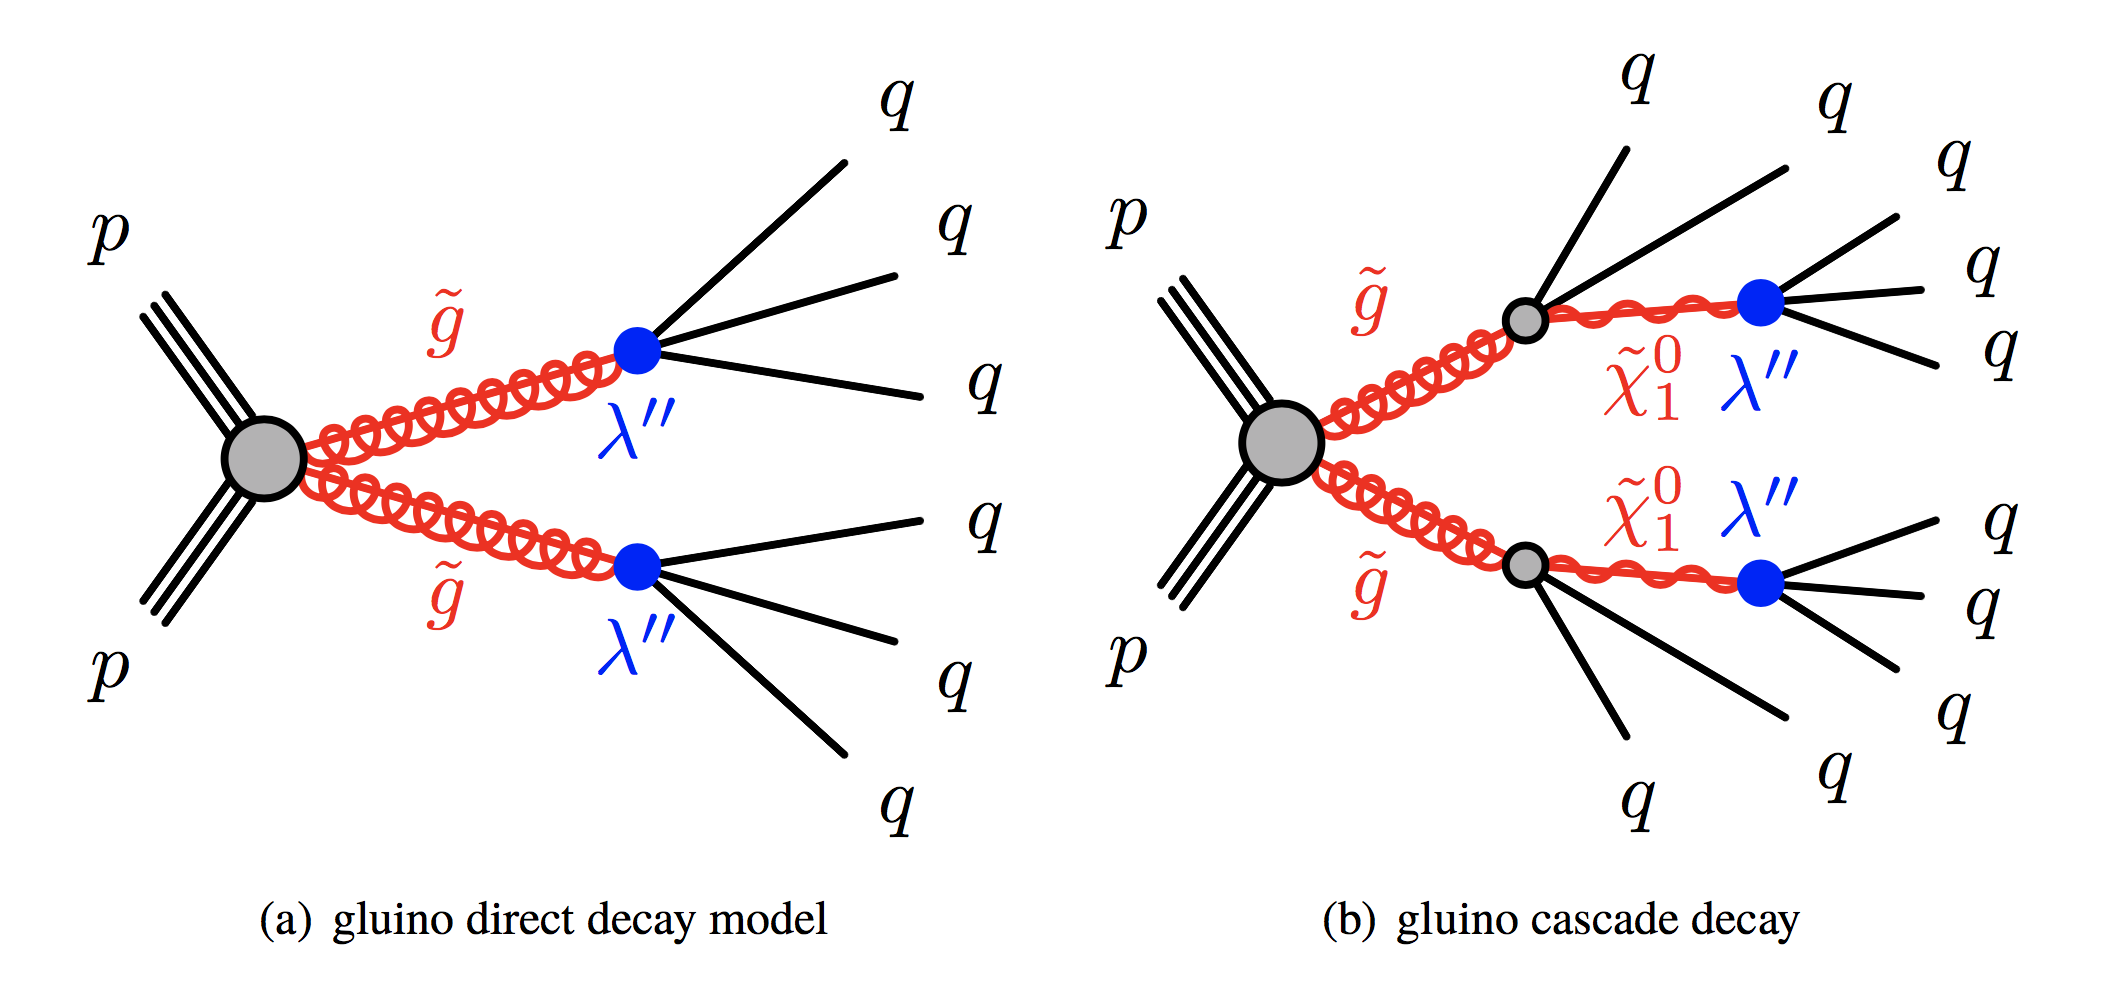
\includegraphics[width=0.95\linewidth]{decay_diagrams_combined}
\caption{Diagrams for the two decay processes that are the subject of this search. The direct decay (left) and cascade decay (right)
both involve effective RPV vertices containing off-shell squark propagators.}
\label{fig:susy_rpv_decays}
\end{figure}
The production and decay rates will depend on the values of the gluino mass, neutralino mass, and $\lambda''$.
A detailed discussion of the signal modeling is presented in chapter~\ref{ch:monte_carlo}.

\chapter{The LHC and ATLAS Detector}\label{ch:atlas}

ATLAS is a system of particle detectors built to measure collisions of both proton-proton and heavy ion collisions
generated by the LHC~\cite{atlas-detector-2008}.
The full detector is $44~m$ long and $25~m$ in diameter.
It consists of an inner detector subsystem for charged particle tracking and electron identification,
electromagnetic and hadronic calorimeters, and a muon spectrometer.

\section{The Large Hadron Collider}\label{sec:lhc}

The Large Hadron Collider (LHC) is the world's largest, highest-energy, highest-luminosity particle accelerator.
It is located inside a $27~km$ circular underground tunnel below the French-Swiss border.
The LHC was designed to produce up to $14~TeV$ center-of-mass energy proton-proton collisions,
as well as lead-ion collisions at a center-of-mass energy of $2.7~TeV/u$.
There are two counter-rotating beams of particles,
which are accelerated to nearly the speed of light and steered into each other at predefined collision points along the
ring, where detectors have been built to measure the particles generated in the collisions.
The highest collision energy achieved to date for proton-proton collisions is $13~TeV$,
with a peak luminosity of $10^{34}~cm^{-2}s^{-1}$~\cite{lhc-guide-2017}.

Collisions generated by the LHC are measured by seven different experiments.
The original four experiments are ATLAS, CMS, LHCb, and ALICE .
ATLAS and CMS are the two general-purpose detectors designed for a variety of measurements and searches for physics
beyond the Standard Model.
They are mainly used to study proton-proton collisions, but are also used for heavy-ion collisions.
LHCb, as the name implies, is a specialized detector built to measure the decays of B mesons.
ALICE is a specialized detector for studying $\mathrm{Pb}-\mathrm{Pb}$ collisions.
In addition to these four experiments, there are three smaller, specialized experiments called TOTEM, LHCf, and MoEDAL .

The LHC is actually the last in a chain of progressively larger accelerators,
each of which adds additional energy to the proton beams until they are injected into the LHC for the final acceleration.
Atoms from a bottle of Hydrogen gas are passed through an electric field to strip their electrons,
resulting in bare protons.
These bare protons are passed into a linear accelerator known as Linac2, which accelerates them to $50~MeV$.
The Proton Synchrotron Booster (PSB) then accelerates the beams to $1.4~GeV$,
before injecting them into the Proton Synchrotron (PS), which accelerates them to $25~GeV$.
The final link in the injection chain before the LHC is the Super Proton Synchrotron,
which accelerates the beams up to $450~GeV$ per proton.
The LHC provides the final boost up to $6.5~TeV$ per proton.
This final stage of acceleration takes approximately 20 minutes, after which the beams can circulate at this energy for
at least 10 hours.

The LHC did not always operate at $13~TeV$.
It took a number of years, over which the energy was increased in steps, before this energy could be reached.
The cumulative luminosity delivered over time each year from 2011 to 2018 is shown in figure~\ref{fig:lhc_lumi_delivered}.

\begin{figure}[!ht]\centering
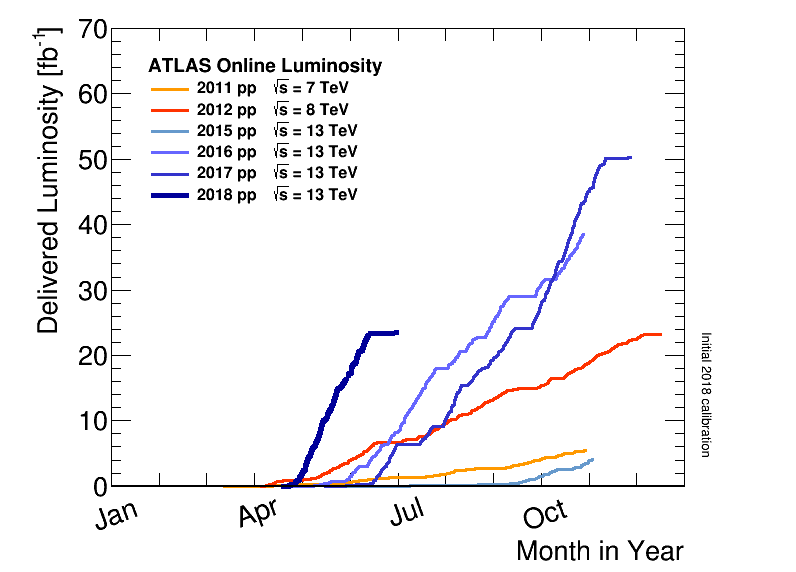
\includegraphics[width=0.9\textwidth]{lhc_lumi_delivered}
\caption{Cumulative luminosity delivered by the LHC over time for each of the years from 2011 to 2018~\cite{lhc-luminosity-public}.}
\label{fig:lhc_lumi_delivered}
\end{figure}

The first two years of data taking, during which the LHC operated at $\sqrt{s}=7~TeV$ and later at $\sqrt{s}=8~TeV$ are known as Run 1.
The first long shutdown (LS1) took place during 2013 and 2014, during which the accelerator was upgraded needed to reach $\sqrt{s}=13~TeV$.
The most time-consuming part of the upgrade involved cycles of cooling and quenching of the superconducting dipole magnets, referred to as "training" the magnets.
The LHC restarted for Run 2 in early 2015, operating at $\sqrt{s}=13~TeV$, with a goal of delivering $150~fb^{-1}$ of proton-proton collision data over a four-year period.
After Run 2, the LHC will be shut down again for 2 years to enable the upgrade to the full $14~TeV$ design energy.
In 2024, it will be shut down again to begin work on the upgrades needed for the high-luminosity LHC (HL-LHC), which aims to increase the instantaneous luminosity by a factor of five~\cite{atlas-hl-lhc}.
Figure~\ref{fig:hl-lhc_plan} shows the planned operation timeline of the LHC from the first collisions in 2011 through to the HL-LHC upgrade in the 2020s.

\begin{figure}[!ht]\centering
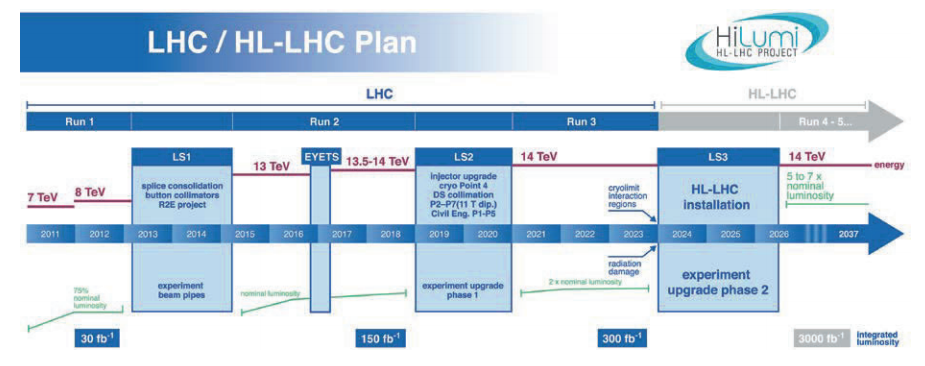
\includegraphics[width=0.9\textwidth]{hl-lhc_plan}
\caption{Planned operation timeline of the LHC, showing the different run periods, shutdown periods, and the energy and luminosity goals, up to and including the HL-LHC upgrades~\cite{atlas-hl-lhc}.}
\label{fig:hl-lhc_plan}
\end{figure}

\subsection{Layout}\label{subsec:lhc_layout}

The LHC was built inside an already existing tunnel,
which originally housed a previous accelerator called the Large Electron-Positron Collider (LEP).
The tunnel is roughly circular and $27~km$ in circumference.
It is buried at an average depth of $100~m$ below ground, sloping at a gradient of $1.4\%$ from its deepest point
of $175~m$ to its shallowest at $50~m$ below ground.

The ring consists of eight arcs and eight straight regions.
The straight regions are referred to as insertions, and the arcs are called sectors.
Octants span from the halfway point of one sector to the halfway point of the next sector, and each contains contain exactly one insertion.
The sectors contain dipole magnets which generate the field needed to bend the beams around the ring.
Four of the insertions are used for particle collisions, where the two beams are focused with quadrupole magnets in order to collide the greatest number of particles in the smallest possible space.
Each of the four main detector experiments are located at one of these insertions.
The other four insertions are used for beam injection, cleaning, and dumping.
Figure~\ref{fig:lhc_layout} shows a schematic of the layout of the LHC, including locations of the four major detector experiments.

There are also three smaller experiments, not shown in the figure, called TOTEM, LHCf, and MoEDAL.
TOTEM and LHCf are specialized for measuring protons and heavy ions emerging from LHC collisions at extremely small angles.
The TOTEM detectors are located close to the interaction point along beamline on either side of the CMS experiment, and LHCf detectors are similarly situated near the ATLAS collision point.
MoEDAL detectors are located within the LHCb insertion, and are designed to search for evidence of magnetic monopoles.

\begin{figure}[!ht]\centering
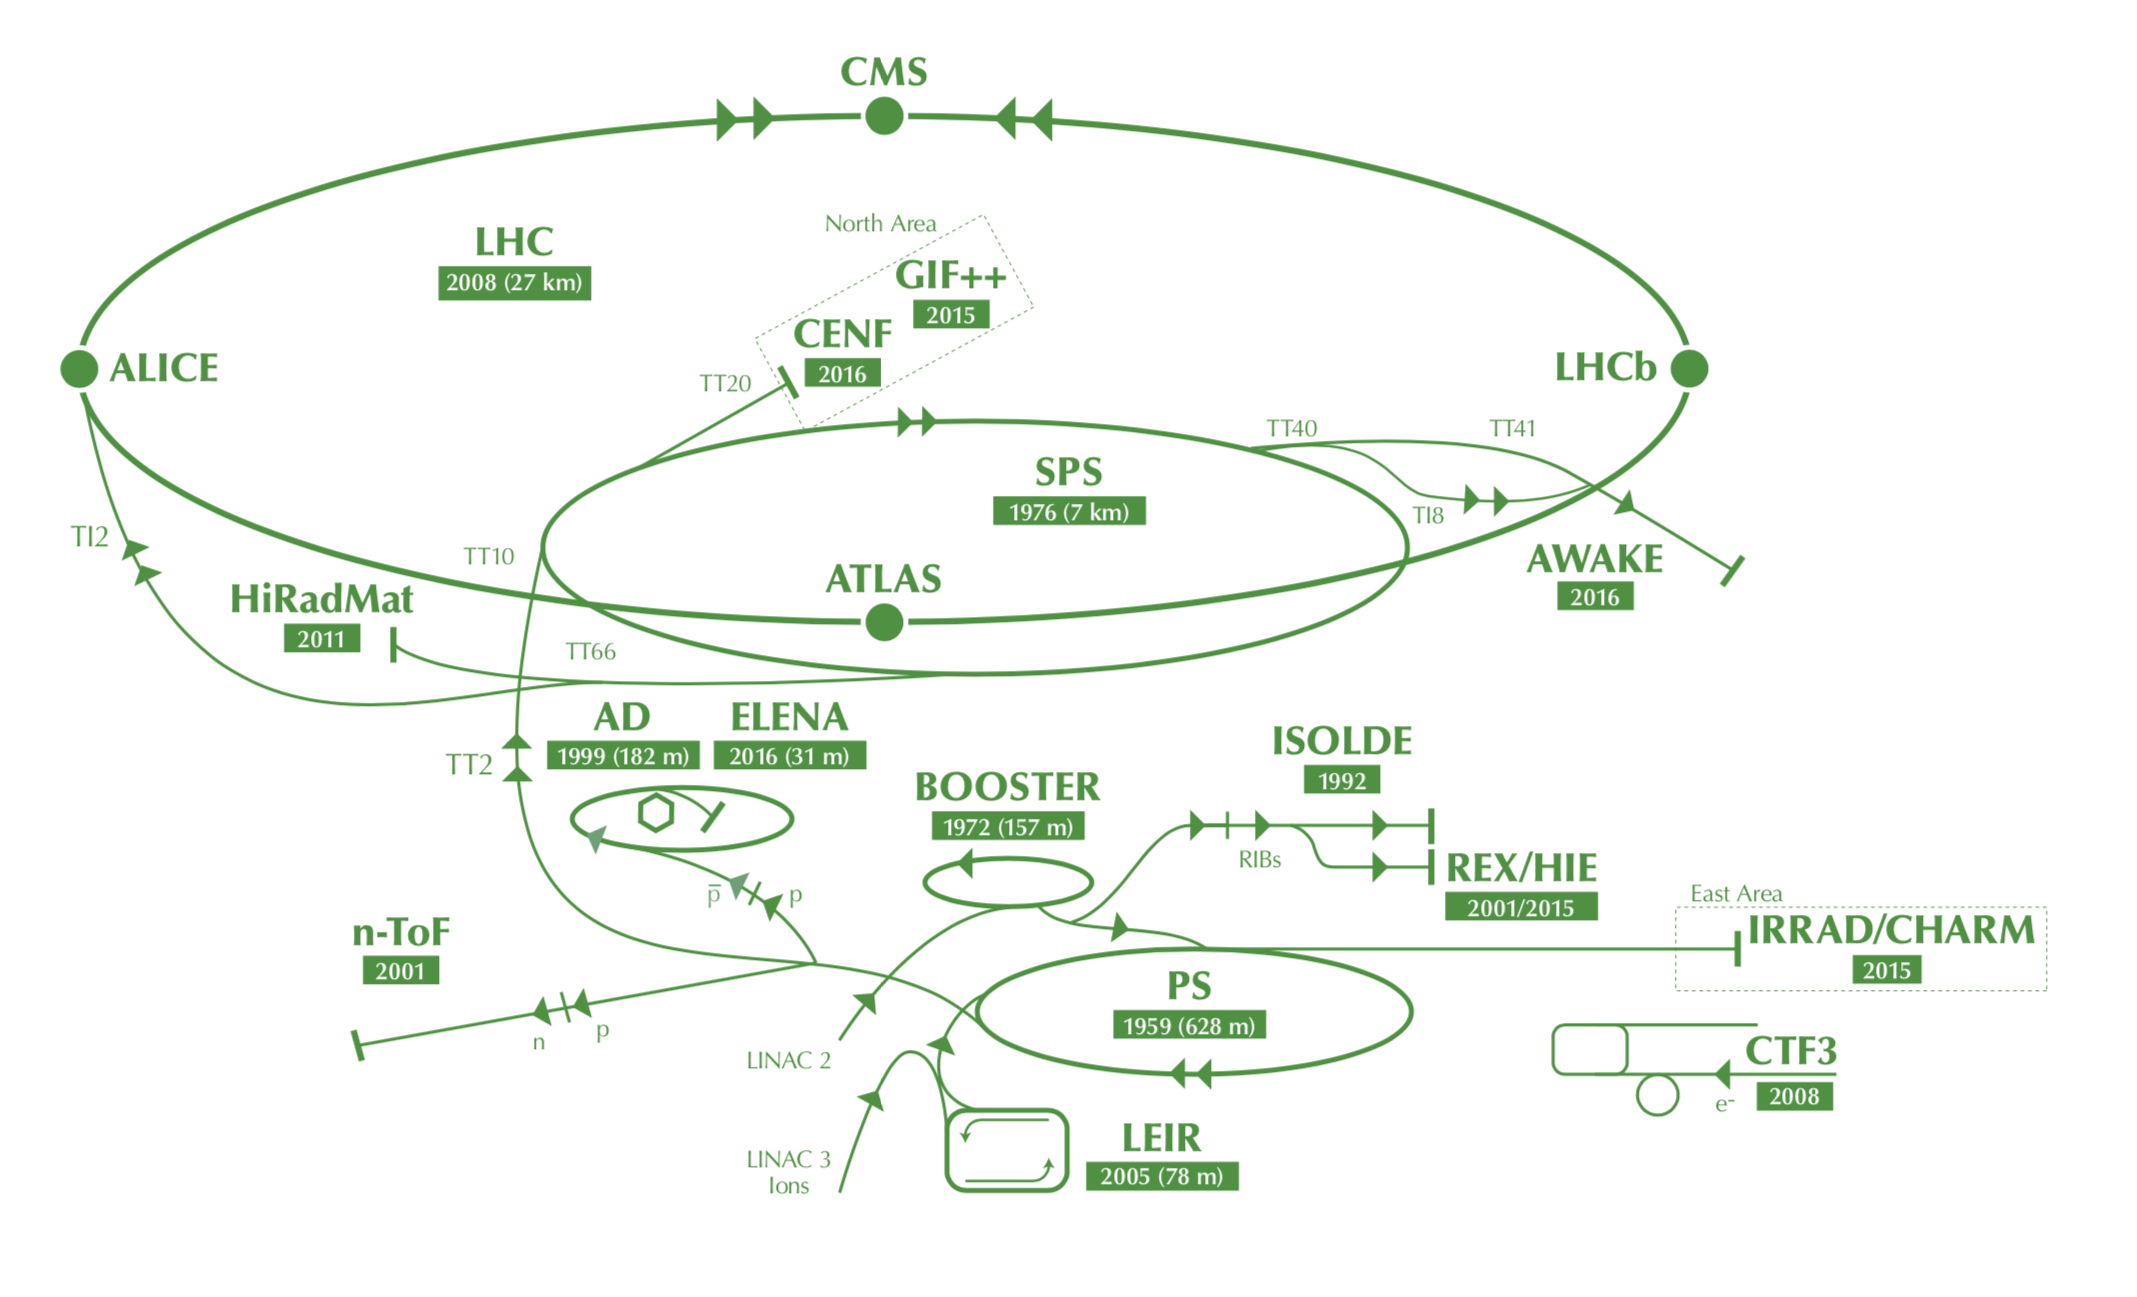
\includegraphics[width=0.9\textwidth]{lhc_layout}
\caption{Schematic of the LHC layout.
The clockwise-rotating beam, shown in red, is referred to as beam 1, and the counter-clockwise-rotating beam, shown in blue, is beam 2.
Locations of the four major detector experiments are labelled~\cite{lhc-machine-2008}.}
\label{fig:lhc_layout}
\end{figure}

\subsection{Magnets}\label{subsec:lhc_magnets}

\subsubsection{Dipoles}
Each of the eight sectors uses 154 dipole magnets to bend the beams around the ring.
All dipole magnets in a sector are connected in series and cooled in the same continuous crystotat.
Each sector is powered independently.
The magnetic field generated by these magnets points in the y-direction
in order to generate a force that points towards the center of the LHC,
according to the Lorentz force law $\vec{F} = q\left(\vec{E}+\vec{v}\times\vec{B}\right)$.

The design and performance of the dipole magnets is crucial to achieving the high energies needed by the LHC physics goals.
This is because the maximum beam energy that can be kept in orbit is proportional to the strength of the magnetic field generated by the dipole magnets.
The dipole magnets are superconducting electromagnets, which generate a field of $8.3~T$.
The superconducting wires are made of $\mathrm{NbTi}$, which has a critical temperature of $10~K$,
but are cooled to and operated at $1.9~K$.
Cooling is done with superfluid helium, which has a very high heat capacity at this temperature.
The wires are made of $7~\mu m$ filaments, thousands of which are twisted together into $15~mm$ strands.
Each cable is then composed of 36 of these strands twisted together.
In order to generate the $8.3~T$ magnetic field, a current of $11.85~kA$ passes through the superconducting wires.
Each dipole magnet is $15~m$ long and weighs $35~\text{tonnes}$.
A schematic of the cross-section of an LHC dipole magnet can be seen in figure~\ref{fig:lhc_dipole}.

\begin{figure}[!ht]\centering
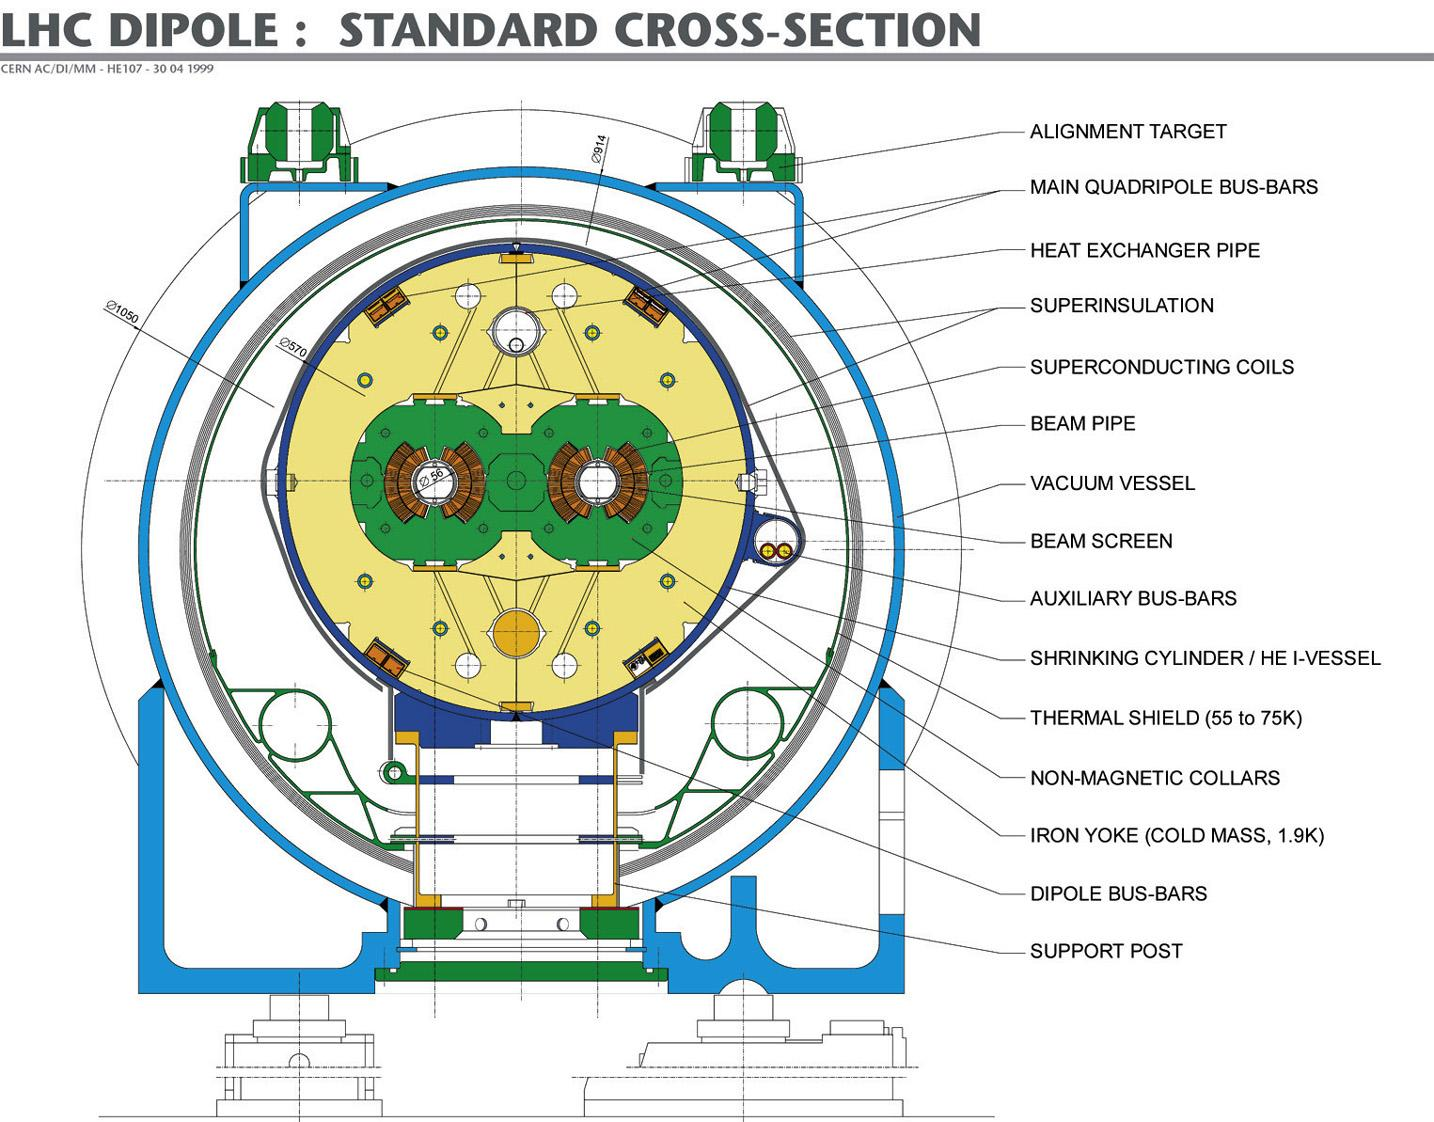
\includegraphics[width=0.9\textwidth]{lhc_dipole}
\caption{Cross-section schematic of an LHC dipole magnet~\cite{lhc-dipole}.}
\label{fig:lhc_dipole}
\end{figure}

\subsubsection{Quadrupoles and higher order}

Quadrupole magnets are located near the interaction points of each detector experiment,
for focusing the beams into the smallest possible area before collisions.
When a beam passes through a quadrupole magnet, it is squeezed along one axis perpendicular to the direction of travel of the beam.
It is simultaneously un-squeezed in the direction perpendicular to both the beam and the squeezing direction,
but the magnitude of the un-squeezing is less than the magnitude of squeezing.
When a beam passes through two successive quadrupole magnets with squeezing directions at 90 degrees to each other,
the net effect is a uniform squeezing of the beam towards its center.
Before entering ATLAS, a series of quadrupole magnets squeezes the beams from approximately $0.2~mm$ to less than $20~\mu m$.
Additional higher-order magnets are used in locations around the LHC for beam corrections and damping of oscillations.
There are also special single-bore dipoles which are used to separate the beams in the region of the RF cavities,
so that separate RF cavities can be used for each beam.

\subsection{Radio frequency cavities}\label{subsec:lhc_rf}

Superconducting radio frequency (RF) cavities, operating at $400~MHz$, and $2~MV$, are used to accelerate and store the beams.
The RF cavities accelerate the beams to their nominal energy,
and continue to supply power over the lifetime of the beams to compensate for energy lost through synchrotron radiation.
There are a total of 16 RF cavities, contained within 4 cryomodules.
Figure~\ref{fig:rf_cryo} is a schematic of an RF cavity cryomodule.

\begin{figure}[!ht]\centering
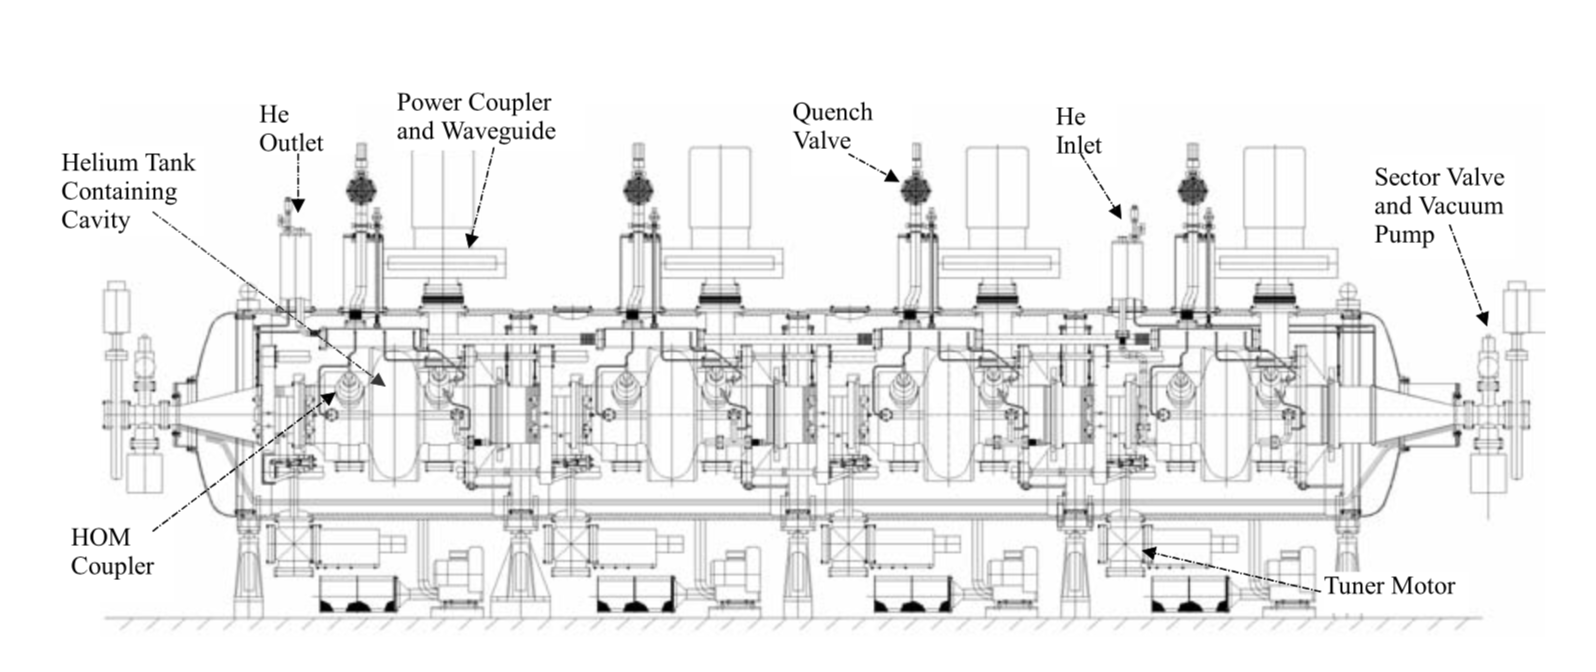
\includegraphics[width=0.9\textwidth]{lhc_rf_cav}
\caption{Schematic of a cryomodule, containing four RF cavities used to accelerate and store the LHC beam~\cite{lhc-machine-2008}.}
\label{fig:rf_cryo}
\end{figure}
The RF cavities are tuned such that the resonant frequency of electromagnetic waves inside the cavity is $400~MHz$.
Protons passing through the cavity will be accelerated or decelerated by the electromagnetic field,
depending on their time of arrival in the cavity.
A proton travelling with the exactly the right energy will enter the cavity with just the right timing to experience zero overall force.
Protons travelling slightly too slowly or too quickly will be decelerated or accelerated until their energy is exactly right.
This process results in protons bunching up around the beam, with all protons traveling at nearly the same $13~TeV$ energy.
The energy spread (rms $\delta p/p$) for the LHC is approximately $1\times 10^{-4}$~\cite{sm-pdg-dark-matter}.

\subsection{Beams and luminosity}\label{subsec:lhc_beam}

Each beam consists of 2,808 bunches of $10^{11}$ protons each.
The frequency of cycles around the LHC is $11,245~Hz$.
Bunches are mostly evenly spaced, with a few gaps that are needed for beam injection or dumping.
Except for the gaps, bunches are spread out to arrive at the collision points every $25~ns$.
When the gaps are taken into account, actual bunches cross with an average frequency of $30~MHz$.
At a luminosity of $7.7\times10^{33}~cm^{-2}s^{-1}$, there will be approximately 40 inelastic collisions per bunch crossing.
Thus the average number of events delivered to ATLAS per second is approximately 1 billion~\cite{lhc-guide-2017}.
Instantaneous luminosity is defined as:
\begin{equation}
\mathcal{L} = \frac{1}{\sigma}\frac{dN}{dt}
\end{equation}
where $\sigma$ is the cross-section of the physics process under consideration, $N$ is the number of events of that type, and $t$ is time.
Luminosity is a property of the accelerator itself, independent of the type of physics process being considered.
It is therefore a useful metric for characterizing the performance of the LHC .

In order to maximize luminosity (and therefore maximize the number of potentially interesting collision events), the most important factor to increase is the number of particles per bunch.
That's because luminosity is proportional to the \textit{square} of the number of particles per bunch, according to~\ref{eq:lumi}.
\begin{equation}\label{eq:lumi}
\mathcal{L} = \frac{N_b^2 n_b f_{rev}}{2\pi \Sigma_x \Sigma_y}
\end{equation}
where $N_b$ is the number of particles per bunch, $n_b$ is the number of bunches per beam, $f_{rev}$ is the frequency of revolutions around the LHC, and $\Sigma_x$, $\Sigma_y$ are the transverse widths of the beam in the x and y direction.
This equation tells us how to maximize instantaneous luminosity: put as many protons as possible into as small a space as possible, and accelerate them as fast as possible.
The peak luminosity delivered to ATLAS by the LHC is $2.06\times10^{34}cm^{-2}s^{-1}$ for proton-proton collisions, and $6.2\times10^{27}cm^{-2}s^{-1}$ for $\mathrm{Pb}$-$\mathrm{Pb}$ collisions.

\section{The ATLAS detector}\label{sec:atlas_detector}
\subsection{Coordinates}\label{subsec:coordinates}
The coordinate system used in this document is the standard ATLAS coordinate system, detailed here.
For both Cartesian and polar coordinates, the origin is defined as the nominal interaction point.
The z-axis points down the beamline.
The x-y plane is perpendicular to the beamline.
The positive y-direction points up, and the positive x-direction points towards the center of the LHC ring.
The positive z-direction therefore points counterclockwise along the LHC, when viewed from above, as required by a right-handed coordinate system.

For cylindrical coordinates, the z-axis is defined the same way as for Cartesian coordinates.
The azimuthal angle $\phi$ is the angle from the positive x-axis, while the polar angle $\theta$ is the angle from the beamline.
A more convenient measure of angle from the beamline is the \textit{rapidity}, because rapidity differences are invariant under Lorentz boosts in the z-direction.
Rapidity is defined as:
\begin{equation}
y = \frac{1}{2}\ln\frac{E+p_z}{E-p_z}
\end{equation}
Another frequently used quantity is the
\textit{pseudorapidity}, which is defined as:
\begin{equation}
\eta = -\ln\frac{\theta}{2}
\end{equation}
Pseudorapidity differences are also invariant with respect to longitudinal Lorentz boosts.
In the limit where $p_T \ll m$, rapidity and pseudorapidity are equal.
Pseudorapidity ranges from zero to plus or minus infinity.
The x-y plane, which is perpendicular to the beamline, is described by a pseudorapidity $\eta=0$.
The z-axis, which is parallel to the beamline, is described by pseudorapidity $\eta=\pm\infty$.

A distance measure in $\eta-\phi$ space is often used, especially when describing jets.
This distance, $\Delta R$ is defined as:
\begin{equation}
\Delta R = \sqrt{\Delta\eta^2+\Delta\phi^2}
\end{equation}

\subsection{Magnet systems}\label{subsec:magnet_systems}
The two ATLAS magnet systems are used to curve the tracks of charged particles passing through the detector,
so that their momenta can be measured. The layout of the magnet systems can be seen in figure~\ref{fig:magnet_layout}.

\begin{figure}[!ht]\centering
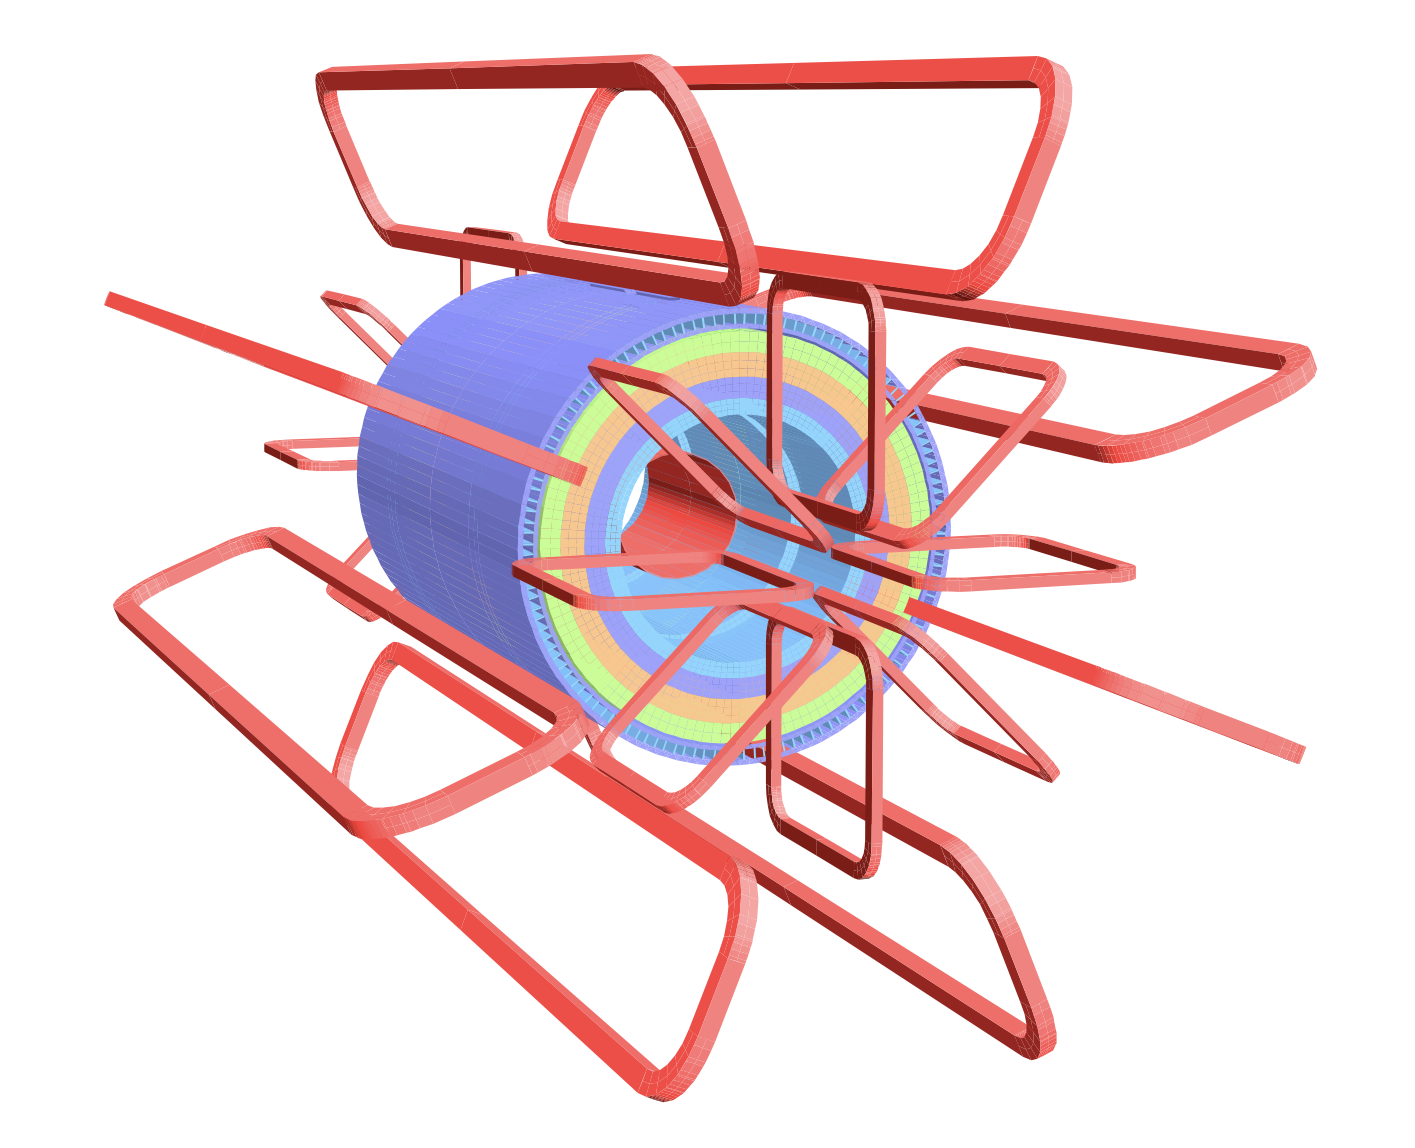
\includegraphics[width=0.9\textwidth]{magnet_layout}
\caption{A diagram showing the layout of the ATLAS magnet system.
The central solenoid is used to apply a force that curves the trajectories of charged particles in the inner detector.
In red are the toroid coils, used to bend the tracks of charged particles passing through the muon spectrometer~\cite{atlas-detector-2008}.}
\label{fig:magnet_layout}
\end{figure}

The first magnetic field is produced by the central solenoid, which surrounds the entire inner detector, and is surrounded by the barrel calorimeters.
It generates a uniform $2~T$ axial magnetic field in the inner detector.
The coils are made of Al-stabilized NbTi. The length is $5.8~m$, and the outer diameter is $2.56~m$~\cite{atlas-detector-2008}.
The second magnet system, used to bend the trajectories of muons passing through the muon spectrometer, has a more complicated geometry.
It consists of a barrel toroid section, and two symmetrical end-cap toroids.
The exact shape of the resulting magnetic field is quite complex, but roughly runs in a circular direction around the calorimeters.

The axial length of the barrel toroid is $25.3~m$, and the outer diameter measures $20.1~m$.
The average field strength is $0.5~T$ and the superconducting material used is similar to that used in the central solenoid\cite{atlas-detector-2008}.
The magnetic field in the region $|\eta|<1.4$ is dominated by the barrel toroid, while the end-cap field dominates the region $1.6 < |\eta| < 2.7$.
The region $1.4 < |\eta| < 1.6$ is the transition region, where both sources contribute significantly to the magnetic field.
Figure~\ref{fig:toroid_end_view} shows an end-on view of the barrel toroid, after installation, and before the calorimeters are inserted.
The end-cap toroids are used to generate the magnetic field for muons passing through the end-cap region of the muon spectrometer.
The properties and geometry of the end-cap toroids are similar to the barrel toroid,
with peak magnetic field reaching $4.1~T$\cite{atlas-detector-2008}.

\begin{figure}[!ht]\centering
\includegraphics[width=0.9\textwidth]{toroid_end_view}
\caption{A picture of the ATLAS barrel toroid after installation.
In the center of the image is the calorimeter and central solenoid, before being moved into the final position~\cite{atlas-detector-2008}.}
\label{fig:toroid_end_view}
\end{figure}

\subsection{Inner detector}\label{subsec:inner_detector}
The inner detector consists of silicon pixel detectors, silicon strip detectors, and transition radiation trackers.
It covers a region from $R = 33~mm$ to $R = 1082~mm$ and $|\eta| = 0$ to $|\eta| = 2.5$.
The layout of inner detector subsystems is shown in figure~\ref{fig:inner_detector_quarter}.

\begin{figure}[!ht]\centering
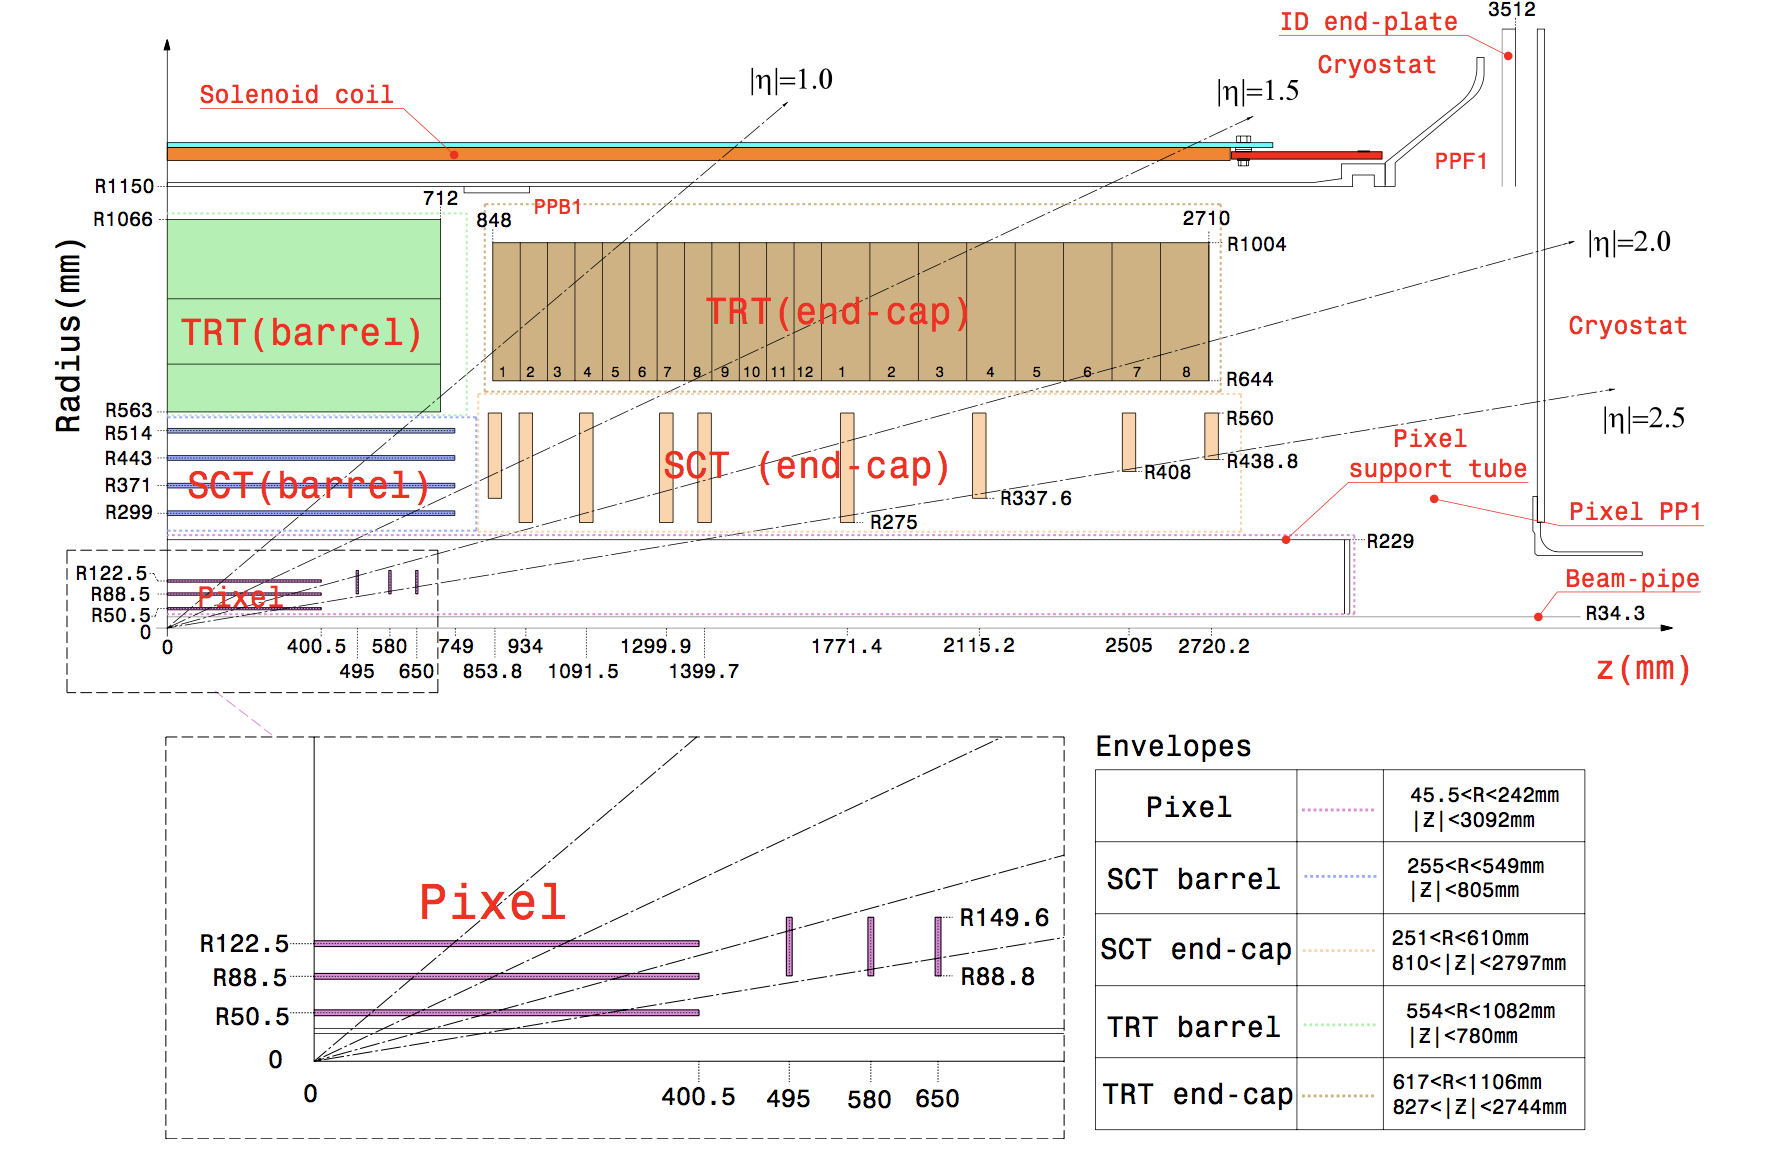
\includegraphics[width=0.9\textwidth]{inner_detector_quarter}
\caption{A quarter-section plan showing the layout of inner detector subsystems and their dimensions.
Not shown is the innermost layer of the pixel detector, the IBL, which was installed in May 2014~\cite{lhc-machine-2008}.}
\label{fig:inner_detector_quarter}
\end{figure}

\subsubsection{Pixel Detector}\label{subsubsec:pixel}

The innermost layer of ATLAS detectors is the pixel system.
Since it lies closest to the interaction point, the pixel system experiences the highest flux of any ATLAS subdetector.
This means that the pixel detector must have the greatest radiation hardness, greatest resolution,
and greatest occupancy of any subdetector~\cite{atlas-detector-2008}.
The pixel system consists of 1744 solid-state pixel sensors, arranged into a barrel region and two endcap regions.
In total, there are 80.4 million pixel readout channels~\cite{atlas-detector-2008}.

The barrel region consists of four concentric cylindrical layers, coaxial with the beamline.
The two endcap regions are each made up of three disks, arranged perpendicular to the beamline.
The pixel barrel envelope covers a region from $z = 0$ to $|z|  = 400.5~mm$.
The four layers are located at increasing distances from the beamline, at $R = 33~mm$, $50.5~mm$, $88.5~mm$, and $122.5~mm$.
The six endcap disks are located at $|z| = 495~mm, 580~mm, 650~mm$ and cover the region $88.8~mm < R < 149.6~mm$~\cite{atlas-detector-2008}.
Figure~\ref{fig:inner_detector_quarter} shows a quarter-section of the entire inner detector, as well as a detailed view of the pixel subsystem, not including the Insertable B Layer (IBL), which was installed in 2014.

The ATLAS pixel sensors are solid-state silicon detectors.
The basic operating principle of a solid-state detector is that charged particles passing through the material generate electron-hole pairs, which are accelerated towards opposite ends of the material via an electric field.
This generates a current, which can be measured by charge-sensitive sensors at the edge of the material~\cite{spieler-2005}.
In a silicon detector, the active material is a pn junction, operated with a reverse bias voltage, until fully depleted.
This reduces the thermal noise from free charge carriers to a low enough level that electron-hole pairs from signal particles can be detected~\cite{spieler-2005}.
In ATLAS, the pixel sensors consist of an n-type bulk, with $p^+$ implants on the back side and $n^+$ implants on the front side.
Before irradiation, the active pn junction region exists between the n-type bulk and $p^+$- implanted side.
Irradiation leads to the reduction in the effective doping concentration, until the bulk material undergoes type inversion.
After type inversion, the active pn junction region switches to the $n^+$-doped side~\cite{pixels-2008}.
This process is illustrated in figure~\ref{fig:pixel_type_inversion}.
This $n^+$-in-$n$ design allows the sensors to continue to operate both before and after large doses of radiation.
Each pixel tile has 47232 pixels, laid out in a grid of 144 columns by 328 rows.
Some of the pixels are grouped to common read-out channels, resulting in 46080 read-out channels.
This grouping is done so that an equal number of read-out channels can be connected to each of the 16 front-end read-out chips~\cite{pixels-2008}.
In 128 of the columns, each pixel implant is $382.5\times30~\mu m^2$, with pitch (center-to-center distance) of  $400\times50~\mu m^2$.
In the remaining 16 columns, the pixel sizes are $582.5\times30~\mu m^2$, with a pitch of  $600\times50~\mu m^2$~\cite{pixels-2008}.

\begin{figure}[!ht]\centering
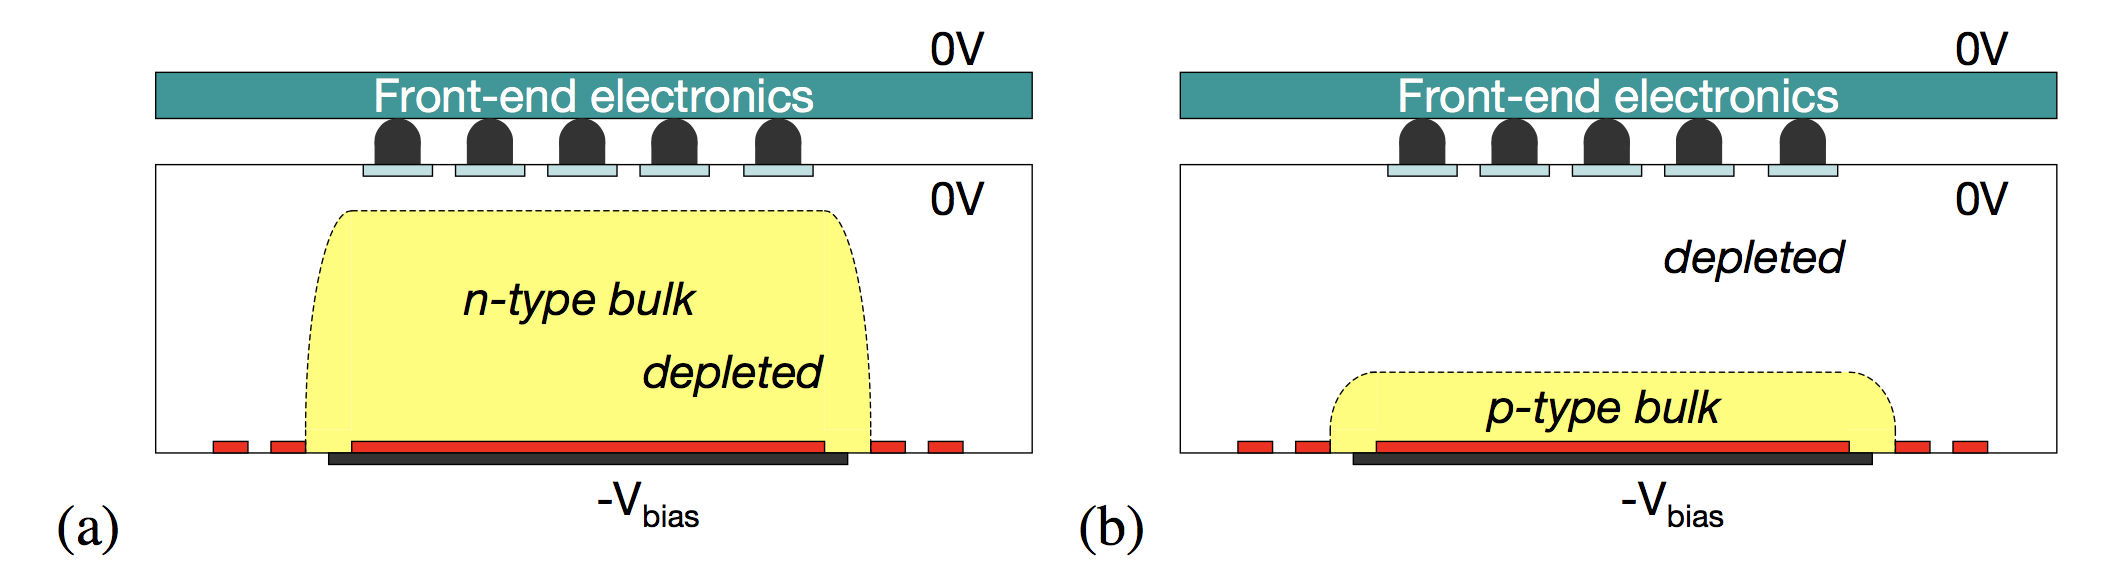
\includegraphics[width=\textwidth]{pixel_type_inversion}
\caption{Graphic illustrating how $n^+$-in-$n$ pixel sensors continue to operate after the type inversion that results from irradiation.
In (a), the unirradiated state, the bulk is n-type, and the depletion zone occurs between the $p^+$-doped back side.
After type inversion, in (b), the depletion zone occurs between the now p-type bulk and the $n^+$-doped front side~\cite{pixels-2008}.}
\label{fig:pixel_type_inversion}
\end{figure}

A major upgrade that occurred during the long shutdown in 2014 was to install the Insertable B-Layer (IBL) to the pixel detector.
The IBL became the fourth and innermost layer of the pixel detector.
It provides several key improvements to the tracking system, which will allow the pixel detector to maintain good performance even in the higher-luminosity environment that will be present in the High Luminosity LHC (HL-LHC)~\cite{ibl-tdr}.
The IBL does this by improving tracking robustness against module failures, adding measurement redundancy to mitigate the effects of pileup, and adding an additional measurement closer to the interaction point~\cite{ibl-tdr}.
As part of the IBL insertion project, the original beam pipe was removed, and replaced with a smaller-radius beampipe.
Precision tooling and methods for insertion were developed and practiced for two years before the procedure was finally carried out.
The tolerances were extremely tight, with only a $0.2~mm$ gap between the IBL and inner supporting tube~\cite{ibl-website}.
An image of the IBL being inserted can be seen in figure~\ref{fig:ibl_insertion}

\begin{figure}[!ht]\centering
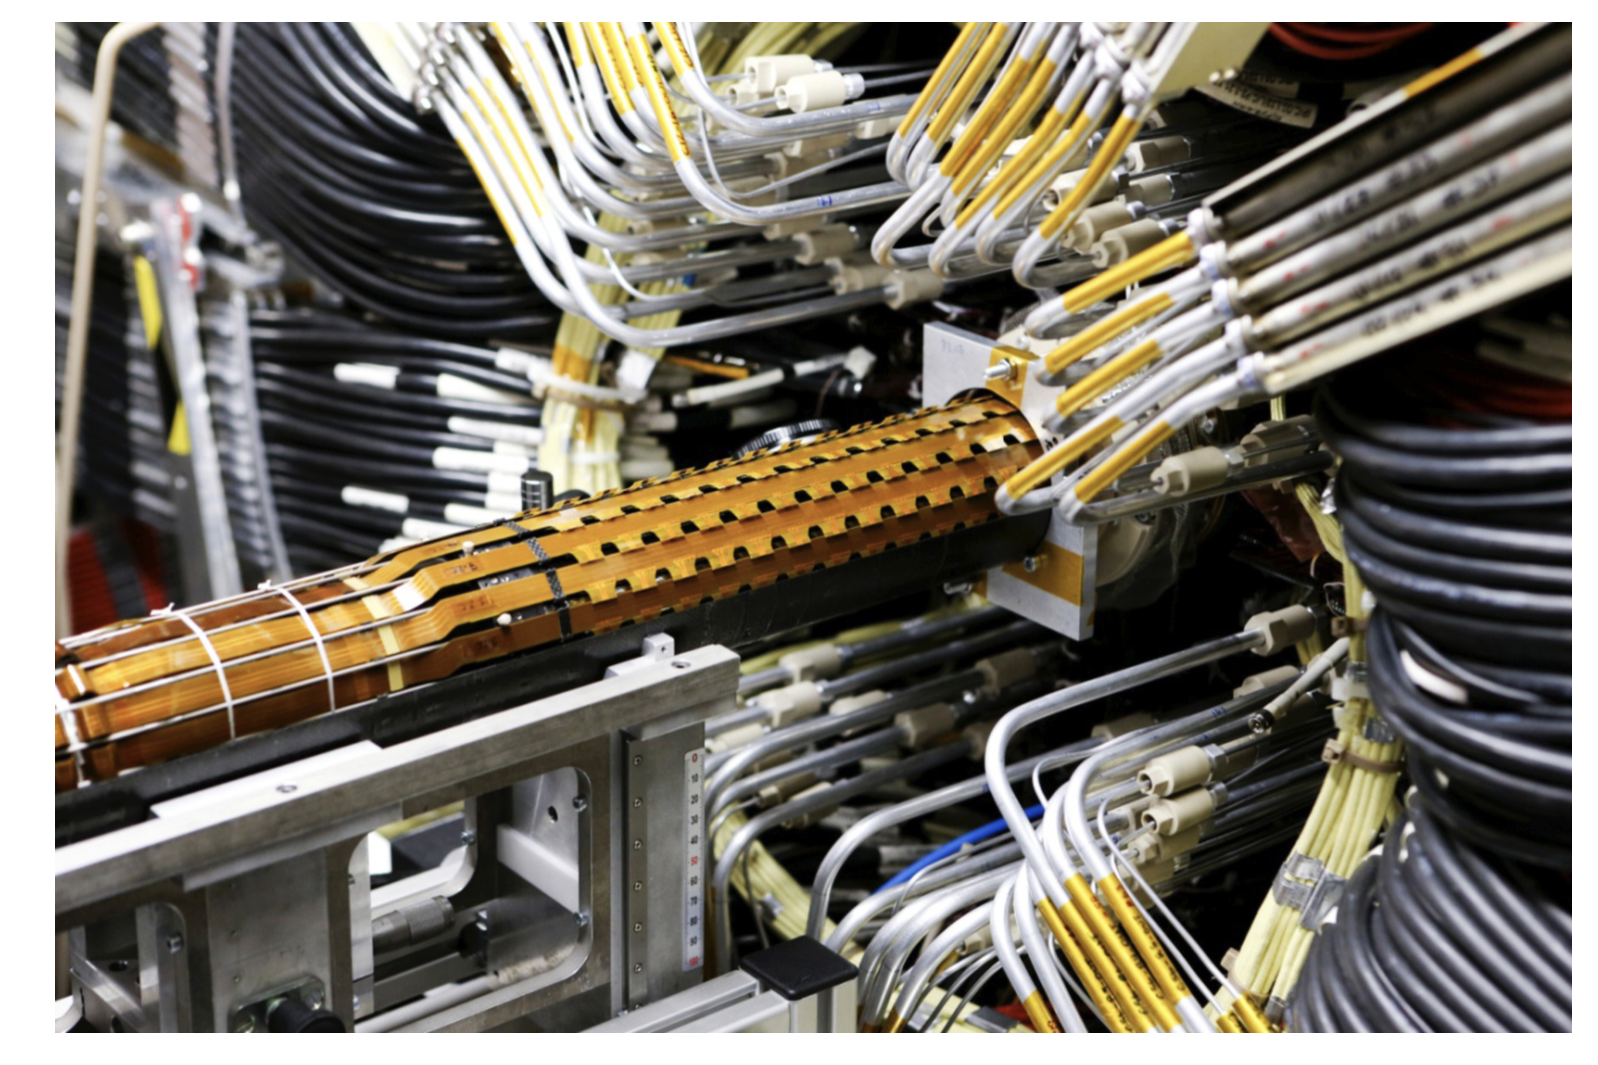
\includegraphics[width=0.9\textwidth]{ibl_insertion}
\caption{The IBL as it was inserted into the pixel detector~\cite{ibl-website}.}
\label{fig:ibl_insertion}
\end{figure}

\subsubsection{Silicon Strip Tracker}\label{subsubsec:sct}

After the pixel detector system, the next innermost subdetector is the SemiConductor Tracker, or SCT .
The SCT consists of 4088 modules, with a total silicon surface area of $63~m^2$~\cite{atlas-detector-2008}.
Like the pixel system, the SCT barrel region consists of four concentric cylindrical layers, coaxial with the beamline.
The two endcap regions are each made up of nine disks, arranged perpendicular to the beamline.
The SCT barrel envelope covers a region from $z = 0$ to $|z|  = 746~mm$, and the four layers are located at increasing distances from the beamline, at $R = 299~mm$, $371~mm$, $443~mm$, and $514~mm$~\cite{sct-barrel-2006}.
The nine endcap disks on each side range from $|z| = ~mm$ to $|z| = ~mm$, and cover the region $275~mm < R < 560~mm$~\cite{atlas-detector-2008}.

Like in the pixel system, the SCT sensors are solid-state silicon detectors.
Instead of pixels, the base unit is a strip of silicon, ranging in length from $6$ to $13~cm$.
The modules are arranged in back-to-back pairs at a stereo angle of $40~mrad$, in order to provide two-dimensional resolution.
These strips are made of p-type silicon, and are embedded in n-type silicon.
The average pitch is $80~\mu m$~\cite{sct-2010}.
The resolution resulting from this design is $17~\mu m$ in the $r-\phi$ direction, and $580~\mu m$ in the z-direction~\cite{sct-2010}.

\subsubsection{Transition Radiation Tracker}\label{subsubsec:trt}
Moving outwards from the pixel system and SCT, the final inner detector subsystem is the transition radiation tracker, or TRT .
Unlike the pixel or SCT systems, the TRT uses proportional drift tubes, referred to as straws, as sensors.
To make accurate track measurements, the TRT relies on a larger number of hits over a longer distance than the pixel system or SCT .
Since the TRT measures approximately 36 hits per track, and makes measurements over a longer distance, less spatial precision is required per hit~\cite{atlas-detector-2008}.
The TRT only provides tracking information in the $R-\phi$ direction, unlike the pixel and SCT systems, which each provide three-dimensional tracking information.
The main purpose of the TRT is to provide additional tracking information.
But transition radiation photons generated in the TRT gas-filled tubes can also aid in electron identification~\cite{atlas-detector-2008}.

The TRT uses proportional drift tubes to detect charged particles.
A tube is filled with a mixture of two or more gases, including an inert gas such as Xenon, and an electric field is applied across the tube.
When a charged particle passes through the tube, ion pairs are generated from the inert gas.
Positive and negative ions drift in opposite directions, towards the cathode and anode, respectively.
If a particle's energy is completely absorbed in the tube, the number of ions produced in stopping the particle is proportional to the original energy of the particle~\cite{knoll-2000}.
In addition to the inert gas, it is common to add another gas, such as Carbon Dioxide, to stabilize the ionization process.
This additional gas is referred to as a quencher gas.

Like the pixel system and SCT systems, the TRT consists of a barrel region and two end-cap regions.
In the barrel region, straw tubes are arranged coaxial to the beamline and measure $144~cm$ in length.
In the end-cap region, straw tubes are arranged radially, and measure $37~cm$ in length~\cite{atlas-detector-2008}.
The TRT barrel envelope covers a region from $z = 0$ to $|z|  = 780~mm$, and $554 < R 1082~mm$, and the end-cap envelop covers a region from $z = 848$ to $|z|  = 2710~mm$, and $644 < R 1004~mm$.
This provides tracking coverage out to $|\eta| = 2.0$~\cite{atlas-detector-2008}.
A charged track passing trough the TRT will typically produce 36 hits.
Each straw provides a hit resolution of $130~\mu m$.
The TRT has a total 351,000 total readout channels.

\begin{figure}[!ht]\centering
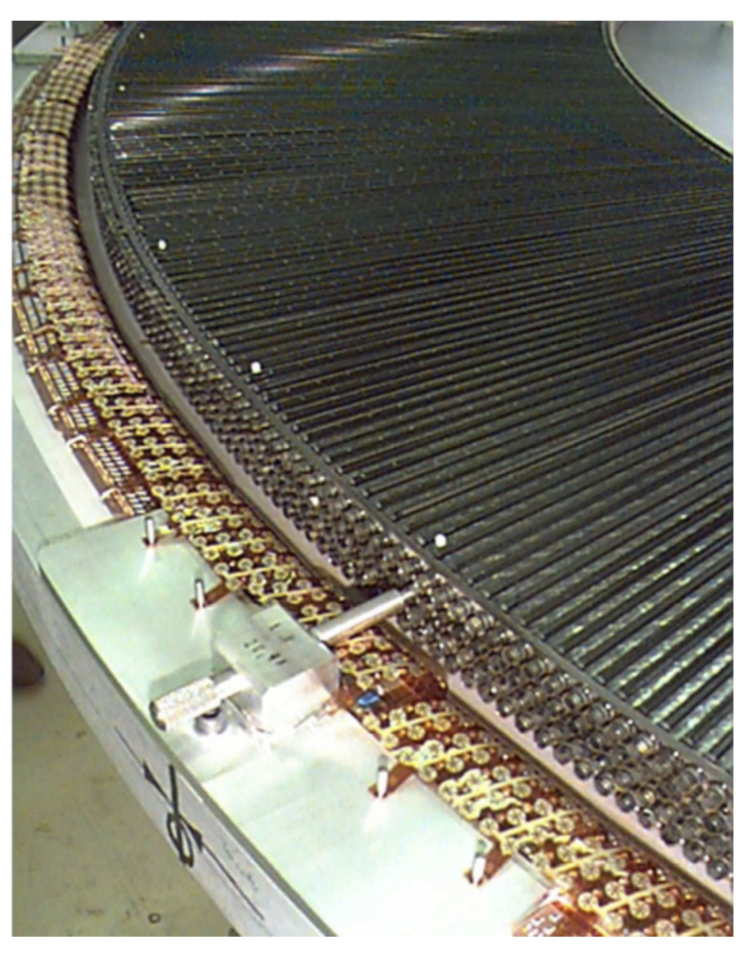
\includegraphics[width=0.4\textwidth]{trt_end_cap}
\caption{Part of a TRT end-cap, showing the radial layout of the $37~cm$ straw tubes~\cite{trt-2013}.}
\label{fig:trt_end_cap}
\end{figure}

The TRT straw tube walls are constructed of two layers of $25~\mu m$-thick Kapton film.
The Kapton is coated with a $0.2~\mu m$-thich layer of aluminum, followed by a $6~\mu m$-thich layer of carbon-polyimide.
The Aluminum layer serves to provide electrical conductivity, and the carbon-polyimide layer is to protect the aluminum.
The two Kapton layers are sealed together with a $5~\mu m$-thick polyurethane layer~\cite{trt-2013}.
The TRT straw wall design is shown in figure~\ref{fig:trt_straw_wall}

\begin{figure}[!ht]\centering
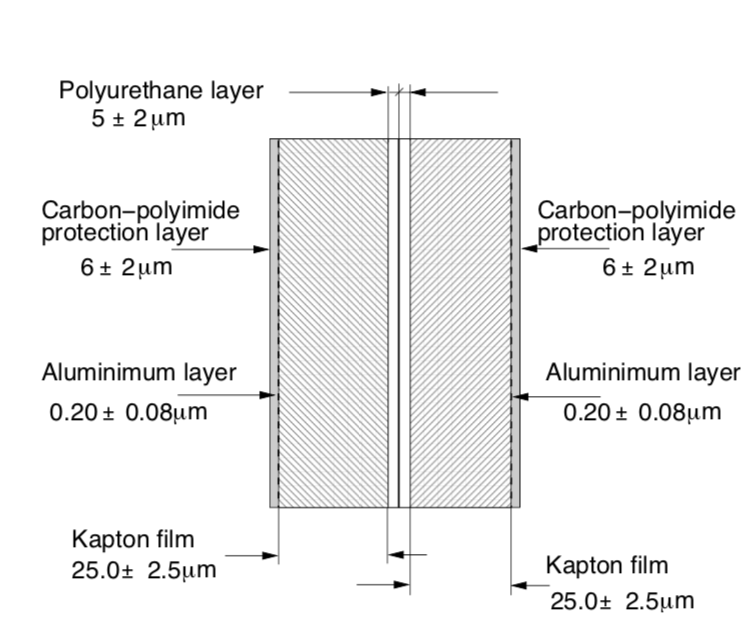
\includegraphics[width=0.9\textwidth]{trt_straw_wall}
\caption{Schematic of the TRT straw wall design. Two coated Kapton layers are sealed together with polyurethane~\cite{trt-2013}.}
\label{fig:trt_straw_wall}
\end{figure}

The straws are filled with a mixture of $70\%~\mathrm{Xe}$, $27\%~\mathrm{CO_2}$, and $3\%~\mathrm{O_2}$.
Carbon dioxide is used as a quencher gas, which is needed to guarantee that the ionization procedure is stable.
The addition of a small amount of oxygen increases the voltage difference between the working point and the breakdown voltage, further stabilizing the process~\cite{trt-2013}.

In order to maximize hit efficiency, the straw diameter should be as large as possible.
But there is a tradeoff: as straw diameter increases, so does the drift time.
The optimal diameter to ensure acceptable time resolution for $25~ns$ bunch-spacing was determined to be $4~cm$~\cite{trt-2013}.

\subsubsection{Tracking Resolution}
The number of layers crossed per track and the intrinsic accuracy for each inner detector subsystem is summarized in table~\ref{tbl:track_resolution}.
The TRT provides the largest number of hits per track, but has the poorest resolution, and only provides resolution in $R-\phi$.
The Pixel and SCT systems have much better resolution in $R-\phi$ and also provide $z$-resolution in the barrel region, and $R$-resolution in the disks.
\begin{table}[!ht]\centering
\begin{tabular}{cccc}
    \toprule
          & number of layers & $R-\phi$ resolution & $z$ resolution (barrel) / $R$ resolution (disks) \\ \midrule
    Pixel & 3                & $10~\mu m$          & $115~\mu m$ \\
    SCT   & 8                & $17~\mu m$          & $580~\mu m$ \\
    TRT   & 36               & $130~\mu m$         & N/A \\ \bottomrule
\end{tabular}
\caption{Summary of number of layers crossed per track as well as intrinsic accuracy in $R-\phi$ and $z$ for each of the inner detector subsystems.}
\label{tbl:track_resolution}
\end{table}

\subsection{Calorimeters}\label{subsec:calorimeters}

The ATLAS calorimeters are designed to absorb and measure the energy of both electromagnetic and hadronic showers.
Different materials and geometries are used for different calorimeter subsystems, but the operating principle is the same.
In each calorimeter, there is an absorber medium, and a sampling medium.
When a particle strikes the absorber medium, it triggers a shower of particles which then pass into the sampling medium.
The sampling medium is ionized by these showering particles, and instrumentation is used to measure the amount of ionization.
In order to accurately measure shower energy, the ATLAS calorimeters are designed to fully absorb both electromagnetic and hadronic showers.

The innermost calorimeter is a high-granularity detector optimized for measuring electromagnetic showers, which covers the range $|\eta| < 3.2$.
In the electromagnetic calorimeter, lead is used as an absorber and LAr as the sampling medium.
The outer calorimeter has a coarser granularity and is optimized for measuring jets and $E_{T miss}$ .
It consists of scintillator tiles and uses steel as the absorber.
In addition to the EM and hadronic calorimeters, there is copper-tungsten/LAr calorimeter providing coverage out to $|\eta| < 4.9$, known as the forward calorimeter, or FCal.
The layout of the full ATLAS calorimeter system can be seen in figure~\ref{fig:calo_full}

\begin{figure}[!ht]\centering
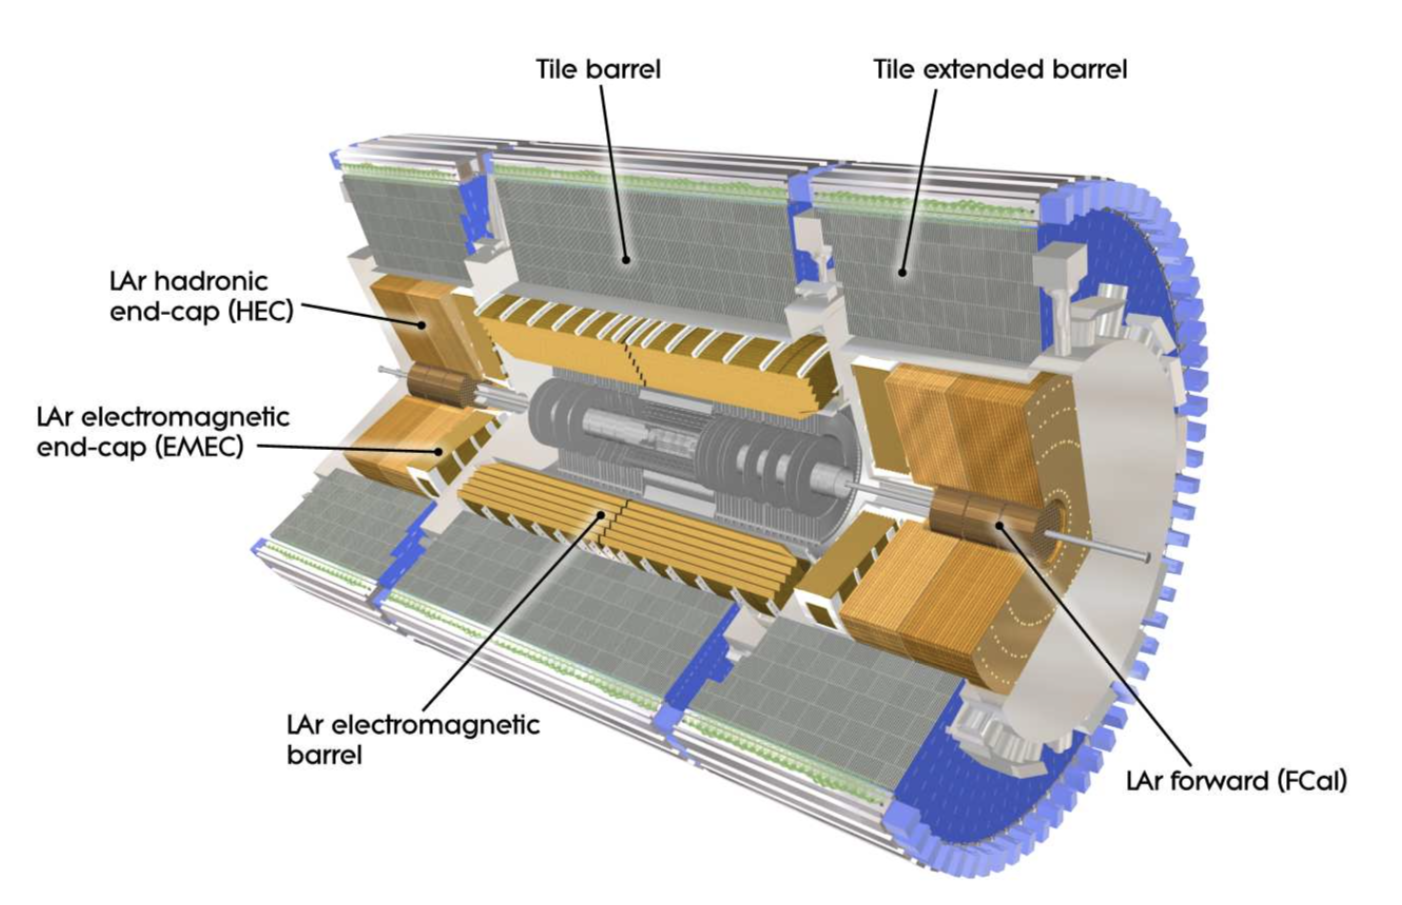
\includegraphics[width=0.9\textwidth]{calo_full}
\caption{Layout of the ATLAS calorimeter system~\cite{atlas-detector-2008}.}
\label{fig:calo_full}
\end{figure}

\subsubsection{Electromagnetic Calorimeters}\label{subsubsec:em_cal}

The electromagnetic calorimeter is located just outside the solenoid that surrounds the inner detector.
It is optimized for measuring the energy of electromagnetic showers.
The EM calorimeter is also designed to measure the direction of neutral particles, which cannot be tracked by the inner detector.
In the barrel region, the EM calorimeter covers the range $|\eta| < 1.475$.
In the end-cap region, it covers a range of $1.375 < |eta| < 3.2$.

The calorimeters have to be thick enough to fully absorb shower energy and to minimize punch-through into the muon system.
The EM calorimeter depth was designed to be 22 interaction lengths $\left(X_0\right)$ in the barrel, and $24~X_0$ in the end-caps.
An interaction length is defined as the average distance traveled by a particle through a material when it has lost
$1 - 1/\mathrm{e}$ of its original energy~\cite{em-calo}.

The calorimeters consist of accordion-shaped lead absorber plates with copper-kapton electrodes in between.
The accordion shape provides full symmetry in $|\phi|$ with no gaps.
The absorber plates are grounded and the electrodes are kept at $2000~V$ in the barrel region and between
$1000$ and $2500~V$ in the end-cap region.
The whole system is immersed in liquid argon~\cite{atlas-detector-2008}.
A particle passing through the lead absorbers generates a shower of particles, which ionize the LAr.
Due to the electric field between the absorber plates and electrodes, ions drift towards the electrodes.
This generates a pulse in the electrodes which can then be recorded.

The calorimeter cells are arranged into three layers, with highest granularity closest to the interaction point.
Cells in layer 1 have a granularity of $\delta\phi \times \delta\eta = 0.0245 \times 0.0031$.
This very fine segmentation is useful in accurately determining the direction of incoming particles.
It is also useful in discriminating between an individual photons and a neutral $\pi$ meson decaying to two photons~\cite{em-calo}.
In the second layer, the granularity is reduced $\delta\phi \times \delta\eta = 0.0245 \times 0.025$.
In the third and final layer, the granularity is further reduced to $\delta\phi \times \delta\eta = 0.0245 \times 0.05$.
The geometry of the EM calorimeter cells can be seen in figure~\ref{fig:em_calo}

Inside the innermost layer of the barrel EM calorimeter is an $11~mm$-thin presampler, covering a range of $|\eta| < 1.8$.
The purpose of this presampler is to correct for energy lost to material upstream of the EM calorimeter.

\begin{figure}[!ht]\centering
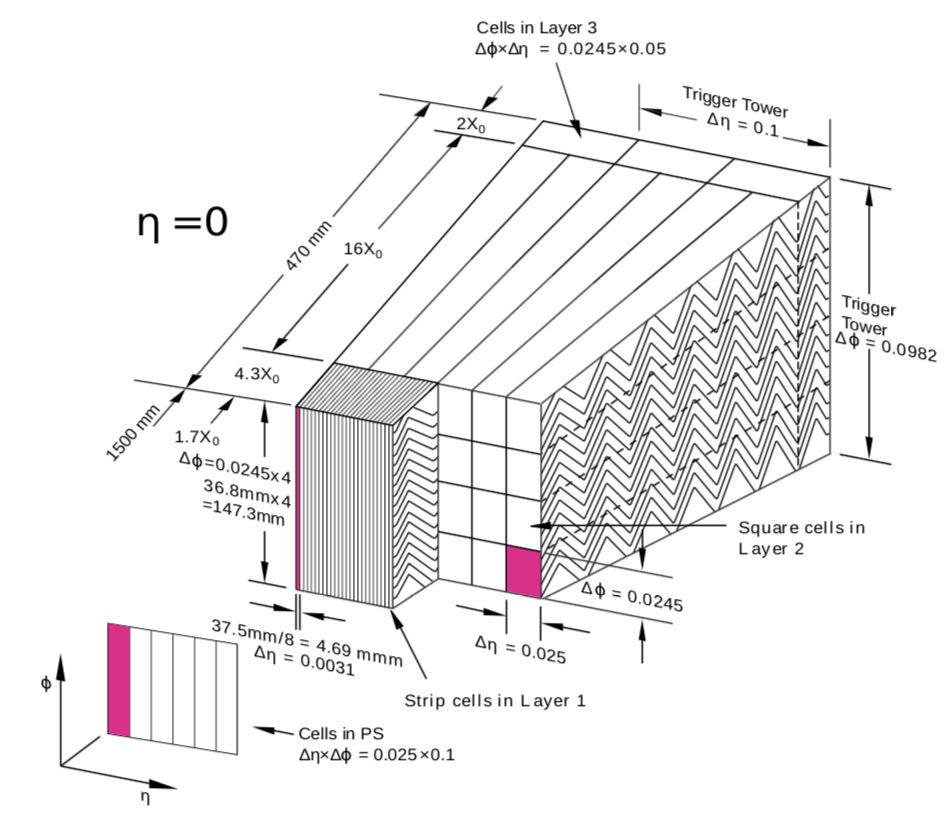
\includegraphics[width=0.6\textwidth]{em_calo}
\caption{Schematic of EM calorimeter, showing the granularity of each layer~\cite{em-calo}.}
\label{fig:em_calo}
\end{figure}

\subsubsection{Hadronic Calorimeters}\label{subsubsec:had_cal}

The most important ATLAS subdetector for measuring jets is the hadronic calorimeter system.
The hadronic calorimeter system consists of central and extended tile calorimeter barrels, two end cap calorimeters, and a forward calorimeter.

The central tile barrel covers the range $|\eta|<1.0$, the extended tile barrels cover the range $0.8 < |\eta| < 1.7$, and the end-cap calorimeters cover the range $1.5 < |\eta| < 3.2$.
The forward calorimeters (FCal) cover the extreme forward region, $3.1 < |\eta| < 4.9$.
The central barrel is $5.8~m$ long, and the extended barrels are each $2.6~m$ long.
Both the central and extended barrels cover the range $2.28~m < R < 4.25~m$.
Each of the three tile calorimeters is composed of 64 wedge-shaped modules.
The geometry of the hadronic calorimeter system, not including the end-caps, can be seen in figure~\ref{fig:calo_full}.

The hadronic calorimeters in the central and extended barrel regions are tile calorimeters, which consist of alternating steel absorber plates and scintillating tiles.
Particles that pass through the steel plates generate hadronic showers.
The hadrons from these showers then stimulate the production of photons in the scintillating tiles, which are then collected by photomultiplier tubes, producing a current that can be measured.
A wavelength-shifting fiber is used to convert the ultraviolet photons produced in the scintillator into optical photons before entering the photomultipliers.
A schematic of a tile calorimeter module can be seen in figure~\ref{fig:tile_cal_module}
The $\eta$- and depth-dependent segmentation of the tile calorimeter modules can be seen in figure~\ref{fig:tile_cal_granularity}

\begin{figure}[!ht]\centering
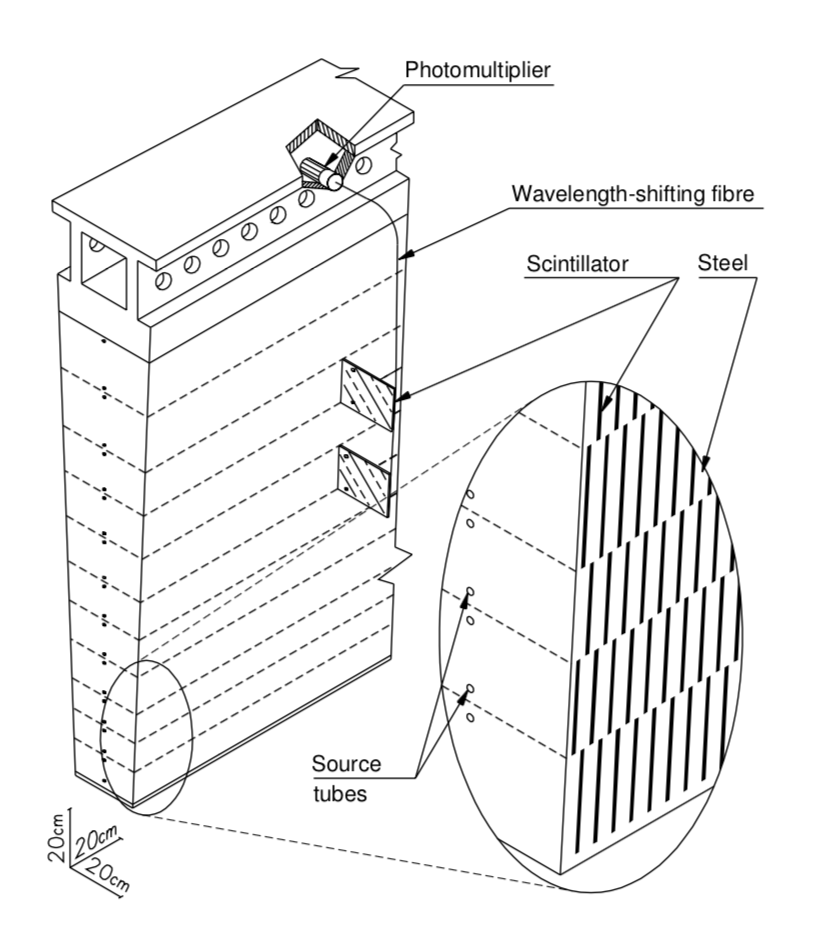
\includegraphics[width=0.6\textwidth]{tile_cal_module}
\caption{Schematic of a tile calorimeter module~\cite{atlas-detector-2008}.}
\label{fig:tile_cal_module}
\end{figure}

\begin{figure}[!ht]\centering
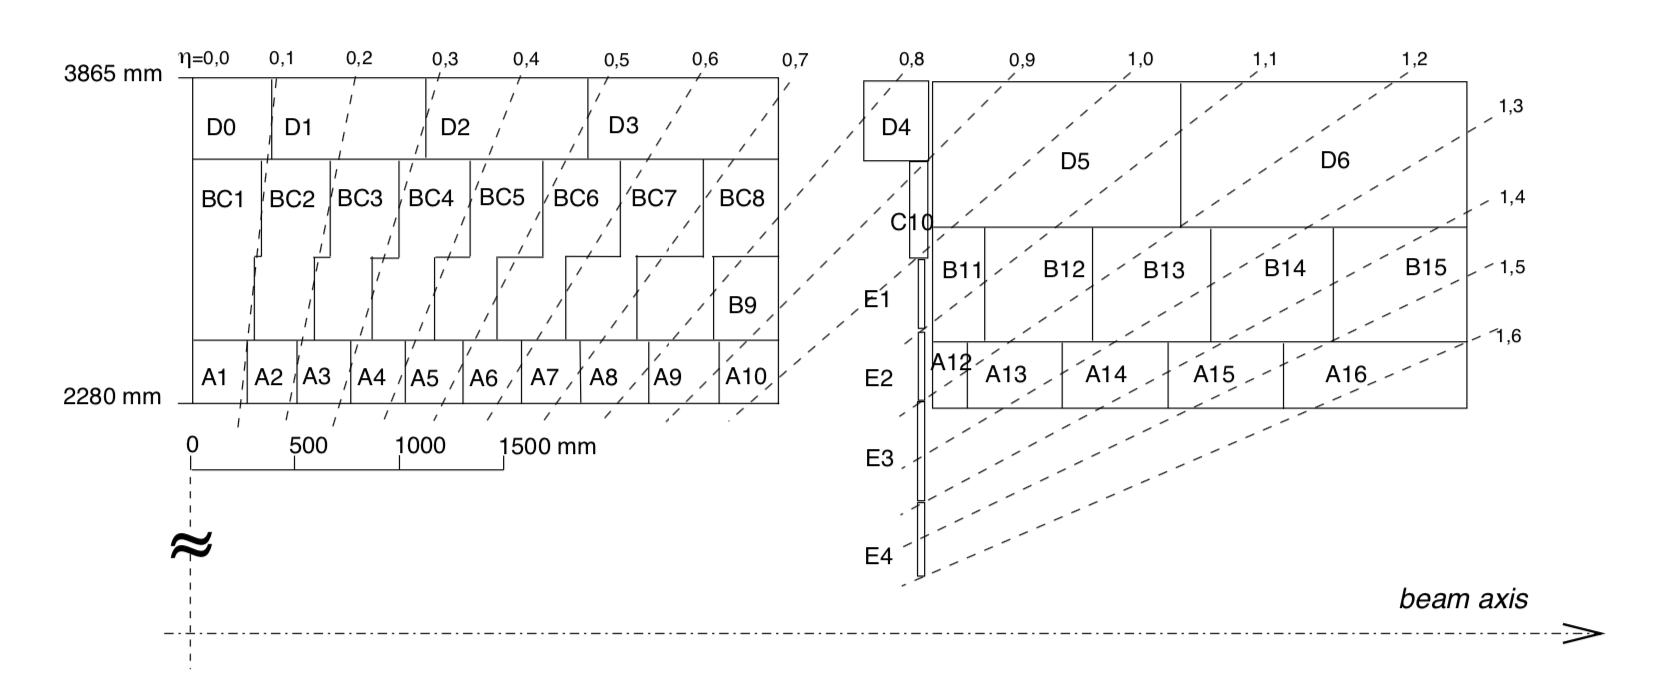
\includegraphics[width=0.9\textwidth]{tile_cal_granularity}
\caption{Schematic of the central (left) and extended (right) tile calorimeter, showing the $\eta$- and depth-dependent segmentation~\cite{atlas-detector-2008}.}
\label{fig:tile_cal_granularity}
\end{figure}

The hadronic end-cap calorimeter (HEC) consists of two cylindrical wheels on each side of the barrel, each of which has a radius of $2.03~m$.
Each of these wheels is made up of 32 modules.
The HEC wheels closest and farthest from the interaction point are called HEC1 and HEC2.
HEC1 modules have higher granularity and sample fraction than HEC2 modules.
A schematic of the HEC modules can be seen in figure~\ref{fig:hec_module}.

\begin{figure}[!ht]\centering
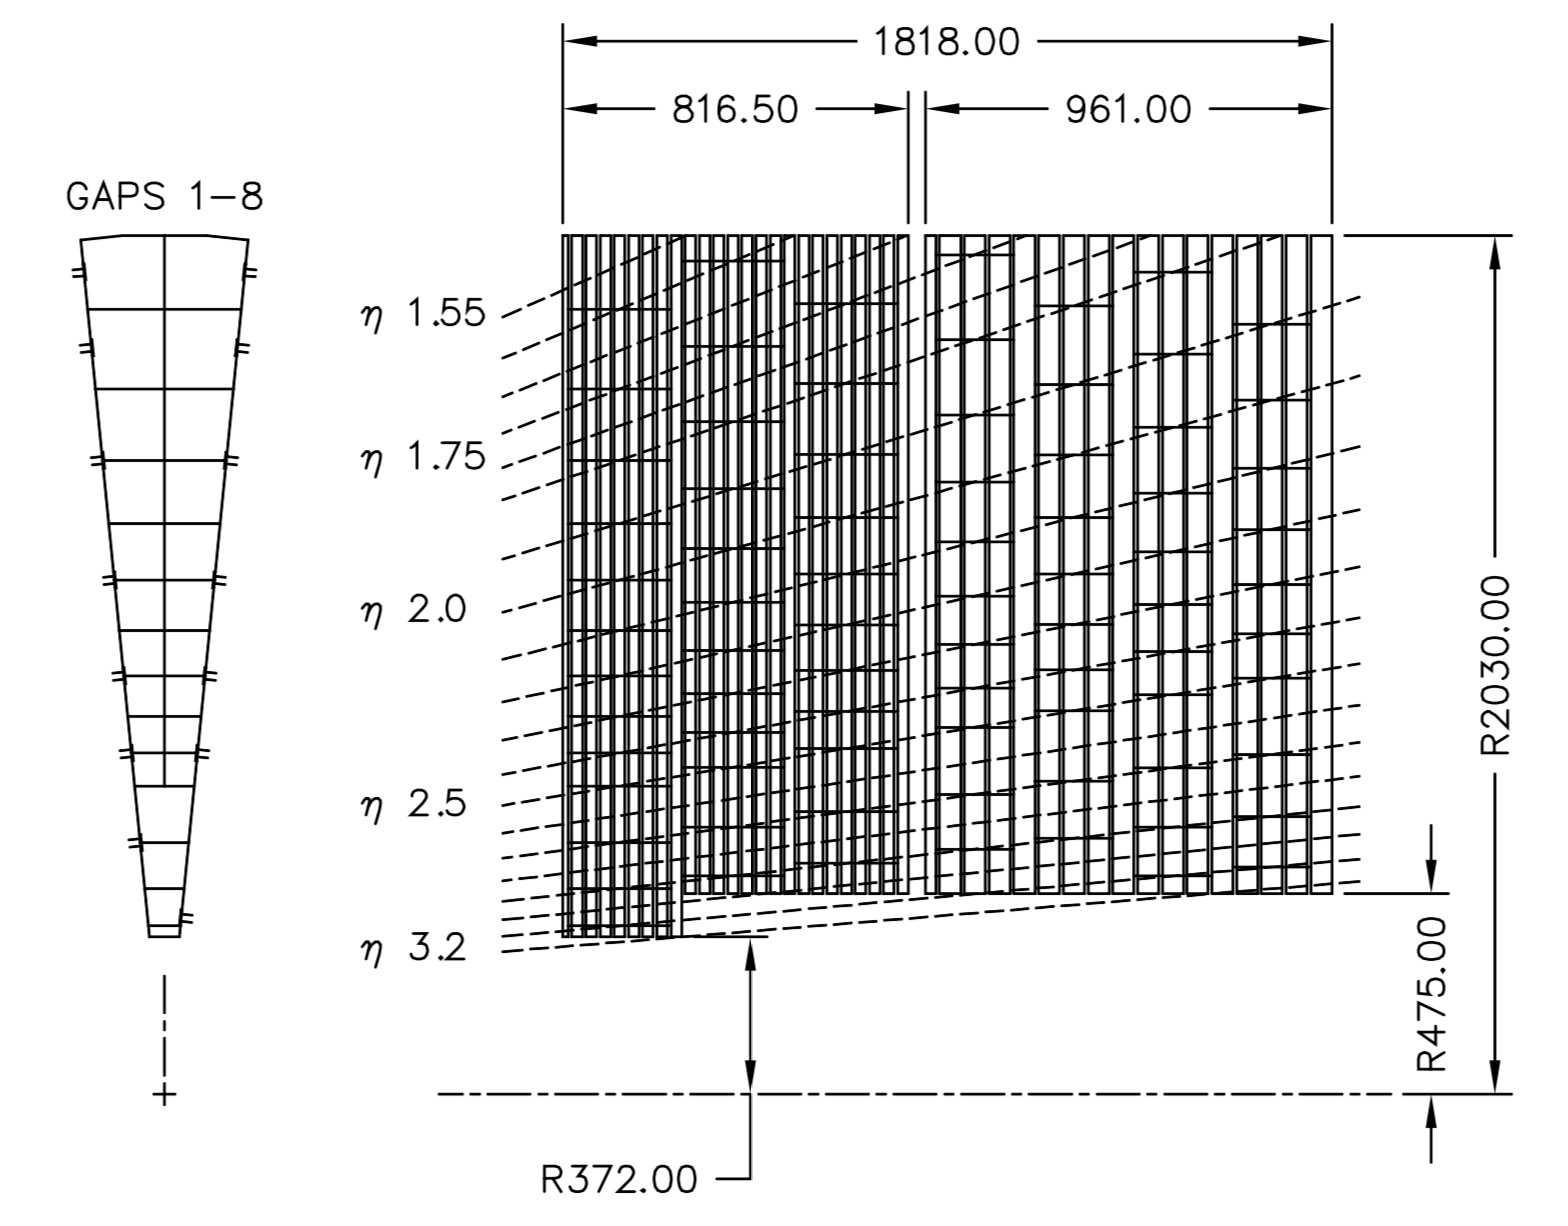
\includegraphics[width=0.6\textwidth]{hec_module}
\caption{Schematic of hadronic end-cap calorimeter module~\cite{atlas-detector-2008}.}
\label{fig:hec_module}
\end{figure}

The HECs use LAr as the sampling material and copper as the absorber material.
The copper plates are separated by gaps of $8.5~mm$, with three electrodes in between.
This creates four drift zones between each copper plate.
Typical drift time across the drift zones is $430 ns$, at a potential difference of $1800 V$~\cite{atlas-detector-2008}.
There are a total of 5632 readout cells.
In the region $|\eta| < 2.5$, the readout cell size is $\delta\phi \times \delta\eta = 0.1 \times 0.1$, and $\delta\phi \times \delta\eta = 0.2 \times 0.2$ elsewhere.

\subsubsection{Forward Calorimeters}\label{subsubsec:fcal}

Special forward calorimeters (FCal) were designed to cover the forward region, $3.1 < |\eta| < 4.9$.
This region experiences very high particle flux compared to the barrel or end-cap regions, so a different design was needed.
Each FCal consists of three modules.
The module closest to the interaction point (FCal1)is optimized for EM showers, while the middle and outer modules (FCal2 and FCal3) are optimized for hadronic showers.
All three modules are $45~cm$ deep, and use LAr as the sampling material.

FCal1 uses copper as the absorber material, while FCal2 and FCal3 use tungsten as the primary absorber.
To further reduce punch-through into the muon system, a copper shield plug is placed behind FCal3.
The location of the FCal with respect to the end-cap calorimeters can be seen in figure~\ref{fig:fcal_layout}
The FCal, hadronic end-cap, and electromagnetic end-cap calorimeters are all contained in the same end-cap cryostat.
The overlapping design of the end-cap and forward calorimeters allows for hermetic coverage with minimal energy loss out to $|\eta| < 4.9$.

\begin{figure}[!ht]\centering
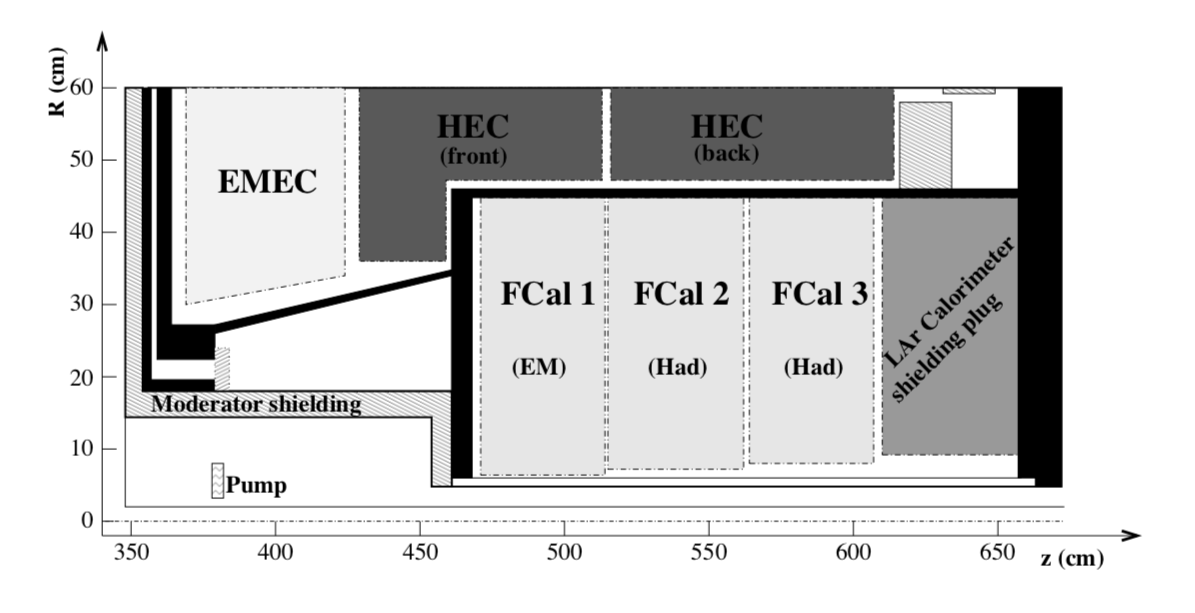
\includegraphics[width=0.9\textwidth]{fcal_layout}
\caption{Schematic showing the layout of the forward calorimeters and end-cap calorimeters~\cite{atlas-detector-2008}.}
\label{fig:fcal_layout}
\end{figure}

In order to provide accurate energy measurements of photons, jets, and $E_{Tmiss}$, it is necessary for the calorimeters to absorb as much shower energy as possible.
Any particles that don't get absorbed by the calorimeter are considered punch-through particles.
These punch-through particles reduce the accuracy of calorimeter measurements and add noise to the muon system, so they should be minimized.
For hadronic showers, the analog to a radiation length is called an interaction length, $\lambda$ .
The amount of energy absorbed by each part of the calorimeter, as measured in interaction lengths, can be seen in figure~\ref{fig:calo_material_budget}.

\begin{figure}[!ht]\centering
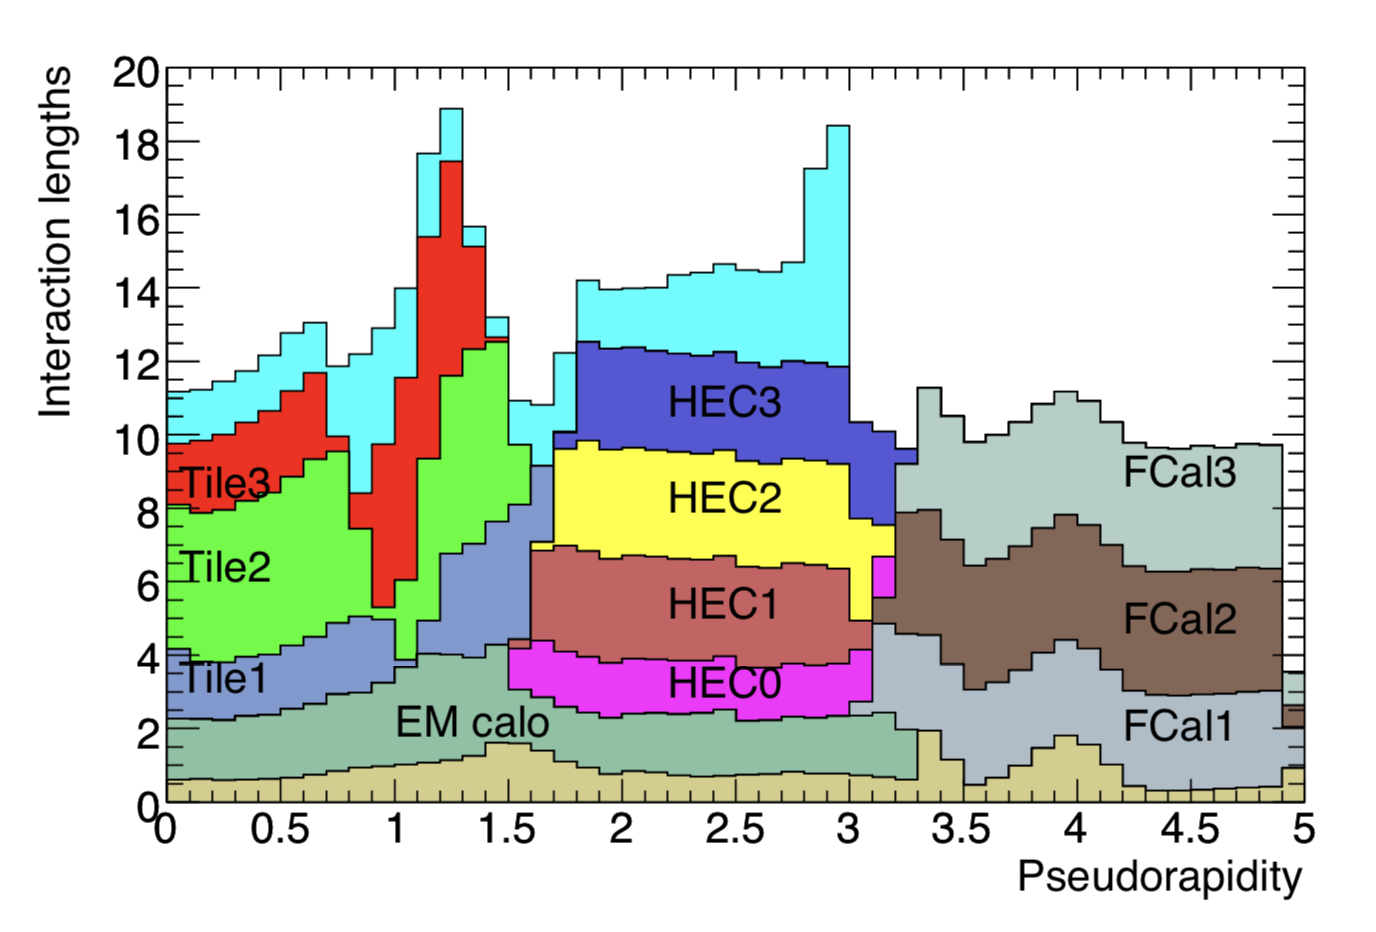
\includegraphics[width=0.9\textwidth]{calo_material_budget}
\caption{Amount of material, in units of interaction length, versus pseudorapidity, including all material before the EM calorimeter, the EM calorimeter, and the hadronic calorimeters.
The light blue indicates the amount of material in front of the muon spectrometer for $|\eta| < 3.0$~\cite{atlas-detector-2008}.}
\label{fig:calo_material_budget}
\end{figure}

\subsubsection{Energy Resolution}
The energy resolution of the LAr calorimeters is parameterised as~\cite{atlas-em-resolution}:
\begin{equation}
    \frac{\sigma(E)}{E} = \frac{a}{\sqrt{E(GeV)}}\oplus b
\end{equation}
Electron test beams ranging from $10~GeV$ to $240~GeV$ are used to measure the electron energy resolution of the LAr calorimeters.
The resulting parameters were found not to exceed $a=10\%\sqrt{GeV}$ and $b=0.7\%$ over both the EM barrel and EM end-cap calorimeters.
The hadronic end-cap calorimeter has design resolution $\frac{50\%}{\sqrt{E}}\oplus3\%$, while the forward calorimeter has design resolution $\frac{100\%}{\sqrt{E}}\oplus10\%$.
The hadronic tile calorimeter provides a jet resolution of $\sigma(E)/E = 50\%/\sqrt{E}$~\cite{atlas-detector-2008}.

\subsection{Muon spectrometer}\label{subsec:muon_spec}

The outermost ATLAS system is the muon spectrometer, used to measure the momenta of charged particles that exit the calorimeter systems.
Muons are not absorbed by the EM calorimeter because they undergo less bremsstrahlung than electrons due to their high mass.
They are also no absorbed by the hadronic calorimeter because they do not interact strongly.
As a result, muons are the most common particle to escape the calorimeter system.

The overall dimensions of the muon spectrometer, which define the demensions of ATLAS, are $44~m$ long by $22~m$ high.
The muon spectrometer consists of four subsystems.
The monitored drift tubes (MDTs) and cathode strip chambers (CSCs) are used for high-precision tracking,
while the resistive plate chambers (RDCs) and thin-gap chambers (TGCs) are used for triggering and bunch-crossing identification.
The location of each of the four muon subsystems can be seen in figure~\ref{fig:muon_spec_layout}

\begin{figure}[!ht]\centering
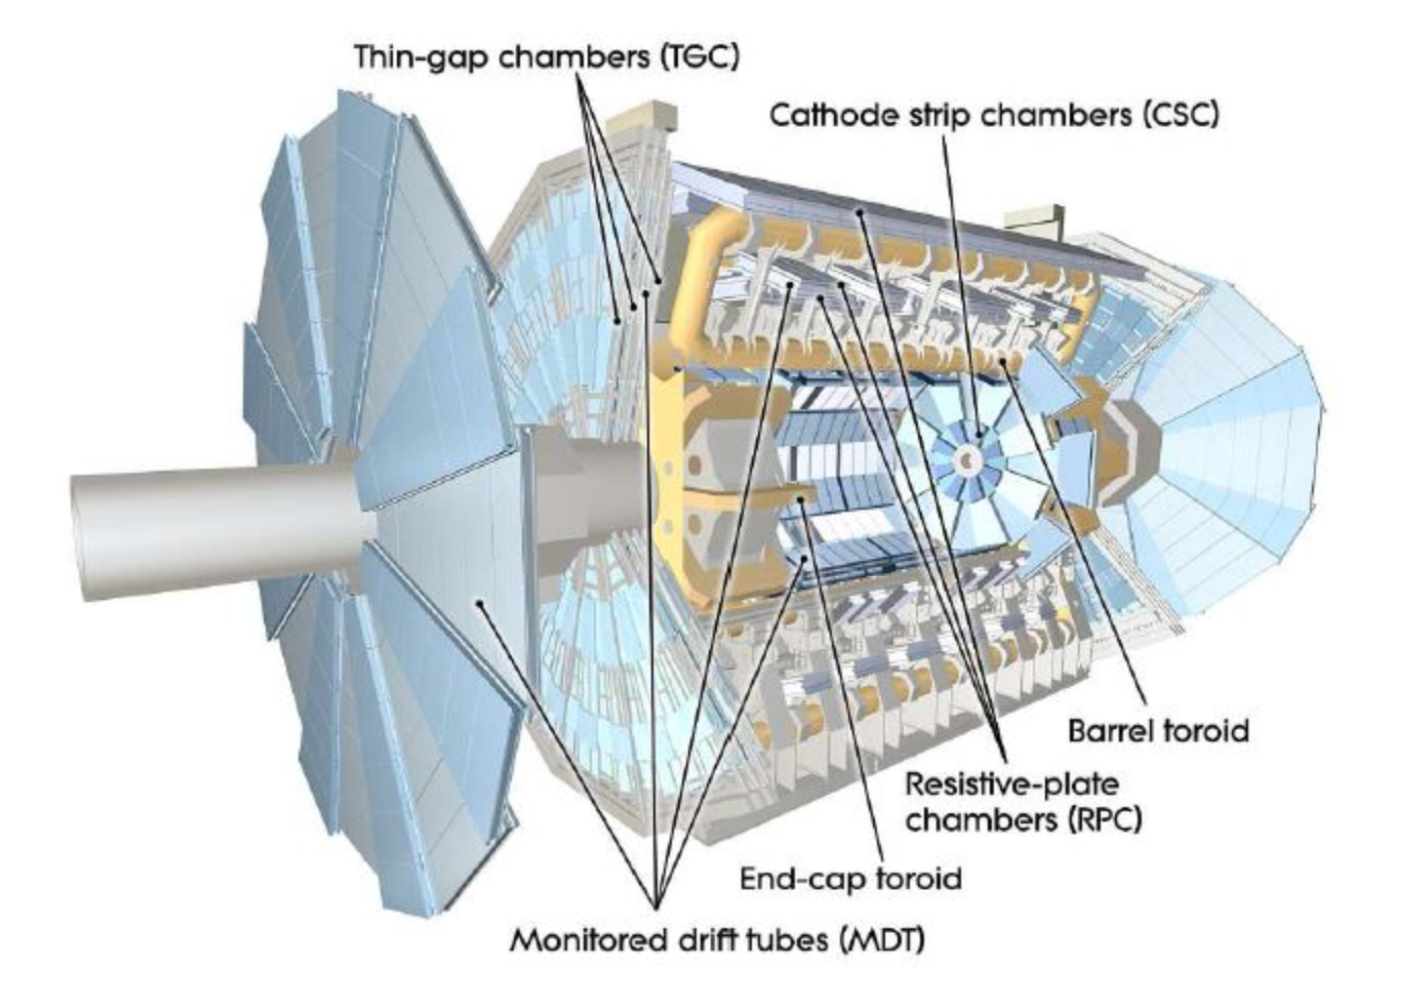
\includegraphics[width=0.6\textwidth]{muon_spec_layout}
\caption{Layout of the muon spectrometer, indicating the location of barrel and end-cap toroids, along with the four subsystems~\cite{atlas-detector-2008}.}
\label{fig:muon_spec_layout}
\end{figure}

As described in~\ref{subsec:magnet_systems}, the magnetic field in the muon system runs in a roughly circular direction around the beamline.
As a result, charged particles are bent in the $\eta$ direction in the muon spectrometer.
In the barrel region, covering $|\eta| < 1.0$ the muon system is laid out in three concentric cells, located at $5~m$, $7.5~m$, and $10~m$ from the interaction point.
Full coverage is provided in this region, except for a small gap at $|\eta| = 0$, to allow for services to the solenoid, calorimeters, and inner detector systems.
The size of the acceptance gap is $|\eta| < 0.04$ in the innermost layer, and $|\eta| < 0.08$ in the outer layers.
The end-cap consists of large wheels, located at $|z| \approx 7.4~m$, $10.8~m$, $14~m$, and $21.5~m$.
Figure~\ref{fig:muon_cross_section} shows a cross-section of the barrel region of the muon spectrometer in the $x-y$ plane, and a cross-section of the barrel and end-cap regions in the $y-z$ plane.
The small acceptance gap at $\eta = 0$ can be seen.

\begin{figure}[!ht]\centering
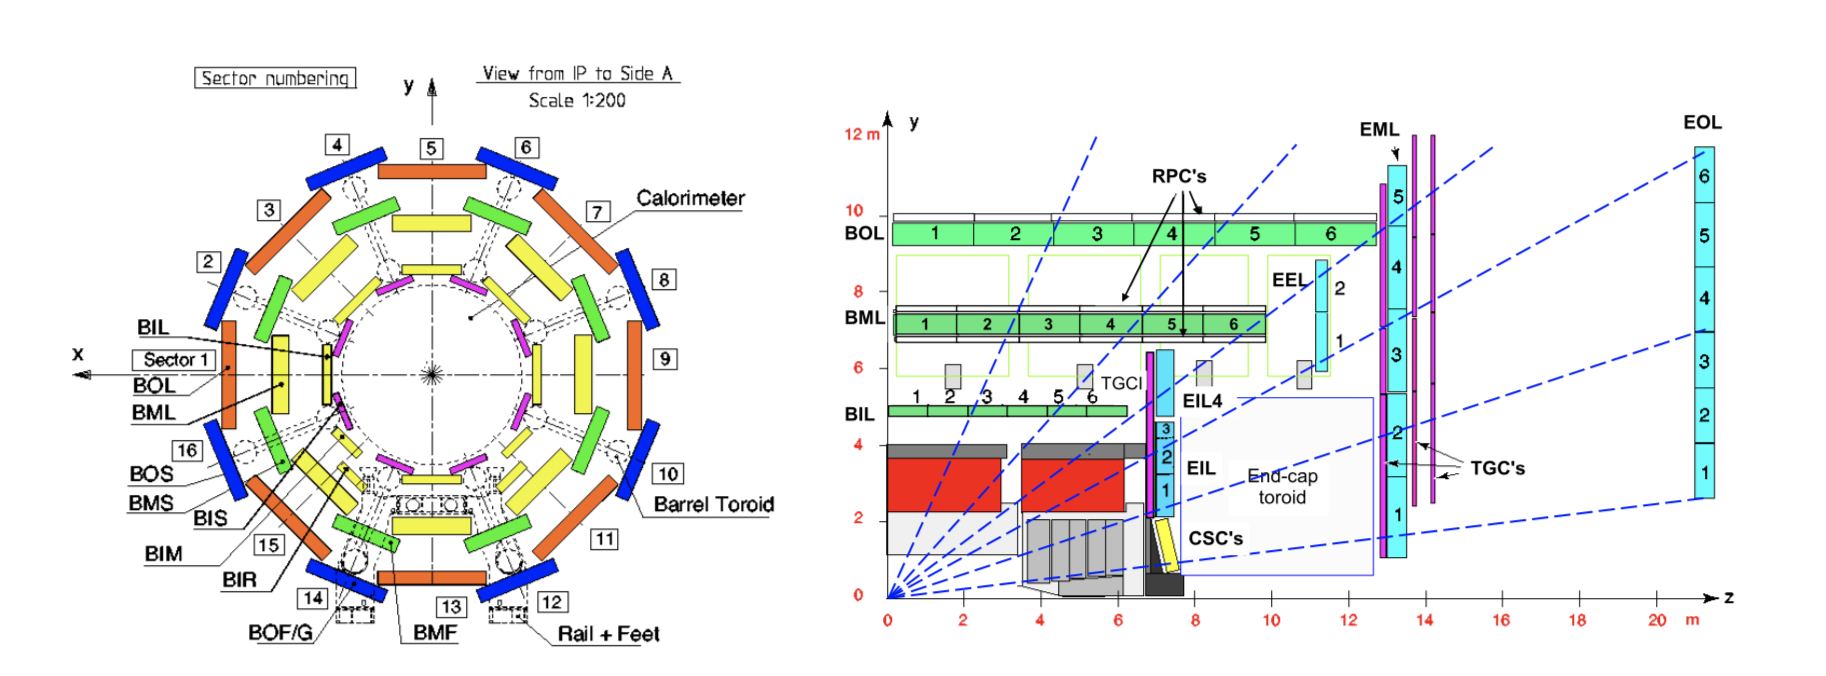
\includegraphics[width=\textwidth]{muon_cross_section}
\caption{Cross-sections in $x-y$ (left) and $y-z$ (right) of the muon spectrometer~\cite{muon-2003}.}
\label{fig:muon_cross_section}
\end{figure}

The muon spectrometer provides high-precision momentum measurements out to $|\eta| < 2.7$, and triggering on high-momentum muons out to $|\eta| < 2.4$.
The ATLAS design specification requires momentum resolution of $10\%$ for $1~TeV$ muons.
This resolution is achieved or exceeded for the range $10~GeV < p_T < 1~TeV$.
The contribution to $p_T$ resolution from various sources at different $p_T$ is shown in figure~\ref{fig:muon_resolution}.
The dominant contribution at low-$p_T$ is from energy loss fluctuations,
while at high-$p_T$ it's from wire resolution and autocalibration~\cite{muon-2003}.

\begin{figure}[!ht]\centering
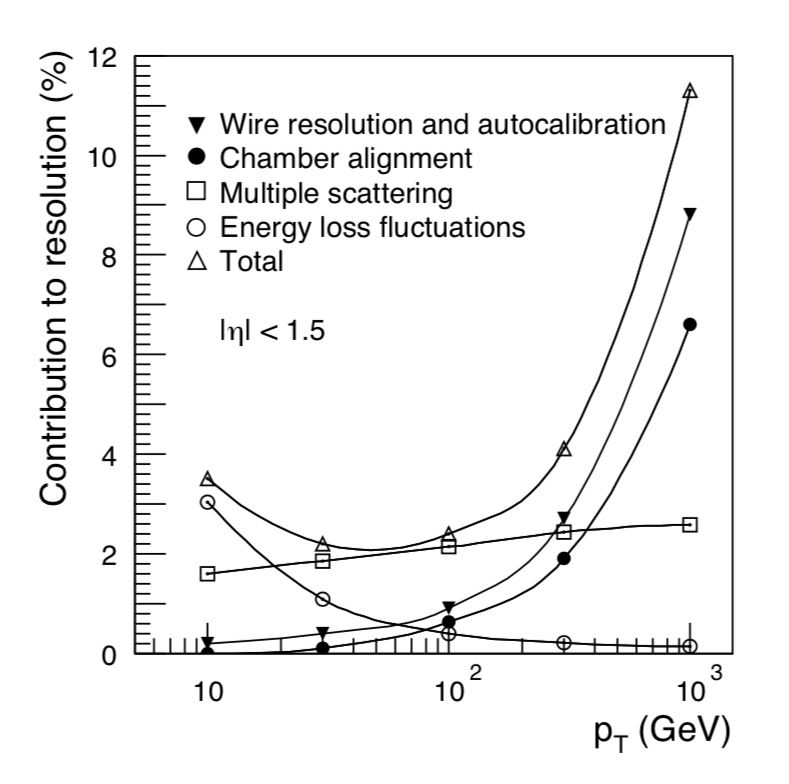
\includegraphics[width=0.6\textwidth]{muon_pt_resolution}
\caption{The contribution to muon spectrometer $p_T$ resolution from various sources over a range of $p_T$~\cite{muon-2003}.}
\label{fig:muon_resolution}
\end{figure}

Most of the precision momentum measurements in the muon spectrometer are performed by monitored drift tubes (MDTs).
The MDT subsystem covers the region $|\eta| < 2.7$, except for the innermost end-cap layer, where they cover out to $|\eta| = 2.0$.
There are a total of 1174 MDT chambers, each made up of between 3 and 8 layers of drift tubes.
The aluminum tubes are $3~cm$ in diameter and range between $0.9~m$ and $6.2~m$ in length.
They are filled with a mixture of $80~\% \mathrm{Ar}$ and  $20~\% \mathrm{CO_2}$.
The MDTs provide a resolution of $80~\mu m$ per tube, and $35~\mu m$ per chamber.
In order to provide high-precision measurements, the locations of all chambers and their support structures are constantly monitored.
Temperature and magnetic field conditions are also monitored, in order to account for thermal expansion and changes to drift time~\cite{muon-2003}.
The MDTs can be safely operated at a rate of up to $150~Hz/cm^2$.

In the innermost end-cap layer, covering the region $2.0 > |\eta| > 2.7$, the background rate is too high for safe operation of MDTs.
Instead, precision momentum measurements are performed using cathode strip chambers (CSCs), which can be safely operated at rates up to $1000~Hz/cm^2$~\cite{atlas-detector-2008}.
The CSC chambers use the same gas mixture as MDT chambers, but instead of drift tubes there are grids of anodes and cathodes, allowing for measurements of $\eta$ and $\phi$ based on the charge induced in the wires.
There are a total of 32 CSC chambers, arranged into 4 disks of 8 chambers each.
Each chamber contains 4 CSC layers, resulting in 4 independent measurements of $\eta$ and $\phi$ for each track.
Cathodes are made of $17~mm$ copper strips, and anodes are gold-plated tungsten measuring $30~mm$ in diameter.
Sense-wire pitch is $2.54~mm$, but resolution is limited by readout pitch, which is $5.08~mm$.
This results in an $\eta$ resolution of $60~\mu m$, and a $\phi$ resolution of $5~mm$~\cite{muon-2003}.
Since the magnetic fields bend muons in the $\eta$ plane, precise momentum measurements require far greater resolution in $\eta$.

Resistive plate chambers (RPCs) are used for the muon trigger in the barrel region $|\eta| < 1.05$.
In the middle station, there are two layers of RPCs, used for the low-$p_T$ threshold trigger, which has a threshold of $6-9~GeV$.
In the outer station, there is a single layer of RPCs, used for the high-$p_T$ threshold trigger, with a threshold of $9-35~GeV$.

Each RPC consists of two rectangular detectors, called units.
Standard RPCs are paired with MDTs, and have the same dimensions.
A few additional smaller RPCs are included in areas where MDTs cannot be installed due to lack of space.
Each RPC provides two measurements of $\eta$ and $\phi$ for a charged particle passing through it.
A charged particle passing through all three layers therefore generates 6 $\eta-\phi$ measurements.
To reduce fake tracks, 3 out of 4 of the middle-station detectors and at least one outer layer station must register hits.

An RPC detector consists of two plastic insulating plates, separated by $2~mm$, with a gas occupying the internal space, and a voltage difference of $9.8~kV$ across the plates.
Charged particles passing through the plates generate an avalanche of charge which can then be measured by metallic strips connected to the plates.
The insulator plates are made of phenolic-melaminic plastic laminate, and the gas is a mixture of $\mathrm{C_2 H_2 F4}$, $\mathrm{Iso-C_4 H_{10}}$, and $\mathrm{SF_6}$ in the proportions $94.7\%$, $5\%$, $0.3\%$~\cite{atlas-detector-2008}.
The RPCs provide a time resolution of $2~ns$.

In the forward region, $1.05 < |\eta| < 2.4$, muon triggering is provided by thin-gap chambers (TGCs).
TGCs also provide a $\phi$ measurement to complement the $\eta$ measurement provided by the MDTs.
In the MDT end-cap middle layer, there are seven layers of TGCs, and in the inner layer, there are 2 layers of TGCs.
Each TGC layer consists of two concentric rings.

Like the CSCs, the TGCs are multi-wire proportional chambers (MWPCs).
To reduce drift time so that an acceptable time resolution can be achieved, the drift distance must be kept small, and the electric field kept high.
The wire-to-cathode distance is $1.4~mm$ in the TGCs, even closer than the wire-to-wire distance of $1.8~mm$, and the voltage is kept at $2.9~kV$.
A highly quenching gas mixture of $55\% \mathrm{CO_2}$ and $45\% \mathrm{n-C_5 H_{12}}$ is used in the TGCs~\cite{atlas-detector-2008}.
The resulting time resolution provided by the TGCs is $4~ns$~\cite{muon-2003}.

\subsection{Trigger}\label{subsec:trigger}

Because of the very high event rate at the LHC, and the large amount of data collected per event, it is impossible to record every single event.
There are 40 million bunch crossings per second, and each collision can generate $1.6~MB$ of raw data.
The ATLAS trigger system is designed to make very fast decisions about which events to record and which to ignore, in order to reduce the event rate to approximately $1~kHz$.
The challenge of trigger design is to balance processing time against decision accuracy, to make sure that events that could be useful for physics analysis are not lost.
The selection criteria used by each level of the trigger are known as the trigger menu.
A large number of possible trigger selection criteria are designed, in order to serve the broad range of physics analyses performed at ATLAS .

The ATLAS trigger system consists of a hardware based level 1 (L1) trigger and a software-based high-level trigger (HLT).
The L1 trigger reduces the event rate from the original $40~MHz$ to approximately $100~kHz$.
The HLT further reduces the event rate to approximately $1~kHz$, which is the maximum rate of data transfer from the detector.
The flowchart of data through the trigger system can be seen in figure~\ref{fig:trigger_flowchart}

\begin{figure}[!ht]\centering
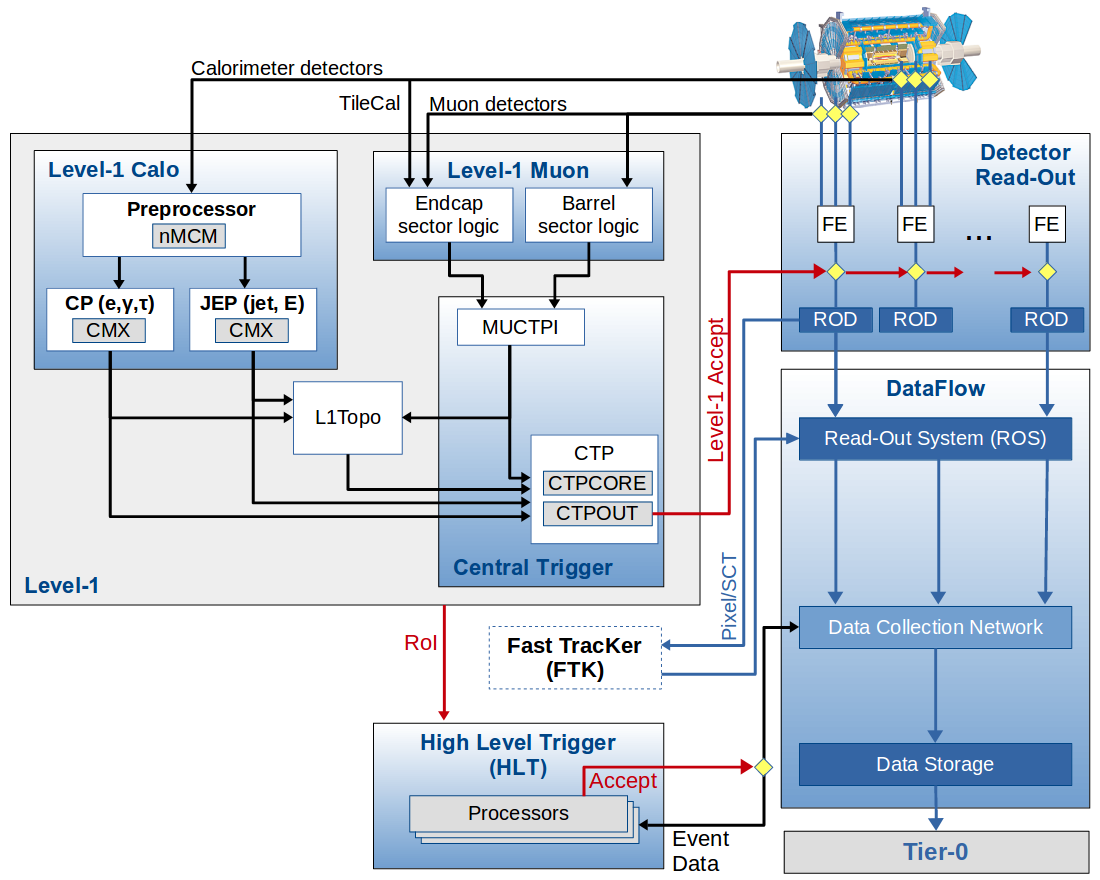
\includegraphics[width=0.9\textwidth]{trigger_flowchart}
\caption{Flowchart outlining the level 1 and high-level trigger design and data acquisition system~\cite{atlas-trigger}.}
\label{fig:trigger_flowchart}
\end{figure}

For every event, the L1 trigger system reads reduced-granularity measurements from both the hadronic and electromagnetic calorimeters.
Special calorimeter cells, called trigger towers, in each calorimeter were designed for this purpose.
The trigger towers have a granularity of $\delta \eta \times \delta \phi = 0.1 \times 0.1$.
The location of the trigger towers at the back of the electromagnetic calorimeter can be seen in figure~\ref{fig:em_calo}.
The L1 trigger also reads data from the RPCs and TGCs of the muon spectrometer system, as discussed in~\ref{subsec:muon_spec}.
The calorimeter data will be used for photon, electron, tau, jet, and $E_{Tmiss}$ triggers, and the muon data will only be used for muon triggers.
Data from these two sources are fed into the central trigger processor (CTP), which makes the decision about whether or not accept each event at level 1.

If an event is accepted at L1, full detector raw data for that event is read out and temporarily stored until the HLT decision is made, and some amount of reconstruction is done at this time.
Later, if an event is accepted by the HLT, the full tracking reconstruction algorithm will be applied.
The L1 system then sends region-of-interest information to the HLT .
Regions of interest are the subsections of the detector that the L1 trigger has identified as possibly containing interesting physics objects.
The full detector information and L1 region-of-interest data are combined by the HLT, which then makes the final decision on whether or not to keep an event.
Only when an event passes both the L1 and HLT decision criteria will its be permanently stored.
The L1 trigger system decision time is just $2.5~\mu s$, while the HLT makes decisions on the order of seconds.

\chapter{Jets} \label{ch:jets}

A jet is a collimated spray of stable particles measurable in the detector,
which arises from the production of a quark or gluon in the scattering process.
Due to QCD confinement, the quarks and gluons themselves can never be observed,
so jets serve as an observable proxy for these more fundamental particles.
However, there is not a simple one-to-one correspondence between each jet measured in an event and a quark or gluon in the hard scattering process.
Due to the complex nature of proton-proton collisions, as well as the fundamental probabilistic nature of quantum mechanics, the partonic source for a given jet can never be specified exactly.
Likewise, when performing theoretical calculations, the number and property of jets that arise from a given parton produced in the hard scattering can only be specified probabilistically.
Section~\ref{sec:jet_collisions} will explain the many different parts of a proton-proton collision that contribute to jet production.

Furthermore, the number and properties of jets measured in a single event will depend on the choice of jet reconstruction algorithm.
In order for experimentalists to test the predictions of theory, it's important for standard jet definitions to be decided upon.
While there is no one theoretically correct choice of jet definition, there are certain properties of jet algorithms that make them more or less desirable.
The different kinds of jet algorithms and their properties will be discussed in section~\ref{sec:jet_clustering}.
Section~\ref{sec:jet_mass} will explain the origin of jet mass and how it can be accurately reconstructed.
And section~\ref{sec:jet_reconstruction} will explain the process of jet reconstruction and calibration in ATLAS .

\section{The proton-proton collision environment}\label{sec:jet_collisions}

As discussed in~\ref{subsec:qcd_pdfs}, the goal of proton-proton collision experiments is to understand the interactions
between fundamental particles, but due to QCD confinement it is impossible to simply collide the individual partons of interest.
Instead, complicated bound states of quarks and gluons are collided,
with the goal of measuring the processes that occur when constituent partons collide with each other.
As a result, proton-proton collision events create a very messy environment from which the hard-scatter process
has to be deduced.

QCD confinement also has the consequence that the final state quarks and gluons created in LHC collisions
can never be directly detected.
Instead, collimated sprays of hadrons, called jets, must be measured in order to attempt to reconstruct the
hard scattering process that gave rise to them.

Figure~\ref{fig:jet_tth_diagram} illustrates a representative proton-proton collision event.
Even though this is not a dijet or multijet production event, it is useful for understanding all the parts of a proton-proton collision that must be considered when calculating the predicted rates of multijet production.

\begin{figure}[!ht]
    \centering
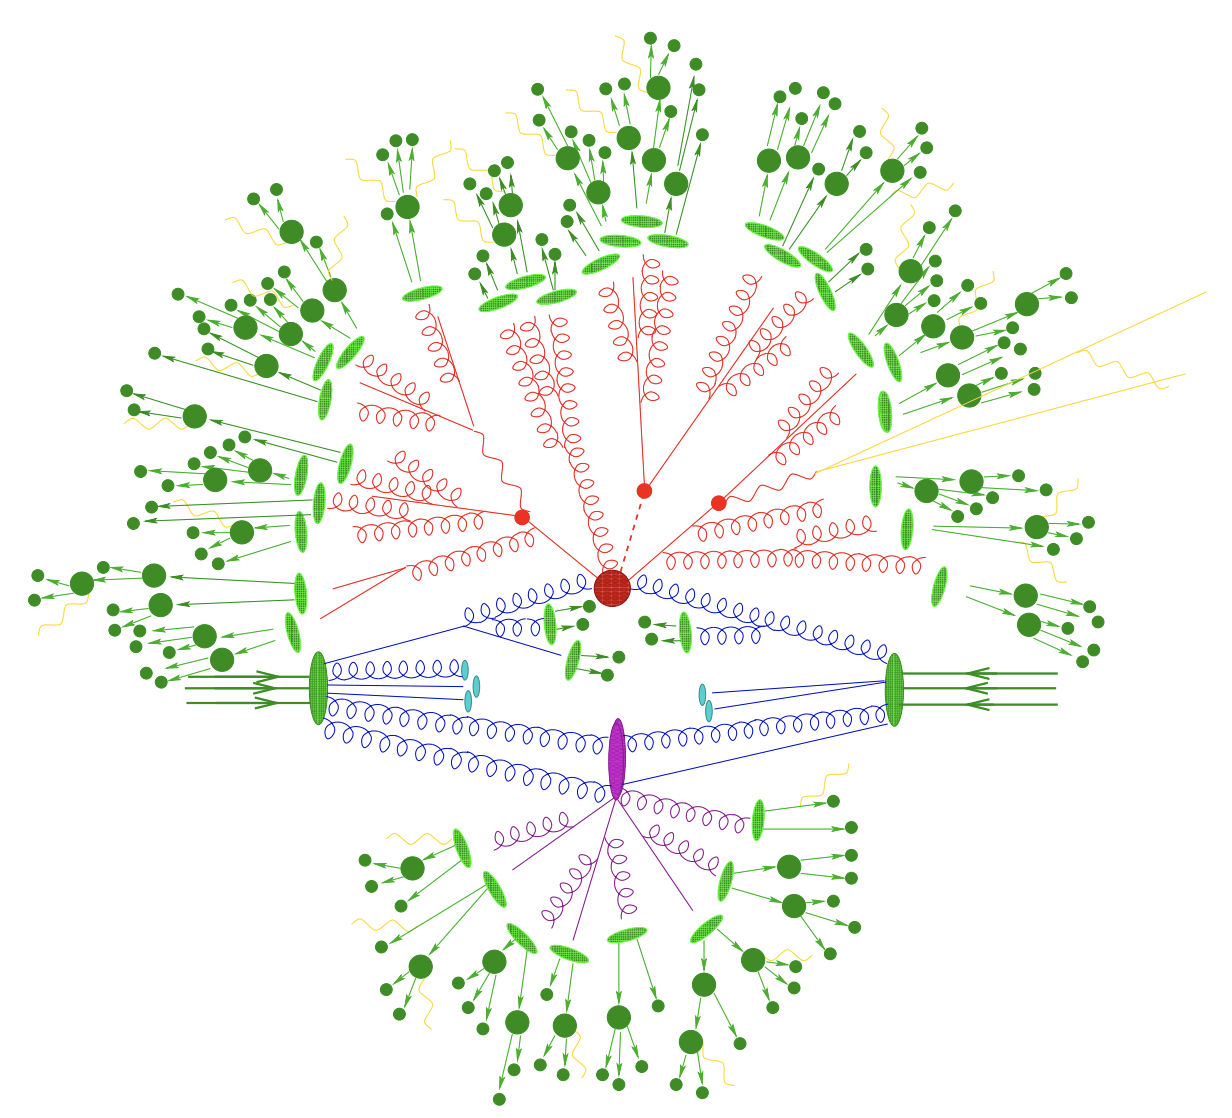
\includegraphics[width=0.8\linewidth]{jet_tth_diagram}
\caption{Diagram of a proton-proton collision event.
Illustrated are the initial state radiation, underlying event, hard-scatter process, final state parton shower,
fragmentation, hadron decays, and final state QED radiation~\cite{sherpa-2004}.}
\label{fig:jet_tth_diagram}
\end{figure}
The incoming protons are illustrated by green blob with three incoming arrows to represent the constituent valence quarks.
The initial state parton shower, governed by QCD, is shown in blue.
The hard scatter process is represented by the large red circle.
Quarks and gluons from the incoming proton that do not participate in the hard scatter process can nonetheless interact with each other, creating a so-called underlying event, shown in purple.
All of the strongly-interacting final state quarks and gluons undergo final state parton showering, also in red.
Once the final state parton shower particles reach a low enough energy, they hadronize, in a non-perturbative process represented by the light green blobs.
The resulting hadrons then decay through various decay chains, shown in dark green.
Photon radiation, governed by QED, can occur at any of these stages, and is shown in yellow.

Accurate modelling of multijet events is challenging for several reasons.
The first challenge comes from merging the matrix-element differential cross section with the parton shower simulation
An event with $n$ jets in the final state can arise from a hard scattering event with $n$ partons in the final state, or from an event with $n-1$ partons in the final state, where the additional jet arises during the parton shower.
The contributions from these two paths cannot be exactly factorized, but different merging schemes have been developed to combine them in a way that avoids double counting and yields accurate estimates of jet kinematic observables~\cite{jet-merging}.
Uncertainties necessarily arise from the choice of merging scheme and scale parameters.
There are additional uncertainties from higher-order diagrams, which can be evaluated by observing the change in cross section as the QCD scale is varied.
High jet multiplicity events require diagrams with more factors of $\alpha_{s}$, so the uncertainty from higher-order diagrams grows with jet multiplicity.
Additional contributions to uncertainty come from the choice of PDF and from the underlying event.
Figure~\ref{fig:jet_multijet_uncertainties} shows the sizable discrepancy in third-jet $p_{T}$ and jet multiplicity distributions across several event generators.
Because of the challenges in using Monte Carlo to estimate QCD multijet cross sections, the analysis presented in this thesis will use a fully data-driven background estimation method.
\begin{figure}[!ht]
    \centering
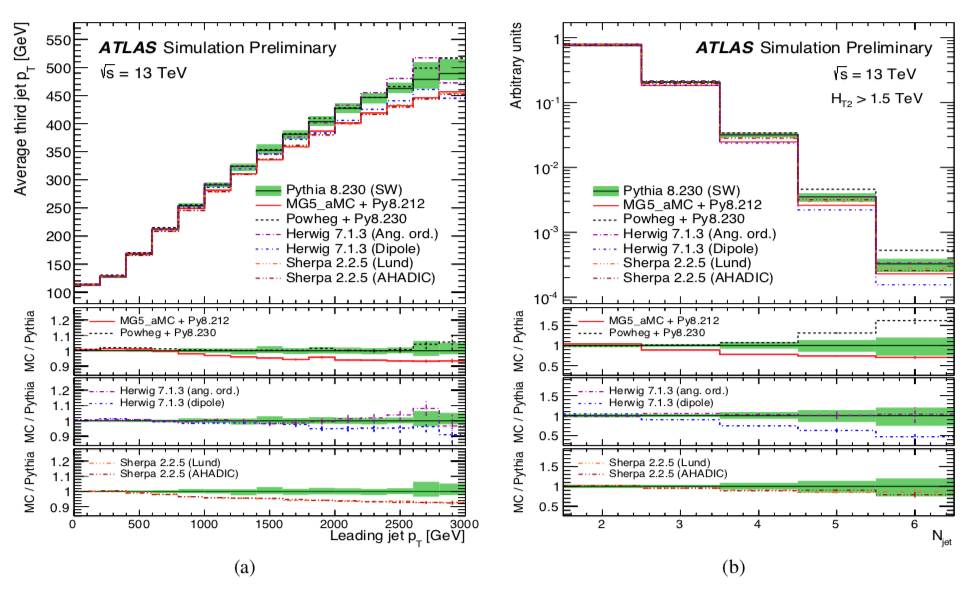
\includegraphics[width=0.9\linewidth]{jet_multijet_simulation}
\caption{Distribution of third-leading jet $p_{T}$ vs. leading jet $p_{T}$ (left) and jet multiplicity (right) for events simulated with several different event generators and parton shower methods.
The bottom pane of each plot shows the ratio with respect to the Pythia 8 result.
~\cite{jet-multijet-simulation}.}
\label{fig:jet_multijet_uncertainties}
\end{figure}

\section{Clustering algorithms}\label{sec:jet_clustering}

In order to measure jets in an event, a decision has to be made on the type of jet reconstruction algorithm to use.
The observable result of a collision event can consist of many clusters of stable particles or calorimeter hits.
Exactly which particles to cluster together is highly non-trivial, and developing the algorithms to make these decisions is an active area of research in particle physics.
The 1990 Snowmass accord defined a set of criteria which should be met by any jet algorithm.
The criteria for a developing a jet reconstruction algorithm are~\cite{jet-jetography,jet-snowmass}:

\begin{enumerate}
    \item Simple to implement in an experimental analysis
    \item Simple to implement in the theoretical calculation
    \item Defined at any order in perturbation theory
    \item Yields finite cross sections at any order of perturbation theory
    \item Yields a cross section that is relatively insensitive to hadronization
\end{enumerate}

Jet reconstruction algorithms that meet all of these criteria allow experimentalists to test theoretical predictions, because both the theoretical calculations and experimental analysis can use the same jet definition.
Jet algorithms are defined as acting on abstract "objects".
The fifth Snowmass criterion ensures that in theoretical calculations, jet algorithms can be applied at either the parton-level or hadron level.
In either case, the object which the algorithm acts on will be a particle.
Jet algorithms can also be applied by experimentalists to reconstruct jets from either simulated or real calorimeter hits.
In this case, the object which the algorithm acts on is a cluster of calorimeter hits.

Historically, there have been two major types of jet algorithms used in particle physics experiments: cone-based algorithms and sequential recombination algorithms.
Cone-based algorithms aim to cluster jets in $\eta-\phi$ space.
They are fast and easy to implement, and produce jets with regular boundaries in $\eta-\phi$ space, but have many theoretical and practical downsides compared to sequential recombination algorithms.
They typically use the highest-transverse-momentum (hardest) object in the event as a seed for a jet cone, then define a cone around that seed as the leading jet, before moving on to the next-hardest object.
Cone-based algorithms have the advantage of producing regularly-shaped jet boundaries, which can simplify theoretical calculations and make experimental calibration easier~\cite{jet-cone-algo}.
However, cone-based algorithms typically lack collinear safety\footnote{The exception to this is the SISCone algorithm~\cite{jet-siscone-algorithm}, a cone-based algorithm which is both IR and collinear safe.}, which is a property that must be satisfied to meet the Snowmass criteria.

\subsection{IRC safety}\label{subsec:jet_irc_safety}

Jet algorithms should ideally possess infrared and collinear (IRC) safety.
This means that their results should not change due to soft gluon emissions or near-collinear emissions during either the parton shower or hadronization process.
IRC safety is important because soft and collinear emissions are extremely common in QCD, and create divergences in perturbative calculations if the algorithm is IRC-unsafe~\cite{jet-jetography}.

\subsubsection{Collinear safety}

A collinear-safe algorithm is insensitive to near-collinear emissions that occur during parton showering or hadron decays.
Most cone-based algorithms are not collinear-safe because they seed jets with the hardest object in the event, which is very likely to change if there is a near-collinear emission.

In figure~\ref{fig:jet_collinear_safety}, for the collinear-unsafe cone-based algorithm, the hardest object in the event changes depending on whether the radiated gluon is reabsorbed or emitted nearly collinear to the original quark.
Thus, the resulting seed will change, yielding different jet results.
The loop diagram and collinear emission diagram both lead to divergences in the theoretical cross-section.
In a collinear-safe algorithm, the two divergences would cancel out because both amplitudes must be added to calculate the rate of the single jet being produced.
But in a collinear-unsafe algorithm, the two divergences do not cancel out, so perturbation cross-sections are not finite.

\begin{figure}[!ht]
    \centering
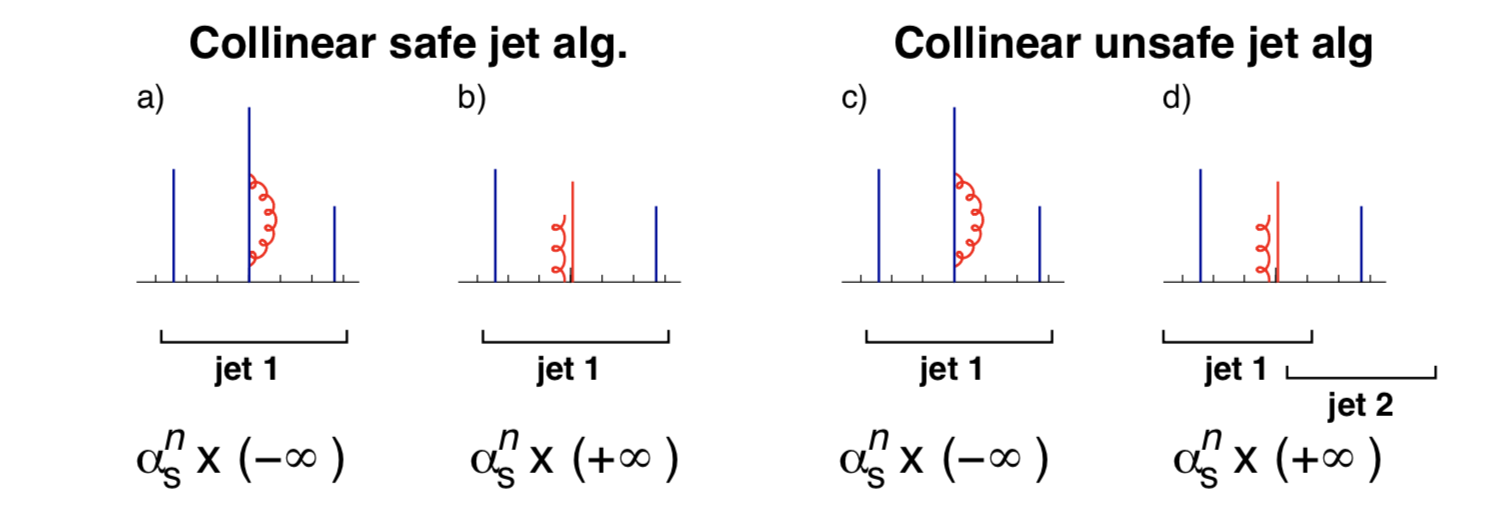
\includegraphics[width=0.9\linewidth]{jet_collinear_safety}
\caption{Illustration comparing collinear-safe (left) and collinear-unsafe (right) jet clustering algorithms.
The emission of a near-collinear gluon changes the number of jets in the event, and results in diverges in theoretical calculations.
The x-axis represents rapidity, and y-axis represents transverse momentum~\cite{jet-jetography}.}
\label{fig:jet_collinear_safety}
\end{figure}

\subsubsection{Infrared safety}

A related concept is that of infrared safety.
Jet algorithms should insensitive to soft gluon emissions.
These emissions are extremely common during parton showering, and since they occur in the non-perturbative regime of QCD,
very hard to accurately predict.

Figure~\ref{fig:jet_ir_safety} illustrates the result of an infrared-unsafe algorithm.
A W boson decays to a quark-antiquark pair, which should result in two hard jets.
Diagrams (b) and (c) each lead to IR divergences, which would cancel if the algorithm is infrared-safe.
But for an infrared-unsafe algorithm, diagram (c) leads to a different number of jets from diagram (b), so the divergences do not cancel~\cite{jet-jetography}.

\begin{figure}[!ht]
    \centering
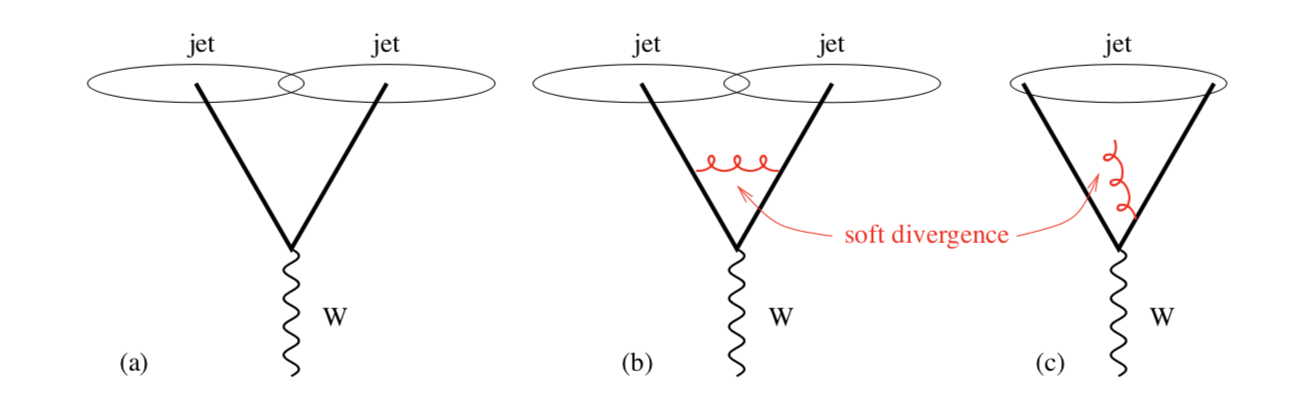
\includegraphics[width=0.9\linewidth]{jet_ir_safety}
\caption{Illustration of infrared unsafety.
In an event with a W boson decaying to two hard partons, the emission of a soft gluon can change the result of an infrared-unsafe algorithm~\cite{jet-jetography}.}
\label{fig:jet_ir_safety}
\end{figure}

\subsection{Sequential recombination algorithms}\label{subsec:jet_seq_recombination}

Sequential recombination algorithms are the most commonly used jet algorithms in ATLAS today.
Instead of clustering in $\eta-\phi$ space, they cluster in transverse momentum space.
The resulting jets have irregular boundaries, which adapt to soft radiation.
Sequential recombination algorithms are generally slower to run,
but have become more popular since the invention of the FastJet algorithm~\cite{jet-fastjet}.
The sequential recombination algorithms discussed here are IRC safe.

All sequential recombination algorithms start by defining the distance measures:

\begin{align}\label{eq:jet_distance}
    d_{ij} = min\left(k_{Ti}^{2p}, k_{Tj}^{2p}\right)\frac{\Delta_{ij}}{R^2} \\
    d_{iB} = k_{Ti}^{2p}
\end{align}
where the indices $i$ and $j$ are used for two objects under consideration, $d_{ij}$ is the distance between those two objects, $k_T$ is the transverse momentum, $\Delta_{ij}^2 \equiv (\eta_i-\eta_j)^2 + (\phi_i-\phi_j)^2$ is the distance-squared in $\eta-\phi$ space, and $p$ and $R$ are two parameters that control the behavior of the algorithm.
The object-beam distance, $d_{iB}$ is also used by the algorithms, and is defined for each object individually rather than for pairs of objects.
The choice of $R^2$ roughly controls the area of the resulting jets.
It is often referred to as a radius parameter, but the jets that result from these algorithms have irregular shapes, so this term is used loosely.
The choice of $p$ determines the class of sequential recombination algorithms, each of which has different properties.
The steps are then all the same for all sequential recombination algorithms:
\begin{enumerate}
    \item Calculate $d_{ij}$ over all pairs of objects, and $d_{iB}$ for each object individually
    \item If the minimum of the set $\{d_{ij}, d_{iB}\}$ is one of the $d_{ij}$'s:
        \subitem Sum the four vectors of objects $i$ and $j$
        \subitem Add the resultant four-vector to the list of objects, and remove the four vectors for objects $i$ and $j$
        \subitem Go to Step 1
    \item Else if the minimum of the set $\{d_{ij}, d_{iB}\}$ is one of the $d_{iB}$'s:
        \subitem Call the object $i$ a jet
        \subitem Remove the object $i$ from the list of objects
        \subitem Go to Step 1
\end{enumerate}
An inclusive clustering algorithm stops when all objects have been clustered into a jet, while an exclusive algorithm stops when a pre-defined number of jets have been clustered~\cite{jet-algo-review}.

The Cambridge-Aachen (C/A) algorithm has $p=0$, and so does not directly use the transverse momentum of the jets.
Instead the distance measures are purely in terms of pseudorapidity and azimuthal angle, so objects are clustered based on how close together they are in this radial distance measure.
The boundaries of resulting jets are sensitive to random fluctuations of soft objects, such as those from pileup and the underlying event.

The $k_T$ algorithm has $p=1$, and so starts by clustering objects which are both spatially close together and have low momentum.
Like with the C/A algorithm, the resulting jets are sensitive to random fluctuations in soft objects from pileup and the underlying event.

In the anti-$k_T$ algorithm, the objects which are closest together and hardest are clustered together first.
The resulting jet shapes are insensitive to the details of the soft radiation.
As a result, the impact of pileup and the underlying event on jet momentum resolution is smallest for the anti-$k_T$ algorithm~\cite{jet-antikt-algo}.

A comparison of the different jet clustering algorithms can be seen in figure~\ref{fig:jet_algo_compare}.
The same parton-level simulated event data was input into four different jet clustering algorithms.
Random soft particles were also added to the parton-level event data.
The resulting jets are plotted in $y-\phi$ space, with colors labelling the different jets, and the height of each bar indicating the transverse momentum in that region.
For the $k_T$ and $C/A$ algorithms, the jet boundaries are highly irregular, and depend strongly on the details of the random soft particles~\cite{jet-antikt-algo}.

ATLAS uses the ant-$k_T$ algorithm for its jet reconstruction because of its lack of sensitivity to pileup and underlying event, as well as its regular jet boundaries.
The standard choice of radius parameter used by ATLAS is $R=0.4$, and a radius parameter of $R=1.0$ is used for large-$R$ jets, as discussed in the next section.
This analysis uses both small-$R$ and large-$R$ jets, which requires running the jet clustering algorithm twice for each event, starting from the topo-clusters each time.

\begin{figure}[!ht]
    \centering
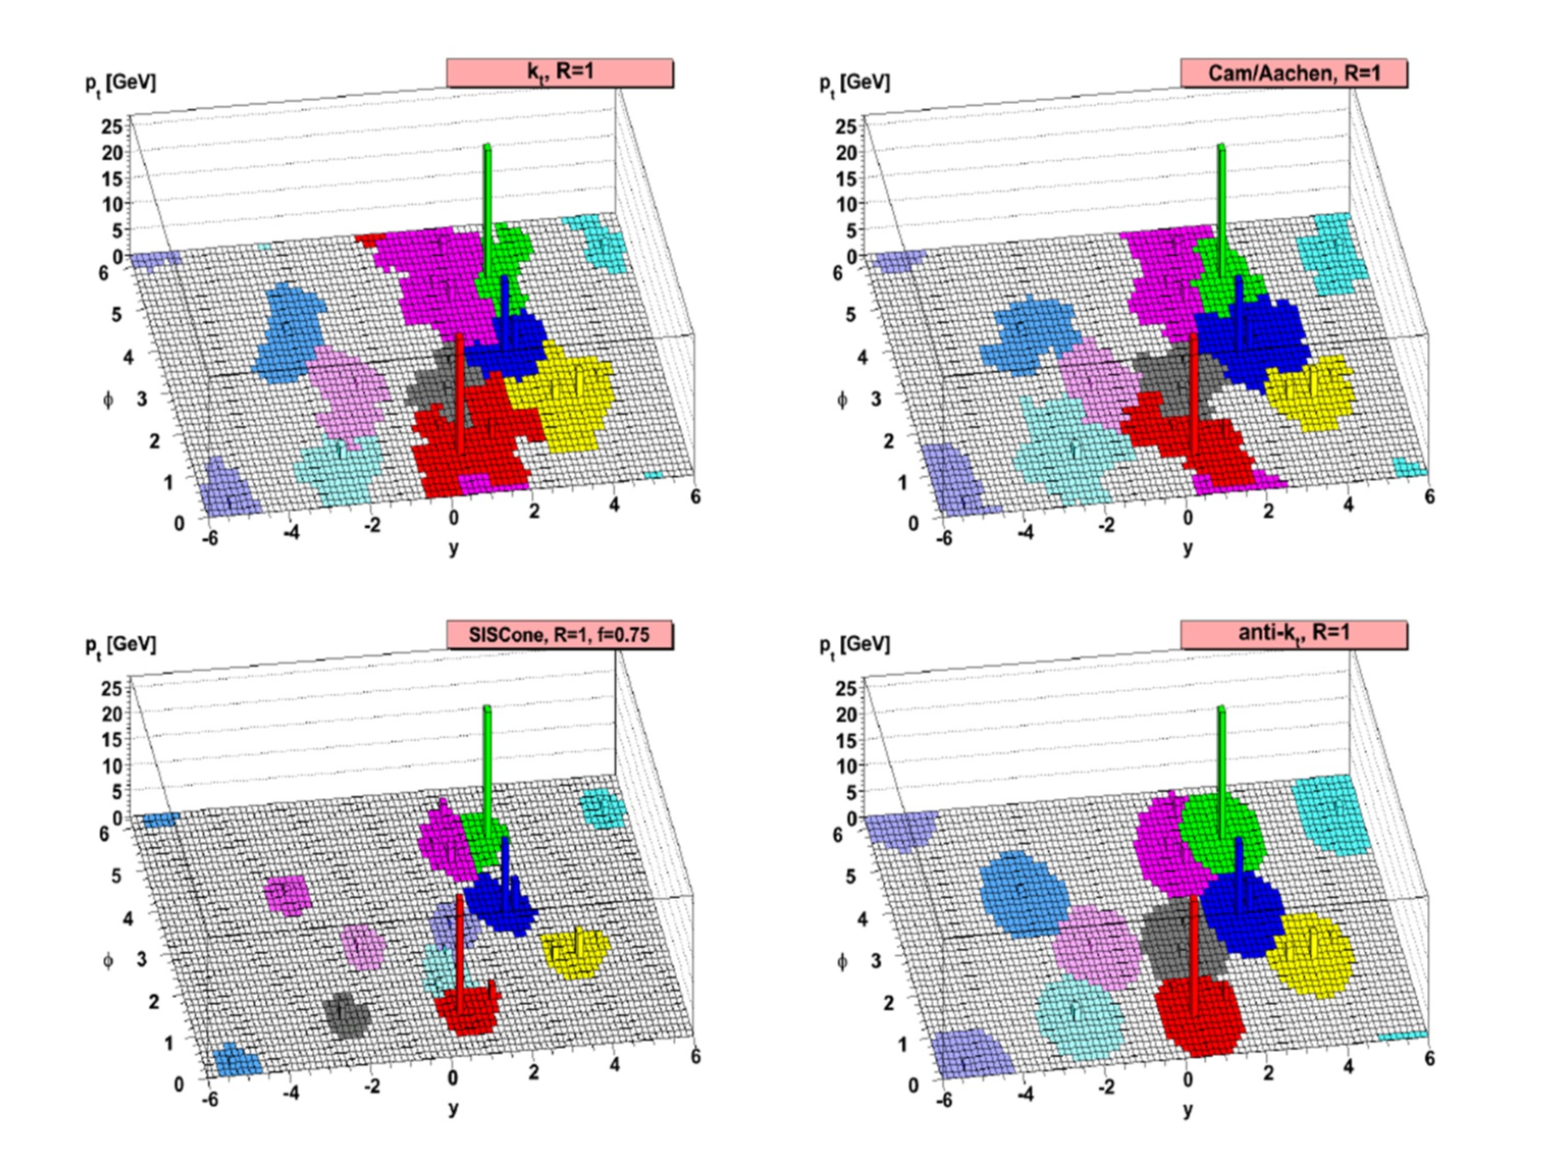
\includegraphics[width=0.9\linewidth]{jet_algo_compare}
\caption{Results of running four different jet clustering algorithm on the same set of parton-level simulated event data.
SISCone (lower-left) is a cone-based algorithm, while the other three are sequential recombination algorithms defined
by different values of $p$~\cite{jet-antikt-algo}.}
\label{fig:jet_algo_compare}
\end{figure}

\section{Jet mass}\label{sec:jet_mass}

As the center-of-mass energy of collisions increases, it becomes increasingly important to study the internal structure of jets, in addition to the kinematic properties of jets within events.
The decay products of hadronically-decaying heavy objects, such as W or Higgs bosons, become harder to resolve into separate jets as the momentum of the original object increases.
Recently, a large number of jet substructure observables have been developed, and an entire subfield has emerged dedicated to the study of the internal properties of jets.

For a two-pronged decay, for example $W \rightarrow q\bar{q}$, the angular separation between the decay products is given by:
\begin{equation}\label{eq:jet_boosted_sep}
    \Delta R = \frac{p_{T}}{2m}
\end{equation}
where $p_T$ is the transverse momentum of the $W$, and $m$ is the $W$ mass.
For $W$ bosons with $p_T \gg m$, jets with radius parameter $R = 0.4$ will no longer resolve the decay products into separate jets,
but instead will contain the all decay products of the $W$ into a single jet.
Figure~\ref{fig:jet_radial_sep} illustrates the boosting effect for the simulated decay $Z'\rightarrow t\bar{t}$, where the $Z'$ represents a new heavy resonance.
Since $m_{Z'} \gg m_{t}$, the top quarks are highly boosted, so their decay products cannot be resolved by jets with $R=0.4$.
On the other hand, jets with $R = 1.0$ will capture all decay products with high efficiency, so the substructure of $R=1.0$ jets can potentially be used to reconstruct these boosted tops.

\begin{figure}[!ht]
    \centering
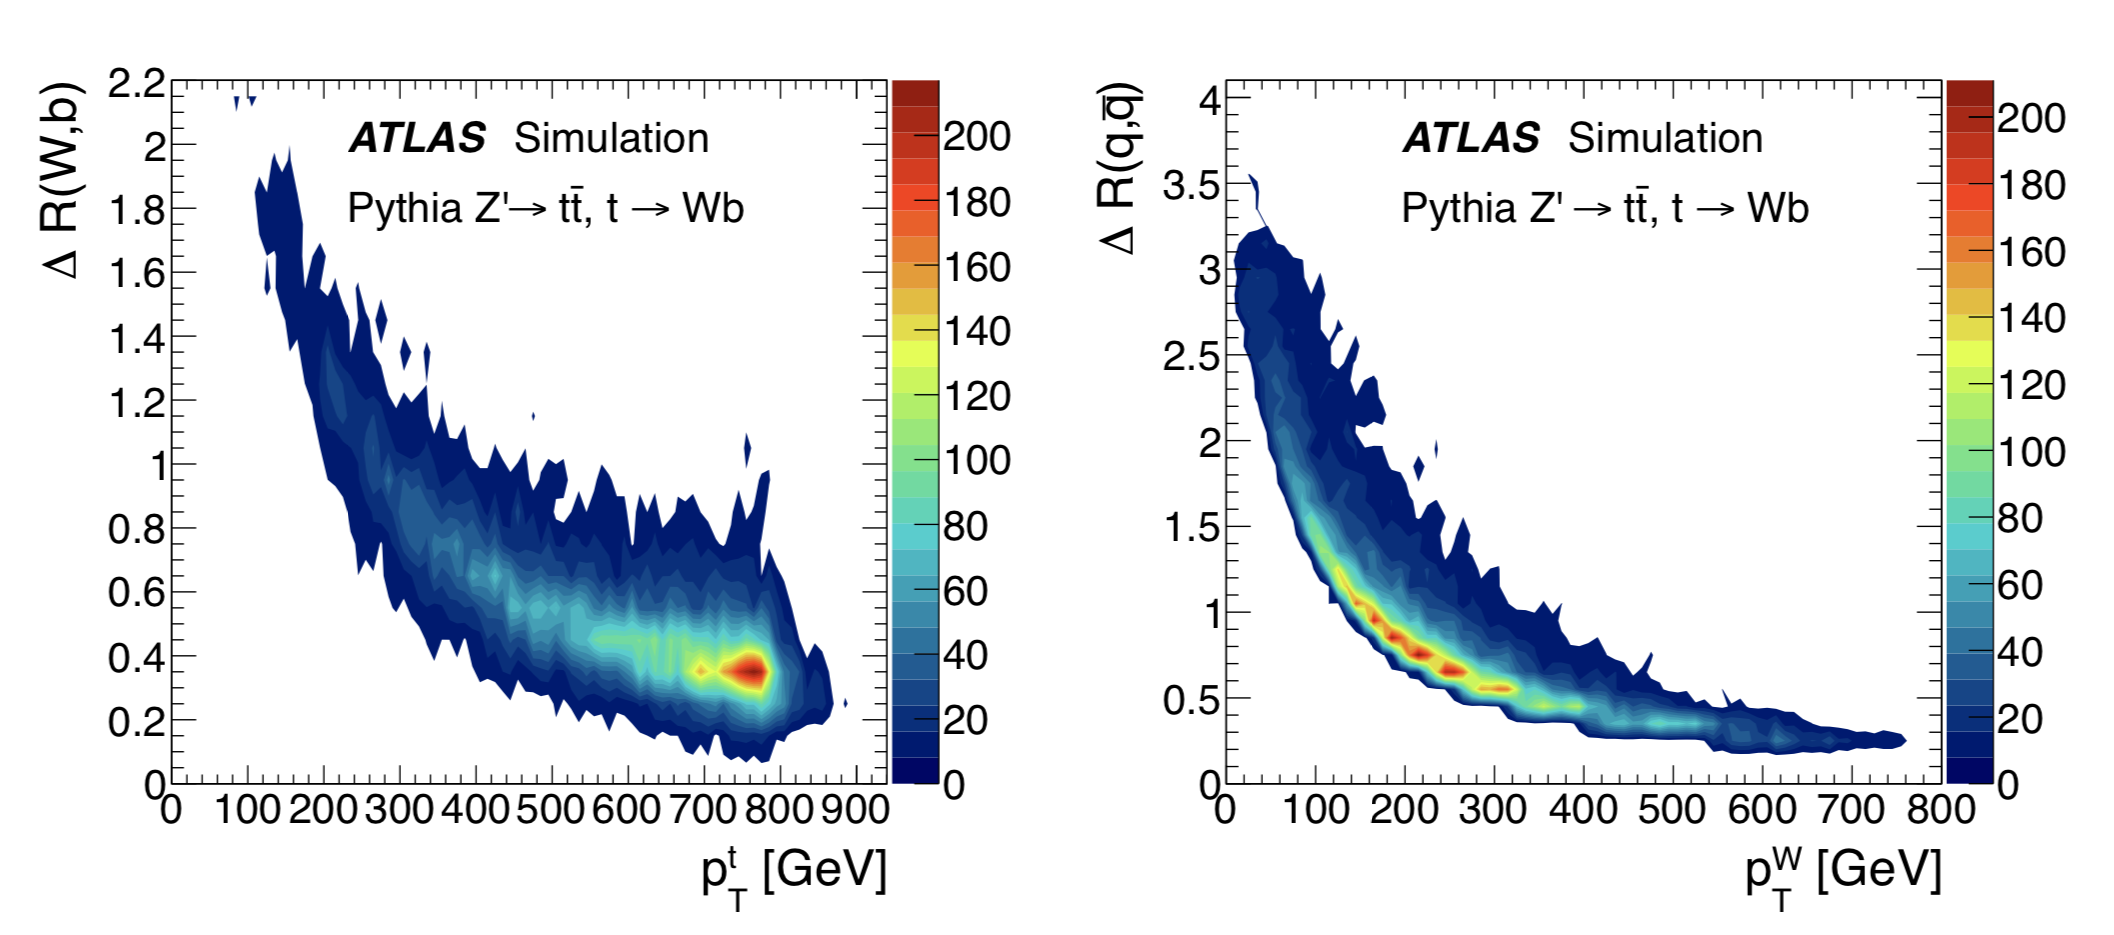
\includegraphics[width=0.6\linewidth]{jet_radial_sep}
\caption{Radial separation between top decay products vs. top-quark $p_T$ for top quarks produced from a theoretical heavy resonance, $Z'$~\cite{jet-substructure-perf}.}
\label{fig:jet_radial_sep}
\end{figure}

When dealing with boosted objects, larger radius parameters are often used, in order to increase the probability of capturing the full decay products of a boosted object.
Jets with large radius parameters, typically $R=1.0$ or $R=1.2$ are referred to as fat jets.

The earliest-developed, and most straightforward jet substructure observable is mass.
The mass of a jet is calculated from the four-vectors of its constituent objects:

\begin{equation}\label{eq:jet_mass}
    m^2 = \left(\sum E_i\right)^2 - \left(\sum \vec{p}_i \right)^2
\end{equation}
For a jet that contains the collimated decay products of an individual boosted resonance, the mass of the jet corresponds to the mass of the resonance, $m_{jet} \approx m_{resonance}$.

For a QCD jet, i.e.\ one that is a result of a high-$p_T$ gluon or light quark, one might expect the mass to also be very low or close to zero.
But in fact perturbative QCD processes lead to a nonzero expected mass for light quark and gluon jets.
Calculations of perturbative QCD jet mass is beyond the scope of this thesis, but the resulting mass is proportional to the jet radius parameter, $R$, and the transverse momentum $p_T$ of the jet.
Jets arising from light quarks will have different mass than jets arising from gluons.
After taking relative production cross-sections for quark and gluon jets into account at different energy scales, the resulting relationship between jet $p_T$ and mass at next-to-leading order (NLO) is well-approximated by~\cite{jet-mass-nlo}:

\begin{equation}\label{eq:jet_mass_nlo}
    m \approx 0.2 p_T R
\end{equation}

Additional contributions to jet mass come from initial state radiation (ISR), pileup (PU), the underlying event (UE), and multi-parton interaction (MPI).
A variety of so-called grooming techniques are used to remove the dependence on this unassociated radiation, so that the groomed jet mass depends only on the mass of the boosted object.
Trimming is a grooming method applied to fat jets after they have been clustered, typically with the anti-$k_T$ algorithm.
Trimming is applied separately to each fat jet, and consists of the following steps:

\begin{enumerate}
    \item Recluster the constituents with a smaller radius parameter, $R_{sub}$, resulting in one or more subjets
    \item Reject any subjet with $p_{T} < f_{cut} p_T^{jet}$
    \item Sum the four-vectors of the subjets that are not rejected to form the final trimmed jet
\end{enumerate}

In the first step, a radius parameter and clustering algorithm must be chosen.
The subjet radius parameter must be smaller than the original radius parameter.
Often, the $k_T$ algorithm is used for subjet clustering, in order to preserve as much of the FSR as possible, because rejecting FSR results in reduced jet mass resolution~\cite{jet-tasi-substructure}.
The values of $R_{sub}$ and $f_{cut}$ can be chosen to reduce pileup sensitivity and maximize jet mass resolution for the signal of interest.
The trimming procedure is illustrated in figure~\ref{fig:jet_trimming}.

\begin{figure}[!ht]
    \centering
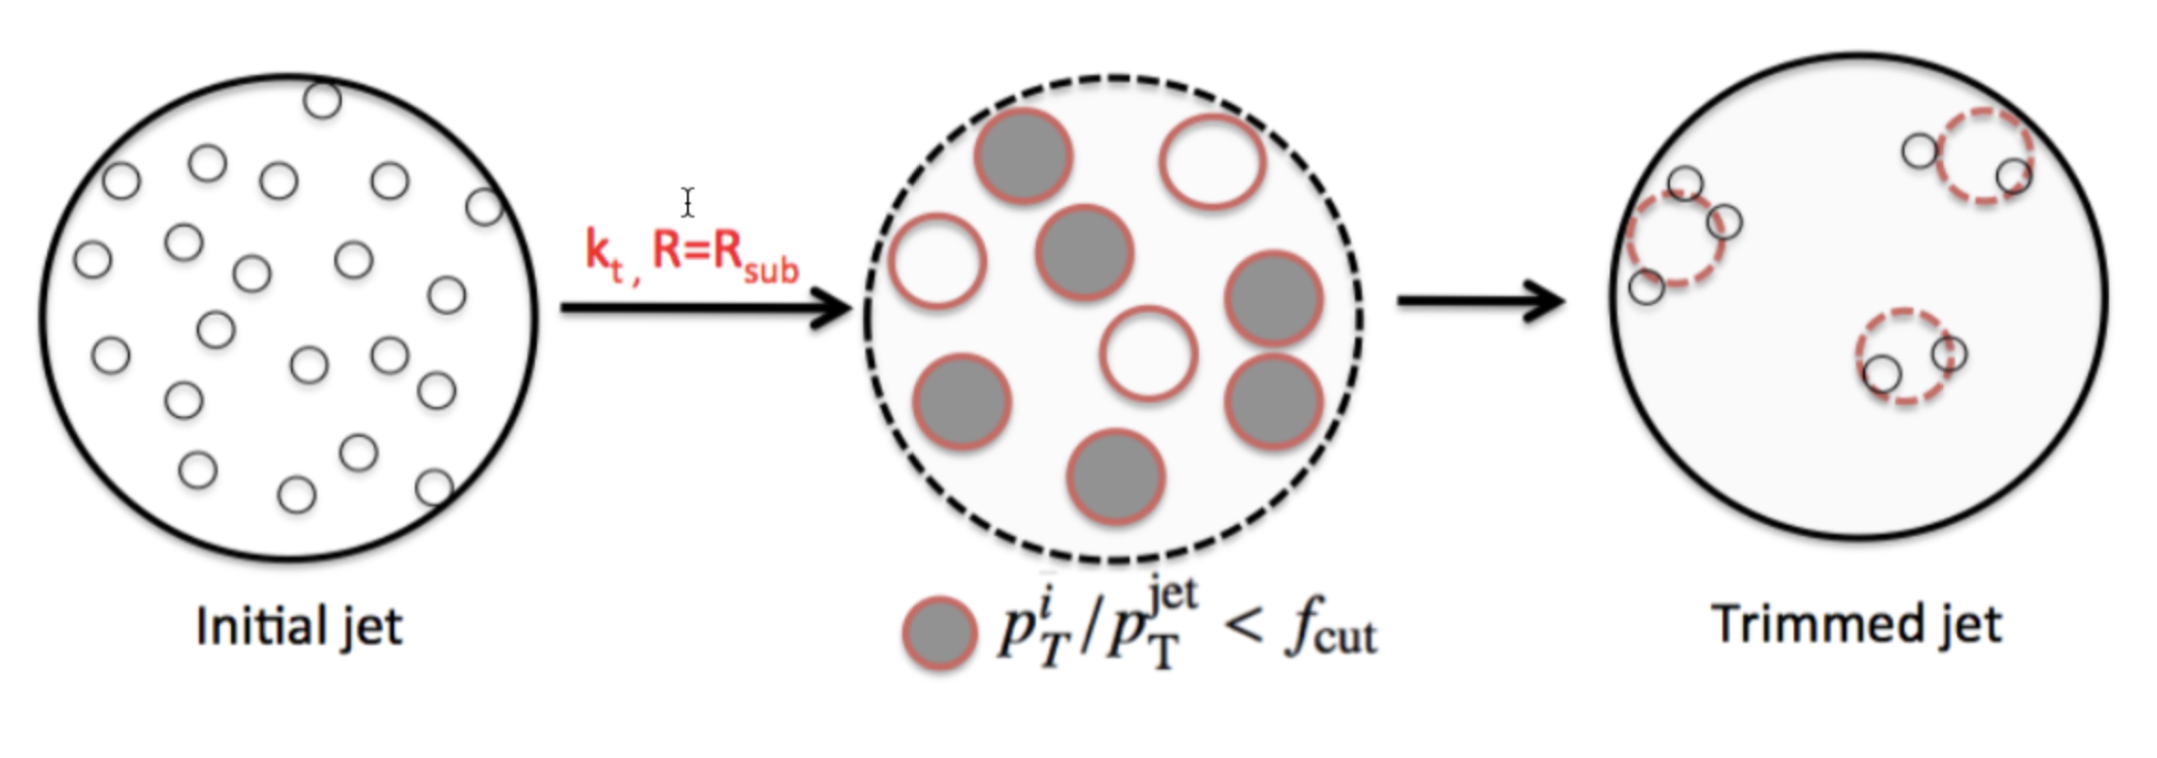
\includegraphics[width=0.9\linewidth]{jet_trimming}
\caption{Illustration of the trimming procedure, one of several grooming methods used to remove the contribution
of unassociated radiation to fat jet mass~\cite{jet-grooming-slides}.}
\label{fig:jet_trimming}
\end{figure}

The effect of different grooming techniques, including trimming, on jet mass resolution can be seen in figure~\ref{fig:jet_grooming_effect}.
For dijet events, high-mass jets are highly suppressed by grooming, which leads to a better signal-to-background ratio for signals of hadronically decaying boosted objects with QCD dijet backgrounds.
For $t\bar{t}$ events, the top-mass peak is somewhat visible before grooming, although much wider than after grooming.
The $W$-mass peak, which is originally completely hidden due to unassociated radiation effects, can be recovered with any of the grooming methods.

\begin{figure}[!ht]
    \centering
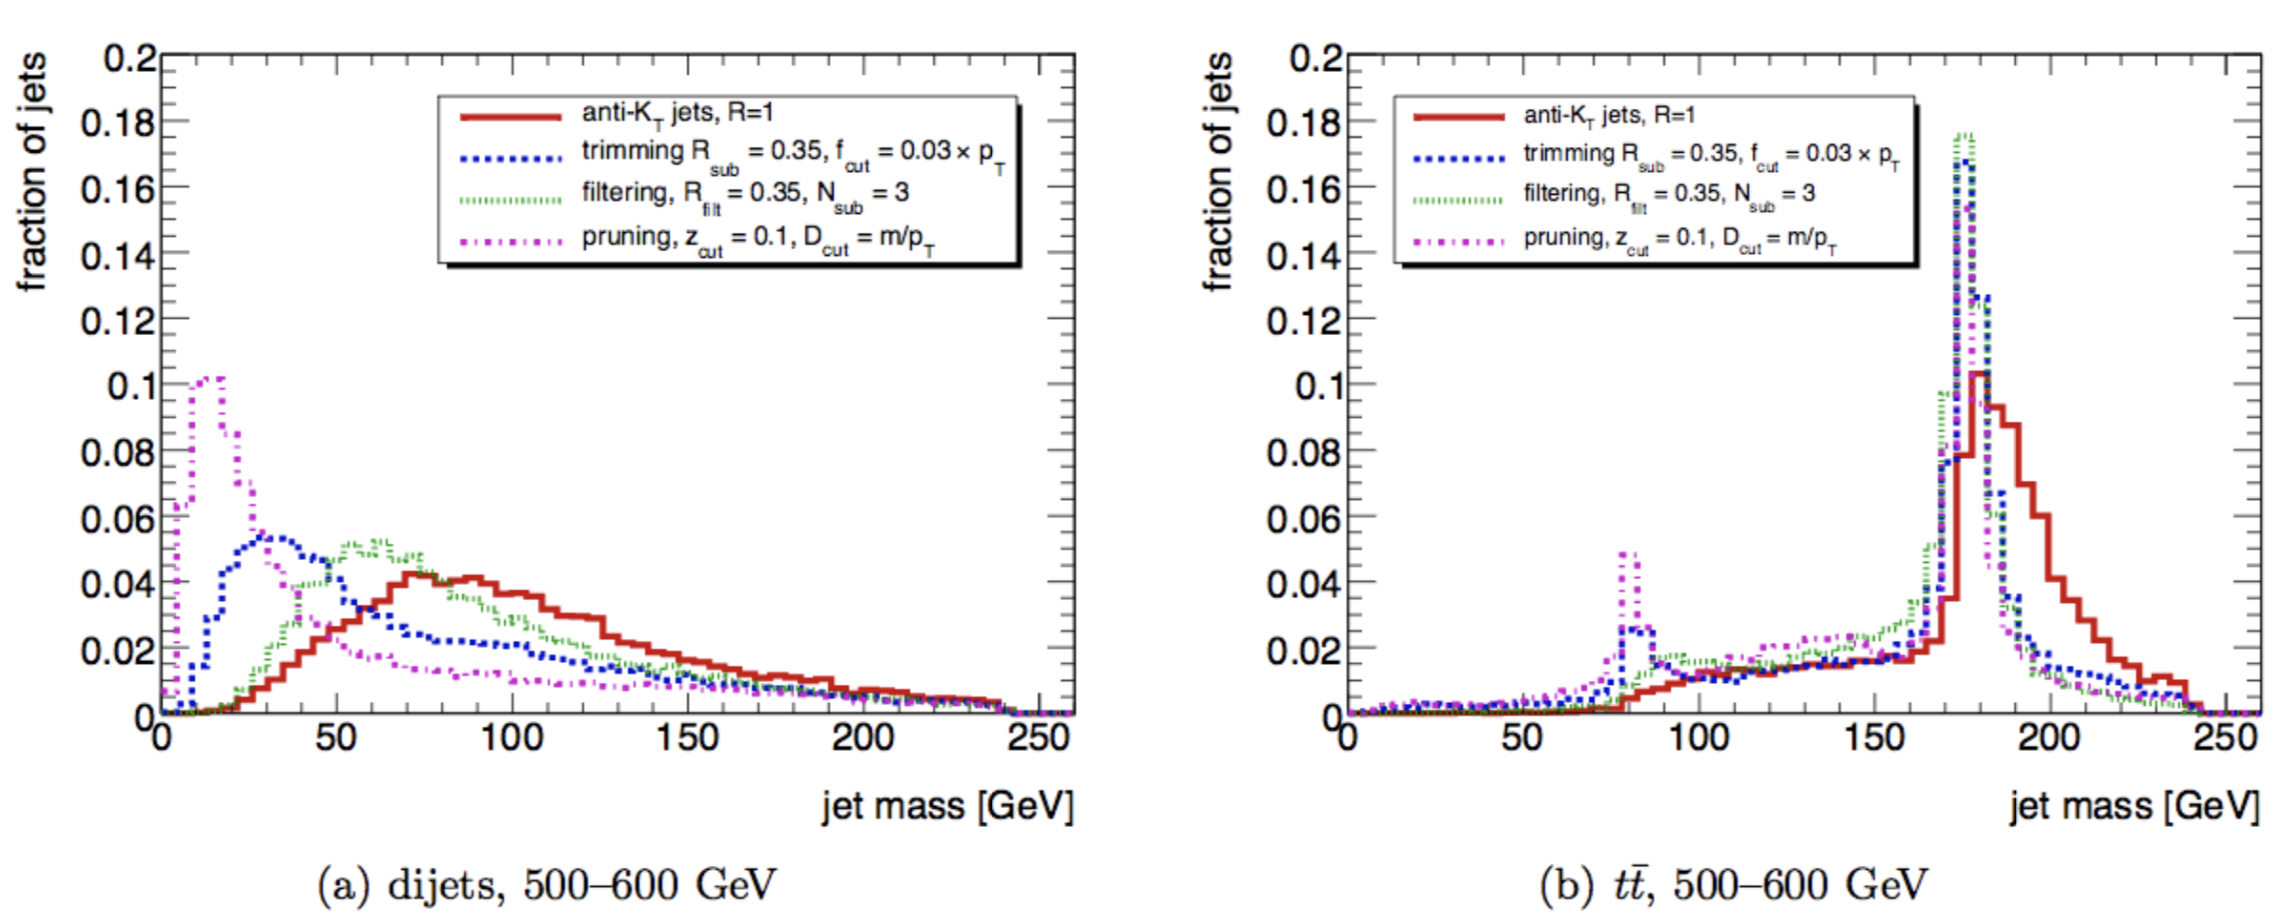
\includegraphics[width=0.9\linewidth]{jet_grooming_effect}
\caption{Jet mass distributions from simulated LHC proton-proton collisions events before and after grooming, for various grooming techniques.
HERWIG is used to simulate $\sqrt{s}=7~TeV$ QCD dijet events (left) and Standard Model $t\bar{t}$ events (right) with parton-level $p_{T}$ between $500$ and $600~GeV$~\cite{jet-boosted}.}
\label{fig:jet_grooming_effect}
\end{figure}

\section{Reconstruction in ATLAS}\label{sec:jet_reconstruction}
The goal of jet measurements in ATLAS is to capture and reconstruct both the energy and momentum of jets leaving the collision point.
Calorimeter jets use clusters of calorimeter cell hits as inputs to the clustering algorithms described in~\ref{sec:jet_clustering}.

\subsection{Topological cell clusters}\label{subsec:jet_topo_clusters}
Topological cell clusters, or topo-clusters, are three-dimensional clusters of calorimeter cell energy measurements.
By clustering groups of calorimeter cells into topo-clusters, the number of inputs to the jet reconstruction algorithm is reduced.
Topo-clustering also reduces calorimeter noise by rejecting cell signals not associated with other nearby significant cell signals~\cite{jet-topo-cluster}.
Topo-clusters serve as the main input to the jet clustering algorithms when reconstructing calorimeter jets in ATLAS .
The two sources of calorimeter cell noise are electronic noise and pileup.

The algorithm is based on the signal-to-noise ratio in each cell, $\zeta_{cell} = E_{cell}/\sigma_{cell}$.
There are three tunable parameters used in the algorithm, labeled $S$, $N$, and $P$, where $S > N \geq P$.
For purposes of the algorithm, a cell is considered to be a \textit{neighbor} of another cell if the two cells are
adjacent in the same layer, or if they are in adjacent layers and have any overlap~\cite{jet-topo-cluster}.

The algorithm is defined as follows:
\begin{enumerate}
    \item Label any cell with $\zeta_{cell}>S$ a seed cell.
    \item Collect all neighboring cells to a seed cell into a proto-cluster.
    \item If any cell in the proto-cluster has $\zeta_{cell}>N$, collect its neighbors into the proto-cluster.
    \item Repeat the previous step until the set of neighbors collected has $\zeta_{cell}<N$.
    \item Reject any cells with $\zeta_{cell}<P$.
\end{enumerate}
At any time in the algorithm, if any cell with $\zeta_{cell}>N$ belongs two proto-clusters, then the two proto-clusters are merged~\cite{jet-topo-cluster}.
Once the algorithm terminates, the final set of topo-clusters are used as the inputs to the desired jet clustering algorithm.

A result of this algorithm is that isolated cells with $\zeta_{cell} < N$ are rejected, which reduces that amount of noise entering the jet clustering algorithm.
These cells are less likely to contain signal than cells with $\zeta_{cell}<N$ that neighbor cells with higher signal-to-noise ratio.
This clustering algorithm does not guarantee that all the energy of a given particle in the jet will be captured by a single topo-cluster, nor does it guarantee that a single topo-cluster only contains energy from a single particle.
So topo-clusters are not measurements of individual particles in the jet.

The three parameters $S$, $N$, and $P$ are tuned on test-beam data with known energy to maximize the measured energy while minimizing the energy resolution\cite{energy-measurement-of-hadrons}.
Results of the test beam energy measurements with $180~GeV$and $20~GeV$ pions can be seen in~\ref{fig:jet_snp_tuning}.
\begin{figure}[!ht]
    \centering
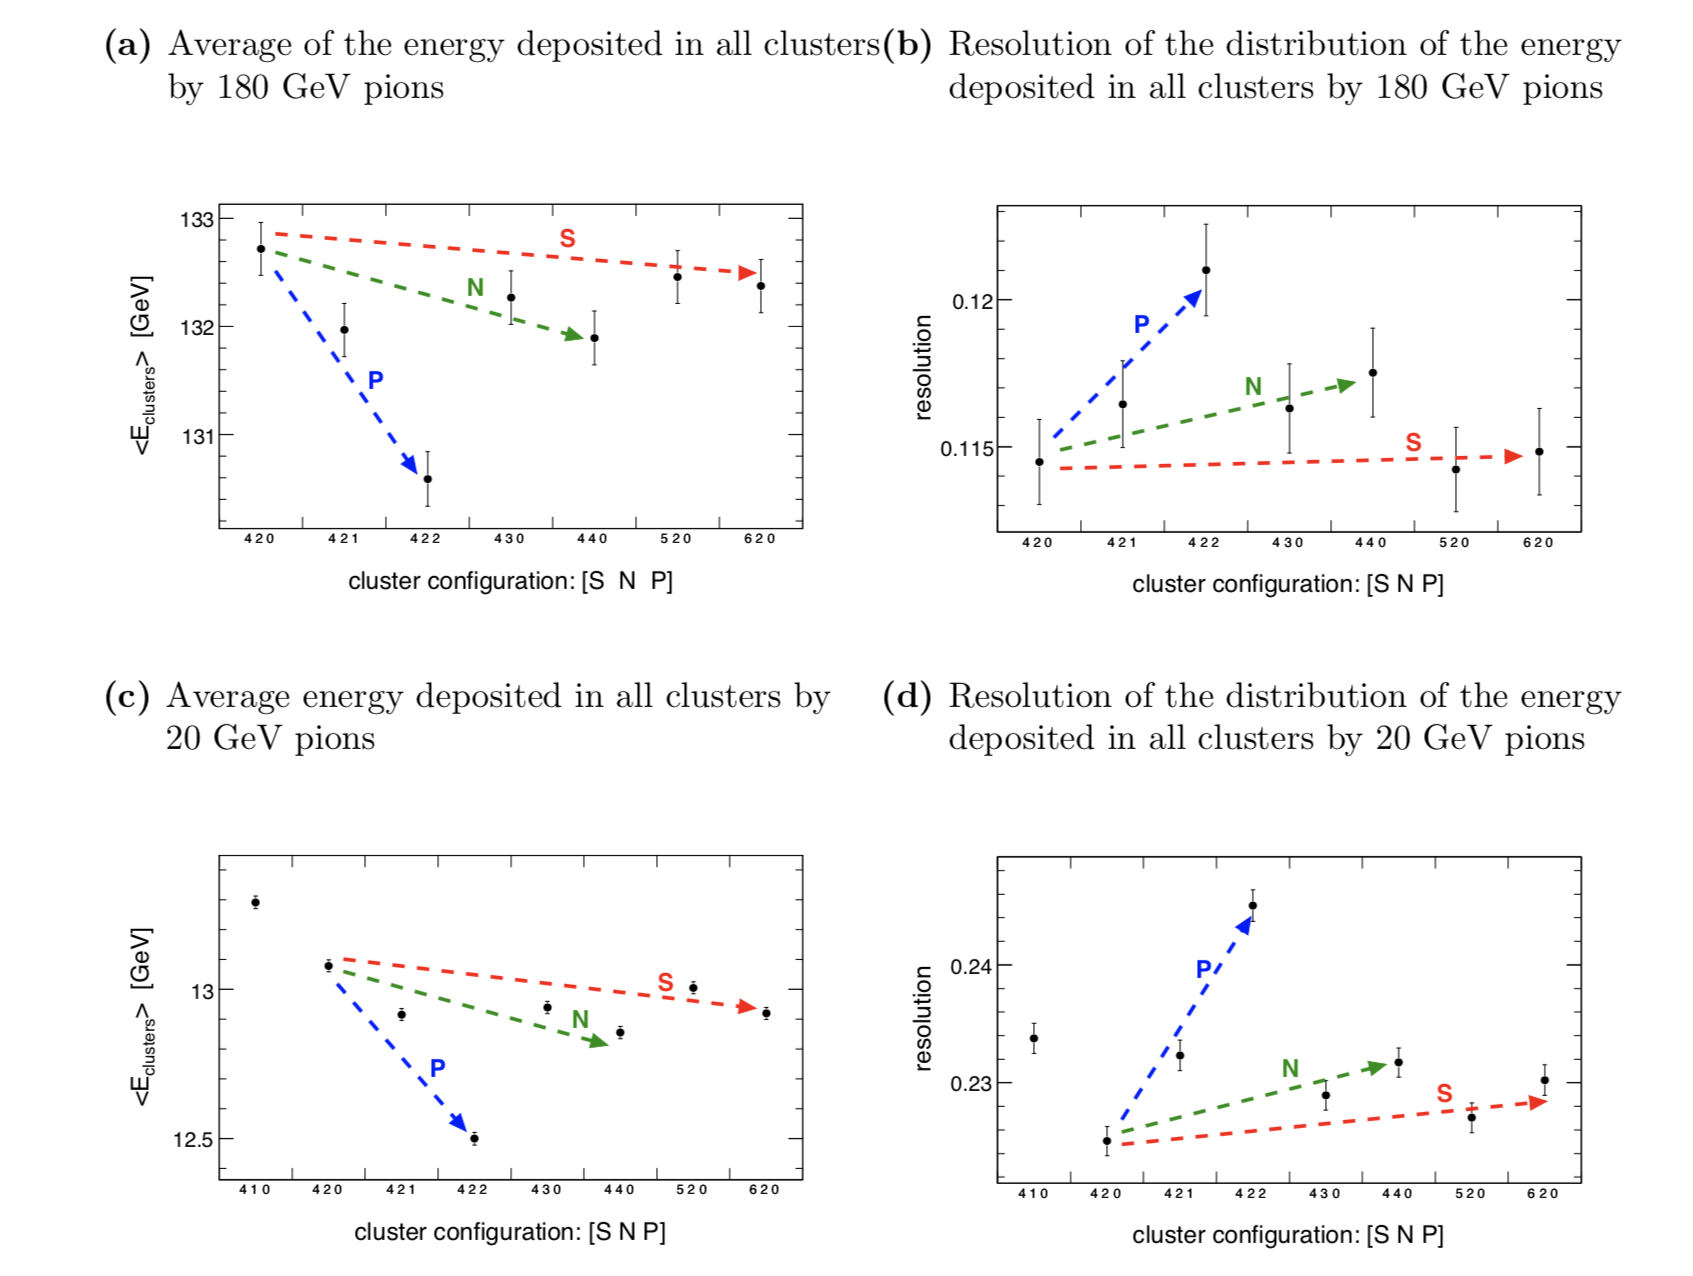
\includegraphics[width=0.9\linewidth]{jet_snp_tuning}
\caption{Average energy and energy resolution measured for $180~GeV$ and $20~GeV$ pions with different values of the
topo-clustering parameters $S$, $N$, and $P$.
The x-axis of each plot represents choices for all three parameters, and the y-axis indicates either the average
energy deposited in each cluster $<E_{clusters}>$ or the energy resolution $RMS/<E_{clusters}>$~\cite{energy-measurement-of-hadrons}.}
\label{fig:jet_snp_tuning}
\end{figure}
Based on these measurements, the default parameter values chosen for ATLAS topo-clustering are $S=4$, $N=2$, $P=0$.
The topo-cluster four momenta are used as the input objects to the jet clustering algorithms.
Other properties of the topo-clusters, known as cluster moments, are used in calibration of the topo-clusters.

\subsection{Topo-cluster calibration}\label{subsec:topo_calibration}

Calibration of topo-clusters is performed before inputting them into the jet clustering algorithms.
Calibration is needed in order to correct for the calorimeters' differing response to electromagnetic and hadronic showers, to correct for signal loss arising from the clustering algorithm, and to account for signal loss due to inactive material.
The calibration strategy known as Local Cell Weighting (LCW) is used to correct for all three of these.
Calibration is done using Monte Carlo simulations of neutral and charged pions in a simulated detector.
Pions with energies up to $2~TeV$ and over a range of $\eta$ values are used.

The ATLAS calorimeters are non-compensating calorimeters, which means they have a lower response for hadronic showers than for electromagnetic showers, for the same energy deposited.
As a result, separate calibrations are needed for hadronic and electromagnetic showers.
A classification algorithm is used to determine the probability that each topo-cluster arose from an electromagnetic shower.
This probability is called $P^{EM}$.
The calibration weight for cell $i$ in cluster $j$ is then:

\begin{equation}\label{eq:lcw_weights}
    w_i = P_{j}^{EM}w_i^{EM}+\left(1-P^{EM}_j\right)w_i^{had}
\end{equation}
where $P_j^{EM}$ is the predicted probability that cluster $j$ arose from an electromagnetic shower, $w_{i}^{EM}$ is the calibration weight for cell $i$ assuming the electromagnetic response, and $w_{i}^{had}$ is the calibration weight for cell $i$ assuming the hadronic response~\cite{jet-topo-cluster}.

Cluster classification probabilities are determined using the topo-cluster depth and signal density, as hadronic showers tend to deposit energy deeper in the calorimeter and have lower energy density~\cite{jet-topo-cluster}.
Figure~\ref{fig:jet_cluster_classification} shows the EM classification probability as a function of these two topo-cluster moments.
The cell signal density is measured as energy density of the cell normalized to the total energy of the cluster to which it belongs.

\begin{figure}[!ht]
    \centering
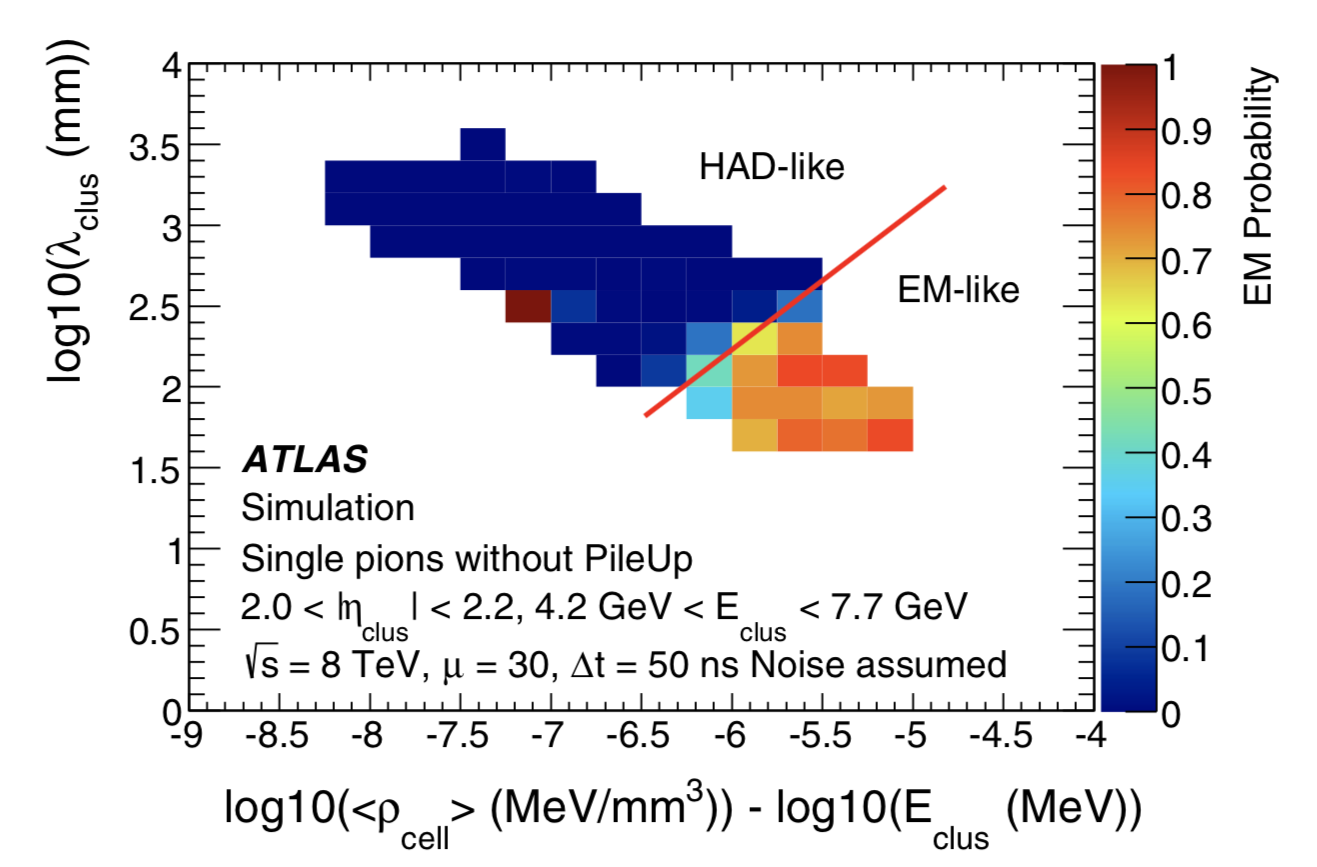
\includegraphics[width=0.9\linewidth]{jet_cluster_classification}
\caption{Cluster EM probability as a function of normalized cell signal density and depth.
Cell that are farther away from their cluster's center, and with lower energy density are more likely to arise
from hadronic showers.
The red line indicates the 50\% boundary: cells falling on that line have a 50\% probability of arising from
electromagnetic showers, while clusters below that line have a higher probability~\cite{jet-topo-cluster}.}
\label{fig:jet_cluster_classification}
\end{figure}
The hadronic calibration weight is then determined as:

\begin{equation}\label{eq:had_cal_weight}
    w_{i}^{had} = \frac{E^{dep}_i}{E^{EM}_i}
\end{equation}
where $E^{dep}_i$ is the true energy deposited in the cell, and $E^{EM}_i$ is the energy measured in the cell.

During the topo-clustering process, cells with signal fractions belows the necessary thresholds can be rejected, resulting in a certain amount of signal energy being lost.
Lost cells with true signal energy deposited are attributed to nearby clusters.
The relevant search area for a cluster depends on the cluster $\eta$, and ranges from $14\deg$ to $60\deg$~\cite{jet-topo-cluster}.
Lost cells can be attributed to more than one cluster, with a weight proportional to the energy deposited in each cluster.
An out-of-cluster correction weight is then calculated as

\begin{equation}\label{eq:out_of_cluster}
    w_{j}^{ooc} = \frac{E_j^{ooc}+E^{dep}_j}{E^{dep}_j}
\end{equation}
where $E_j^{ooc}$ is the total energy deposited in lost cells associated to the cluster, including a fraction
of the energy from lost cells shared by multiple clusters.
This correction is determined separately for electromagnetic and hadronic showers, using neutral and charged pions
respectively\cite{jet-topo-cluster}

Dead material is also accounted for using simulated pions in a simulated detector.
Figure~\ref{fig:jet_lost_cells} shows an illustration of the lost cell and dead material calibration procedure.
\begin{figure}[!ht]
    \centering
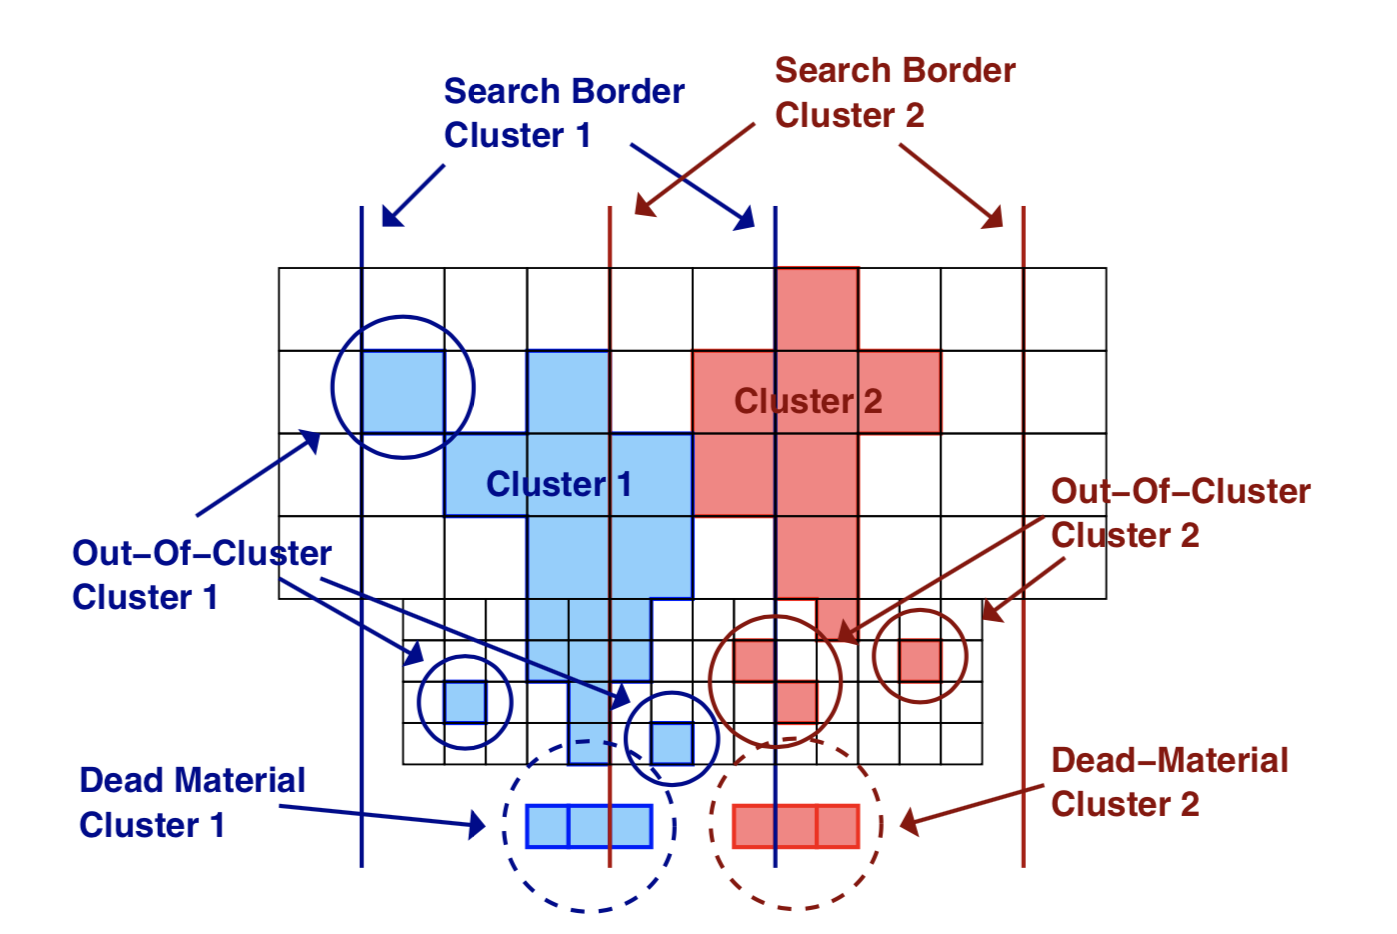
\includegraphics[width=0.9\linewidth]{jet_lost_cells}
\caption{Illustration of the procedure used to account for signal lost to lost cells and dead material~\cite{jet-topo-cluster}.}
\label{fig:jet_lost_cells}
\end{figure}

\subsection{Jet calibration}\label{subsec:jet_calibration}
For large-R jets, the LCW calibration method is applied to topological clusters as described in~\ref{subsec:topo_calibration} before inputting the topo-clusters into the jet clustering algorithm.
After jet clustering, further calibration is required on the resulting jets in order to ensure that the measured energy matches the true energy deposited in the detector.
This is known as the jet energy scale, or JES, calibration.
Several different energy scales are defined in order to describe topo-clusters or jets at different stages in the calibration process.
Those scales are defined as follows:

\begin{itemize}
    \item EM scale: energy as measured directly by the calorimeters
    \item LCW scale: energy after applying the LCW method
    \item EM+JES scale: energy after applying jet-level calibration, if LCW was not used
    \item LCW+JES scale: energy after applying LCW and jet-level calibrations
\end{itemize}

\subsubsection{JES Calibration}\label{subsubsec:jes_calibration}

For the JES calibration of large-R jets, the energy correction procedure described in~\cite{jet-energy-measurement} is applied.
Unlike in~\cite{jet-energy-measurement}, however, the Monte Carlo used for calibration does include pileup.
The reason for this is that large-R jets do not receive a pileup-specific calibration before the JES calibration, unlike standard jets~\cite{jet-substructure-perf}.
The calibration is done by measuring the JES response in bins of true jet energy ($E_{truth}$) and $\eta$.
The response is:

\begin{equation}\label{eq:jet_jes_response}
    \mathcal{R} = E_{meas} / E_{truth}
\end{equation}
For each $\left(E_{truth}, \eta\right)$ bin, the average response $\left<\mathcal{R}\right>$
and average measured energy $\left<E_{meas}\right>$ are measured.
A one-dimensional calibration function $\mathcal{F}_k\left(E_{meas}\right)$ is then obtained by fitting to the distribution of $\left<E_{meas}\right>$ vs. $\left<\mathcal{R}\right>$ in each $\eta$ bin $k$~\cite{jet-energy-measurement}.
Once the calibration functions $\mathcal{F}_k(E_{meas})$ are determined from Monte Carlo, they are applied to jets measured in data.
The calibrated energy for a jet measured with $\eta$ in bin $k$ is:

\begin{equation}\label{eq:jet_jes_calibration}
    E_{calib} = \frac{E_{meas}}{\mathcal{F}_k\left(E_{meas}\right)}
\end{equation}~\cite{jet-energy-measurement}

\subsubsection{JMS Calibration}\label{subsubsec:jms_calibration}

For large-R jets, the jet mass scale (JMS) must be calibrated in addition to the jet energy scale.
A similar procedure to that described in~\ref{subsubsec:jes_calibration} is applied to the JMS calibration, using the jet mass response in place of the jet energy response.
The jet mass response is defined analogously to the jet energy response:

\begin{equation}\label{eq:jet_mass_response}
    \mathcal{R}^{mass} = m_{meas} / m_{true}
\end{equation}
The jet mass response before and after calibration can be seen in figure~\ref{fig:jet_jms_response}.

\begin{figure}[!ht]
    \centering
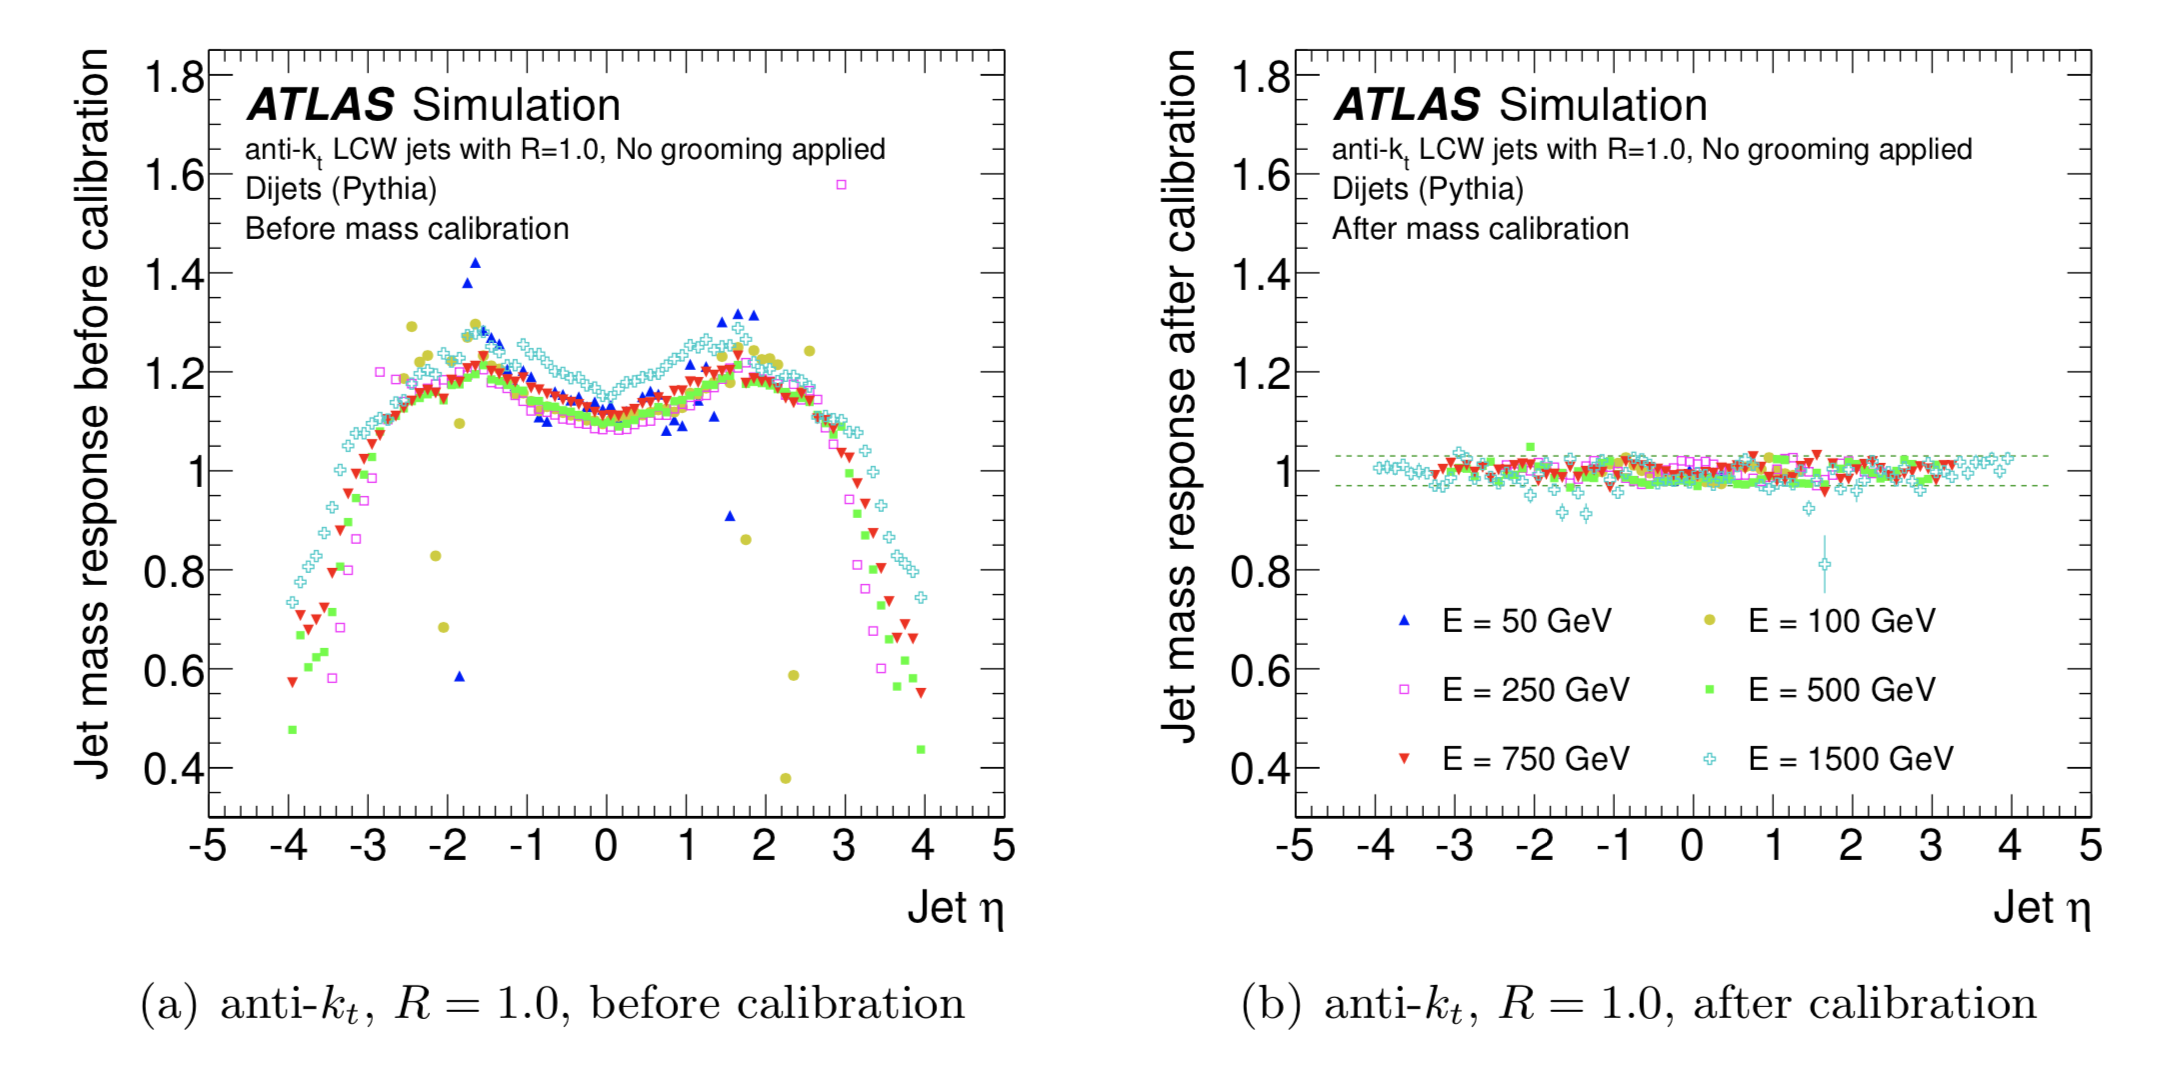
\includegraphics[width=0.9\linewidth]{jet_jms_calibration.png}
\caption{Jet mass response as a function of $\eta$ before and after JMS calibration, for anti-$k_T$ jets
with $R=1.0$ at the LCW scale, without grooming~\cite{jet-substructure-perf}.}
\label{fig:jet_jms_response}
\end{figure}

\subsection{$b$-tagging}\label{subsec:jet_b_tagging}

The identification of jets containing b hadrons, referred to as b-jets, is very important for many different ATLAS physics analyses.
B-tagging is the process of identifying these jets and distinguishing them from jets that do not contain b hadrons.
Jets containing c hadrons can also be distinguished using similar methods.
Jets that don't contain either b hadrons or c hadrons are known as light-flavor jets.
B-tagging and c-tagging are collectively known as flavor tagging.
B-tagging is used in this analysis to suppress the dominant QCD multijet contribution to the background, in order to increase the signal to background ratio.

The main property of b hadrons that allows b-jets to be distinguished from light flavor jets is their relatively long lifetime, on the order of picoseconds.
Because of their long lifetime, b hadrons can travel a measurable distance away from the primary interaction point before decaying.
For example, a $50~GeV$ b hadron will travel an average of $3~mm$ before decaying~\cite{jet-bjet-perf}.
Additionally, b-jets are more likely to contain muons, a fact which can be exploited by b-tagging
algorithms to discriminate between b-jets and light flavor jets~\cite{jet-bjet-perf}.

In this analysis, three different b-tagging algorithms are combined into a multivariate algorithm referred to as MV2.
Each of the three base algorithms uses the relatively large separation distance of b hadron decay vertices away from the primary vertex.

\subsubsection{Impact parameter algorithm}\label{subsubsec:jet_btag_ip}

In the impact parameter algorithms, IP2D and IP3D, individual tracks belonging to a jet are traced back towards the interaction point, and their distance of closest approach to the interaction point, known as the impact parameter, is calculated.
Both the transverse impact parameter, $d_0$, and the longitudinal impact parameter, $z_0 \sin\theta$ are calculated.
Their significances, $d_0/ \sigma_{d_0}$ and $z_0 \sin\theta / \sigma_{z_0 \sin\theta}$ are also calculated.
The IP significances are considered positive if the point of closest approach is on the same side of the primary vertex as the direction of the jet, and negative otherwise.
IP2D uses only transverse IP significance, and IP3D uses both transverse and longitudinal IP significance.
Histograms of the IP significances are calculated using a simulated $t\bar{t}$ sample for b-jets and light flavor jets separately.
These histograms serve as the probability density functions (PDFs) from which a likelihood ratio discriminant is constructed by summing over the likelihood ratios for all tracks in a jet~\cite{jet-bjet-opt}.

Figure~\ref{fig:jet_btag_ip_sig} shows the distribution of transverse and longitudinal impact parameter significances for both heavy quark (b and c) and light quark jets from a simulated $t\bar{t}$ sample.
Large positive IP significances are much more likely to occur for b-jets than for light jets.
Large negative IP significances are more likely to be from noise, and so do not provide good signal discrimination.

\begin{figure}[!ht]
    \centering
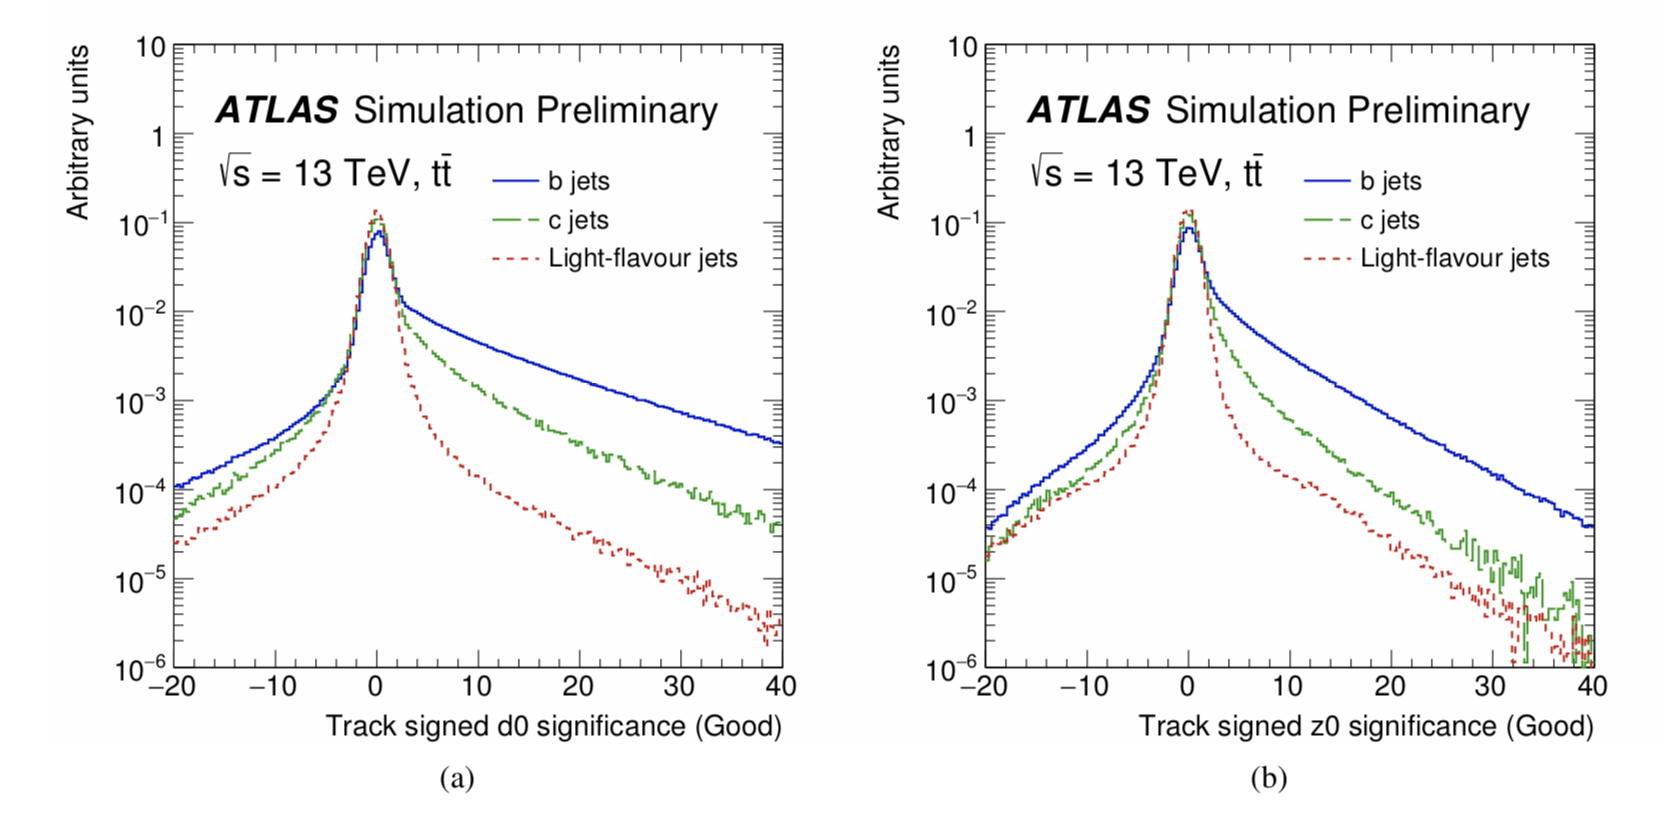
\includegraphics[width=0.9\linewidth]{jet_btag_ip_sig}
\caption{Transverse and longitudinal impact parameter significance distributions for a sample of simulated $t\bar{t}$
events~\cite{jet-bjet-opt}.}
\label{fig:jet_btag_ip_sig}
\end{figure}

\subsubsection{Secondary vertex algorithm}\label{subsubsec:jet_btag_svx}

The secondary vertex algorithm (SVX) also makes use of the long b hadron lifetime and mean flight path.
Rather than calculating impact parameters for individual tracks, multiple tracks are traced back to find where they
intersect other tracks, in order to reconstruct secondary vertices~\cite{jet-commissioning-b-tagging}.
Some filtering is done to reject long-lived particles and other background processes.
Candidate tracks are required to be a certain significant distance from the primary vertex, and the tracks have to pass a goodness-of-fit requirement.
Figure~\ref{fig:jet_btag_svx} shows the secondary vertex reconstruction rate versus jet $p_T$ and jet $\eta$ for b-jets, c-jets, and light flavor jets in a simulated sample of $t\bar{t}$ events.
B-jets are much more likely than light flavor jets to contain a reconstructed secondary vertex that passes all of the selection criteria outlined in~\cite{jet-bjet-opt}.

\begin{figure}[!ht]
    \centering
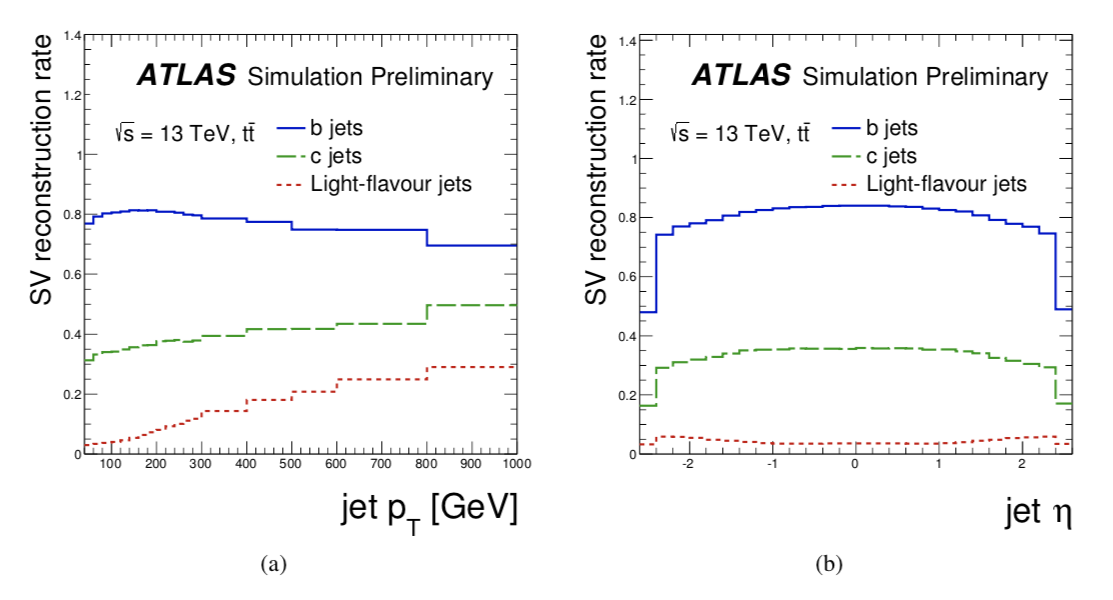
\includegraphics[width=0.9\linewidth]{jet_btag_svx}
\caption{Secondary vertex reconstruction rate versus $p_T$ and $\eta$ for b-jets, c-jets, and light flavor jets
from a simulated sample of $t\bar{t} events$~\cite{jet-bjet-opt}.}
\label{fig:jet_btag_svx}
\end{figure}

\subsubsection{Multi-vertex algorithm}\label{subsubsec:jet_btag_jetfitter}

The third algorithm used to identify b-jets from their mean flight distance from the primary vertex is the multi-vertex reconstruction algorithm, also known as JetFitter.
Rather than reconstruct a single secondary vertex, JetFitter attempts to reconstruct the entire b hadron decay chain~\cite{jet-btag-jetfitter}.
Unlike the SVX algorithm, JetFitter finds multiple vertices that are required to lie in a straight line, along the proposed flight path of the b hadron.
The difference between the SVX and JetFitter algorithm is illustrated in figure~\ref{fig:jet_btag_jetfitter}
\begin{figure}[!ht]
    \centering
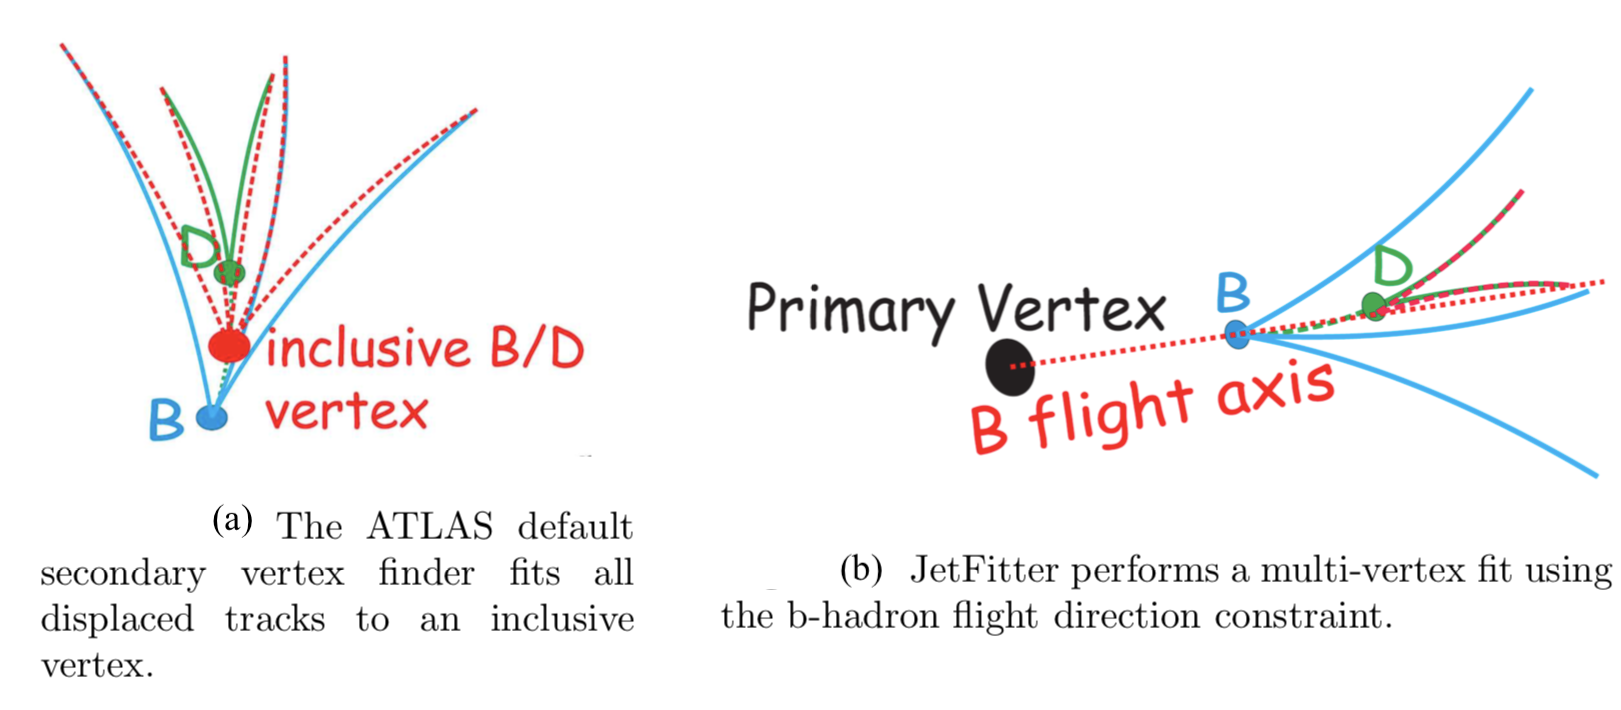
\includegraphics[width=0.9\linewidth]{jet_btag_jetfitter}
\caption{Illustration of the difference between the secondary vertex (a) and multi-vertex (b) algorithms~\cite{jet-btag-jetfitter}.}
\label{fig:jet_btag_jetfitter}
\end{figure}
The efficiency to reconstruct a b hadron decay vertex as a function of jet $p_T$ and $|\eta|$ for b-jets, c-jets, and light flavor jets can be seen in~\ref{fig:jet_btag_jetfitter_perf}
\begin{figure}[!ht]
    \centering
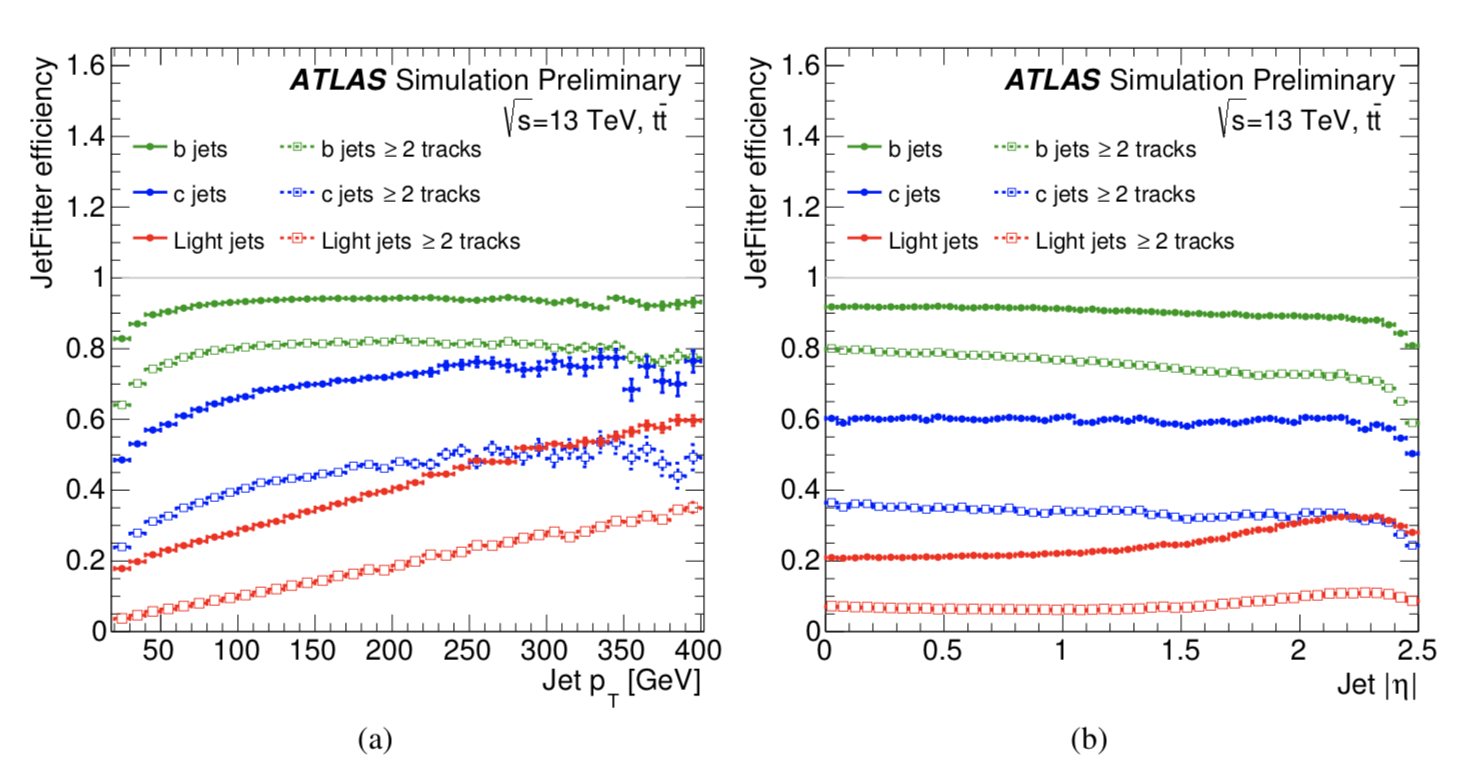
\includegraphics[width=0.9\linewidth]{jet_btag_jetfitter_perf}
\caption{JetFitter vertex reconstruction rate versus $p_T$ and $\eta$ for b-jets, c-jets, and light flavor jets from a simulated sample of $t\bar{t}$ events~\cite{jet-btag-mv2}.}
\label{fig:jet_btag_jetfitter_perf}
\end{figure}

\subsubsection{Multivariate algorithm}\label{subsubsec:jet_btag_mv2}

To get the maximum b-tagging performance, all three of the above mentioned algorithms are combined into a multi-variate algorithm known as MV2.
The algorithm is a boosted decision tree (BDT) which combines the inputs from all three base algorithms mentioned above.
The BDT is trained on a training sample for which b-jets are labeled as signal, and a mixture of light jets and c-jets are labeled as background~\cite{jet-btag-mv2}.
Different versions of the BDT can be obtained by varying the fraction of c-jets and light quark jets in the background training sample.
In this analysis, a mixture of 80\% light quark jets and 20\% c-jets are used in training the BDT, resulting in a discriminant known as MV2c20~\cite{jet-btag-mv2}.
In addition to the inputs from the three base algorithms, MV2 also includes the $p_T$ and $\eta$ of the jet.
There are a total of 24 features input to the BDT, summarized in table~\ref{tbl:jet_btag_mv2_inputs}.
\begin{table}[!ht]
    \centering
\includegraphics[width=0.9\linewidth]{jet_btag_mv2_inputs}
\caption{Description of each of the 24 inputs for the MV2 BDT~\cite{jet-btag-mv2}.}
\label{tbl:jet_btag_mv2_inputs}
\end{table}
The output of the MV2c20 BDT for b-jets, c-jets, and light flavor jets from a simulated sample of $t\bar{t}$ events can be seen in figure~\ref{fig:jet_btag_mv2_output}.

\begin{figure}[!ht]
    \centering
\includegraphics[width=0.6\linewidth]{jet_btag_mv2_output}
\caption{MV2c20 BDT output for b-jets, c-jets, and light flavor jets from a simulated sample of $t\bar{t}$ events~\cite{jet-btag-mv2}.}
\label{fig:jet_btag_mv2_output}
\end{figure}

The BDT reduces the selection criteria from 24 variables to a single one-dimensional discriminant.
The performance of the algorithm in terms of b-tagging efficiency and light flavor jet rejection depends on the choice of threshold value for this discriminant.
Figure~\ref{fig:jet_btag_mv2_eff} shows the b-tagging efficiency versus c-jet and light-jet rejection for the range of MV2 output cut values.
As already  mentioned, MV2c20 is trained with 20\% c-jets in the background sample.
Comparing this to MV2c00, in which only light jets are included in the background training sample, there is clearly improved light-jet rejection by including the c-jets in the background training sample.

\begin{figure}[!ht]
    \centering
\includegraphics[width=0.9\linewidth]{jet_btag_mv2_eff}
\caption{B-tagging efficiency versus light-jet (a) and c-jet (b) rejection for a range of MV2 output cut values.
The red curves are for MV2c20, in which 20\% c-jets are included in the background training sample.
The blue curves are for Mv2c00, which only includes light jets in the background training sample.
The improved c-jet rejection and worsened light-jet rejection can seen by comparing the two~\cite{jet-btag-mv2}.}
\label{fig:jet_btag_mv2_eff}
\end{figure}

In this analysis, the threshold value is chosen such that the b-jet efficiency is 70\%, resulting in a c-jet rejection of 8.1, $\tau$ rejection of 26, and light flavor rejection of 440~\cite{jet-btag-mv2}.
Small-$R$ jets are used in this analysis because the $b$-tagging algorithm is only calibrated for jets with $R=0.4$.

\chapter{Analysis Overview}\label{ch:analysis_overview}

\section{The RPV UDD signature}\label{sec:signal_of_interest}

This analysis is a search for pair-produced gluinos decaying to a large number of standard model quarks via R-parity-violating decays, as described in~\ref{subsec:rpv_gluino}.
In the direct decay model, each gluino decays directly to three standard-model quarks via an effective vertex with an off-shell squark propagator.
In the cascade decay model, each gluino first decays to a neutralino and two quarks, and the neutralino then decays similarly to three quarks vai the RPV effective vertex.
Both types of signal events would result in a large number of high-$p_{T}$ jets in the detector, because they have a large number of quarks in the final state, and each quark must be boosted due to the large mass of the gluinos.
Figure~\ref{fig:analysis_rpv_decays} shows the diagrams for the two signal models under consideration.

\begin{figure}[ht!]
    \centering
\includegraphics[width=0.95\linewidth]{decay_diagrams_combined}
\caption{Diagrams for the two decay processes that are the subject of this search. The direct decay (left) and cascade decay (right)
both involve effective RPV vertices containing off-shell squark propagators.}
\label{fig:analysis_rpv_decays}
\end{figure}

\section{Previous searches and limits}\label{sec:run1_limits}

A similar search was performed using $20.3~fb^{-1}$ of $8~TeV$ ATLAS data from Run 1, and limits were set on the gluino and neutralino masses~\cite{run1-multijet}.
Two different strategies were employed in this analysis.
The first strategy looked for an excess of events with high small-$R$ jet multiplicities.
Signal regions required $\geq6$ or $\geq7$ jets, and different $b$-jet multiplicity requirements were applied to create signal regions sensitive to different heavy-flavor branching fractions.
In the jet-counting analysis, backgrounds were estimated by extrapolating event yields from lower jet multiplicity regions, using a scaling factor derived from multijet Monte Carlo.
This strategy was mainly aimed at the direct-decay model.

The second strategy used the sum of large-$R$ jet masses as discriminating variable, and was mainly aimed at the cascade-decay model.
This strategy derived jet mass templates from signal-depleted control regions, and used those templates to generate the estimated background mass distribution in the signal regions.

For the cascade decay model, the observed limit on the gluino mass ranged from $800~GeV$ to $1~TeV$, depending on the neutralino mass.
Figure~\ref{fig:run1_cascade_limits} shows the $95\%$ CL lower bounds in the $(m_{\tilde{g}}, m_{\tilde{\chi}})$ plane from the search for the cascade-decay signal.
For the direct decay model, different limits were placed on the gluino mass for different assumptions about the flavor composition of the final states.
In the case of light-quark only decays, gluino masses above $917~GeV$ were excluded~\cite{run1-multijet}.
Figure~\ref{fig:run1_direct_limits} shows the $95\%$ CL upper bounds on the cross-section for the direct decay model over a range of gluino masses, for various assumptions about the flavor composition of the final states.

\begin{figure}[!ht]\centering
    \includegraphics[width=0.6\textwidth]{analysis_run1_cascade_limits}
    \caption{Observed and expected limits in the $(m_{\tilde{g}}, m_{\tilde{\chi}})$ plane for the cascade-decay model in ATLAS Run 1 with $\sqrt{s}=8~TeV$~\cite{run1-multijet}.
    }
    \label{fig:run1_cascade_limits}
\end{figure}

\begin{figure}[!ht]\centering
    \includegraphics[width=0.9\textwidth]{analysis_run1_direct_limits}
    \caption{Observed and expected limits on $m_{\tilde{g}})$, along with theoretical cross-section for the direct-decay model in ATLAS Run 1 with $\sqrt{s}=8~TeV$~\cite{run1-multijet}.
    Different limits are set for four different branching fraction scenarios.
    In sub-figure (a), only light-quark decays are allowed.
    In sub-figure (b), each gluino decay results in a top quark in the final state.
    In sub-figure (c), each gluino decay results in a bottom quark in the final state.
    In sub-figure (d), each gluino decay results in both a top and a bottom quark in the final state~\cite{run1-multijet}.}
    \label{fig:run1_direct_limits}
\end{figure}

In Run 1, CMS also performed a search for RPV decays of gluinos with high jet-multiplicity final states~\cite{analysis-cms-run1}.
The analysis assumed that $\lambda''_{tbs}$ is the largest of the UDD coupling constants, motivated by minimal flavor-violating (MFV) SUSY~\cite{susy-mfv}.
Based on this assumption, the analysis specifically looked at the direct-decay model, in which the gluinos each decay to exactly one top, one bottom, and one strange quark, via an off-shell stop.
The analysis looked at events with zero or one-lepton final states high jet multiplicity, using $b$-jet multiplicity as a discriminating variable\cite{analysis-cms-run1}.
For the fully-hadronic channel, the dominant background was QCD multijets, and for the single-lepton channel, the dominant background was from $t\bar{t}$.
In both cases, backgrounds were estimated from Monte Carlo with corrections derived from control-region data.
The single-lepton channel ended up setting the strongest limit on the gluino mass, excluding $pp\rightarrow\tilde{g}\tilde{g}\rightarrow tbs$ for gluinos with mass less than $1.03~TeV$~\cite{analysis-cms-run1}.

The increased luminosity and center-of-mass energy of collisions in Run 2 creates an opportunity to extend the reach of the search for RPV SUSY in multijet final states.
Figure~\ref{fig:results_ten_quark_limits} shows the expected limit for gluino masses under the cascade decay scenario increasing to up to $1.9~TeV$, and up to $1.2~TeV$ under the direct-decay scenario.

\section{Search strategy and discriminating variables}\label{sec:search_strategy}

The search strategy is similar to the total-jet-mass analysis from ATLAS Run 1~\cite{run1-multijet}.
Signal regions include events with a large number of high-mass large-$R$ jets, and backgrounds are estimated using jet mass templates derived from control region data.
The primary discriminating variable is $M_{J}^{\Sigma}$, defined as:

\begin{equation}
    M_{J}^{\Sigma} = \sum_{j=1}^{4}m_{jet}^j
\end{equation}
where $m_{jet}$ is large-$R$ jet mass, and the sum is over the first four highest-$p_{T}$ jets in the event.
Large-$R$ jets are reconstructed with $R=1.0$ and are required to have $p_{T}>200~GeV$ and $|\eta|<2.0$.
In the case where an event has fewer than 4 large-$R$ jets passing the kinematic thresholds, the sum over all large-$R$ jets in the event is used.
This observable is sensitive to the signal because there are large numbers of quarks in the final state, and each quark is likely to have high $p_{T}$ due to the large gluino mass.
Background events, which mainly come from QCD multijet production, tend to have much lower jet mass on average, as explained in~\ref{sec:jet_mass}.
Unlike with the boosted scenarios described in~\ref{sec:jet_mass}, the jet mass for signal events does not come from capturing the decay products of a single boosted heavy object in an individual jet.
Instead, the high jet mass in signal events results from the high probability that two or more decay products, possibly from different parent particles, can accidentally overlap inside the same large-$R$ jet.
$M_{J}^{\Sigma}$ provides good separation between signal and background because it takes into account both the energy and angular structure of an event, unlike a purely energy-dependent observable like $H_{T}$~\cite{hook-mj,elhedri-mj}.
The second discriminating variable is $|\Delta \eta_{12}|$, the pseudorapidity difference between the first two leading jets in an event.

For events with high jet multiplicity, the signal has smaller $|\Delta \eta_{12}|$ than the background.
Distributions of the two discriminating variables are shown in figure~\ref{fig:MJ_dEta_distributions} for data as well as background and signal Monte Carlo.
The different event generators all show similar $M_{J}^{\Sigma}$ distributions for QCD multijets, and a clear difference can be seen between the signal and background distributions.
For signal events, the location of the $M_{J}^{\Sigma}$ peak depends on the gluino mass, moving to higher values for larger masses.
The shape of the $|\Delta \eta_{12}|$ distribution does not depend as strongly on the gluino mass, but there is still a clear difference between the signal and background distributions.
In the analysis, a requirement of small $|\Delta \eta_{12}|<1.4$ can therefore be used to further suppress the background.

\begin{figure}[!ht]
    \centering
    \includegraphics[width=0.9\textwidth]{MJ_dEta_distributions_combined}
    \caption{Distributions of the two main discriminating observables, (a) the scalar sum of the four leading large-R jets, $M_{J}^{\Sigma}$ and (b) the difference in pseudorapidity between the two leading jets, $|\Delta\eta_{12}|$.
    Selected events have $\geq 4$ large-R jets.
    Distributions are shown for both data and simulated signal and background samples.
    The red and green signal distributions are for the cascade decay mode, and the violet distribution is the direct decay mode, for the superpartner masses indicated~\cite{paper-plb}.}
    \label{fig:MJ_dEta_distributions}
\end{figure}

A data-driven method is used to predict the background yield in the signal regions, as well as the uncertainties on those predictions.
The method assumes that for background events, the probably distribution for the mass of an individual jet depends mainly on the $p_{T}$, $\eta$, and flavor of that jet, and does not depend strongly on other details of the event kinematics.
Using this assumption, templates for jet mass can be built from jets in a background-dominated region and used to predict the mass distribution for jets in signal regions.
Templates are binned in $p_{T}$ and $\eta$, and are derived separately for $b$-matched and non-$b$-matched jets.
Each template is the histogram of jet mass within a bin.
The histogram is used as the jet mass probability distribution, conditioned on $p_{T}$, $\eta$, and flavor.
Randomized jet masses, known as dressed masses, are generated from these templates for each jet in the signal region sample.
Summing the dressed masses for each of the up to four leading jets in an event gives the dressed $M_{J}^{\Sigma}$ for that event.
The dressed $M_{J}^{\Sigma}$ distribution for each signal region is used to estimate the expected background contribution to that region.
This method depends on the assumption that the jet mass in background events depends only on $p_{T}$, $\eta$, and flavor.
Independent regions are defined for measuring the extent to which this assumption is violated in data, and this will serve as a systematic uncertainty on the background estimation.
These regions will be called uncertainty determination regions (UDRs).
Background-dominated validation regions will also be defined to test that the dressed $M_{J}^{\Sigma}$ distributions are within the uncertainties derived from the UDRs.

The method is similar to that used in the Run-1 version of the analysis~\cite{run1-multijet}, with a few important differences.
In the Run-1 analysis, the templates were smoothed with a kernel density estimate before sampling the dressed masses.
In this version of the analysis, the templates remain binned.
This allows for an estimate of the statistical uncertainty from the control sample size.
By Poisson fluctuating each template bin before sampling, the statistical uncertainty is propagated to the dressed $M_J^{\Sigma}$ distributions.
Secondly, in the Run-1 version of the analysis, two separate sets of templates were generated: one set for the leading two jets in each event, and a separate set for the third leading jet.
In this analysis, the templates are instead divided into b-matched and non-b-matched jets.
The discrepancy in template shape between b-matched and non-b-matched jets was seen to be larger than that between the third leading jet and first two leading jets.
Finally, the Run-1 version of the analysis used Monte-Carlo non-closure as one contribution to the background systematic uncertainty.
In this analysis, a data-driven method is used instead.
This is due to the fact that the sample size of available simulated data was not large enough to make an accurate estimate of the non-closure.
More details of the template-based background estimation method and how uncertainties are derived from data will be given in~\ref{sec:jet_mass_templates}.

Once the data-driven background estimation and uncertainties have been obtained, a comparison can be done between the observed and expected yields in the signal regions.
If no significant excess is observed, limits can be set on gluino and neutralino masses under the cascade and direct decay model assumptions.
Limits are set by first calculating a 95\% CL upper bound on the signal production cross-section, and then identifying the mass points for which the theoretical cross-section lies outside this bound.
The details of the limit-setting procedure are described in~\ref{sec:results_stats}.

\chapter{Monte Carlo Models of Signal and Background} \label{ch:monte_carlo}

\section{Signal modeling}\label{sec:signal_modeling}

Simulated gluino pair-production events are generated for use in the analysis.
Separate samples are generated for the direct decay and cascade decay models described in~\ref{subsec:rpv_gluino}.
For the direct decay model, events are generated for gluino mass ranging from $900~GeV$ to $1.8~TeV$ .
For the cascade model, the gluino mass is varied from $750~GeV$ up to $2.1~TeV$, with the neutralino mass ranging from $450~GeV$ to $1.9~TeV$ .
For all signal points, the neutralino mass is lower than the gluino mass, as is required by the decay modes of interest.
Signal events are simulated for a discrete set of mass points.
Figure~\ref{fig:signal_cascade_grid} indicates the $\left(m_{\tilde{g}}, m_{\tilde{\chi}_1^0}\right)$ points for which signal evens were generated.
This grid of signal points is chosen to cover the range of masses that the analysis is expected to be sensitive to.
The grid points are spaced closer together in the high-$m_{\tilde{g}}$ region, near where the expected limits (\ref{subsec:results_limits}) lie.

\begin{figure}[!ht]
    \centering

    \includegraphics[width=0.9\linewidth]{signal_cascade_grid}

    \caption{The grid of gluino and neutralino masses for which simulated cascade decay events were generated.
    The triangles indicate the mass points for which simulated events were generated.}

    \label{fig:signal_cascade_grid}
\end{figure}

\subsection{Event generation}\label{subsec:signal_event_gen}

Matrix elements for gluino pair production are generated with \textsc{MadGraph\_aMC@NLO} v2.3.3, which is a convenient framework for calculating arbitrary matrix elements at up to next-to-leading order (NLO)~\cite{signal-madgraph}.
\textsc{MadGraph} allows the user to specify the theory being used and values for the free parameters, then it constructs and calculates the necessary Feynman diagrams.
In this analysis, matrix elements are calculated at leading order (LO).
In the pair-production matrix elements, up two two additional partons are allowed to be produced along with the gluino pair.

To model the parts of the collision environment described in section~\ref{sec:jet_collisions}, such as the underlying event, parton shower, and fragmentation, \textsc{Pythia} 8.186 is used~\cite{signal-pythia}.
Interfacing \textsc{MadGraph} and \textsc{Pythia} is made possible by a standardized file format known as Les Houches Event Format (LHEF)~\cite{signal-lhef}.

As discussed in section~\ref{sec:jet_collisions}, there are non-perturbative processes that occur in proton-proton collisions, which cannot be directly calculated from first principles.
This processes can be parameterized and approximated in a program like \textsc{Pythia}, requiring many free parameters with values that must be constrained using data.
The process of inferring these parameters so that the calculations match the data is known as tuning.
For this analysis the A14 set of tuned parameter values~\cite{signal-pythia-a14,signal-pythia-tunes} and the NNPDF2.3LO set~\cite{signal-nnpdf} of PDFs are used to model the underlying event in~\textsc{Pythia}.
EvtGen v1.2.0~\cite{mc-evtgen} is used for modelling b- and c-hadron decays.

\subsection{Cross-section}\label{subsec:signal_cross_section}
In order to estimate the expected signal yield and uncertainty, the nominal production cross section and its uncertainty must be known.
Gluino pair-production cross-sections have been calculated at a range of center-of-mass energies, and the results are summarized in~\cite{signal-xsec}.
The gluino pair-production cross-section and its uncertainty over a range of gluino masses can be seen in~\ref{fig:signal_xsec}.
The uncertainty band comes from calculating the cross section with different PDF sets and with different factorization and renormalization scales~\cite{signal-xsec}.
\begin{figure}[!ht]\centering
    \includegraphics[width=0.9\linewidth]{signal_xsec}
    \caption{Gluino pair-production cross-section and uncertainty for $\sqrt{13}~TeV$ proton-proton collisions at the LHC, calculated at NLO+NLL~\cite{signal-xsec}.}
    \label{fig:signal_xsec}
\end{figure}

\subsection{Fast simulation with Atlfast-II}\label{subsec:fastsim}

Simulation of the detector response to physics events requires large amounts of computational resources.
In order to reduce the cost of generating large samples of simulated events, a faster version of the detector response simulation, called Atlfast-II has been developed~\cite{mc-atlfast}.
Fast simulation with Atlfast-II (AFII) can greatly reduce the time required to generate these simulated events, but makes several simplifications that can lead to less precise results.

A comparison between the full detector simulation (FullSim) and AFII was performed to find out if using AFII would reduce the sensitivity of the search or otherwise affect the analysis.
Very good agreement between FullSim and AFII-simulated events is observed across a range of kinematic observables relevant to this analysis.
As a result, AFII simulation is used for generating signal events for all of the grid points used in the limit-setting.
Full simulation events are also generated for a few representative signal points.

For the FullSim/AFII comparison, full simulation events for the decay modes described in chapter~\ref{ch:analysis_overview} are not available, but a very similar signal is used.
In this case, pair-produced gluinos each decay to a neutralino + $t\bar{t}$, and the neutralinos each decay through a $\lambda''$ vertex to three light quarks.
This process is illustrated in~\ref{fig:mc_gtt}.
The benchmark model used in this study has $m_{\tilde{g}}=1250~GeV$ and $m_{\tilde{\chi}}=450~GeV$.
Events used in this study are required to have $H_{T}>1~TeV$ and lead jet $p_{T}>200~GeV$.
Large-$R$ jets are fully calibrated using FullSim calibration and required to have $p_{T}$ of at least $100~GeV$ and $|\eta|$ less than $2.8$.
Jet mass response is defined as $m_{reco}/m_{truth}$, where $m_{reco}$ is the reconstructed jet mass and $m_{truth}$ is the mass of jets clustered from truth particles.

Figure~\ref{fig:afii_mass_response} shows the large-$R$ jet mass response vs. truth mass and vs. truth $p_{T}$ for large-$R$ jets with $p_{T}>100~GeV$ and $|\eta|<2.8$.
The points and error bars show the best-fit mean and width for a Gaussian fit to the core of the distribution in each bin.
Figure~\ref{fig:afii_kinematics} shows the distribution of large-$R$ jet kinematic observables $m$, $\eta$, $\phi$, and $p_{T}$ for both FullSim and AFII, along with the ratio of each bin in the bottom panel of each plot.
Figure~\ref{fig:afii_mj} shows the large-$R$ jet multiplicity histogram for reconstructed jets using both AFII and FullSim, and the distributions of $M_{J}^{\Sigma}$ for events with at least 5 large-$R$ jets.
In all cases, very good agreement is observed between FullSim and AFII distributions.

\begin{figure}[!ht]\centering
    \includegraphics[width=0.6\linewidth]{mc_gtt}
    \caption{The process used for the AFII/FullSim comparison study.
    The signal is very similar to the cascade decay model used in the search, but the gluinos decay to a neutralino+$t\bar{t}$ rather than a neutralino and two light quarks.}
    \label{fig:mc_gtt}
\end{figure}

\begin{figure}[!ht]\centering
    \includegraphics[width=0.9\linewidth]{mc_afII_mass_response}
    \caption{Jet mass response vs true jet mass (left) and truth jet $p_{T}$ for simulated signal events using both the full detector simulation (full sim) and Atlfast-II (fast sim).
    Points and error bars show the best-fit mean and width for a Gaussian fit to the core of the distribution in each bin.
    The model used for this study is similar to the cascade decay model described in~\ref{ch:analysis_overview}, except each gluino decays to a neutralino + $t\bar{t}$ rather than a neutralino and two light quarks.
    The gluino mass is $1250~GeV$ and neutralino mass is $450~GeV$.
    Jets are required to have $p_{T}$ greater than $100~GeV$ and $|\eta|<2.8$.
    }
    \label{fig:afii_mass_response}
\end{figure}

\begin{figure}[!ht]\centering
    \includegraphics[width=0.9\linewidth]{mc_afii_kinematics}
    \caption{Kinematic distributions of large-$R$ jets for simulated events using both the full detector simulation (full sim) and Atlfast-II (fast sim).
    The model used for this study is similar to the cascade decay model described in~\ref{ch:analysis_overview}, except each gluino decays to a neutralino + $t\bar{t}$ rather than a neutralino and two light quarks.
    The gluino mass is $1250~GeV$ and neutralino mass is $450~GeV$.
    Jets are required to have $p_{T}$ greater than $100~GeV$ and $|\eta|<2.8$.
    }
    \label{fig:afii_kinematics}
\end{figure}

\begin{figure}[!ht]\centering
    \includegraphics[width=0.9\linewidth]{mc_afii_mj}
    \caption{Jet multiplicity and distribution (left) and $M_{J}^{\Sigma}$ for events with at least 5 large-$R$ jets (right) for simulated events using both the full detector simulation (full sim) and Atlfast-II (fast sim).
    The model used for this study is similar to the cascade decay model described in~\ref{ch:analysis_overview}, except each gluino decays to a neutralino + $t\bar{t}$ rather than a neutralino and two light quarks.
    The gluino mass is $1250~GeV$ and neutralino mass is $450~GeV$.
    Jets are required to have $p_{T}$ greater than $100~GeV$ and $|\eta|<2.8$.}
    \label{fig:afii_mj}
\end{figure}

\section{Background modeling}\label{sec:bkg_modeling}

Background estimation for this analysis is done with a fully data-driven method that does not rely on Monte Carlo to make predictions.
However, simulated background events are generated and studied in order to test and validate the data-driven background estimation method.
This process is detailed in~\ref{sec:bkg_monte_carlo}.

The Pythia8 multijet background sample is generated using Pythia8 8.186~\cite{signal-pythia}.
Like with the signal samples described in~\ref{subsec:signal_event_gen}, the A14 underlying-event tune~\cite{signal-pythia,signal-pythia-a14} and the NNPDF2.3LO PDF sets are used~\cite{signal-nnpdf}.
Multijet samples are also generated with Sherpa and Herwig++.
The $t\bar{t}$ events are generated with Powheg-Box v2~\cite{mc-powheg} with the CT10 PDF set~\cite{mc-ct10-pdf}.

The differential multijet cross section falls drastically with increasing $p_{T}$, so multijet events are not generated with a probability distribution proportional to the differential cross section.
If they were, the result would be enormous numbers of events with only low-$p_{T}$ jets, and very few events with high-$p_{T}$, resulting in very large statistical uncertainties for the high-$p_{T}$ jet events.
Instead, multijet events are generated in slices, where each slice has a minimum requirement on the leading-jet $p_{T}$.
Approximately equal numbers of events can then be generated for each slice, and re-weighted according to the relative cross-section of each slice.
Using this method, the statistical uncertainty is more constant across a wide range of jet $p_{T}$.
The lowest-$p_{T}$ slice that passes the event selection for this analysis has a lead-jet range of $160~GeV - 400~GeV$.
For this slice, just under 16 million simulated events are generated, which corresponds to an effective luminosity of $1.9~fb^{-1}$.
\chapter{Data Sample, Event Selection, and Jet Definitions}\label{ch:data_and_event_selection}

\section{Data sample}\label{sec:data}
This analysis uses the entirety of the 2015 and 2016 ATLAS datasets, comprising \linebreak $36.1~fb^{-1}~(\pm2.1\%)$ of integrated luminosity, with $\sqrt{s}=13~TeV$.
A \textit{good runs list} (GRL) is used to select only those data-taking periods in which alld detectors are fully functional~\cite{data-grl}.

\section{Trigger}\label{sec:trigger}
Events are required to pass an $H_{T}$-based trigger, where $H_{T}$ is the scalar sum of the $p_{T}$ of all jets in an event.
The jets used for the calculation of $H_{T}$ in the trigger are level-one jets with $p_{T}>100~GeV$.
To pass the trigger, an event must have $H_{T}>1~TeV$.
Figure~\ref{fig:trigger_efficiency} shows the trigger efficiency versus large-$R$ jet $p_{T}$ threshold for events with $\geq4$ and $\geq5$ large-$R$ jets.
For events with five or more large-$R$ jets, the trigger efficiency is $100\%$ when the jet $p_{T}$ threshold is $200~GeV$ or above.
For events with four or more jets, an additional requirement on the leading jet $p_{T}$ is needed to ensure full trigger efficiency at this jet-$p_{T}$ threshold.
For the $\geq4$-jet regions, the leading jet will be required to have a $p_{T}$ of at least $440~GeV$.

\begin{figure}[!ht]
    \centering
    \includegraphics[width=0.9\textwidth]{data_trigger_efficiency}
    \caption{Trigger efficiency versus large-$R$ jet $p_{T}$ threshold for events with $\geq4$ and $\geq5$ large-$R$ jets.
    For events with $\geq4$ large-$R$ jets, and additional requirement of leading-jet $p_{T}>400~GeV$ ensures $100\%$ trigger efficiency.
    }
    \label{fig:trigger_efficiency}
\end{figure}

\section{Event selection}\label{sec:event_selection}

Events considered by this analysis must meet the following pre-selection criteria:

\begin{itemize}
    \item In the list of good luminosity blocks in the GRL as described in~\ref{sec:data}.
    \item No errors in the LAr or tile calorimeters or the inner detector when the events were measured
    \item Pass the $H_{T}$ trigger as described in~\ref{sec:trigger}.
    \item At least one primary vertex from at least two tracks with $p_{T}>400~MeV$ each
    \item At least one large-$R$ jet (see~\ref{sec:jet_definitions}) with $p_{T}>440~GeV$
\end{itemize}

\section{Jet definitions, $b$-tagging, and $b$-matching}\label{sec:jet_definitions}

In this analysis, two different types of jets are defined.
Large-$R$ jets are reconstructed using the anti-$k_{T}$ algorithm with $R=1.0$ and are trimmed by re-clustering the constituents of each jet with $R_{sub-jet}=0.2$ and rejecting any sub-jet with $p_{T}^{sub-jet}/p_{T}^{jet}<0.05$.
The trimmed large-$R$ jets are required to have $p_{T}>200~GeV$.

Small-$R$ jets are reconstructed using the anti-$k_{T}$ algorithm with $R=0.4$.
To be considered for b-tagging, a small-R jet must have $p_{T}$ of at least $50~GeV$ and $|\eta|$ less than $2.5$.
The fixed-efficiency $70\%$ working point is used for $b$-tagging.

Only large-$R$ jets are used for the analysis, but the $b$-tagging algorithm is only calibrated for small-$R$ jets.
So a matching procedure is used to identify large-$R$ jets that can be associated with a $b$-tagged small-$R$ jet.
Large-$R$ jets found to be within $\Delta R=1.0$ of a $b$-tagged small-$R$ jet in the same event are referred to as $b$-matched jets.
Jet mass templates are derived separately for $b$-matched and non-$b$-matched jets.

For details of how jets are reconstructed, trimmed, and calibrated, as well as the definition of different jet parameters, see chapter~\ref{ch:jets}.
The algorithm used to identify $b$-jets is described in chapter~\ref{subsec:jet_b_tagging} as well as~\cite{b-jet-perf-1,b-jet-perf-2}.

The control, validation, and signal regions defined in section~\ref{sec:region_defs} can be segmented into $b$-tag and $b$-veto regions.
Events with at least one $b$-tagged small-$R$ jet are considered $b$-tag events, while those without are labelled as $b$-veto.
When $b$-tagging is not part of the selection requirements for a region, it is called a $b$-inclusive region.

\section{Control, signal, validation, and uncertainty determination regions} \label{sec:region_defs}
Events are divided into control, signal, validation, and uncertainty determination regions.
Figure~\ref{fig:workflow} illustrates how the different regions are used in the analysis.
Jet mass templates are constructed from control region (CR) events and used predict the mass distribution in the uncertainty determination region (UDR), validation region (VR), and signal region (SR), as discussed in section~\ref{sec:jet_mass_templates}.
The discrepancy between predicted and observed jet masses in the UDR is taken as the systematic uncertainty of the background estimation method.
Observed and predicted masses in the validation regions can be compared to check that any discrepancy falls within this uncertainty, as a way of validating the method.
Finally the observed yields in the signal region can be compared to the predicted background yield in the signal region.

\begin{figure}[!ht]
    \centering
    \includegraphics[width=0.9\textwidth]{background_workflow}
    \caption{Workflow illustrating how the different regions are used in the analysis.}
    \label{fig:workflow}
\end{figure}

Table~\ref{tbl:region_defs} gives the cuts used to define each of these regions.
Control region events are required to have exactly three large-$R$ jets each with $p_{T}>200~GeV$.
If a control region event has at least one $b$-matched large-$R$ jet, the additional requirement of $|\Delta\eta_{12}|>1.4$ is applied, in order to suppress potential signal contamination.

There are a total of five partially-overlapping signal regions, all of which require $|\Delta\eta_{12}|<1.4$.
Regions are defined by the minimum number of large-$R$ jets required ($N_{jet}$), by whether or not a $b$-tagged jet is required to be present in the event, and by a minimum requirement on $M_{J}^{\Sigma}$.
There are two signal regions which require four or more large-$R$ jets with $p_{T}>200~GeV$, and three signal regions which require five or more.
Four-jet signal regions require the $p_T$ of the leading large-$R$ jet to be greater than $400~GeV$.
The $b$-tag signal regions each require at least one $b$-tagged small-$R$ jet per event, and are the most sensitive to the RPV gluino direct and cascade decay models.
Signal regions without the $b$-tag requirement are also defined, referred to as inclusive signal regions.
These inclusive regions are less sensitive to the RPV gluino decay signal, but can be sensitive to other potential BSM signals.

The minimum value of $M_{J}^{\Sigma}$ for each signal region is optimized based on signal sensitivity separately for each signal region.
For the 5-jet $b$-tag signal region, the optimal $M_{J}^{\Sigma}$ cut is $0.8~TeV$ for the cascade decay model, and $0.6~TeV$ for the direct decay model.
The signal regions corresponding to these two $M_{J}^{\Sigma}$ cuts will be referred to as 5jSRb1 and 5jSRb2, respectively.

The difference between the signal and validation regions is a reversal of the $|\Delta\eta_{12}|$ requirement, and removal of the $M_{J}^{\Sigma}$ requirement.
Requiring large $|\Delta\eta|_{12}$ reduces the signal contribution to these high-multiplicity regions.
There is no $M_{J}^{\Sigma}$ requirement for the validation region, so that the performance of the template method over the full range of $M_{J}^{\Sigma}$ can be evaluated.

There are two uncertainty determination regions (UDRs), which are used to derive the data-driven background systematic uncertainty.
The high-$p_{T}$ UDR, referred to as as UDR1, consists of events with exactly two large-R jets, with at least one having $p_{T}>400~GeV$.
The low-$p_{T}$ UDR, referred to as UDR2, consists of events with exactly four large-R jets, all of which have $p_{T}<400~GeV$.
The UDRs are independent of the control, validation, and signal regions.

\begin{table}
    \centering

    \begin{tabular}{cccccccc}

        \toprule
                             &                        & $N_{jet}~(p_T>200~GeV)$ & $b$-tag & $b$-match & $p_{T,1}$  & $|\Delta\eta_{12}|$ & $M_{J}^{\Sigma}$ \\
        \midrule
        \multirow{2}{*}{CR}  & 3jCRb                  & $=3$                    & -       & Yes       & -          & -                   & - \\
                             & 3jCR                   & $=3$                    & -       & No        & -          & -                   & - \\
        \midrule
        \multirow{2}{*}{UDR} & UDR1                   & $=2$                    & -       & -         & $>400~GeV$ & -                   & - \\
                             & UDR2                   & $=4$                    & -       & -         & $<400~GeV$ & -                   & - \\
        \midrule
        \multirow{4}{*}{VR}  & 4jVRb                  & $\geq4$                 & Yes     & -         & $>400~GeV$ & $>1.4$              & - \\
                             & 5jVRb                  & $\geq5$                 & Yes     & -         & -          & $>1.4$              & - \\
                             & 4jVR                   & $\geq4$                 & -       & -         & $>400~GeV$ & $>1.4$              & - \\
                             & 5jVR                   & $\geq5$                 & -       & -         & -          & $>1.4$              & - \\
        \hline
        \multirow{5}{*}{SR}  & 4jSRb                  & $\geq4$                 & Yes     & -         & $>400~GeV$ & $<1.4$              & $>1.0~TeV$ \\
                             & \multirow{2}{*}{5jSRb} & $\geq5$                 & Yes     & -         & -          & $<1.4$              & $>0.8~TeV$ \\
                             &                        & $\geq5$                 & Yes     & -         & -          & $<1.4$              & $>0.6~TeV$ \\
                             & 4jSR                   & $\geq4$                 & -       & -         & $>400~GeV$ & $<1.4$              & $>1.0~TeV$ \\
                             & 5jSR                   & $\geq5$                 & -       & -         & -          & $<1.4$              & $>0.8~TeV$ \\
        \bottomrule
    \end{tabular}

    \caption{Summary of the requirements defining the control, uncertainty determination, validation, and signal regions.
    Requirements are placed on the large-R jet multiplicity ($N_{jet}$), the presence or absence of a b-tagged small-R jet ($b$-tag),
    the $p_T$ of the leading jet ($p_{T,1}$), the pseudorapidity difference between the two leading jets ($|\Delta\eta_{12}|$),
    and the scalar sum of the first four leading jets in the event ($M_J^{\Sigma}$)~\cite{paper-plb}.}
    \label{tbl:region_defs}

\end{table}

\chapter{Background estimation method}\label{ch:background_method}

\section{Control, signal, validation, and uncertainty determination regions} \label{sec:region_defs}
Events are divided into control, signal, validation, and uncertainty determination regions.
Figure~\ref{fig:workflow} illustrates how the different regions are used in the analysis.
Jet mass templates are constructed from control region (CR) events and used predict the mass distribution in the uncertainty determination region (UDR), validation region (VR), and signal region (SR), as discussed in section~\ref{sec:jet_mass_templates}.
The discrepancy between predicted and observed jet masses in the UDR is taken as the systematic uncertainty of the background estimation method.
Observed and predicted masses in the validation regions can be compared to check that any discrepancy falls within this uncertainty, as a way of validating the method.
Finally the observed yields in the signal region can be compared to the predicted background yield in the signal region.

\begin{figure}[!ht]
    \centering
    \includegraphics[width=0.9\textwidth]{background_workflow}
    \caption{Workflow illustrating how the different regions are used in the analysis.}
    \label{fig:workflow}
\end{figure}

Table~\ref{tbl:region_defs} gives the cuts used to define each of these regions.
Control region events are required to have exactly three large-$R$ jets each with $p_{T}>200~GeV$.
If a control region event has at least one $b$-matched large-$R$ jet, the additional requirement of $|\Delta\eta_{12}|>1.4$ is applied, in order to suppress potential signal contamination.

There are a total of five partially-overlapping signal regions, all of which require $|\Delta\eta_{12}|<1.4$.
Regions are defined by the minimum number of large-$R$ jets required ($N_{jet}$), by whether or not a $b$-tagged jet is required to be present in the event, and by a minimum requirement on $M_{J}^{\Sigma}$.
There are two signal regions which require four or more large-$R$ jets with $p_{T}>200~GeV$, and three signal regions which require five or more.
Four-jet signal regions require the $p_T$ of the leading large-$R$ jet to be greater than $400~GeV$.
The $b$-tag signal regions each require at least one $b$-tagged small-$R$ jet per event, and are the most sensitive to the RPV gluino direct and cascade decay models.
Signal regions without the $b$-tag requirement are also defined, referred to as inclusive signal regions.
These inclusive regions are less sensitive to the RPV gluino decay signal, but can be sensitive to other potential BSM signals.

The minimum value of $M_{J}^{\Sigma}$ for each signal region is optimized based on signal sensitivity separately for each signal region.
For the 5-jet $b$-tag signal region, the optimal $M_{J}^{\Sigma}$ cut is $0.8~TeV$ for the cascade decay model, and $0.6~TeV$ for the direct decay model.
The signal regions corresponding to these two $M_{J}^{\Sigma}$ cuts will be referred to as 5jSRb1 and 5jSRb2, respectively.

The difference between the signal and validation regions is a reversal of the $|\Delta\eta_{12}|$ requirement, and removal of the $M_{J}^{\Sigma}$ requirement.
Requiring large $|\Delta\eta|_{12}$ reduces the signal contribution to these high-multiplicity regions.
There is no $M_{J}^{\Sigma}$ requirement for the validation region, so that the performance of the template method over the full range of $M_{J}^{\Sigma}$ can be evaluated.

There are two uncertainty determination regions (UDRs), which are used to derive the data-driven background systematic uncertainty.
The high-$p_{T}$ UDR, referred to as as UDR1, consists of events with exactly two large-R jets, with at least one having $p_{T}>400~GeV$.
The low-$p_{T}$ UDR, referred to as UDR2, consists of events with exactly four large-R jets, all of which have $p_{T}<400~GeV$.
The UDRs are independent of the control, validation, and signal regions.

\begin{table}
    \centering

    \begin{tabular}{cccccccc}

        \toprule
                             &                        & $N_{jet}~(p_T>200~GeV)$ & $b$-tag & $b$-match & $p_{T,1}$  & $|\Delta\eta_{12}|$ & $M_{J}^{\Sigma}$ \\
        \midrule
        \multirow{2}{*}{CR}  & 3jCRb                  & $=3$                    & -       & Yes       & -          & -                   & - \\
                             & 3jCR                   & $=3$                    & -       & No        & -          & -                   & - \\
        \midrule
        \multirow{2}{*}{UDR} & UDR1                   & $=2$                    & -       & -         & $>400~GeV$ & -                   & - \\
                             & UDR2                   & $=4$                    & -       & -         & $<400~GeV$ & -                   & - \\
        \midrule
        \multirow{4}{*}{VR}  & 4jVRb                  & $\geq4$                 & Yes     & -         & $>400~GeV$ & $>1.4$              & - \\
                             & 5jVRb                  & $\geq5$                 & Yes     & -         & -          & $>1.4$              & - \\
                             & 4jVR                   & $\geq4$                 & -       & -         & $>400~GeV$ & $>1.4$              & - \\
                             & 5jVR                   & $\geq5$                 & -       & -         & -          & $>1.4$              & - \\
        \hline
        \multirow{5}{*}{SR}  & 4jSRb                  & $\geq4$                 & Yes     & -         & $>400~GeV$ & $<1.4$              & $>1.0~TeV$ \\
                             & \multirow{2}{*}{5jSRb} & $\geq5$                 & Yes     & -         & -          & $<1.4$              & $>0.8~TeV$ \\
                             &                        & $\geq5$                 & Yes     & -         & -          & $<1.4$              & $>0.6~TeV$ \\
                             & 4jSR                   & $\geq4$                 & -       & -         & $>400~GeV$ & $<1.4$              & $>1.0~TeV$ \\
                             & 5jSR                   & $\geq5$                 & -       & -         & -          & $<1.4$              & $>0.8~TeV$ \\
        \bottomrule
    \end{tabular}

    \caption{Summary of the requirements defining the control, uncertainty determination, validation, and signal regions.
    Requirements are placed on the large-R jet multiplicity ($N_{jet}$), the presence or absence of a b-tagged small-R jet ($b$-tag),
    the $p_T$ of the leading jet ($p_{T,1}$), the pseudorapidity difference between the two leading jets ($|\Delta\eta_{12}|$),
    and the scalar sum of the first four leading jets in the event ($M_J^{\Sigma}$)~\cite{paper-plb}.}
    \label{tbl:region_defs}

\end{table}

\section{Jet mass templates}\label{sec:jet_mass_templates}

\subsection{Template creation}\label{subsec:template_creation}

Jet mass templates are derived from a signal-depleted control region consisting of events with exactly three large-R jets.
For each $p_T$, $|\eta|$, and b-match bin, the distribution of individual jet masses in that bin is taken as the template.
The templates combine to form the binned conditional probability distribution: $p(m|p_{T}, |\eta|, b-match)$.

Separate templates are created for b-matched and non-b-matched jets.
For the b-matched templates, only events with $|\Delta \eta_{1,2}| > 1.4$ are included in the templates.
Templates derived from b-matched jets are used to dress b-matched jets in the kinematic sample,
and templates derived from non-b-matched jets are used to dress non-b-matched jets in the kinematic sample.
Each template is a one-dimensional histogram of $\log\left(m/p_{T}\right)$, with $50$ bins.
Jets with $\log\left(m/p_{T}\right)< -7$ are excluded from the templates.
Example templates are shown in figure~\ref{fig:template_examples} for two representative $p_{T}$-$|\eta|$ bins.
A clear difference can be seen between the templates derived from b-matched and non-b-matched jets.
Jets that are b-matched have a higher value of $m/p_{T}$ than non-b-matched jets, for the same  $p_{T}$-$|\eta|$ bin.
This feature can be seen in both data and simulation.
Additionally, agreement between data and simulation is observed in the general template shapes.

\begin{figure}[!ht]
    \centering
    \includegraphics[width=0.9\textwidth]{template_examples}
    \caption{Two representative template distributions used in the analysis, showing a comparison between data in black and simulation in red.
    The solid markers show the templates derived from b-matched jets, while the empty markers show the templates derived from non-b-matched jets.
    In (a), template jets are required to have $600~GeV < p_{T} < 644~GeV$ and $0.5 <|\eta|<1.0$.
    In (b), templates jets are required to have $733~GeV < p_{T} < 811~GeV$ and $1.5<|\eta|<2.0$~\cite{paper-plb}.}
    \label{fig:template_examples}
\end{figure}

Templates are binned in $p_T$ and $|\eta|$.
The $p_T$ bins are approximately logarithmic, while the $|\eta|$ bin boundaries are at $0.0$, $0.5$, $1.0$, and $1.5$.
The template binning and number of jets contributing to each bin are shown in figure~\ref{fig:template_stats}.

\begin{figure}[!ht]
    \includegraphics[width=0.45\textwidth]{template_stats_bU}
    \includegraphics[width=0.45\textwidth]{template_stats_bM}
    \caption{Number of jets contributing to each template bin for the non-b-matched (left) and b-matched (right) templates.}
    \label{fig:template_stats}
\end{figure}

\subsection{Template validation} \label{subsec:template_validation}
Dressed mass response plots are created by plotting the average dressed and average kinematic jet mass in each $p_T$ bin.
The dressed mass response for the control region is shown in figure~\ref{fig:response_3jCR}.
Good agreement between average dressed and kinematic masses is observed in this region, because the dressing procedure is applied to the same jets from which the templates are derived.

Dressed mass response plots in other regions are used to evaluate how well the mass templates generalize to events with different jet multiplicities.
In the absence of signal events, a disagreement between the average dressed and kinematic masses would indicate that an individual jet mass is
dependent on the number of jets in that jet's event, violating the assumptions of the template method.
A data-driven method is used to estimate the extent to which this assumption is violated, and the size of the effect this can have on the background estimation uncertainty.
This method is described in~\ref{subsec:bkg_uncert}.

\begin{figure}[!ht]
    \centering
    \includegraphics[width=0.6\textwidth]{plot_mass_response_3jCR}
    \centering
    \caption{Average dressed and kinematic jet masses for each $p_T$ bin
    in the control region}
    \label{fig:response_3jCR}

\end{figure}

\subsection{Background estimation using jet mass templates}\label{subsec:template_method}

For each jet in the kinematic region, a dressed mass is generated by sampling from the template corresponding to its $p_T$, $|\eta|$ and b-match bin.
To generate a dressed mass, the empirical cumulative distribution function (ECDF) is calculated for the template.
A uniform random number, $y$, in the range $[0,1)$ is then generated.
The inverse of the ECDF, $\Phi^{-1}(y)$, gives a randomized $\log\left(m/p_T\right)$ bin.
A second uniform random number, $x$, is sampled from the range $[x_1$,$x_2)$, where $x_1,x_2$ are the edges of the selected bin.
The dressed mass is then computed as $m_{dressed} = p_{T}e^x$.
To obtain a dressed $M_{J}^{\Sigma}$ for an event, one dressed mass is generated for each jet, and the dressed masses are summed.
For events with more than four jets, only the first four leading jets are included in the sum.

To obtain the nominal dressed $M_{J}^{\Sigma}$ distribution, $n_{toys}$ histograms of $M_{J}^{\Sigma}$ are created, where each histogram is generated by dressing all events in the sample once.
For each $M_{J}^{\Sigma}$ bin, the average bin content over all histograms is taken as the nominal value, and the standard deviation of bin contents is taken as one contribution to the statistical uncertainty.
The $M_{J}^{\Sigma}$ histograms are binned as follows.
There are ten equal-width bins covering the range $0~TeV \leq M_{J}^{\Sigma} < 0.5~TeV$.
The next three bins cover the ranges $0.5~TeV \leq M_{J}^{\Sigma} < 0.6~TeV$, $0.6~TeV \leq M_{J}^{\Sigma} < 0.8~TeV$, and $0.8~TeV \leq M_{J}^{\Sigma} < 1.0~TeV$.
The final bin is $M_{J}^{\Sigma} \geq 1.0~TeV$ .
The dressed $M_{J}^{\Sigma}$ distributions are scaled such that the dressed yield in the range  $0.2~TeV < M_{J}^{\Sigma} < 0.4~TeV$ is equal to the kinematic yield in the same range.
Separate scale factors are derived for each of the validation and signal regions.

To determine the nominal predicted background yield, one thousand toys are generated,
where a toy consists of a dressed $M_{J}^{\Sigma}$ value for each event in the kinematic sample.
For each toy, the number of events with dressed $M_{J}^{\Sigma}$ greater than the signal region $M_{J}^{\Sigma}$ cut are counted,
giving a distribution of one thousand dressed background yields.
The central value of this distribution is multiplied by the scale factor to obtain the nominal background prediction.
The standard deviation of this distribution is multiplied by the scale factor to obtain the statistical uncertainty on the background prediction.

Systematically-shifted background yield predictions are determined by repeating the above procedure for the systematically-shifted dressed $M_{J}^{\Sigma}$ values.
The systematic uncertainties are taken as the difference between the nominal and systematically-shifted background yield predictions.
Scale factors are only derived from the nominal $M_{J}^{\Sigma}$ distributions and applied to both the nominal and systematically-shifted predictions.
The two systematic uncertainties are symmetrized by taking the maximum of the \linebreak downward-shifted and upward-shifted uncertainties.

\subsection{Systematic uncertainty} \label{subsec:bkg_uncert}

The template method relies on the assumption that the probability density function (PDF) for a jet in a background event to have mass $m$ depends only on the jets $p_{T}$, $\eta$, and $b$-match status of the individual jet.
It also assumes that the mass PDF of a jet is independent of the masses of other jets in the event.
Because these assumptions are known to be only approximately true, the method will have some inherent bias, which should be accounted for as a systematic uncertainty.
To understand this uncertainty, signal-depleted regions called UDRs are defined, which are independent from signal and validation regions.
The predicted jet mass in these regions can be compared to the measured jet mass to determine the level of systematic uncertainty inherent to the method.

As can be seen in figure~\ref{fig:udr_response}, the dressing procedure tends to under-predict jet masses in UDR1 and over-predict jet masses in UDR2.
The degree of discrepancy depends strongly on $p_T$ and the choice of UDR .
Separate uncorrelated systematic uncertainties are derived for jets with $p_T<400~GeV$ and those with $p_T>400~GeV$.
Since the discrepancy is larger in UDR1 than UDR2 for jets with $p_T<400~GeV$, UDR1 is used to derive the uncertainty for those jets.
For jets with $p_T<400~GeV$, uncertainties are correlated across $p_T$ and $|\eta|$ bins, and likewise for jets with $p_T>400~GeV$.

\begin{figure}[!ht]
    \centering
    \includegraphics[width=0.9\textwidth]{UDR_response}
    \caption{Jet mass response plots showing the discrepancy between average dressed and kinematic jet masses in the two uncertainty
    determination regions, binned by $p_T$ and $|\eta|$.
    Since the discrepancy is always larger in UDR1, only UDR1 is used to derive uncertainties~\cite{paper-plb}.}
    \label{fig:udr_response}
\end{figure}

Systematic uncertainties are binned in $p_{T}$ and $|\eta|$.
The lowest $p_{T}$ bin is for jets with $p_{T} < 400~GeV$.
The second bin is for jets with $400~GeV \leq p_T < 544~GeV$, and the highest bin is for jets with $p_T \geq 544~GeV$.
For jets with $p_{T} > 400~GeV$, uncertainties are derived only from UDR1.
For jets with $p_{T} < 400~GeV$, uncertainties are derived from both UDR1 and UDR2, and the maximum uncertainty is used.

For each $p_T$ bin in the UDR dressed mass response, a fractional error is calculated as $e_i=\left(<m_{kin}>-<m_{dressed}>\right)/<m_{dressed}>$.
For the lowest and highest $p_T$ systematic bins, the root-mean-square of fractional errors is taken as the systematic error.
For the intermediate systematic bin, the maximum fractional error is taken.

Two separate, uncorrelated systematic uncertainties are derived.
The first uncertainty accounts for the discrepancy between dressed and kinematic masses for jets with $p_T \geq 400~GeV$.
The second accounts for the discrepancy for jets with $p_T < 400~GeV$.
To propagate the low-$p_T$ systematic, two shifted $M_{J}^{\Sigma}$ values are calculated for each dressed $M_{J}^{\Sigma}$.
The first shifted value is obtained by increasing the dressed mass of every low-$p_T$ jet by its corresponding fractional uncertainty.
This yields $n_{toys}$ histograms of shifted $M_{J}^{\Sigma}$.
The average value of each bin content over all toys is taken to obtain the systematically-shifted $M_{J}^{\Sigma}$ distribution.
The second shifted distribution is obtained by \textit{decreasing} the dressed mass of every low-$p_T$ jet by its corresponding fractional uncertainty, and averaging over all the toys to obtain a downwards-shifted distribution of $M_{J}^{\Sigma}$.
The same procedure is used to propagate the high-$p_T$ systematic, but the high-$p_T$ jets are shifted instead of the low-$p_T$ jets.

\section{Effect of signal contamination on background estimation}\label{sec:signal_contamination}
The presence of signal events in the kinematic sample can affect both the nominal background prediction as well as the systematic uncertainty.
This effect can be quantified using a signal injection test.
The background prediction is first calculated from a data sample only, and then calculated from a data sample injected with simulated signal events.

One example of this effect can be seen in figure~\ref{fig:signal_inject_403587}.
For this example, only the first $14.8~fb^{-1}$ of data are used.
The injected signal simulates the cascade decay mode of gluinos with mass $m_{\tilde{g}}=1.8~TeV$ and neutralinos with mass $m_{\tilde{\chi}}=50~GeV$.
For this particular choice of masses and decay mode, signal contamination increases the background prediction by approximately $10\%$, from 18.3 events to 20.2 events.
The systematic uncertainty is increased from 8.9 events to 13.3 events due to the signal contamination.

\begin{figure}[!ht]
    \centering
    \includegraphics[width=0.45\textwidth]{signal_inject_data_only}
    \includegraphics[width=0.45\textwidth]{signal_inject_data_plus_403587}
    \caption{Signal injection test.
    The background prediction is first run only on a data sample (a), and then on a data sample injected with simulated signal events (b).
    The increase in background prediction and systematic uncertainty can be seen.}
    \label{fig:signal_inject_403587}
\end{figure}

The effect of signal contamination on the background prediction has to be measured separately for each pair of $m_{\tilde{g}}$, $m_{\tilde{\chi}}$ values.
For each gluino and neutralino mass point, the background prediction is generated using only simulated signal events in the kinematic sample.
That is, the templates are still derived from data, but the dressing is only performed on simulated signal.
The signal events don't need to be included in the templates because the template control region choice reduces any signal contribution in that region to a negligible amount.
The prediction from the signal-only kinematic sample is then compared to the data-only prediction.
Figure~\ref{fig:signal_contam_grid} shows the ratio of background prediction from signal-only events over the background prediction from data alone.
During hypothesis testing, these ratios will be used to subtract off the signal contamination contribution to the background prediction at each signal point separately.
The signal region used for this test is the 5-jet, b-tag region with $M_J^{\Sigma}>0.8~TeV$ (5jSRb1).

\begin{figure}[!ht]
    \centering
    \includegraphics[width=0.9\textwidth]{signal_contam_grid}
    \caption{The effect of signal contamination on the nominal background prediction.
    At each neutralino and gluino mass point, simulated signal events are used in the kinematic sample to generate a background prediction.
    These predictions are compared to the prediction from data only.
    In both cases, the templates are drawn only from data.}
    \label{fig:signal_contam_grid}
\end{figure}

\section{Effect of $t\bar{t}$ on background estimation uncertainty}\label{sec:bkg_ttbar}

Monte Carlo was used to determine if the presence of $t\bar{t}$ events in the uncertainty determination regions would affect the result of the data-driven background estimation.
Figure~\ref{fig:ttbar_UDR1} shows the jet mass response in UDR1 for Pythia8 multijet-only Monte Carlo events and for multi-jet plus $t\bar{t}$.
Figure~\ref{fig:ttbar_UDR1} shows the same comparison for UDR2.
In both cases, the presence of $t\bar{t}$ events has a negligible impact on the resulting uncertainty values.

\begin{figure}[!ht]
    \centering
    \includegraphics[width=0.9\textwidth]{bkg_ttbar_UDR1}
    \caption{Jet mass response in UDR1 for Pythia8 multijet and $t\bar{t}$ (left column) and Pythia8 multijet only (right column).
    The top two plots show the response for non-b-matched jets only, and the bottom two plots show the response for b-matched jets only.}
    \label{fig:ttbar_UDR1}
\end{figure}

\begin{figure}[!ht]
    \centering
    \includegraphics[width=0.9\textwidth]{bkg_ttbar_UDR2}
    \caption{Jet mass response in UDR2 for Pythia8 multijet and $t\bar{t}$ (left column) and Pythia8 multijet only (right column).
    The top two plots show the response for non-b-matched jets only, and the bottom two plots show the response for b-matched jets only.}

    \label{fig:ttbar_UDR2}
\end{figure}

\section{Background estimation method applied to multijet Monte Carlo}\label{sec:bkg_monte_carlo}

The background estimation method was applied to simulated background events from Pythia8 multijets and $t\bar{t}$.
Other multijet Monte Carlo generators were found to disagree significantly with data in the CR and UDRs, and so are not presented here.
The predicted and observed $M_{J}^{\Sigma}$ distributions were compared for the various signal regions, and agreement within uncertainties is observed.
The number of simulated events available resulted in larger statistical uncertainty than is present in data.
The equivalent luminosity available for this study was $1.9~fb^{-1}$.

Figure~\ref{fig:mc_4jSR} shows the predicted and observed $M_{J}^{\Sigma}$ distributions for Pythia8 multijets and $t\bar{t}$ in the $\geq4$-jet b-inclusive region with $|\Delta\eta_{1,2}|<1.4$.
Figure~\ref{fig:mc_4jSRb} shows the same comparison for events with at least one b-tagged jet.
In both cases, there is agreement between the two distributions within systematic uncertainties.
Figures~\ref{fig:mc_5jSR} and~\ref{fig:mc_5jSRb} show similar comparisons for the $\geq5$-jet regions.
In this case the number of simulated events is very small, and so the statistical uncertainty begins to dominate over the systematic uncertainty.
Regardless, the observed $M_{J}^{\Sigma}$ distributions agree with the dressed distributions, within the uncertainties.

This should not be seen as a true test of the background estimation method.
If significant differences between the predicted and observed $M_{J}^{\Sigma}$ distributions \textit{had} been found, it would not necessarily indicate a flaw in the method.
As discussed in~\ref{ch:analysis_overview}, Monte Carlo generators are not expected to perform well in these kinematic regions, hence the need for a data-driven background estimation method in the first place.

\begin{figure}[!ht]
    \centering
    \includegraphics[width=0.9\textwidth]{bkg_mc_4jSR}
    \caption{Predicted and observed $M_{J}^{\Sigma}$ distributions for Pythia8 multijet and $t\bar{t}$ Monte Carlo events in the 4jSR region.
    The red histogram shows the predicted distribution including statistical uncertainty.
    The green and blue histograms show the systematic uncertainty.
    The left plot includes only the high-$p_{T}$ systematic uncertainty, and the right plot shows only the low-$p_{T}$ systematic uncertainty.
    }
    \label{fig:mc_4jSR}
\end{figure}

\begin{figure}[!ht]
    \centering
    \includegraphics[width=0.9\textwidth]{bkg_mc_4jSRb}
    \caption{Predicted and observed $M_{J}^{\Sigma}$ distributions for Pythia8 multijet and $t\bar{t}$ Monte Carlo events in the 4jSRb region.
    The red histogram shows the predicted distribution including statistical uncertainty.
    The green and blue histograms show the systematic uncertainty.
    The left plot includes only the high-$p_{T}$ systematic uncertainty, and the right plot shows only the low-$p_{T}$ systematic uncertainty.}
    \label{fig:mc_4jSRb}
\end{figure}

\begin{figure}[!ht]
    \centering
    \includegraphics[width=0.9\textwidth]{bkg_mc_5jSR}
    \caption{Predicted and observed $M_{J}^{\Sigma}$ distributions for Pythia8 multijet and $t\bar{t}$ Monte Carlo events in the 5jSR region.
    The red histogram shows the predicted distribution including statistical uncertainty.
    The green and blue histograms show the systematic uncertainty.
    The left plot includes only the high-$p_{T}$ systematic uncertainty, and the right plot shows only the low-$p_{T}$ systematic uncertainty.}
    \label{fig:mc_5jSR}
\end{figure}

\begin{figure}[!ht]
    \centering
    \includegraphics[width=0.9\textwidth]{bkg_mc_5jSRb}
    \caption{Predicted and observed $M_{J}^{\Sigma}$ distributions for Pythia8 multijet and $t\bar{t}$ Monte Carlo events in the 5jSRb region.
    The red histogram shows the predicted distribution including statistical uncertainty.
    The green and blue histograms show the systematic uncertainty.
    The left plot includes only the high-$p_{T}$ systematic uncertainty, and the right plot shows only the low-$p_{T}$ systematic uncertainty.}
    \label{fig:mc_5jSRb}
\end{figure}

\chapter{Signal systematics}\label{ch:signal_systematics}
There are several factors that contribute to the systematic uncertainty on the signal yields, which must be accounted for when checking for significant excesses in the signal region or when setting limits on signal production.
The size of the contribution from each source of uncertainty depends on the signal point being evaluated.
For each source of systematic uncertainty, a full set of signal Monte Carlo samples is generated with the value of a nuisance parameter shifted up, and another set is generated with the value of that parameter shifted down.
The spread in signal yields for each signal point between the two systematically-varied samples gives the size of that systematic uncertainty for that point.
For example, to evaluate the QCD scale uncertainty, two sets of signal samples are generated, one with the QCD scale shifted up by approximately 11\%, and one with the QCD scale shifted down by the same amount, and their signal yields are compared with the nominal signal yield.
Figures~\ref{fig:systematics_njet,fig:systematics_nbjet,fig:systematics_deta,fig:systematics_mj} shows the nominal and systematically-shifted distributions of four observables that contribute to the signal region definition for four representative signal points.
The nuisance parameters varied in these plots are the event internal weights of the PDF set, the QCD scale, and $\alpha_{S}$.

\begin{figure}[!ht]
    \centering
    \includegraphics[width=0.9\textwidth]{systematics_njet_variation}
    \caption{Nominal and systematically-shifted $N_{jet}$ distributions for four signal points, showing the shifted distributions for internal generator event weights, QCD scale, and $\alpha_{s}$.}
    \label{fig:systematics_njet}
\end{figure}

\begin{figure}[!ht]
    \centering
    \includegraphics[width=0.9\textwidth]{systematics_nbjet_variation}
    \caption{Nominal and systematically-shifted $N_{b-jet}$ distributions for four signal points, showing the shifted distributions for internal generator event weights, QCD scale, and $\alpha_{s}$.}
    \label{fig:systematics_nbjet}
\end{figure}

\begin{figure}[!ht]
    \centering
    \includegraphics[width=0.9\textwidth]{systematics_deta_variation}
    \caption{Nominal and systematically-shifted $|\Delta\eta_{1,2}|$ distributions for four signal points, showing the shifted distributions for internal generator event weights, QCD scale, and $\alpha_{s}$.}
    \label{fig:systematics_deta}
\end{figure}

\begin{figure}[!ht]
    \centering
    \includegraphics[width=0.9\textwidth]{systematics_mj_variation}
    \caption{Nominal and systematically-shifted $M_{J}^{\Sigma}$ distributions for four signal points, showing the shifted distributions for internal generator event weights, QCD scale, and $\alpha_{s}$.}
    \label{fig:systematics_mj}
\end{figure}


There are four main components to the systematic uncertainty on the estimated signal yield.
These components are the large-R jet mass scale (JMS), the small-R b-tagging uncertainty, the Monte Carlo statistical uncertainty, and the modelling uncertainty, which includes uncertainty on parton distribution functions (PDFs), QCD scale uncertainty, and initial state radiation (ISR) modelling uncertainty.
The size of a given systematic is evaluated by varying a nuisance parameter and determining the percent difference in signal yield between the nominal distribution and systematically varied distribution.
When a systematic contains multiple components, those components are treated as uncorrelated, and their contributions are combined in quadrature.
Systematic uncertainties depend on the gluino and neutralino masses being considered, as well as the decay mode of direct or cascade.
As such, they are evaluated separately at each point in the mass grid.

For the JMS uncertainty, there are four components, called the baseline, modeling, statistical, and tracking components.
These components are derived from the $R_{trk}$ method~\cite{jet-substructure-perf}.
The JMS uncertainty is largest for $m_{\tilde{g}}=1.0~TeV$, at $\approx 24\%$, and drops to $\approx 8\%$ for signal points with $m_{\tilde{g}}=1.8~TeV$.
It is generally dominated by the tracking uncertainty, followed by the baseline uncertainty.

The b-tagging uncertainty is evaluated by varying a set of 25 nuisance parameters.
The result is an uncertainty on the signal efficiency of between $15\%$ and $25\%$.
This uncertainty is only applied to the b-tag signal regions.

The Monte Carlo statistical uncertainty accounts for the fact that only a limited sample of simulated events are produced for each mass point.
The uncertainty is derived as $\sigma=\sqrt{\epsilon(1-\epsilon)/N}$, where $\epsilon$ is the efficiency measured in the sample, and $N$ is the sample size.

Evaluating the contribution to the signal efficiency uncertainty from PDF, $\alpha_s$ and ISR modelling uncertainties requires the generation of truth-level signal simulation samples where different parameters are varied in the generation.
For PDF uncertainties, the internal event weights in the PDF set are varied up and down during the generation.
For the QCD scale uncertainty, the value of $alpha_s$ is varied up and down during the generation.
For ISR uncertainties, the value of the matching scale, $q_{\textrm{cut}}$ is varied up and down during the generation.
The PDF and QCD scale contributions to the uncertainty are highest at low gluino mass, reaching a maximum of $25\%$ at$m_{\tilde{g}}=1.0~TeV$, the lowest gluino mass studied.
For higher masses, these uncertainties drop to only a few percent.

\chapter{Results}\label{ch:results}

\section{Predicted and observed yields}\label{sec:results_yields}

Figure~\ref{fig:results_mj_dists} shows the predicted and observed $M_J^{\Sigma}$ distributions in the four-jet and five-jet regions, along with the total estimated uncertainty.
The red solid line indicates the estimated yield in each $M_J^{\Sigma}$ bin, and the red shaded area shows the total uncertainty, including statistical and systematic uncertainties.
The gray dashed lines are the $\pm1\sigma$ bands from the statistical uncertainty only.
There is good agreement between predicted and observed event yields across a range of $\pm1\sigma$ values, within the total uncertainty.
The exception is in the five-jet signal region, where a slight excess of events is observed.
After statistical analysis, discussed in~\ref{sec:results_stats}, the excess is found to not be significant.
The $M_J^{\Sigma}$ distributions for two different cascade decay signal mass points are also shown on the plots, to visualize the effect that the existence of signal events would hve on the distributions.

\begin{figure}[!ht]
    \centering
\includegraphics[width=0.8\linewidth]{results_mj_dists}
\caption{Distribution of $M_J^{\Sigma}$ in the four-jet inclusive (4jSR), four-jet b-tag (4jSRb), five-jet inclusive
(5jSR), and five-jet b-tag (5jSRb) regions.
The solid red lines show the predicted $M_J^{\Sigma}$ distributions, along with the total uncertainty shaded in red.
The black dots show the observed $M_J^{\Sigma}$ distributions.
The corresponding $M_J^{\Sigma}$ cuts are indicated with the solid black vertical line and arrow for each region.
Two separate signal regions are defined for the 5jSRb region, one with an $M_J^{\Sigma}$ cut of $0.6~TeV$,
and one with a cut of $0.8~TeV$.
The green and blue dashed lines show the predicted $M_J^{\Sigma}$ contribution from cascade-decay signal events
from two different mass points.
}
\label{fig:results_mj_dists}
\end{figure}

In the four-jet signal regions, no excess of events was observed.
In the five-jet signal regions, an excess of events were observed, but these excesses were not found to be statistically significant.
Predicted and observed yields in all signal regions are shown in table~\ref{tbl:results_yields_table}, including the number of events in the corresponding normalization region, $N_{NR}$, and the statistical and systematic uncertainties on the background yield predictions in those regions.
Table~\ref{tbl:results_yields_table} also shows the number of events in the normalization region, $N_{NR}$, corresponding to each signal region.
The central value of the prediction for each signal region is shown, as well as the statistical uncertainty, and the systematic uncertainties from the low-$p_T$ and high-$p_T$ uncertainty determination regions.

\begin{table}[!ht]
    \centering

    \begin{tabular}{lllrlllrlll}
        \toprule
        Region & $N_{NR}$ & $\geq M_{J}^{\Sigma}~[TeV]$ & Expected ( & $\pm$ & (stat.) & $\pm$ & (high-$p_T$) & $\pm$ & (low-$p_T$)) & Observed \\
        \midrule
        4jSRb     & 64081    & 1.0                       & 23.6       & $\pm$ & 4.6     & $\pm$ & 6.1          & $\pm$ & 1.7          & 15 \\
        4jSR      & 224862   & 1.0                       & 82.0       & $\pm$ & 7.6     & $\pm$ & 15.8         & $\pm$ & 4.4          & 82 \\
        5jSRb$_1$ & 2177     & 0.8                       & 7.0        & $\pm$ & 2.4     & $\pm$ & 1.9          & $\pm$ & 0.7          & 10 \\
        5jSRb$_2$ & 2177     & 0.6                       & 44.0       & $\pm$ & 7.5     & $\pm$ & 11.2         & $\pm$ & 7.2          & 61 \\
        5jSR      & 6592     & 0.8                       & 18.0       & $\pm$ & 3.7     & $\pm$ & 4.6          & $\pm$ & 1.5          & 31 \\
        \bottomrule
    \end{tabular}

\caption{Predicted and observed yields in all signal regions used in the analysis.
The number of events in the corresponding normalization regions, $N_{NR}$ is shown.
For each signal region, the minimum value of $M_J^{\Sigma}$ used to define that region is also shown.
Additionally, the statistical uncertainty on the background yield, as well as the two systematic uncertainties,
derived from the high-$p_T$ and low-$p_T$ UDRs are shown~\cite{paper-plb}.}
\label{tbl:results_yields_table}
\end{table}

\section{Statistical Interpretation}\label{sec:results_stats}

\subsection{Determining the significance of an excess over the background prediction}\label{subsec:results_stats_excess}
In order to determine if the excesses seen in the five-jet signal regions are statistically significant,
a hypothesis test was conducted, using the likelihood ratio method~\cite{results-stats-asymptotic}.
In this case, the null hypothesis, $H_0$ is the hypothesis that the signal process does not exist, and that the background prediction is true.
The p-value will therefore quantify the probability of observing an event yield at least as large as that observed, under the assumption that the signal process does not exist.
Statistical uncertainties on the signal and background yields are incorporated as nuisance parameters in the likelihood function.
The resulting p-values for the signal regions can be seen in table~\ref{tbl:results_model_ind_limits}.
No signal region shows a statistically significant deviation from the background prediction.

\begin{table}[!ht]
    \centering

    \begin{tabular}{lllll}
        \toprule
        Signal Region & $M_{J}^{\Sigma}$ requirement & Expected limit $[fb]$  & Observed limit $[fb]$ & $p_0$-value \\
        \midrule
        4jSRb           & $>1.0~TeV$                      & $0.53^{+0.20}_{-0.12}$ & 0.37 & 0.5   \\
        4jSR            & $>1.0~TeV$                      & $1.12^{+0.50}_{-0.32}$ & 1.50 & 0.24  \\
        5jSRb$_1$       & $>0.8~TeV$                      & $0.24^{+0.10}_{-0.06}$ & 0.34 & 0.26  \\
        5jSRb$_2$       & $>0.6~TeV$                      & $0.86^{+0.40}_{-0.20}$ & 1.32 & 0.20  \\
        5jSR            & $>0.8~TeV$                      & $0.44^{+0.18}_{-0.10}$ & 0.84 & 0.062 \\
        \bottomrule
    \end{tabular}

    \caption{Observed and expected limits on gluino pair-production cross section for each of the signal regions,
    along with the p-value for any excess observed in each region~\cite{paper-plb}.}
\label{tbl:results_model_ind_limits}
\end{table}

\subsection{Observed and Expected Limits}\label{subsec:results_limits}

As there was no significant excess of events over the background prediction, no evidence for the signal was found.
Using the observed yields, upper bounds can be set on the cross-section of the two signal models, as well as model-independent upper bounds.
The limits are determined using the $CL_s$ method, which uses a likelihood ratio test statistic~\cite{results-stats-cls}.
The resulting limits are shown in figure~\ref{fig:results_six_quark_limits}.
The theoretical $\tilde{g}\tilde{g}$ production cross-section as a function of $m_{\tilde{g}}$ is shown as a red dashed line, with gray band indicating the uncertainty.
The expected limit is shown as a black dashed line with green and yellow bands indicating the one- and two-sigma uncertainty extent.
The observed limit is a solid black line.
Because of the small excess of events observed in the signal region, the upper bound on the production cross section is higher than the theoretical production cross section in the entire gluino mass range that was tested, from $900~GeV$ to $1.8~TeV$.

\begin{figure}[!ht]
    \centering
    \includegraphics[width=0.8\linewidth]{results_six_quark_limits}
    \caption{Predicted and observed cross-section limits for the direct decay model over a range of $m_{\tilde{g}}$ values.
    Also shown are the estimated gluino pair production cross-sections at each mass point~\cite{paper-plb}.}
\label{fig:results_six_quark_limits}
\end{figure}

For the cascade decay model, limits were set over a range of $m_{\tilde{g}}$ values from $800~GeV$ to $2.2~TeV$, and for $m_{tilde{\chi}_1^0}$ values from $50~GeV$ to $2.2~TeV$, with $m_{\tilde{g}} > m_{tilde{\chi}_1^0}$.
As with the direct decay model, the limits are worsened by the small excess in the signal regions.
However, a significant portion of the parameter space has been excluded for this model as compared to the Run-1 analysis.
The gluino mass excluded varies from $1~TeV$ to $1.875~TeV$ depending on the value of $m_{tilde{\chi}_1^0}$.
The observed and expected 95\% CL mass exclusions over the  $m_{\tilde{g}} - m_{tilde{\chi}_1^0}$ plane can be seen in figure~\ref{fig:results_ten_quark_limits}.
The observed limit and its theoretical uncertainty are shown in red, the expected limit is shown in black with 1 sigma band shown in yellow.
For comparison, the Run 1 limit is shown in gray.

\begin{figure}[!ht]
    \centering
    \includegraphics[width=0.8\linewidth]{results_ten_quark_limits}
    \caption{Predicted and observed limits for the cascade decay model over a range of $m_{\tilde{g}}$ and $m_{\tilde{\chi}_1^0}$ values.
    Both predicted and observed limits are shown with $1\sigma$ uncertainty bands.
    The gray dashed curve shows the limits from the Run-1 analysis.
    Due to slight excess in the signal region, the observed limit is less than expected~\cite{paper-plb}.}
\label{fig:results_ten_quark_limits}
\end{figure}

\chapter{Conclusion}\label{ch:conclusion}

A search was performed for supersymmetric particles called gluinos decaying through R-parity-violating vertices to high sum-of-jet-mass final states.
The search was based on $36.1~fb^{-1}$ of $\sqrt{s}=13~TeVe$ proton-proton collision data taken by the ATLAS detector at the LHC in 2015 and 2016.

There were two signal decay processes under consideration, one in which the gluinos each decay directly to three Standard Model quarks,
and one in which the gluino decays to a neutralino and two quarks, and the neutralino decays to three quarks.

Either of those processes would result to an excess in the number of events with a large sum of leading jet masses.

A data-driven jet mass template method was used to estimate the contribution from the Standard Model backgrounds.
New features of this analysis are using a data-driven estimate of background statistical uncertainty derived from the jet mass templates,
and using b-tagging to boost the expected signal-to-noise ratio.

No significant excess above the background prediction was found in any of the signal regions.

Based on the observed yields, limits were placed on the production of gluinos decaying through either the direct decay or cascade decay modes.

For the direct decay mode, $95\%~CL$ upper bounds on the gluino production cross section range from $0.8~fb$ for a gluino with mass of $900~GeV$,
to $0.011~fb$ for a gluino with mass $1.8~TeV$.
These upper bounds are above the theoretical cross-section for gluinos in this mass range, so the search failed to exclude gluinos decaying via this process.

For the cascade decay mode, a range of gluino and neutralino mass points could be excluded based on the cross-section upper bounds.
Depending on the neutralino mass, gluinos with masses between $1~TeV$ and $1.8~TeV$ can be excluded, with the maximum gluino mass excluded for neutralino mass around $1~TeV$ .

Finally, model-independent cross-section upper limits were also calculated, based on the non-observation of an excess in the signal regions.

This search has provided the strongest limits yet for the R-parity-violating UDD decays of gluinos, and significantly extends the reach from the Run-1 analysis.



\printbibliography

\end{document}
